% UGA Dissertation Template
% Changes to official template by Kyle Krafka (December 2015)

% Joey found this dissertation here: https://github.com/kjkjava/uga-dissertation-template
% Joey found this citation style here: https://github.com/semprag/biblatex-sp-unified




% General layout ---------------------------------------------------------------

% The notitlepage option prevents \maketitle from resetting page numbering, below.
\documentclass[11pt,notitlepage,twoside]{report}
\usepackage{Style/kyle}
\usepackage{Style/joey}

% Allows for one-page landscape pages
\usepackage{pdflscape}





% Characters  ------------------------------------------------------------------

% Makes special characters work in the bibliography.
\usepackage[utf8]{inputenc}

% Allow for checkmark, which is \ding{55}
\usepackage{pifont}

% For the degree symbol.
\usepackage{gensymb}



% Packages I don't understand yet-----------------------------------------------

\usepackage{fullpage}
% Added nottoc option to remove "Contents"
\usepackage[nottoc]{tocbibind}
\usepackage{wrapfig}
% Allows you to click on references in the PDF.
\usepackage[hidelinks]{hyperref}
% Allows for an appendix, which should appear in the table of contents.
\usepackage[toc]{appendix}
\usepackage[english]{babel}
\usepackage{csquotes}

% Overall page layout ----------------------------------------------------------

\usepackage[bindingoffset=6mm]{geometry}

% Use this geometry for the frontmatter
\geometry{paperwidth=8.5in,
          paperheight=11in,
          left=1in,
          right=1in,
          top=1in,
          bottom=1.25in}

% Typography -------------------------------------------------------------------

% Serif fonts
%https://www.tug.org/FontCatalogue/ebgaramond/
\usepackage[T1]{fontenc}
\usepackage[osf]{ebgaramond}

% Chapter headings and stuff
% http://mirrors.ibiblio.org/CTAN/macros/latex/contrib/sectsty/sectsty.pdf
\usepackage{sectsty}
\allsectionsfont{\rmfamily\Large\normalfont}
\chapterfont{\Huge\normalfont}
%\rmfamily switches to serif font
%\fontfamily{ptm} picks a font


% Makes widows and orphans illegal.
\usepackage[all]{nowidow}
% This prevents unwanted spaces between paragraphs
\raggedbottom


% General spacing
\usepackage{setspace}
% Line spacing
\setstretch{1.1}
% Space between figure and text
% \textfloatsep 0.75in



% Word- and letter-spacing.
% See http://www.khirevich.com/latex/microtype/
\usepackage[activate={true,nocompatibility}, % activate protrusion and expansion
            final, % enable microtype; use "draft" to disable
            % activate tracing, kerning, and spacing
            tracking=true, kerning=true, spacing=true,
            % add 10% to the protrusion amount (default is 1000)
            factor=1100,
            % reduce stretchability/shrinkability (default is 20/20)
            stretch=10, shrink=10]{microtype}
\microtypecontext{spacing=nonfrench} % suppresses some warnings





% Sidenotes --------------------------------------------------------------------

% https://tex.stackexchange.com/questions/321874/margin-notes-with-the-same-behaviour-as-footnote
\usepackage{marginfix}
\usepackage{sidenotes}
\usepackage{ragged2e} % A better version of \raggedright and will prevent overly short lines in sidenotes: https://texfaq.org/FAQ-ragright
\renewcommand{\footnote}[1]{\sidenote{\RaggedRight\footnotesize #1}}
\renewcommand{\footnotetext}[1]{\sidenotetext{\raggedright\footnotesize #1}}


% Full-width figures
% https://3d.bk.tudelft.nl/ken/en/2016/04/17/a-1.5-column-layout-in-latex.html
\usepackage{floatrow}
\floatsetup[widefigure]{margins=hangoutside,
                        facing=yes,
                        capposition=bottom}
\floatsetup[widetable]{margins=hangoutside,
                       facing=yes,
                       capposition=top}
% Then just use figure* and table* and it works perfectly.



% Bibliography and citations ---------------------------------------------------

% https://github.com/semprag/biblatex-sp-unified
\usepackage[backend=biber,
            bibstyle=biblatex-sp-unified,
            citestyle=sp-authoryear-comp,
            maxcitenames=3,
            maxbibnames=99]{biblatex}
\addbibresource{references.bib}







% Figures and images -----------------------------------------------------------

\usepackage{graphicx}

% Allows images to be left or right aligned within an image box.
% (See the example gams and lms in methodology chapter)
\usepackage[export]{adjustbox}





% Tables -----------------------------------------------------------------------

% Allows for cells spanning multiple rows in tables
\usepackage{multirow}
% Dotted lines (\hdashline)
\usepackage{arydshln}
% Allows for full-page rotated tables
\usepackage{rotating}
% For aligning by decimal places
%\usepackage{siunitx}
%\usepackage{dcolumn}

% For multiple tables in one
\usepackage{subcaption}

% Moves table captions to the top: https://tex.stackexchange.com/questions/22751/how-to-force-table-caption-on-top
\usepackage{float}
\floatstyle{plaintop}
\restylefloat{table}


% Linguistics packages ---------------------------------------------------------

% For IPA
\usepackage{tipa}
\usepackage{ifxetex}
\ifxetex
  \usepackage{substitutefont}
  \substitutefont{T3}{\rmdefault}{cmr}
\fi


% https://tex.stackexchange.com/questions/50924/how-can-i-make-latex-number-my-quotes
% For numbered quotes
\usepackage{enumitem}
% Set max nesting depth
\newlist{quoteCounter}{enumerate}{2}
% Use numbers for level 1
\setlist[quoteCounter,1]{label=(\arabic*)}
\newenvironment{num_quote}{%
    \begin{quoteCounter}[resume=*,series=MyQuoteSeries]%
    \item \begin{quote}
    }{
    \end{quote}
    \end{quoteCounter}
}%



% Title and author -------------------------------------------------------------

%\newcommand{\dissertationtitle}{A Dynamic Analysis of the \\ Elsewhere Shift in Cowlitz County}
\newcommand{\dissertationtitle}{Vowel Dynamics of the Elsewhere Shift: \\ A Sociophonetic Analysis of English in \\ Cowlitz County, Washington}
\newcommand{\myname}{Joseph A. Stanley}







\begin{document}

% Make the hyphens word and prevent overfull boxes
\sloppy

% Microtype adds a little too much space between small caps (or maybe it adds additional space on top of what LaTeX already adds). Either way, this makes them a little better.
\SetTracking{encoding=*, shape=sc}{40}

\pagenumbering{roman}
\pagestyle{empty}



% Assemble the frontmatter -----------------------------------------------------

\clearpage\setcounter{page}{0}


\vspace*{18pt}
\begin{center}
  \textsc{\Large{\dissertationtitle}}\\[18pt]  % A little larger than the original template
  by\\[18pt]
  \textsc{\Large\myname}\\[12pt]
  (Under the Direction of L. Chad Howe)\\[12pt]
  \textsc{Abstract}
\end{center}


In this study, I present acoustic data on vowel formant dynamics from 54 natives of Cowlitz County, Washington, a region where English has not been analyzed sociolinguistically. The Elsewhere Shift, defined here as the approximation of the low back vowels and the retraction and/or lowering of the front lax vowels, is widespread across North America. The purpose of this study is to not only document the Elsewhere Shift in southwest Washington, but to also highlight change and variation in the formant curves of its vowels in addition to their position in the F1-F2 space.

Using data gathered through sociolinguistic interviews, I use generalized additive mixed-effects models to analyze change formant trajectories between generations and sexes. In the elsewhere allophones of \trap, \dress, and \kit, the onsets of the vowels retracted and/or lowered in the vowel space, resulting in a change from a ``U-shape'' trajectory to a ``Bounce''-shaped curve. Among the prenasal allophones, only \ban shows meaningful sociolinguistic change, suddenly raising and diphthongizing in Millennial women's speech. \lot and \thought have been in a stable near-merged state for four generations.

This study supports the proposed structural relationship between the five vowels. The direction of the vowels' movement is like a parallel shift, but the timing is like a pull chain. The approximation of the low vowels was complete by the 1930s, \bat began shifting by the 1930s, \bet followed suit with the Boomers, and then the Millennials began retracting \bit in the 1980s. The timing of the changes correlate with cultural and demographic shifts in the community, namely the settlement of the area, the establishment of Long-Bell Lumber Company, the economic recession in the 1980s, and shifting attitudes about the community.

This study not only fills a small gap in our current dialectological map of North American English, but it also confirms that speaker orientation towards or away from a particular place manifests itself in speech patterns. Furthermore, it provides the first extensive look at the formant trajectories of the vowels involved in the Elsewhere Shift, illuminating sources of variation that would not be easily identified in a single-point analysis.


\thispagestyle{empty}

\begin{list}{\textsc{Index words:\hfill}}{\labelwidth 1.2in\leftmargin 1.4in\labelsep 0.2in}
  \item \begin{flushleft}
    sociolinguistics, vowel shifts, vowel formant dynamics, dialectology, Pacific Northwest English, generalized additive mixed-effects models
  \end{flushleft}
\end{list}

\clearpage\pagenumbering{roman}
\setcounter{page}{1}

\vspace*{18pt}
\begin{center}
  \textsc{\dissertationtitle}\\[18pt]
  by\\[12pt]
  \textsc{\myname}\\[8pt]
  B.A., Brigham Young University, 2013\\
  \vfill
  A Dissertation Submitted to the Graduate Faculty of the\\ University of Georgia in Partial Fulfillment of the Requirements for the Degree.\\ [18pt]

  \textsc{Doctor of Philosophy}\\[24pt]
  \textsc{Athens, Georgia}\\[18pt]
  2020
\end{center}

\clearpage\setcounter{page}{2}

\vspace*{6.6in}
\begin{center}
  \copyright 2020\\
  \myname\\
  All Rights Reserved
\end{center}

\clearpage\setcounter{page}{3}

\vspace*{18pt}
\begin{center}
  \textsc{\dissertationtitle}\\[18pt]
  by\\[18pt]
  \textsc{\myname}
\end{center}
\vfill

\begin{flushright}
  \begin{tabular}{ll}
    Major Professor: & L. Chad Howe \\ [8pt]
    Committee: & Margaret E. L. Renwick \\
    & William A. Kretzschmar, Jr. \\
  \end{tabular}
\end{flushright}

\vspace*{3cm}

\begin{flushleft}
  Electronic Version Approved:\\[12pt]
  Ron Walcott\\
  Interim Dean of the Graduate School\\
  The University of Georgia\\
  May 2020
\end{flushleft}
\vspace*{1.5cm}


% Now switch to the sidenote geometry
% Body text is 8.75 by 4.65
\newgeometry{
    top = 1in,
    bottom = 1.25in,
    inner = 1.25in,
    outer = 2.6in, % = total width of right margin, sidenote, and separator
    marginparwidth = 1.5in,
    marginparsep = 0.1in
}
\savegeometry{sidenote}

% Acknowledgements
\clearpage\setcounter{page}{4}

\chapter*{Acknowledgments}
% chapter* removes chapter number, but also removes from TOC, so we add it back
\addcontentsline{toc}{chapter}{Acknowledgments}

While my name is associated with this dissertation, this work was not done single-handedly. Numerous people have contributed their skills, knowledge, and expertise to help me complete this project. Regardless of the size of their contribution and whether they're even aware of their help, it is worth mentioning just some of those who have helped me along the way.

Many of my undergraduate professors at Brigham Young University played an important role in helping me get to where I am today. Because of where my last name falls in the alphabet, Alan Melby was my default advisor and when I met with him soon after becoming a linguistics major, he (easily) convinced me to minor in linguistics computing. He and Tyler Snow later introduced me to Perl, but it was Monte Shelley who took me under his wing and provided an environment where I my Perl skills could really grow. While these computational skills developed, Janis Nuckolls was the one that mentored me and began to shape me into a bona fide linguist. She organized the study abroad to Ecuador and invited me to be a part of her research team. Ultimately, my research interests shifted away from indigenous languages of South America, but my constant drive for submitting papers to conferences certainly came from working with her for two years.

Several of my friends and peers have also helped me along the way, including Mike Olsen, Rachel Olsen, Rachel Kim, Andrew Bray, Lisa Lipani, Kyle Vanderniet, and Katie Kuiper. Our discussions provoked questions that ultimately led to some of the methods and results in this project. Jonathan Crum is 100\% responsible for converting me over to \LaTeX{} and the Tufte-inspired layout I use here wouldn't have been possible had I stuck with Microsoft Word. I'm grateful also to Rich Ross for being my personal on-call statistician. I hope my random texts at all hours of the day (``Is \textit{this} right?'' or ``It's a bad idea for me to do \textit{that}, right?'') weren't too annoying. Sorry for talking shop so much in front of your family.

Most directly related to this project, I humbly acknowledge the support of two specific funding sources that helped me along the way. First, the University of Georgia Graduate School Dean's Award provided the funds to travel to Washington and conduct fieldwork. And second, the University of Georgia Graduate School Summer Doctoral Research Fellowship allowed me two months of uninterrupted time during which I completed the bulk of my transcriptions. I will likely never know who the donors are that that money came from, but their contributions turned my project into a reality. (Also, I'm grateful to Chad Howe for informing me of these funding opportunities and helping me with my applications.)

To put it quite frankly though, this project would not have been possible without the help of my mother-in-law, Cathy Jones. She (and my father-in-law) opened their home to me, my wife, and our two-week old daughter while I conducted interviews for over a month. Not only that, but she called over 100 people searching for natives to the area, served as my secretary (taking phone calls, arranging my calendar, driving me to the furthest corners of Cowlitz County), and participated in a large number of the interviews herself. Ultimately, I interviewed 34 people through her recruitment efforts. Without her, I would have returned home with maybe two dozen (very stilted) interviews and called the project a failure.

I thank my committee members for their guidance during graduate school. Chad Howe was my guide and mentor as I began my journey into the field of sociolinguistics, particularly when navigating my first NWAV. A lot of the interpretation of my findings here came from long chats in his office. Peggy Renwick has been with me every step of the way as I developed my statistics and coding skills, beginning with first introducing me to R in her Quantitative Methods course. After a few years she invited me to join her in learning to tackle generalized additive models, which became the primary analytical tool in this project. Bill Kretzschmar provided employment at the Linguistic Atlas Project for four years where I could develop new skills (like Shiny) and participate in collaborative research, culminating in numerous presentations and papers. I was glad to be able to pick his brain walking the streets of Gouda, eating pizza along the \textit{gracht} in Utrecht, and getting honked at while (probably illegally) walking in the grass along some Dutch highway. These three served as stakes to a growing tree: their knowledge and experience guided me as I developed but still allowing me to grow in my own direction.


Then there are people that I have never met, but who have freely provided materials online for others to learn.
\begin{itemize}
    \item For Praat scripting, I thank J\"org Mayer and their website \textit{Phonetics on Speed: Praat Scripting Tutorial}\footnote{http://praat\-scripting.ling\-phon.net}, Will Styler and his \textit{Save the Vowels} tutorial\footnote{http://save\-the\-vowels.org/praat/}, and the various individuals, univerisities, and linguistics labs who have Praat scripts available. I'm particularly grateful for those written by the members of the University of Washington Phonetics Lab and Mietta Lennes for the Speech Corpus Toolkit for Praat (SpeCT) \citep{lennes_2017}. I selfishly used these scripts to Frankenstein my own together.
    \item For general R coding, I again thank Peggy Renwick for sending me example code and tolerating my incessant questions. Josef Fruehwald indirectly (and unknowingly) introduced me to the Tidyverse \citep{wickham_2017_tidyverse}, Paul Tol's color schemes \citep{tol_2012}, and visualizations of GAMMs. I'm hugely grateful for Garrett Grolemund and Hadley Wickham for writing the book \textit{R for Data Science}\footnote{https://r4ds.had.co.nz} and making it such an approachable and free resource (and completing my conversion to the tidyverse). Finally, I thank Yihui Xie for coming up with R Markdown: what an incredible organizational tool for R code!
    \item I make extensive use of GAMMs, and none of that would be possible without several people. Peggy Renwick initially introduced them to me (I think around April 2017) as we worked through Mart\'on S\'oskuthy's \citeyearpar{soskuthy_2017} especially thorough tutorial. Jocolien van Rij, Bodo Winter, and Josef Fruehwald's excellent tutorials and example code were also most helpful. Peggy then invited me to collaborate on a paper that would use GAMMs at \textit{just} the right time, and we were able to learn from Herold Baayen, who volunteered much of his time to pass his knowledge to us.
\end{itemize}
I am indebted to each one of these people for producing such quality materials. It is a hallmark to the R community and the field of data science generally that so much can be learned through free, web-based materials. I hope the tutorials I have produced on my website in the meantime will one day begin to make as much a contribution as these people's work has.

I thank Kelly, Lena, and Walter for their support over the past several years. Kelly has been my on-call, resident Cowlitz County native, helping me confirm my findings regarding the culture of the area. She has also put up with years of me chugging away on my laptop at home, often late into the night. Not to mention incessent conversation about the linguistics of her hometown. Lena was just two weeks old when we flew out to Cowlitz County to conduct fieldwork---thanks for not crying too often in the middle of the night. As I submit this thesis, Walter is just a couple weeks old, and I'm appreciative of his health and easy-going disposition which allows me to concentrate as I put the final revisions on this document. What a blessing it is to have a supportive family while in graduate school!

Finally, I thank the residents of Cowlitz County who welcomed me into their lives to help me with my project, including the many others along the way who helped me find contacts.



% Table of contents and stuff --------------------------------------------------

% Allows subsections in the TOC
\setcounter{tocdepth}{1} % <- change to 3 when printing
% Make numbers better aligned: http://www.khirevich.com/latex/microtype/
\microtypesetup{protrusion=false}
% \tableofcontents
% \listoffigures
% \listoftables
\microtypesetup{protrusion=true}



% Chapters ---------------------------------------------------------------------
\clearpage
\pagestyle{plain}
\pagenumbering{arabic}
\chapter{Introduction}
\label{ch:introduction}

%I like what Hall-Lew (2009) has done with her first chapter. Project overview, sociophonetics in general, summary of regional, state, and city English studies, and then (because she focuses on ethnicity) an overview of ethnicity.

Compared to many other regional varieties of English in the United States, there is far less research on Western American English. This may be due to a variety of factors, such as the West being settled later than other regions and its generally low population density. In particular, it may be because English in the region has relatively few linguistic features that are stigmatized nationwide. One of the participants for this study, whom I will call Shane, expressed this sentiment in an interview:
\begin{num_quote}
    I'm more of a, ``Hey, you sound like you're from Boston,'' ``Hey, you sound like you're from New York,'' y'know? Whereas I've never heard anybody say, ``You sound like you're from Seattle,'' y'know? So, I mean we \textit{must}. I mean, we \textit{must} have a different dialect. But how it would compare to others\ldots? (Shane, M, b. 1971)
\end{num_quote}
There are people in the West, and they do use language. What do westerners sound like and how does their speech compare to other North American varieties of English?

In this study, I describe the speech of 54 residents of Cowlitz County in southwestern Washington State. Using traditional data collection techniques and innovative statistical modeling, I show that Shane was right: they \textit{do} have a different dialect. And I will also answer his trailing question and show how their speech compares to other varieties of English in the West.

This dissertation is a direct response to the calls for action put forth by the editors in the \textit{Speech in the Western States}. The last sentences in the first two volumes are, respectively:
\begin{quote}
    ``Regardless of what we uncover as we move forward, it is clear that speech in the West is dynamic and changing, and there will be plenty to keep dialectologists busy in the coming years.'' \citep[164]{fridland_etal_2016_pads}
\end{quote}
\begin{quote}
    ``So, now the vowels of the West are perhaps not so wild as we once thought, but there is much left along the Western frontier for future generations of dialectologists to explore.'' \citep[173]{fridland_etal_2017_pads}
\end{quote}
This study expands our knowledge of speech in this region and furthers our understanding of language change in North American English by filling in a small part of our dialectological maps of the United States. Furthermore, this analysis examines the trajectories of vowels known to be variable in the West, showing that it is not just the midpoints that are shifting in apparent time but also the entire trajectories.


% TODO Renwick: tone of this section is a bit informal & self-dismissive?
\section{Why Cowlitz County?}
\label{sec:why_cowlitz_county}

In January 2015, I attended the meeting of the American Dialect Society in Portland. During that conference, there was a collection of presentations that described English along the Pacific coast, particularly in the Pacific Northwest.\footnote{Some of these papers later became part of the first volume of \textit{Speech in the Western States} \citep{fridland_etal_2016_pads}.} After listening to those talks, my main takeaway was that there were interesting phenomena occurring in the West but that there is still much more research to be done in the Pacific Northwest. These talks provided a baseline of how westerners talk, drawing primarily from midpoints from speakers in large urban areas. This study builds upon that early research but focuses on vowel trajectories in a more rural area of the Pacific Northwest.

There are several reasons why Cowlitz County was selected as the field site for this study. First, to be clear, my parents-in-law have lived in Kelso since 1995, and even though they are not natives to the area, they are integrated culturally and socially into the community. For a researcher to study their family’s community is not uncommon in sociolinguistics. \citet{hazen_2000_pads} mentions that he, too, studied his in-laws and their community. \citeauthor{hall_lew_2009_diss}'s \citeyearpar{hall_lew_2009_diss} research on the Sunset District in San Francisco was facilitated by her grandmother living there for over 30 years, and this shared connection allowed for more comfortable and lengthier interviews. And \citeauthor{bowie_2000_diss}'s \citeyearpar[41]{bowie_2000_diss} research in Waldorf, Maryland included his immediate family and friends. It is far easier to find participants in a community when a researcher has an “in” than it is to do a cold call in hopes to find participants.

But having family and personal contacts in the area were not the only reasons Cowlitz County is the topic of this dissertation. (After all, I had family in half a dozen other relatively small towns in various other states.)
It is true that an in-depth analysis of speakers from this region dutifully fills this gap in the dialectological map of North American English, but there are many other communities in the United States that have had relatively little research.\footnote{In fact, if filling in a geographic gap were my sole objective, a cheaper and easier alternative would have been to study speech in Athens, Georgia!} What does an analysis of Cowlitz County offer besides documenting yet another speech community?

Cowlitz County was chosen as the field site for this study because of the historical connection between the timber industry and the city of Longview. As Chapter~\ref{ch:cowlitz_county} will explains in greater detail, Longview was founded in 1923 in conjunction with the establishment of the Long-Bell company. I initially hypothesized that the speech of the mill workers would be different in some way from other residents in the community. So far, I have not yet found evidence to support this hypothesis, but I have found that the changing industry practices in the 1970s did trigger the loss of traditional linguistic features and the spread of innovative patterns into the county \citep{stanley_2018_pwpl}. Regardless of the role the milling companies play on the area, for a relatively small and isolated community to experience a massive cultural and demographic shift as newcomers immigrated to work at the mills is likely to have ramifications on the speech in the area. For this reason, Cowlitz County is an ideal site in the study of dialect mixture and its effects on speech in the area after nearly a century of change.

The speech of Cowlitz County residents also provides additional insight into how the concept of Place plays a role in sociolinguistic variation. Linguists have often noted how the importance of particular locale to an individual can be reflected in their speech \citep{labov_1963, johnstone_etal_2002, carmichael_2014_diss, reed_2018}. As explained in \S\ref{sec:then_and_now}, some residents of Cowlitz County have strong feelings towards Longview and its history. For example, the Longview '23 Club honors the original settlers of the city. Those who are proud of their local heritage stand in contrast to relative newcomers to the city and this contrast manifests itself linguistically (see )

Finally, Cowlitz County's relative size and population density combined with its position between Portland and Seattle makes it an ideal place for how sociolinguistic variables diffuse geographically. While the speech of Portland and Seattle are similar, there are measureable differences \citep{becker_etal_2016_pads, wassink_2016_pads}. The relatively rural Cowlitz County offers a unique insight into language outside of major metropolitan areas. Identifying how Cowlitz County fits into Pacific Northwest English can help us understand language change.



\section{English in Cowlitz County}

Even among Washingtonians, the speech of Cowlitz County does not stand out. In a study of the perception of Washington English, \citet{evans_2011} finds that, in a draw-a-map task, many people circled other parts of the state and gave them labels such as ``country'', ``Spanish'', ``slang'', or ``pronuncation'', but Cowlitz County was rarely included in these circled areas.

Though there is still much work to be done, linguists know considerably more about Western American English(es) than we did even fifteen years ago. While the number of studies focused on westerners has increased steadily over the past couple decades, there has been an explosion of research just in the past five years. Some areas have received more attention and researchers have shifted from simple documentation to more nuanced, theoretical topics. In other areas, like Montana, New Mexico, Wyoming, and Idaho, the number of sociophonetic studies---collectively---can still be counted on one hand.

To my knowledge, no part of southwest Washington, including Cowlitz County, has been the focus of any linguistic research. Speakers from this region have been included in some regional and national-level surveys of North American English, but no more than a few speakers have been sampled.




\subsection{Early work}

While studies in pronunciation have always been a part of sociolinguistic research, many of the early publications in American dialectology were compiled word lists of lexical items particular to some community. From its beginning, one goal of the American Dialect Society was to document ``strange, uncommon, or antiquated words or uses of words really current in any community'' \citep[18]{sheldon_1889}. The scope and size of these early wordlists varied considerably, ranging from case studies on particular words or phrases \citep{pound_1929, pearce_1958} to the \textit{Dictionary of Regionalisms} \citep{bartlett_1848}.

Many of these early word lists were published in \textit{Dialect Notes}, the American Dialect Society's first series, or its successor, \textit{American Speech}. Of the western states, one finds the most on communities in California, such as terms originating from the gold rush \citep{hamilton_1932, moore_1926}, from California old fields \citep{pond_1932}, peculiarities used by California poets \citep{grant_1942}, words from the \textit{Dictionary of Regional English} that seem to have originated in California \citep{shulman_1949}, and general California-isms \citep{lehman_1921, watkins_mulhall_1951}. Other regions had general word lists as well, such as Colorado \citep{davidson_koehler_1932}, Oregon \citep{hausen_1931}, Wyoming \citep{clough_1936, clough_1954}, and Washington \citep{adams_1958}, but they are less frequent. Within these states, there were a few articles on the words used by specific groups of people, such as gold and silver miners \citep{davidson_1929}, whitewater rafters \citep{akin_goltry_1969}, fire fighters in Colorado \citep{yelsma_1969}, as well as religious groups in Idaho and Wyoming \citep{jensen_1931, lindsay_1933}. As for the Pacific Northwest, some articles provide general wordlists \citep{harvey_1914_part1, harvey_1914_part2, finder_1965} or of industry-specific terms from the region like from workers at shipyards \citep{babbitt_1944}, truck drivers \citep{hanley_1961}, and painters \citep{hines_1969}. Because of the prevalence of some industries in the Pacific Northwest, there are numerous reports of wordlists associated with loggers \citep{stevens_1925, davis_1942, davis_1950, carranco_1956, mcculloch_1958} and railroad workers \citep{batie_1934, schultz_1937, snapp_logan_1938, cottrell_montgomery_1943} and, in one case, both \citep{carranco_1962}. This collection of early reports on lexical items illustrates that there were some researchers thinking about language in the West, though they were few and far between.

To my knowledge, the earliest phonetic description of English in the Pacific Northwest Washington is \citet{stevens_1925}. In addition to the many words and expressions used by loggers, a description of pronunciation itself can be found towards the end of the article---a rare find for publications at that time:
\begin{quote}
    ``Attempting to describe the loggers' speech in a phrase, I would say that it is a chesty one, like that of the old time sailors. A logger must shout at his work, and he naturally picks words that will roar out of his chest. Words with short \textit{u} and \textit{e}, broad \textit{a}, and long \textit{o} sounds. Perhaps this is why he uses `holy' and `old' so much when he swears. The ring in his speech is unlike the twang one hears on the drawl of the cowboys'' \citep[139]{stevens_1925}.
\end{quote}
The description of these vowels and voice quality is subjective and lacks detail (i.e., what are the phonetic correlates to ``chesty''?). However, another brief description of the consonants provides perhaps a small amount of clarification:
\begin{quote}
    ``The logger smothers such consonants as \textit{m} and \textit{s}, and he drops the first \textit{h} as carelessly as a Cockney, for he will breathe a whole sentence out of his chest in one exhalation, cutting his words and fitting the loose ends together. Often he refuses the long \textit{i}. `I'm going home' he turns into something like `mm go nome.' `I can' always interests me as the logger pronounces it. `Ahkn' resembles the sound he makes, but I can no more than give a hint here of the chesty \textit{n} sounds he throws into `I can,' `he can,' and the like'' \citep[139]{stevens_1925}.
\end{quote}
Unfortunately, these vague descriptions of Pacific Northwest English are the only of their kind. And they only describe (presumably) men who work as loggers and do not generalize to other people living in the Pacific Northwest. Furthermore, their subjective nature does not allow for easy comparison to contemporary data. Thus, for the first half of the twentieth century, while other areas were being described in great detail, the Pacific Northwest was an enigma to dialectologists.

\subsection{The Linguistic Atlas of the Pacific Northwest}

It took until the 1950s for more rigorous phonetic descriptions of speakers in this area to be published. The \textit{Linguistic Atlas of the Pacific Northwest}, directed by Carroll Reed and David Carlson, with Henry Person and David DeCamp assisting in the fieldwork, was the first project that analyzed the pronunciation of speakers in the Pacific Northwest (that is, Washington, Oregon, and Idaho) with enough detail to allow for some comparison to modern techniques. In some regions, the Linguistic Atlas projects were published as a complete set of bound volumes, like the \textit{Linguistic Atlas of New England} \citep{kurath_1939_lane} and the \textit{Linguistic Atlas of the Upper Midwest} \citep{allen_1973_laum}. Unfortunately, the \textit{Linguistic Atlas of the Pacific Northwest} was one of the many that did not,\footnote{The phonetic transcriptions of the targetted words from these interviews are now housed at the University of Kentucky. I do not know whether these interviews were recorded, but if they were, those recordings have been lost.} so the findings are not available in an accessible way.\footnote{\citet[186]{allen_1977} states that progress was hindered in part because Reed moved from the University of Washington eventually to the University of Massachusetts. Reed stated in personal communication with Allen that he would like to resume fieldwork after retirement, though I do not know if that ever happened.}

The only results from that project are found in brief, scattered reports by Caroll Reed \citeyearpar{reed_1952, reed_1956, reed_1957, reed_1961, reed_1967}. In them, we learn that the low back vowels are close or merged, in many people's speech, particularly in western Washington and in children, though with a number of lexical exceptions \citeyearpar[Reed][]{reed_1952}. We also find variation in linguistic features such as the \textit{Mary-merry-marry} merger, the retention of /\textipa{\*w}/, /\textipa{\*r}/-intrusion in words like \textit{wash}, back vowel mergers before laterals, and lexical variation like the vowel quality in \textit{root}, \textit{roof}, and \textit{greasy}. There is also some evidence that sound changes that have been later documented to exist in the region, such as /o/-fronting and \beg-raising, were in their beginning stages. However, there is also no evidence of other features that contemporary Pacific Northwesterners exhibit, such as the raising of /\textipa{\ae}/ before nasals or before /\textipa{g}/. These early reports illustrate that the Pacific Northwest was comprised of people coming from a variety of speech backgrounds and that at least by the 1950s, a single, unified variety had not yet emerged.

Because of the large amount of variation, Reed was optimistic that linguistic research in the Pacific Northwest would provide fruitful area for future dialectologists:
\begin{quote}
    ``[T]he present study may provide a beginning for the eventual much more intensive study which is soon to be made in this region. With all the laboratory tools at his command---settlement history, family history, and every kind of dialect mixture and linguistic diversity---the linguist may find here, to say the least, an ideal ground for experimental research'' \citeyearpar[Reed][189]{reed_1952}.
\end{quote}
However, Reed never saw this eventual intensive study come forth. To my knowledge, there was very little additional research on the region for several decades. It took until the 20th century for focused research on the region to resume. In Chapter~\ref{ch:lit_review}, I provide a more in-depth of these contemporary studies since they more directly relate the the current study.

Are these early works representative of English in Cowlitz County? The closest speaker from the \textit{Linguistic Atlas of the Pacific Northwest} was a woman from Oakville, Washington, some 60 miles to the northwest of Cowlitz County. Under the assumption that the Pacific Northwest is a relatively homogeneous dialect area, perhaps Reed's early reports are representative. However, this is an assumption that remains to be tested empirically. Since none of the samples in these early studies included anyone from Cowlitz County, it is impossible to make comparisons with these early works.

\subsection{Large-scale projects}

Focused research on the Pacific Northwest (and especially Cowlitz County) was sparser than it was on other dialect areas. However, in the past century, various researchers have carried out several nation-wide studies and have included participants from the Pacific Northwest. Is Cowlitz County represented in these large-scale projects, and if so, what do these projects tell us about English in the region?

One of the earliest unified, nation-wide projects that documented speech English in the United States was what \citet[216--217]{allen_1977} calls the \textit{Thomas Collection}. As early as the 1930s and especially after World War II, Charles Thomas took advantage of new recording technology and sent blank tapes to colleagues across the country with instructions to find local speakers to read specific passages. He collected recordings from 15,000 individuals, representing 2,500 of the 3,000 counties. This study culminated in his \citeyear{thomas_1958} book \textit{An Introduction to the Phonetics of American English}. In many cases, his findings coincided with what fieldworkers for the Linguistic Atlas Projects described, but for other things they did not. In fact, \citet{foster_hoffman_1966} noticed some discrepancies with what Thomas described for Pacific Northwest English and published a ``correction'' for speakers in the Seattle area.

Another early regional study was the \textit{Dictionary of Regional American English} \citep{cassidy_2013_dare}, which sought to document lexical regionalisms in the mid 20th century. To my knowledge, the fieldwork associated with that project was the first linguistic project to include a speaker from Cowlitz county: speaker WA030 from Castle Rock. A full analysis of this one speaker in relation to the rest of the Washingtonians is out of the scope of this study, but that project does offer one small glimpse into how speakers from Cowlitz County spoke decades ago.

Finally, some Cowlitz County residents were sampled in a collection of more than 700 questionnaires that were mailed to Washington, Oregon, and Idaho \citep[61,103--116]{reed_1967}.\footnote{According to Map 20 (Reed \citeyear[104]{reed_1967}), it appears that eight individuals were sampled from Cowlitz County.} That data shows that some people used the terms \textit{darning needle} for `dragonfly', \textit{quarter to} and \textit{quarter of}, \textit{barnyard} for `corral', \textit{grate} for `andirons', \textit{Dutch cheese} and \textit{smearcase} for `cottage cheese', and \textit{steps} or \textit{stoop} for `back porch'. However, because of the nature of mail-in responses, pronunciation was not analyzed in these samples.

More contemporary dialect studies have included speakers close to Cowlitz County. For example, the \textit{International Dialects of English Archive}\footnote{\scriptsize https://www.dialectsarchive.com} includes ones speaker from Vancouver, Washington, which is one county south of Cowlitz County. The \textit{Atlas of North American English} \citep{labov_ash_boberg_2006_anae} had some speakers from Washington (Seattle, Spokane, Walla Walla) and Oregon (Portland, Eugene, and Oregon City), but none came from areas near Cowlitz County. Other online-based studies such as the \textit{Harvard Dialect Survey} \citep{vaux_golder_2003} and Josh Katz' New York Times--based dialect survey \citep{katz_2016} did not collect acoustic data, and because the data for those projects are unavailable, it is unknown whether Cowlitz County speakers are represented.

In summary, it appears that while areas near Cowlitz County have been sampled in various regional and national dialectology projects, very little data has been collected from Cowlitz County itself. There are likely other pockets of the United States that have been similarly overlooked, but one purpose of this study is to fill in that gap in our dialectological map of the United States in order to get a more complete picture of speech in the Pacific Northwest.


\section{Variables of study}

When documenting the language of a community for the first time, the researcher is presented with numerous aspects of language that need to be described, including variation in phonetic, morphological, syntactic, and lexical structures. A dissertation can only be so large, so it is then up to the researcher to decide which variables deserve the most attention.

The questionnaires used in the \textit{Linguistic Atlas of the Pacific Northwest} covered many linguistic features, and Reed's work has illustrated a large amount of variation in these phonetic structures. While preparing to conduct fieldwork for this project (described in \S\ref{fieldwork}), I sought to target linguistic features that were variable in those early works. Some of these included vowels before laterals and rhotics, and the raising of front vowels before /\textipa{g}/, and in \citet{stanley_2017_ADS, stanley_2018_pwpl} I provide an analysis of these features.

Nevertheless, after the fieldwork was completed, it had come to my attention that a different set linguistic variables may be a more salient source of variation in this community, especially in the context of how it appears to have diffused across the West. The lowering and retraction of front lax vowels /\textipa{I, E, \ae}/, which I am calling the \textit{Elsewhere Shift},\footnote{See \S\ref{sec:terminology} for an explanation of why this name was chosen over the (many) others in circulation.} the raising of /\textipa{\ae}/ before nasals, and the low back merger are highly variable across the western states and have been shown to index many different social meanings. Figure~\ref{fig:elsewhere_shift_diagram} illustrates the Elsewhere Shift in the vowel space. The general counterclockwise motion of these shifts follows the general principals of language change that are known to occur in other varieties of English and in other languages \citep{labov_1994, harrington_etal_2011}. This study contributes to this growing knowledge of the Elsewhere Shift by analyzing the vowels' formant trajectories and their variation and social meaning in a timber-based Washington community.

\begin{figure*}[tb!]
    \centering
    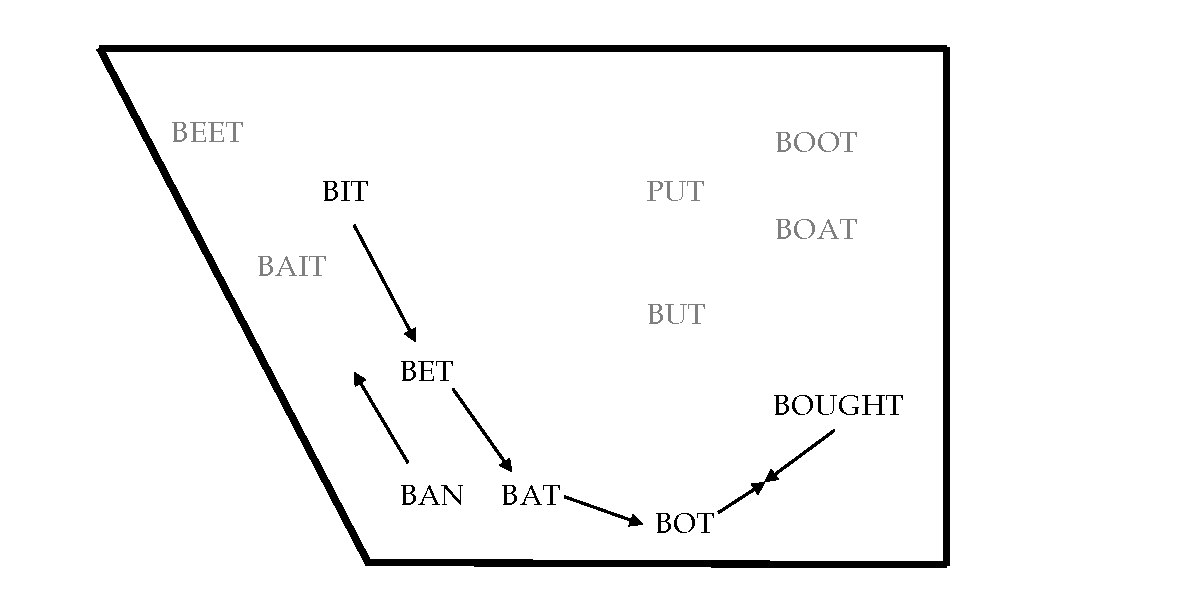
\includegraphics[width = 6.5in]{Figures/other_figures/cvs_diagram.pdf}
    \caption[The Elsewhere Shift]{The Elsewhere Shift. Vowels not included in this study are grayed out. Back vowel fronting, which some consider to a part of the Elsewhere Shift, is not indicated on this diagram.}
    \label{fig:elsewhere_shift_diagram}
\end{figure*}

Before proceeding, it is important to establish the labeling conventions that will be used for the remainder of this study. Of the labels that already exist to refer to vowels, such as IPA (/\textipa{\ae}/, /\textipa{E}/, /\textipa{I}/) and the set used by Labov and Trager \& Bloch (/\textipa{\ae}/, /\textipa{e}/, /\textipa{i}/), I have chosen to use the Wells lexical sets (Wells 1982: xviii–xix) when referring to broad phonetic categories,\footnote{See also \citet[43]{kennedy_grama_2012}, \citet{fruehwald_2018}, and \citet{stanley_2019_blog} for explanations of label conventions.} which are written in {\sc small caps} (i.e. \trap, \dress, \kit). However, when referring to allophones of these vowels, I use a mix of labels, some conventional and others less so. For example, recent volumes in the \textit{Publication of the American Dialect Society} series follow \citet{eckert_2008} and Thomas \& Yaeger-Dror's \citeyearpar{thomas_yaegerdror_2009} example of using the frame {\sc b\_t} (i.e. \bat, \bet, \bit) instead of the Wells labels. I also use these labels but only in reference to the elsewhere allophone of the phoneme itself. This makes it clear that, for example, \kit refers to the phoneme /\textipa{I}/ and \bit refers to any realization of \kit that is before obstruents. I likewise use the frame {\sc b\_n} for prenasal allophones (\ban, \ben, \bin). A more complete description of each of the allophones and their labels can be found in \S\ref{corpus_size_constitution}.




\section{Goals for this Study}
\label{goals}

To reiterate, this study contributes to this growing knowledge of the Elsewhere Shift by analyzing the vowels' formant trajectories and their variation and social meaning in Cowlitz County. Specifically, my goal is to convince the reader that there is evidence to support two hypotheses.

The first hypothesis is purely dialectological: The Elsewhere Shift is advancing in Cowlitz County. By ``Elsewhere Shift'', I mean the lowering and retraction of the preobstruent allophones of \trap, \dress, and \kit; the raising of the prenasal allophones of \trap, \dress, and \kit; and the presence of the low back merger. Evidence to support this hypothesis would take the form of vowel plots and statistical analysis showing that younger speakers have shifted vowels in the direction of the Elsewhere Shift. The null hypothesis is that the Elsewhere Shift is not advancing in Cowlitz County, meaning that older people and younger people's vowel spaces are similar and their front lax vowels are not shifted.

The second hypothesis for this study is sociophonetic in nature: Vowel trajectories provide crucial insight into how the Elsewhere Shift progresses in a community. Evidence to support this hypothesis would be to show that vowel trajectories provide additional insight into how vowels in the Elsewhere Shift change. The trajectories should change in a meaningful way as the relative position of the vowel changes. Importantly, this change in trajectory shape should uncover new information about the shift that a single-point analysis would miss, such as a distinction in the low back vowels (see Chapter~\ref{ch:low_back}). The null hypothesis is that vowel trajectories are strictly phonetic and provide no sociolinguistic information. For example, it may be the case that younger speakers have shifted vowels compared to the older speakers, but both group's vowel trajectories are similar.\footnote{In legacy data from the American South, we found this very phenomenon: vowel positions changed but their trajectories do not \citep{stanley_renwick_2020_LSA_talk}.} In this scenario, trajectories provide little additional information that the midpoints alone do not already provide.

As a way to study vowels beyond their midpoints, this study utilizes a method that has not been fully explored in American English dialects. Specifically, I use generalized additive mixed-effects models \citep{wood_2017} to analyze the formant dynamics of these vowels. While some researchers have analyzed vowel trajectory in relation to the Elsewhere Shift in the West, this study is the first to do so use this particular statistical model. Not only does this technique provide additional clarity in the realization of these vowels, but it uncovers variation in a vowel's \textit{trajectory}---not just relative \textit{position}---that has not been reported in other western communities.

\section{Organization of chapters}

In Chapter~\ref{ch:lit_review}, I provide a more thorough review of the literature in relation to speech in the West and the Elsewhere Shift. This shift is not yet fully understood, and different communities undergo the shift in different ways. I pay particular attention to the regional distribution of the Elsewhere Shift, pointing out that it has not yet been described in Washington. I also illustrate the conflicting accounts of how the shift is progressing in these different regions. I describe the structural relationship between the vowels, and theoretical accounts for the shift (i.e., whether it is a pull chain, a push chain, or a parallel shift). I also devote attention to the social meaning of the Elsewhere Shift, and what speakers index and listeners perceive when innovative variants are used.

Before moving to the study, I pause and use Chapter~\ref{ch:cowlitz_county} to outline the history of Cowlitz County. There were three reasons for the inclusion of this chapter. First, because this is the first linguistic analysis in this community, I felt it was appropriate to provide additional context so that the reader may better understand the geography, history, and culture of the community. Second, Washington was settled relatively late compared to the rest of the country and Cowlitz County especially was even later than other parts of the Pacific Northwest. In fact, we have a record of the names and origins of the first white settlers in the area now known as Cowlitz County; the Founder Effect \citep{mufwene_1996} may be an important factor when explaining language in this area. Finally, I include this chapter because in the results chapters I find that major historical events (the founding of Long-Bell in the early 1920s, and the change in the timber industry in the late 1970s) correlate with linguistic changes in the area.

Chapter~\ref{ch:methodology} describes the methods used in this study. Sociophonetic research involves many steps to get from fieldwork to statistical analysis. I explain the traditional fieldwork methodology utilized in this study, transcription, forced alignment, formant extraction, filtering, and normalization procedures. For some of these data processing tasks, I describe a few methods that are reported in the literature, evaluate the pros and cons of each method, and justify why I selected the procedure used here. I then describe the corpus size and constitution, providing a full description of the vowel classes in this study. Because sociolinguistic research is becoming increasingly quantitative in nature, I then provide a brief history of the methods used in variationist studies and justify the need for analyzing vowel dynamics. I provide details on how generalized additive mixed-effects models were implemented and then explain the visualizations that will be used in this study and how to interpret them. Finally, I describe how vowel shifting has been quantified in other studies and why I believe the typical method (comparing formant values to the ``benchmarks'' in the \textit{Atlas of North American English}) is inappropriate. It is my hope that this chapter provides a useful summary of the methods used in variationist studies and that others may become more informed regarding the statistical and analytical tools they use.

Chapters~\ref{ch:elsewhere_shift}--\ref{ch:low_back} present the results of this study. Chapter~\ref{ch:elsewhere_shift} deals with the front lax vowels before obstruents and demonstrates that the Elsewhere Shift is very much present in Cowlitz County speakers. Chapter~\ref{ch:prenasal} focuses on these three vowels before nasals, establishing that the prenasal split applies only to \trap and not \dress or \kit. I also focus on these vowels before /\textipa{N}/ because they appear to exhibit a different type of variation than the other prenasal environments, and because a full account of these vowels, particularly their formant trajectories, has not been completed in the West. Finally, Chapter~\ref{ch:low_back} presents results from the low back vowels, illustrating that the two vowels are not fully merged, but that they have been in a state of near-merger for several generations. At the end of each of these chapters, I discuss what the implications are for these findings, such as how the vowels are structurally related, what the results say about the diffusion of the shift, and a justification for the use of generalized additive mixed-effects models.

In Chapter~\ref{ch:discussion}, I summarize the findings and focus on a different source of data---the \textit{content} of the interviews---to describe the social meaning of the Elsewhere Shift. While a full-fledged 3rd Wave \citep{eckert_2012} analysis was not employed in this study, these speaker comments do illustrate a small portion of what these shifted vowels mean. Furthermore, I show that while older people enjoy their community, younger people do not and instead orient themselves towards Portland.\footnote{It is noteworthy that the younder speakers' orientation is towards the nearest urban center rather than an urban center within their own state. It is common in dialectology research to focus on a single US state. A fruitful area of research would focus on state boundaries and how dialect features and speaker orientation crosses those boundaries, such as the Kansas-Missouri state line \citet{strelluf_2019} and the United States--Canada line \citet{swan_2016_diss}.} This drastic generational shift can be explained by considering the history of the community, particularly the economic recession in the 1970s and 1980s, and I suggest here that these major historical events were perhaps the reason for the adoption of innovative speech variants by the youngest generations.


Finally, in Chapter~\ref{ch:conclusion}, I provide an overview of the work, discuss the limitations and point out directions for future work. In particular, I list many of the infrequent linguistic variables that were heard among these speakers, suggesting a high degree of variation in this community.

In addition to these chapters, I have also included several appendices. Some include supplementary methodological information like the reading passages, wordlist, and minimal pairs used in the interview and the list of stopwords that were excluded from analysis. Other appendices are related to the statistical output because they are too large to be comfortably included in the results chapters: summaries of the statistical models, model comparisons, and large multi-panel plots that show difference smooths and spectrogram-like visualizations. References to specific tables and visualizations are included throughout the text and this PDF includes internal hyperlinks to help guide the reader to this supplementary material.

It is my hope that this work succeeds in filling in one small hole in our dialect map of the United States and that the thorough description of vowel dynamics here will serve as a useful point of comparison in future studies on vowel trajectories.
   % 4,544 words
\clearpage\chapter{Western American English}
\label{ch:lit_review}




\section{Introduction}
\label{sec:lit_review_intro}

In the spring of 1986, Leanne Hinton led a graduate seminar at the University of California, Berkeley to study the pronunciation of English in California at that time. They noted that earlier studies on California English described the variety as relatively unremarkable, lacking distinctive features of its own. For example, Allan Metcalf, in a report on the \textit{Linguistic Atlas of the Pacific Coast} (\textit{LAPC}), says,
\begin{quote}
    The pronunciation of English in California and Nevada is unobtrusive, a bland blend of patterns found in the north and midlands in the eastern United States. To the linguist as well as to the untrained ear, it most often seems to be an American English `shorn of all local peculiarities' [\citep[192]{pei_1967}]---like the dog in the Sherlock Holmes adventure of Silver Blaze, notable for not being noticed \citep[8]{metcalf_nd}.
\end{quote}
However, in parodied imitations of Californians in the media, Hinton and her students noticed exaggerated phonetic features that were not found in early phonetic descriptions from the area. Had the language of California changed? The goal of the seminar was to compare their findings to the 270 Californians interviewed in the 1950s as part of the \textit{Linguistic Atlas of the Pacific Coast}.

Their results, eventually published as Hinton, Moonwomon, Bremner, Luthin, Van Clay, Lerner, \& Corcoran \citeyearpar{hinton_etal_1987}, became a pivotal study in speech in the West because they were perhaps the first to document the lowering and backing of \kit, \dress, and \trap in California. They found that younger, white, urban speakers tended to exhibit these patterns the most and proposed that these changes were the beginnings of a new shift in California English: ``[i]t is quite possible, then, that these new sound shifts will progress along the lines of many other California phenomena, becoming more extreme and spreading geographically'' \citep[126]{hinton_etal_1987}. While other studies have shown that these patterns have indeed spread across the West (cf. \citealt{fridland_etal_2016_pads}; \citealt{fridland_etal_2017_pads} inter alia), in this chapter I will show that they have spread geographically into Cowlitz County, Washington, providing the first conclusive evidence that the shift can be found in the speech of Washingtonians.

\subsection{A note on terminology}
\label{sec:terminology}

The vowel shift described by \citet{hinton_etal_1987}---the lowering and retraction of the front lax vowels \bit, \dress, and \bat---now goes by many names. In this study, I refer to it as the \textit{Elsewhere Shift}\footnote{\citet[20]{strelluf_2019} points out that the term was used ``somewhat jokingly'' at NWAV in 2016. I was not present at that conference, so I missed that connotation. Nevertheless, I will continue to use this term.}. As justification for using this term, this section explains the other names that have been used and why \textit{the Elsewhere Shift} was selected as the most appropriate for this study.

The most common terms for this vowel pattern describe where in North America it can be heard. One of the most popular names is the \textit{(Northern) California Vowel Shift}, coined by \citet{eckert_2008} because the shift has primarily been documented in the speech of Californians (cf. \citealt{hall_lew_etal_2015, janoff_2018, podesva_2011, podesva_etal_2015, villarreal_2016_pads, villarreal_2018} and many others). However, in light of recent research showing the presence of these changes in Nevada \citep{fridland_kendall_2017_pads}, Oregon \citep{conn_2000_diss, nelson_2011, becker_etal_2016_pads, mclarty_etal_2016}, Colorado \citep{holland_brandenburg_2017_pads, holland_2019}, Arizona \citep{hall_lew_etal_2017}, and New Mexico \citep{brumbaugh_koops_2017_pads}, the editors of the \textit{Speech in the Western States} volumes \citep{fridland_etal_2016_pads, fridland_etal_2017_pads} propose that the label \textit{Western Vowel Pattern}\footnote{Actually, as early as 2004, the term \textit{Western Vowel Shift} was used to describe this pattern in Arizona \citep{hall_lew_2004}.} be used. Meanwhile, because of its presence across most of Canada, the term \textit{Canadian Shift} has been used as well  (\citealt{clarke_etal_1995, boberg_2005, sadlier_brown_tamminga_2008, roeder_jarmasz_2010, kettig_2014} and many others) because they are ``talking about Canadians'' \citep{li_etal_2018}. These differences in terminology also reflect the trend that research in California and Canada has progressed more or less independently. Furthermore, when Californians and Canadians are compared directly, there are slight differences \citep{kennedy_grama_2012, hagiwara_2006} leading some to argue for the need to differentiate the two patterns.\footnote{For example, \citet[49]{kennedy_grama_2012} use the benchmarks provided in the \textit{Atlas of North American English} to define whether a speaker’s vowels are shifted. Most of their sample lowers \kit, \dress, and \trap past the threshold that defines the Canadian Shift, but their tokens of \lot cluster around the threshold. They conclude that because the front vowels were lowering while \lot was not sufficiently backed, ``it suggests that the California Shift is a different phenomenon from the Canadian Shift.'' However, based on the Short Front Vowel Shift Index (see \S\ref{how_shifting_is_measured}), which does not consider the low vowel(s), \citet[21]{boberg_2019} states that the shifts in California and Canada are, ``for all intents and purposes, the same thing.''}

A few of the other proposed labels for this vowel pattern are more descriptive of the vowels themselves, rather than the geographic regions involved. For example, \citet{hickey_2018} uses the term \textit{Short Front Vowel Lowering}. And Boberg \citeyearpar{boberg_2019} uses a similar term, the \textit{North American Short Front Vowel Shift}, as opposed to the \textit{New Zealand Short Front Vowel Shift}, in which the vowels move in the opposite direction from what is described here. Most recently, the term \textit{Low-Back-Merger Shift} has been proposed \citep{becker_2019_pads}, which makes the controversial theoretical stance that the shift is triggered by the low back merger.

Finally, there are labels in circulation that make no direct reference to geographic regions or vowels. \citet{labov_1991} may have been the first to assign a name to parts of to this pattern, the Third Dialect.\footnote{\textit{Third Dialect} more formally refers varieties that have the low back merger and /\textipa{\ae}/ being realized as a low front vowel, except before nasals where it is raised \citep[30]{labov_1991}. Given that bulk of that paper was written in 1980 (p. 34) and that the shifting in the front lax vowels in Third Dialect regions has only been documented since then, it is unclear whether the label should be applied to the lowering and retraction of front vowels, even if they are a consequence of the low back merger.} This is useful for researchers who study both the Pacific Coast and Canada \citep{swan_2018} or neither region \citep{durian_2012_diss}. The term \textit{Elsewhere Shift} has also been proposed to serve this purpose, with \textit{elsewhere} presumably refering to varieties that do not participate in the Southern Vowel Shift or the Northern Cities Shift, though this is relaxed somewhat due to the possible influence of both the Northern Cities Shift and the Elsewhere Shift in the same region \citep{mason_2018}. The term \textit{elsewhere} may also refer to the elsewhere allophones of the front lax vowels, which are the ones that are involved in this shift. The term has not gained very much popularity, but the dual meaning of geographic and phonological distribution is appealing.

For this dissertation I have opted to use this term, the \textit{Elsewhere Shift}. Terms that refer to geographic regions (\textit{California Vowel Shift}, \textit{Canadian Shift}, \textit{Western Vowel Pattern}) inadvertently exclude areas outside of some region where the pattern can be found. The terms \textit{Short Front Vowel Lowering/Shift} are descriptive enough when only \kit, \dress and \trap are included for study, but since the low back merger may be related to this lowering, at least in Western American varieties (see \S\ref{sec:structure_of_elsewhere_shift}), I argue that the label does not fully capture the shift. Thus, the geographic and vowel-ambiguous terms \textit{Elsewhere Shift} and \textit{Third Dialect} appear to be most appropriate presently for this study.

Another reason to use the term \textit{Elsewhere Shift} is because it appears to apply to the elsewhere allophones of the front lax vowel phonemes. For example, the \trap vowel can be divided into many different allophones, including prelateral, prerhotic, prenasal, pre-/\textipa{N}/, and pre-/\textipa{g}/\footnote{These allophones and their labels are explained in detail in \S\ref{word_classes}.}. But the elsewhere allophone, that is \trap before obstruents (except /\textipa{g}/), is the one that appears to be mostly consistently affected by the Elsewhere Shift. Similar patterns can be found with \dress and \kit. Therefore, the term \textit{Elsewhere Shift} appears to apply appropriately to geographic regions not part of the Northern or Southern Shift as well as the allophones not otherwise involved in some other phenomenon.

Finally, what vowels are included in the Elsewhere Shift? Some authors consider all Western features to be a part of the shift, including the lowering and retraction of front lax vowels, the low back merger, and the fronting of back vowels \citep{eckert_2004, eckert_2011, podesva_2011, podesva_etal_2015, donofrio_etal_2017_pads, donofrio_etal_2019}. Meanwhile, Boberg takes the stance that back vowel fronting occurs ``coincidentally, rather than causally'' with the shifting front lax vowels \citet[12]{boberg_2019}. For the purposes of this dissertation, I will use the term the \textit{Elsewhere Shift} to refer only to the front lax vowels as distinct shifts from the low back merger. The fronting of back vowels will not be considered in this study and thus is not a part of the definition of the term as I use it here.




\section{Geographic distribution of the Elsewhere Shift}
\label{sec:geography_of_elsewhere_shift}

Since that graduate seminar in Berkeley, numerous studies have documented the Elsewhere Shift in many parts of English-speaking North America. The low back merger specifically has been documented extensively in California \citep{moonwomon_1991_diss, hagiwara_2005, holland_2014_diss} and to a lesser degree in New Mexico \citep{brumbaugh_koops_2017_pads} and Montana \citep[122]{bar_el_etal_2017}. In Oregon, \citet{mclarty_etal_2016} find that both younger speakers and older archival speakers have a high degree of overlap between the two vowels, suggesting that the merger has been present for several generations. Similarly, the merger is found in Washington, even among the oldest speakers today \citep{wassink_2015, wassink_2016_pads}. In some studies, the two vowels are assumed to be merged without further commentary \citep{eckert_2008, podesva_2011, kennedy_grama_2012}.

As for the front lax vowels, the \textit{Atlas of North American English} actually did not find shifting in the West, stating that ``the West’s means for the short vowels\ldots do not stand out from the others, but are found slightly below the center of the main distribution. The West does not participate strongly in the Canadian Shift'' \citep[284--285]{labov_2006}. However, more focused studies with recent data have found evidence to support \citet{hinton_etal_1987}. For example, just focusing on \trap retraction, \citet[16]{donofrio_etal_2017_pads} find that younger people use increasingly retracted variants, especially the women, in California's Central Valley. \citet{kennedy_grama_2012} show that all speakers under the age of 30 in their sample lowered \trap, \dress and \kit, and \citet{holland_2014_diss} provides evidence that women and younger speakers have lower or backer variants of all three vowels, suggesting a change in apparent time. Similar patterns were found with respect to each of these vowels in San Francisco \citep{hall_lew_etal_2015, cardoso_etal_2016_pads}, Santa Barbara \citep{janoff_2018}, and elsewhere in California \citep{brotherton_etal_2019}. Thus, it is apparent that these vowels are indeed lowering in California.

In addition to studies focusing on California English, researchers further north into Oregon have likewise documented the Elsewhere Shift, though the patterns are less clearly defined. With speakers based primarily in the Southern Willamette Valley, the area closest to California, \citet{nelson_2011} finds that younger speakers are lowering \kit, backing \dress, and lowering and backing \trap. Further north into Portland, \trap is certainly retracting and lowering, but it is unclear whether \dress and \kit are too \citep{conn_2000_diss, becker_etal_2013}. Recently, \citet[116--118]{becker_etal_2016_pads}  have found that 74\% of their sample retracted \trap, with age as a significant predictor but not gender. However, they find that only a third of their speakers lower \dress, with women participating more in this shift. Even fewer people (just three in their sample of 34) had \kit lowering. \citeauthor{becker_etal_2016_pads} therefore propose an implicational hierarchy: \kit lowering implies \dress lowering which implies \trap retraction. However, in a study of the shift over real and apparent time in Oregon, \citet{mclarty_etal_2016} find that both younger and older speakers shift all three vowels, though the older speakers do so to a lesser degree. However speakers from archival recordings have very little evidence of the shift. While there may be differences in the minutia of the shift, these Oregon-based studies all point to the idea that the Elsewhere Shift is less uniform than it is in California and that it has developed slowly over several generations with younger speakers shifting more vowels and to a greater degree than older speakers. Furthermore, it appears that the lowering of lax vowels in Oregon is a pull shift since \trap is the most advanced, followed by \dress, and then \kit.

While researchers were documenting this vowel shift along the Pacific Coast, the same patterns were independently being found in all parts of Canada. \citeauthor{clarke_etal_1995} find it in speakers primarily based in Toronto and say that it is ``superficially\ldots virtually identical'' with the shifts in California \citeyearpar[213]{clarke_etal_1995}. In Toronto, the shift is equally robust across ethnicities \citep{hoffman_2010} and in other parts of Ontario it is almost as advanced as it is in the capital \citep{roeder_2012} though it is nearing completion \citep{roeder_jarmasz_2010}. Towards the east, early reports in Ottawa find that retraction of \trap is being led by younger women (\citealt[151--153]{woods_1979}; \citeyear{woods_1993}, \citealt{de_wolf_1992}), which is confirmed, together with \dress and \kit retraction, in more recent data \citep{boberg_2005}. Even though \textit{Atlas of North American English} reports that the Canadian Shift has not spread as far eastward as the Atlantic Coast \citep[220]{labov_ash_boberg_2006_anae}, the shift is found to be active in St. John's, Newfoundland (\citealt{hollett_2006},  \citealt{darcy_2005}, see also \citealt{clarke_1991}) and Hallifax, Nova Scotia (\citealt{sadlier_brown_tamminga_2008}; see also \citealt{boberg_2008}). Though it is less advanced than in other parts of Canada, the shift is also present in the Canadian Prairies \citep{boberg_2011, hagiwara_2006}. Finally, it is found to be most advanced in Vancouver \citep{hall_2000, tamminga_sadlier_brown_2008, roeder_etal_2018}, approximately equally across ethnicities \citep{presnyakova_etal_2018}, with women about a generation ahead of men \citep{esling_warkentyne_1993}. It is clear then that the Elsewhere Shift is as widespread and vigorous in Canada as it is in California and Oregon, especially in British Columbia. However, the two have been treated as ``independently occurring phenomen[a]'' \citep[41]{kennedy_grama_2012} in the majority of studies, with \citet{boberg_2019} and the work by Julia Swan (see below) as some of the few exceptions linking the two.

Conspicuously absent from these many regions where the Elsewhere Shift can be found is Washington. Despite pressure from California and Oregon to the south and from British Columbia to the north, Washington has appeared to resist the ever-reaching influence of the Elsewhere Shift: ``[i]t is curious that Canadian and California English should display such a similar trend while not being geographically contiguous neighbors of each other, since there is currently no evidence documenting the same type of shift in the geographic space between them'' \citep[30--31]{swan_2016_diss}. Alicia Wassink has stated that the Elsewhere Shift is not present in Washington: ``Seattle Caucasians do not participate in the retraction of /\textipa{\ae}/ \bat and /\textipa{E}/ \bet\ldots Additionally, we do not see the lowering of the /\textipa{I}/ \bit and /\textipa{E}/ \bet vowels'' \citeyearpar[84]{wassink_2016_pads}. She posits that Washingtonians' lack of participation in the Elsewhere Shift ``may be functioning as an important marker, distinguishing subregions in the West'' \citep[53]{wassink_2015}.\footnote{This lack of the Elsewhere Shift in Washington strengthens the argument I make in chapter \ref{ch:discussion}, which is that younger speakers orient themselves more towards Portland rather than to other Washingtonians.}, I suggest that the presence of the shift in Cowlitz County Washington is a large state with relatively few linguistic studies focused on its residents, so more work is needed to accurately describe the presence or absence of the shift in all parts of the state. But if the Elsewhere Shift is to be found in Washington, it would bridge the gap between California and Canada, perhaps finally uniting the two linguistic phenomena as a Pan--North American sound change. Or, if differences between the California and Canadian vowel shifts persist, then its manifestation in Washington would provide for an intriguing case of competing---albeit very similar---linguistic features.

However, one reason for why relatively little is known about the Elsewhere Shift in Washington may have to do with the history of dialectology in the state. As described in Chapter \ref{ch:introduction}, there was relatively little research on English in Washington before ten years ago, possibly because the speech in that area was considered to be devoid of regional characteristics, even more so than California. However, when Alicia Wassink and her colleagues introduced prevelar raising as a feature of Pacific Northwest English in 2009\footnote{Prevelar raising is the raising of \trap before /\textipa{g}/, so that words like \textit{bag}, \textit{flag}, or \textit{dragon} are pronounced with [\textipa{E}] or even [\textipa{e:}]. It was already known to be a part of Wisconsin English, but as far as I can tell, \citet{wassink_etal_2009} were the first to describe this feature in the Pacific Northwest. It has later been described in many regions of North America \citep{stanley_2019_BEG_paper}, but it is one thing that makes Washington stand out among the western states \citep{wassink_2016_pads}.}---especially since there were only isolated occurrences of it in the \textit{Linguistic Atlas of the Pacific Northwest} (i.e. Reed \citeyear{reed_1956}, \citeyear{reed_1961})---that set the tone for subsequent research questions for the next decade in Washington. Ever since that presentation, the majority of acoustic research on Washington English has focused on prevelar vowels and their distribution across regions, ages, genders, ethnicities, and other ideologically-based social groups (\citealt{wassink_2011, wassink_2015, wassink_2016_pads, freeman_2014, riebold_2015_diss, swan_2016_proceedings, stanley_2018_pwpl} and many others). To my knowledge, very few studies have looked at the front lax vowels in Washington outside of the prevelar environment.

One exception is Julia Swan’s research, which has focused on the direct comparison of English in Seattle, Washington and Vancouver, British Columbia. Though she, too, primarily describes differences in the realization of prevelar vowels, \citet[8]{swan_2016_proceedings} finds that retraction of \trap before fricatives (as opposed to stops) is more advanced for Vancouver speakers than it is for Seattle speakers, a pattern described in Canada by \citet[214]{clarke_etal_1995} and \citet{boberg_2019}. Furthermore both groups have nearly identical trajectories for pre-/\textipa{d}/ tokens of \trap \citeyearpar[10]{swan_2016_proceedings}, and F2 measurements were not statistically significantly different from each other in pre-obstruent environments \citep{swan_2015}. Given that Vancouver is the part of Canada where the Elsewhere Shift is most advanced \citep{hall_2000, tamminga_sadlier_brown_2008, roeder_etal_2018}, Swan indirectly reports that \trap retraction may be found in Seattle.

In summary, the Elsewhere Shift can be found in a very large geographic area of North America. It extends across all of Canada, and along the Pacific Coast from Southern California to at least as far north as Portland. It can even be found in areas not traditionally part of Third Dialect regions such as Hawaii \citep{grama_etal_2012, kirtley_etal_2016}, Alaska \citep{bowie_etal_2012}, Ohio (\citealt{durian_2012_diss}; \citealt[20]{thomas_2001}), Illinois \citep{bigham_2010}, Michigan \citep{nesbitt_mason_2016, mason_2018}, Texas \citep[20--21]{thomas_2001}, Massachusetts \citep{stanford_etal_2019}, and Georgia \citep{stanley_2019_LCUGA6}. If it is the case that speakers in Washington are clinging to traditional variants, we have a noteworthy case of resistance to such a widespread change, which may be grounded in strong opposition to the ideological personae expressed in these variants. However, as this study reports, many speakers in Cowlitz County \textit{do} have the Elsewhere Shift in their speech, meaning that they are participating in the macro-level changes of the region. In other words, they are distinguishing themselves from Seattleites. These findings provide some evidence against the claim that Washington is resisting the change and suggests that the shift has crossed the border into Washington.




\section{A structural description of the Elsewhere Shift}
\label{sec:structure_of_elsewhere_shift}

As a consequence of this large amount of research on front lax and low back vowels in North American English, we have learned a great deal about the structure of this shift. However, the degree to which vowels shift varies across regions and from study to study, and many questions remain regarding the structural relationship between the front lax vowels and their connection to other shifting vowels.

\subsection{The position of the low back vowel(s)}
\label{position_low_back_vowels}

The most defining feature of Western American English is the low back merger \citep[277]{labov_ash_boberg_2006_anae} and has been reported in numerous communities. As far as how the two vowels are merging, there are different reports of this process. In the West, it has been found that \thought lowers and fronts to merge with \lot \citep{hall_lew_2013}. In Utah, just the opposite was found: \thought was remarkably stable in real time, and it may have been \lot that backed to merge with \thought to result in a backed merged vowel \citep{bowie_2017_pads}. \citet{donofrio_etal_2017_pads} report a similar pattern in California's Central Valley. Most famously, \citet{herold_1990_diss} proposes a merger by expansion in which the distinction between the two is simply lost, and speakers realize tokens anywhere in the combined vowel space of the two historical vowels.

Regarding the relative position of the merged vowel, there is variation across studies. \citet{holland_brandenburg_2017_pads} find that the F2 of the merged low back vowel is decreasing in apparent time, suggesting that the vowel is getting more backed. Furthermore, \citet[23]{donofrio_etal_2017_pads} report that in Redding, California, the two vowels merged first, and then the now-merged vowel raises to a position that is higher than most other regions in the United States, creating a triangular vowel space with \bat as the lowest vowel; in Bakersfield and Merced, this higher merged vowel was achieved by \lot raising to meet the stably high \thought. This raising of the merged vowel, accompanied with \bat-retraction and \bet- and \bit-lowering creates an elegant description of a rotated vowel space as a result of the Elsewhere Shift. There are some exceptions (such as the relatively fronted merged vowel in Washington reported by \citealt{wassink_2016_pads}), but the general tendency is for the merged vowel to be backed and possibly raised.

However, what appears to be a more common finding in studies in the West is that speakers are on their way towards merging the two vowels. For example, \citet{moonwomon_1991_diss} analyzes the two vowels in a variety of environments and shows that the oldest speakers retain the distinction except before nasals and fricatives while the younger speakers all have a merger or a partial merger in all environments. \citet[367]{hall_lew_2013} reports that Chinese Americans had a more advanced merger, but it was not complete in San Francisco in 2008--2009. In Colorado, the two vowels were close, but \lot was consistently more fronted than \thought, especially for the men, suggesting a near, but so far incomplete, merger \citep{holland_brandenburg_2017_pads}. In Nevada, \thought is further back in the vowel space, but women are closing the gap \citep{fridland_kendall_2017_pads}. Most notably, \citep{dipaolo_1992} finds that \lot and \thought are distinct in Salt Lake City, despite other reports of merger in the region. Close to Cowlitz County, \citet{becker_etal_2016_pads} reports that nearly 40\% of their Portland-based sample retain the distinction.

These various studies point out that despite being a widespread feature of the West, there is a fair amount of variation. In some areas, the vowel is reported to be completely merged. However, there are pockets where the data suggests more of a near merger. In some areas, one vowel is stable in apparent time, with the other shifting towards it. The merged vowel is reported to be somewhat fronted, relatively backed, or backed and raised. However, in nearly every case, if the low back merger is not complete, it is on its way towards completion.

\subsection{The relationship between the front lax vowels}
\label{sec:relationship_between_front_lax_vowels}

In some ways, because \trap retraction occurs primarily in areas that have the low back merger, it is reasonable to propose that the merger of \lot and \thought was the start of a chain shift. This low back merger could have caused \trap to lower and retract to fill the void left by \lot, which in turn caused \dress and \kit to shift. In fact, \citet[139]{gordon_2006} proposes this very idea, that this merger is the underlying cause of the lowering and retraction of front lax vowels. He is supported by \citeauthor{clarke_etal_1995} who suggest that ``it is precisely the merger of the cot/caught vowel which serves as the pivot of the Canadian Shift'' (\citeyear[212]{clarke_etal_1995}; see also \citealt{dedecker_mackenzie_2000}; \citealt[220]{labov_ash_boberg_2006_anae}, \citealt{boberg_2019}). In an approach driven more by phonological theory, \citet{roeder_gardner_2013} propose that the merging of \lot, \thought, and \palm caused the restructuring of \trap, which in turn led to its retraction. A language-internal motivation for the shift accounts for the similarities between the Elsewhere Shift in California and Canada because migration patterns cannot do so. It also fits with a principle of chain shifts that Labov has proposed: ``lax nuclei fall along a nonperipheral track'' \citeyearpar[194]{labov_1994}. In theory, the chain shift hypothesis is an elegant explanation for the Elsewhere Shift.

However, phonetic data sometimes fails to support the hypothesis of a chain shift. First, it is unclear whether the low back merger is indeed the trigger. In Illinois, \citet{bigham_2010} finds the correlation between the low back merger and \trap retraction at a community level, but when examining individuals there were some speakers with the merger and no backing of \trap while others did not have the merger yet still had a backed \trap. In California, \citet[51]{kennedy_grama_2012} show that the merged low back vowel is not retracted as it is in Canadian speakers, but their speakers do have a lower and more centralized \trap. They take this to mean that the Elsewhere Shift may not necessarily have been triggered by the retraction of the low back vowel, at least in California \citep[see also][]{grama_kennedy_2018}. In fact, \citet[121]{holland_2014_diss} finds evidence against the low back merger being the trigger, and instead finds that---if the Elsewhere Shift is a chain shift at all---that the retraction of \dress may have been the trigger \citep[see also]{holland_2019}. Essentially, we find that each community appears to have different realizations of these vowels, and that a single explanation simply does not describe the phonetic patterns found in all areas with the Elsewhere Shift.

Furthermore, it is unclear whether the retraction of front lax vowels happened one at a time, as a chain shift would predict, or all in parallel. Some studies along the Pacific Coast find that the shifting of one vowel implies the shifting of another and propose an implicational hierarchy bearing the resemblance of a chain shift (\citealt[116--117]{becker_etal_2016_pads}; \citealt[121]{holland_2014_diss}). But others find parallel movement across generations with no indication that any one vowel moved first \citep{pratt_etal_2018, donofrio_etal_2019}. Furthermore, evidence from rural Ontario \citep{lawrance_2002_thesis} and Montreal \citep{boberg_2005} also suggest parallel movement of all three vowels. This discrepancy between how the Elsewhere Shift progresses over time further suggests that no one explanation can fully explain the phonetic data found in various communities.

% TODO: Renwick: Q. Is it really the case that vowels must be kept maximally distinct from one another? Is that Labov's position, or your position? Might there be particular models of vowel inventories that do or don't support this position? (Could you take a broader reach into the phonetic literature/motivations for this phenomenon, if it is real?)
Another possible explanation involves a combination of a chain shift and parallel changes. Chain shifts affect more than one vowel by means of a cause-and-effect relationship \citep[119--121]{labov_1994} and the underlying force driving these shifts is the need to keep vowels maximally distinct from one another.\footnote{Across the world's languages, vowels tend to position themselves around the edges of the F1-F2 space \citep[228,285]{ladefoged_johnson_2011}.}. While vowels may not be maximally distinct in the sense that they employ a host of secondary articulations and suprasegentals, at the very least, they need to be sufficiently perceptually distinct from one other to remain contrastive.). The movement of one vowel to fill the void left by another can account for the low back merger, \trap retraction, and the lowering of \dress and \kit, but it does not necessarily explain the retraction of \dress and \kit. Instead, the two higher vowels may simply move by analogy to the retraction of \trap (\citealt[232]{durian_2012_diss}; \citealt[151]{boberg_2005}), similar to back vowel fronting. This joint explanation has some merit because it appears to explain the patterns found in communities where the strict chain shift or strict parallel shift fails.

Finally, there are conflicting reports of whether the vowels retract (suggesting a lowered F2), lower (suggesting a higher F1), or both. Regarding the shift in Canada, \citet{boberg_2005} points out that while the difference may seem superficial, it has major implications for the structural nature of the shift. If \trap is retracting and \dress and \kit are lowering, that suggests a rotation in the vowel space that would be characteristic of a chain shift. However, if (as he finds in Montreal) the lax vowels primarily retract and retain the same height, this would be better described as a series of parallel shifts, akin to what is found with back vowel fronting in many varieties of American English and therefore not a chain shift. It is also possible that one pattern may be found in some varieties and another pattern is found in others.

In some cases, retraction and lowering are both reported, but they occur at different times within the same community. \citet[144]{boberg_2005} found lowering of \trap between the oldest and middle generations and then retraction of \trap and \dress between the middle and younger generations. Conversely, \citet{donofrio_etal_2019} find that \trap retraction occurred first in California and it was only the Millennials that have lowered it. In Lauren Hall-Lew's sample of residents of the Sunset District in San Francisco, younger participants and women produced a backer vowel, especially in the word list style (as opposed to the reading passage), where \bat was significantly lower as well \citep{hall_lew_etal_2015}. An analysis of these same speakers' conversation style found that similar results in regards to sex and age, only the primary dimension of change was height, not backness \citep{cardoso_etal_2016_pads}. All this goes to show that different processes can result in the same eventual outcome.







\section{The prenasal split}
\label{sec:prenasal_split}

The Elsewhere Shift applies to the elsewhere allophones of \trap, \dress, and \kit. However, in some cases, prenasal allophones of these vowels raise instead of lower, a phenomenon called the prenasal split. In other words, the distance between the prenasal and elsewhere allophones increases due to their movement in opposite directions. Thus, a full treatment of the Elsewhere Shift would be incomplete without a description of the variation found in this environment as well.

There are clear articulatory, acoustic, and perceptual reasons for why vowels in prenasal environment are raised. The articulation of a nasal consonant requires the opening of the velum to allow airflow through the nasal cavity. Because the velum is a relatively slow-moving articulator, anticipatory coarticulation occurs during the vowel in preparation for the following nasal. Therefore, for a portion of the duration of the vowel, air flows out both the mouth and nose, producing a nasalized vowel. Acoustically, a nasalized vowel differs from an oral vowel in various ways, including the presence of a strong concentration of energy in F1 region of frequencies called the nasal formant, which is the result of the nasal cavity being used as a resonating chamber. In a spectrogram, this nasal formant appears distinct from F1 of high and mid vowels, while it is indistinguishable from the F1 of low vowels other than widening its bandwidth \citep[193--194]{olive_etal_1993}. This extra nasal formant, particularly with \trap, causes vowels to be perceived as higher \citet{wright_1975}. This perception can be then be exploited by speakers to produce a higher vowel: \citet{dedecker_nycz_2012} show that some New Jersey speakers use tongue position to produce a tensed [\textipa{\ae}] while other use nasalization to simulate the auditory effect. \citet[334]{mielke_etal_2017} state that ``the most obvious explanation for the development of /\textipa{\ae}/ raising before nasals is that the acoustic effects of nasalization were transphonologized to tongue position.'' In other words, the side effects of the anticipatory coarticulation of the following nasal consonant are exaggerated onto the vowel itself, creating a raised variant that cannot be fully explained by phonetic effects alone. The \textit{Atlas of North American English} states that ``there is no doubt that nasal allophony has been translated to the phonological level,'' \citep[175]{labov_ash_boberg_2006_anae}  further supporting additional raising beyond coarticulatory effects.

\ban-raising specifically is well-attested in varieties with and without the Elsewhere Shift. Prenasal tokens were the most raised allophone of \trap in San Francisco \citep[43]{cardoso_etal_2016_pads} and Oregon \citep{becker_etal_2016_pads}. In fact, Thomas finds that prenasal raising ``occurs widely in North American English'' and that it ``appears to be largely a twentieth-century phenomenon'' \citeyearpar[52]{thomas_2001}. Its frequency in the West appears to be conditioned by ethnicity. Chinese Americans \citep[43]{cardoso_etal_2016_pads} and speakers of Chicano English \citep[34]{eckert_2008} have been shown to have less raising of \ban while Spanish speakers have a greater separation between \bat and \ban than California university students \citep{holland_2014_diss}.

Some researchers have described the specific realization of \ban in detail. It is transcribed with a central offglide, such as [\textipa{me\super @n}] \textit{man} \citep[34]{eckert_2008} or with a raised diacritic [\textipa{\|'\ae}] \citep[132]{gordon_2006}. When comparing trajectories of Seattle and Vancouver speakers, \citet{swan_2016_proceedings} describes the trajectory of \ban in Seattle as starting high and front and lowering and dramatically retracting over the course of its duration; in Vancouver it raises and backs gradually along its duration. These realizations are slightly different from the rising-falling pattern found by \citet{mielke_etal_2017}, which peaks just before the midpoint of the vowel. \citet{brotherton_etal_2019} find that secondary features like diphthongization and nasalization play important roles in differentiating \ban from \bat in the prenasal split. All these studies show that speakers with a greater prenasal split tend to have more diphthongization in \ban, suggesting that more trajectory-based research on this vowel is needed.

What is less clear is the extent to which \ben and \bin are raised. \citet[106--107]{holland_2014_diss} found evidence of \ben-raising in apparent time in California, but women’s \ben was lower and Spanish speakers’ was fronter. In a primarily Toronto-based sample, \citet{dedecker_mackenzie_2000} found that \ben and \bin were lowered less than in other environments, but this does not necessarily imply raising. In San Francisco, \bin was not any different from \kit and \ben actually retracted in apparent time at the same rate as other allophones of \dress, leading \citeauthor{cardoso_etal_2016_pads} to the conclusion that the nasal split does not apply to \dress \citep[43--44]{cardoso_etal_2016_pads}. Furthermore, there are some scattered reports of the \textit{pin-pen} merger in the West, such as in Riverside, California \citep[31]{metcalf_1972}, Trinity County, California \citep{geenberg_2014_diss}, Bakersfield, California \citep{warren_fulop_2014}, older Utahns \citep{lillie_1998_thesis}, and possibly Seattle \citep{scanlon_wassink_2010}. Thus, a hypothetical claim that all three front lax vowels raising before nasals is untenable based on research in West. It appears that the prenasal split applies chiefly to \trap, though further investigation on \ben and \bin is needed to understand what regional patterns there may be, if any.

Of particular interest is the velar nasal and its effect on the front lax vowels (\bang, \beng, \bing). Prevelar raising is known to affect vowels before /\textipa{g}/ (\bag, \beg, \vague) in the Pacific Northwest, the Upper Midwest, and Canada \citep{stanley_2019_ADS}, but voiced velars (that is, both /\textipa{g}/ and /\textipa{N}/) are not necessarily grouped together as a natural class because the two appear to be treated differently by different speakers.\footnote{The acoustic effect of a velar consonant on surrounding vowels is that F1 lowers, F2 raises, and F3 lowers, a phenomenon known as the \textit{velar pinch}. The degree to which this pinch affects a vowel is greater for /\textipa{N}/ than for /\textipa{g}/ because of the accompanying lowering of the velum \citep{baker_etal_2008}. Therefore, this tendency to raise, coupled with the auditory perception that low vowels are pereived as raised when nasalized (as discussed above), means pre-/\textipa{N}/ vowels have two forces acting upon them to encourage raising.} For example, \citet[46]{conn_2000_diss} finds that while Portlanders do have \ban-raising, for some speakers \bang is raised less than \ban and for others \bang is more fronted than \ban. Some studies separate all three front lax vowels, \kit, \dress, and \trap, into allophones that are followed by /\textipa{m}/ and /\textipa{n}/, and allophones followed by /\textipa{N}/. In other words, they analyze \bin, \ben, and \ban as distinct allophones from \bing, \beng, and \bang (which are all different from the elsewhere allophones \bit, \bet, and \bat). \citet[42]{cardoso_etal_2016_pads} were justified in this methodology because they found that \bing was raised more than \bin or \bit (see also \citealt{eckert_2004}), with women's realizations the highest, while \bin was not raised. They also find a significant effect for age on the height of \bang. For the purposes of this dissertation, I adopt this position and treat prevelar nasal environments distinct from pre(other)-nasal environments.

Summarizing the prenasal split, the role of nasal allophones and their relationship to the Elsewhere Shift is not as well-known as their oral counterparts. It is clear that the prenasal split applies to \trap and that the gap between the two allophones is widening in apparent time, but if the split applies to \dress and \kit, little evidence has been presented to support this. However, front lax vowels before /\textipa{N}/ do appear to be raising, at least in studies that have looked at them specifically, though the status of \beng is unclear due to the very low number of tokens containing that sequence. More work is needed to fully understand if and how prenasal tokens pattern together.

In Chapter \ref{ch:prenasal}, I shed light on the structural relationship of prenasal and pre-/\textipa{N}/ allophones of \trap, \dress, and \kit. The vowels' relationship to each other was tentative at best, suggesting that changes in prenasal environments in the West are perhaps driven by phonetics rather than by some larger phonological structure; changes are likely community-specific rather than being pan--North American.





\section{Social meaning in the Elsewhere Shift}
\label{sec:social_meaning_elsewhere_shift}

Finally, it is important to discuss the social meaning that is associated with the Elsewhere Shift. A large body of research has analyzed how listeners perceive shifted or unshifted variants, showing that people are sensitive to and assign social meaning to aspects of the Elsewhere Shift. Furthermore, speakers use these shifted variants and their associated meanings as a part of identity and persona construction.

Several studies have shown that the a retracted \bat vowel indicates a variety of social meanings to listeners. First, there is the negative association of the ``Valley Girl``, which is perceived as  shallow, materialistic, and unintelligent \citep[47]{donofrio_2016_diss}. Valley Girls, together with the male counterparts, ``Surfer Dudes'', were stereotyped in California-based songs, movies, and comedy in the 1980s and 1990s. Some of these stereotypes exist today, and a retracted \bat continues to index some of these attributes today.

However, an unrelated and contrastive social meaning associated with retracted \bat is that of professionalism and education. \citet[47]{donofrio_2016_diss} shows that speakers and listeners associate a backed or lowered \bat with formality, upper class, education, correctness. Overall they evaluated a more shifted \bat as evoking a business professional persona. In an in-depth analysis of a single woman's vowels, \citet{vanhofwegen_2017_diss} shows that speakers use stylized variants of vowels that are more peripheral, longer in duration, more likely to be creaky; specifically for \bat, the speaker used these stylized variants when ``taking a stance of knowledge during these interactions---she knows something her classmates do not'' \citeyearpar[149]{vanhofwegen_2017_diss}. \citet{podesva_etal_2012} analyzes the speech of Condoleeza Rice and show that she uses linguistic features that are associated with formality, being highly educated, and standardness, including released word-final voiceless obstruents and a backed \bat. \citet{donofrio_2018} points out that \bat may index these particular meanings because of how Americans typically view British English, and in particular, the \trap-\bath split. This lexically conditioned split is a part of some varieties of British English and the backer vowel is often perceived as more intelligent and correct. Indeed, \citet{boberg_1999} shows that American English listeners perceive /\textipa{a:}/ as more correct, educated, and sophisticated than /\textipa{\ae}/ in foreign words like \textit{llama}, \textit{pasta}, and \textit{drama}. These various factors combine to create an overall sense that the retracted \bat conveys a level of sophistication that the conservative front \bat does not.

% TODO: Dr. Renwick's comment on what is meant by wiggle room. I want to say it's because there aren't nearby vowels and that it's quite different acoustically from the others but I don't know if that's objectively true, and it sort of splits up the Pratt et al's description.
In addition to these primary meanings of ``Valley Girl'' and business professional persona, the indexical field for retracted variants of \bat include various additional meanings as well. \citet{geenberg_2014_diss} finds that speakers who had spent more time outside of their rural community in California used backer variants of \bat than those who did not leave the county. However, nearby in Redding, \bat was one of the few linguistic features that was \textit{not} associated with orientation towards the town verses the country \citep{podesva_etal_2015}. Among Chicano English speakers in Culver City, California, retracted \bat was used more by non-gang members than gang-members (and this distinction was more important than social class or language background), suggesting that these non-gang members are conforming more with the majority community as a part of their linguistic expression \citep{fought_2003}. \citet[150]{vanhofwegen_2017_diss} provides several examples of how a lowered \bat is used when a speaker expresses ``righteous indignation'' and calls for additional study on such extreme tokens to get a more complete picture of what these tokens mean. I believe \citeauthor{pratt_etal_2018}'s \citeyearpar{pratt_etal_2018} description of \bat describes it perfectly: there is a great deal of ``wiggle room,'' and speakers have been shown to exploit those different variants to serve a variety of multifaceted purposes.

% BAT outside of CA
For non-Californians, it appears that while a retracted variant of \bat carries less social meaning than it does in California, it is often associated with California itself. For example, in Oregon, \citet{adcock_becker_2016} find that listeners link a backed variant of \bat with California personae. And based on the perceptions of listeners from the Bay Area, Portland, and Seattle, \citet{becker_swan_2019} find the backed \bat was perceived as young and frivolous, which is possibly related to the Valley Girl stereotype that came out of California. Given the Californian stereotypes that are perpetuated with the Elsewhere Shift, these associations come as no surprise. In fact, based on the work of \citet{labov_1963}, \citet{eckert_2000}, and \citet{zhang_2005}, \citet[462]{eckert_2008_indexicalFields} shows that ``variables that historically come to distinguish geographic dialects can take on interactional meanings based in local ideology\ldots Local identity is never an association with a generic locale but with a particular construction of that locale as distinct from some other.'' In other words, we would not expect the full indexical field of retracted \bat to be the same across all areas of the West. Specifically, the ``business professional'' persona that is documented in California does not appear to transfer to other areas. However, its associations with California do.\footnote{That the shift occurs in California or indexes California may be reason enough to continue calling it the \textit{California Vowel Shift}. This association may be lost (or perhaps never existed) in areas far from the Pacific Coast though, so I will continue using the term \textit{the Elsewhere Shift}.}

Like any other variable, \bat has an indexical field that includes a variety of meanings, some of which are contradictory. Specifically, \citet{becker_swan_2019} also found that when listeners tried to guess where the speakers were from, retracted \bat was most correlated with being not from the West Coast, not from California, and possibly from Canada. In other words, the California-ness that some listeners assign to that variable is not universal. Instead, \citeauthor{becker_swan_2019} argue that, to these listeners, \bat retraction may just be a generic, supra-local, and unspecified feature. Additional work is needed on listener perception of the Elsewhere Shift to fully understand these social meanings.

% BAN-raising
In addition to \bat retraction, \ban-raising has been found to vary sociolinguistically in California. \citet{eckert_2008} focused on the nasal split in two schools separated by only a ten minute drive. In Fields Elementary, \ban is raised and in Steps Elementary, \ban is not. The majority of students at Fields are middle-class Anglos while students at Steps come from a poorer, ethnically diverse population where Chicano English has the most linguistic capital. But a lack of raising is more than just an ethnicity difference because it is used by children of all ethnicities, particularly to index the ``coolness that emerge[d] within the ethnic group'' \citeyearpar[41]{eckert_2008}. In a more rural part of California, Redding, \citet{podesva_etal_2015} found that a higher \ban vowel was used by younger, country-oriented males (as opposed to ``townies''). Given that the prenasal split is strongest among urban areas, it is somewhat surprising to find that this group lead the change. But \citeauthor{podesva_etal_2012} argue that because \ban-raising has become a pan-regional pattern of American English, these speakers' use of this new national norm is a result of their opposition towards the big California cities, even though a more extreme form of \ban raising is a part of California English.


% BET and BIT
While the amount of social meaning associated with \trap (that is, both \bat and \ban) is extensive, \dress and \kit appear to be less socially salient. For example, in their study of Condoleeza Rice's speech, \citet[76]{podesva_etal_2012} find that she did not shift these two vowels to indicate formality as she did with \trap. Similarly, some studies find that while other aspects of the Elsewhere Shift are advanced when constructing a particular identity, \bet and \bit do not change \citep{fought_2003, podesva_2011}. Nevertheless, in stereotyped parodic performances of Californians, \textit{Saturday Night Live} comedian Kristen Wiig uses significantly backed variants of all three vowels, though this is likely the result of her open-jawed setting that she uses extensively while portraying that character rather than social meaning of the vowels themselves, because in those same skits co-performer Fred Armisen does not shift his vowels in the same direction but does employ a distinctive jaw setting and lip protrusion \citep{pratt_donofrio_2017}.



% Moving to the low vowel
Moving to the low back merger, \citet{eckert_labov_2017} find that people do not generally associate social meaning to abstract phonological processes, like a vowel merger. They do, however, find that ``social meaning attaches to the individual shifts that bring about the merger'' \citeyearpar[484]{eckert_labov_2017}. This holds true with the Third Wave studies on the low back vowels. For example, \citep{pratt_2018} finds that tech students at a California high school used a higher \lot vowel than the other students did, indexing the ``toughness'' that is a part of being in that social group. On the other hand, \citet{hall_lew_2013} suggests that social meaning is associated with \thought, which is the reason for it being more fronted than \lot (resulting in a flip-flop in the vowel space). Exactly what that meaning is is difficult to pin down:
\begin{quote}
    ``[I]t may be that more advanced [{\thought}] tokens are a component of `Asian' styles, or just new local persona more generally. Perhaps an advanced [{\thought}] vowel was just one small part of the stylistic package that indexed `five-foot-tall Asian girl[s] who could breakdance'.'' \citet[381]{hall_lew_2013}
\end{quote}
In that study, what the three women that had the most fronted \thought shared was ``a lifetime of active negotiation between conflicting local authenticities'' \citeyearpar[386]{hall_lew_2013}. Similarly nuanced and complex meanings may be associated with the shifting low back vowels in other Western communities and additional work is needed to fully understand this variable.

% Overall vowel space
Finally, rather than dissecting the Elsewhere Shift into its constituent parts, several studies have shown that multiple linguistic variables shift in concert to index specific social meanings. For example, \citet{pratt_2018} shows that the ``toughness'' in the tech students mentioned above was also indexed with a more velarized /\textipa{l}/ and that the combination of the two is what conveys the social meaning. In an in-depth study of one gay California man's speech, \citet{podesva_2011} shows that a more advanced \bat-retraction, \ban-raising, and back vowel fronting are all used to in some situations to help the speaker construct a gay ``partier'' persona. He argues that it is the ``ways in which variables are combined and packaged'' (\citealt[41]{podesva_2011}, see also \citealt{campbellkibler_2011}) that index social meaning.


%Finally, among Californians, \citet[68]{villarreal_2016_pads} finds that that no part of the Elsewhere Shift was significantly correlated correctness, pleasantness, self-similarity, and place.

To summarize, many aspects of the Elsewhere Shift index a wide variety of social meanings. In California, retracted \bat is associated simultaneously with the ``Valley Girl'' and the ``business professional'' personae, while elsewhere it is often associated with California itself. \ban-raising, and both \lot and \thought have more varied meanings, and \bet and \bit have relatively little social meaning. Additional research will help us fully explore the ``wiggle room'' and socioindexical variation ascribed to these sounds.

\section{Conclusion}

% TODO: Renwick: Q. WE NEED A SCHEMATIC PLOT HERE... (Please draw it on the board) --> actually this should just be the Elsewhere Shift schematic from your presentation slide 2
For the purposes of this study, the Elsewhere Shift will be defined as the lowering and/or retraction of the front lax vowels, the raising of \ban, and the merger or near-merger of the low back vowels (possibly accompanied with raising). Numerous studies have documented the presence of all or parts of the Elsewhere Shift in many regions of North America. However, the precise nature of the shift (both the trajectory of change and its relative timing) exhibits a large amount of variation, which has led to different conclusions about the structural relationship between the shifting vowels.

%TODO Q. It is not clear to me WHICH VOWELS YOU WANT TO STUDY. There seems to be no set of "research questions" laid out, and there is no chapter or section heading called "research questions" or "goals" or anything similar -- instead, it's as if you are just reacting to others' work, when in fact you have done an enormous amount of thinking and analysis. Make it clear what your contribution sets out to be, and give us signposts to it.
%TODO I wonder if a solution could come from my other comment about whether people identify more with Seattle or with Portland. For instance, you can explicitly test (a) whether Cowlitz Countians participate in the Elsewhere Shift, and (b) whether that has participation has increased over generational time. If (a) is true, this is evidence that people lean more towards Portland than Seattle, which perhaps is surprising given that CC is in Washington State (but Portland is closer geographically); if (b) is true, this is evidence in favor of your argument that social/economic change in CC has led to, or is related to, linguistic change over time.
     % 6,951 words
\clearpage\chapter{Cowlitz County, Washington}
\label{ch:cowlitz_county}

As this is the first linguistic analysis of the speech in Cowlitz County, I felt that a brief description of the area was requisite because it is necessary to understand the context in which these linguistic changes are embedded. I will briefly describe the area's geography since the abundance of trees and proximity to rivers ultimately played an important role in the growth of the timber industry there. What then follows is a brief history of the region, including the Cowlitz people, the settlement of the first people of European descent, colonization, Longview and the Long-Bell Company and the demographic shift that ensued, and the rise and fall of the mills during the 20th Century.

This chapter draws heavily from four sources. The first is a small book entitled \textit{Cowlitz County Washington 1854 - 1948} written by Hattie Barlow Olson\footnote{Her name as it appears on the book is Mrs. Charles H. Olsen but \citet[177]{urrutia_1998} mentions her by name.} and published by the Kelso Chamber of Commerce in 1948. Olson's parents were some of the original founders of Kelso and she relates several first-hand accounts of the early days of Cowlitz County. The second work is \textit{They Came to Six Rivers: The Story of Cowlitz County} by Virginia Urrutia, published by the Cowlitz County Historical Society in 1998. Urrutia is also a descendent of some of the original founders of the area and a long-time editor of the \textit{Cowlitz Quarterly}. Another is \textit{R. A. Long's Planned City: The Story of Longview} by John M. McClelland, Jr., published by the Longview Publishing Co. in 1976. McClelland is the son of the first editor of the local paper, the \textit{Longview Daily News}. The last is \textit{Whistles: The Story of Longview Fibre Company} by David Wilma, a historian with family ties to the area, who personally interviewed many longtime residents.\footnote{I am grateful to David Wilma and also to Bill Watson of the Cowlitz Historical Museum for sharing with me the audio to many of these interviews and many other recordings of lifelong Cowlitz County residents. I acquired them too late for them to be incorporated into this dissertation, but they will provide an invaluable source for tracking language change in real time in southwest Washington. } A few details from my own interviews are sprinkled throughout where relevant.

\section{A physical description of Cowlitz County}
\label{sec:physical_description}

\begin{figure*}[p]
    \centering
    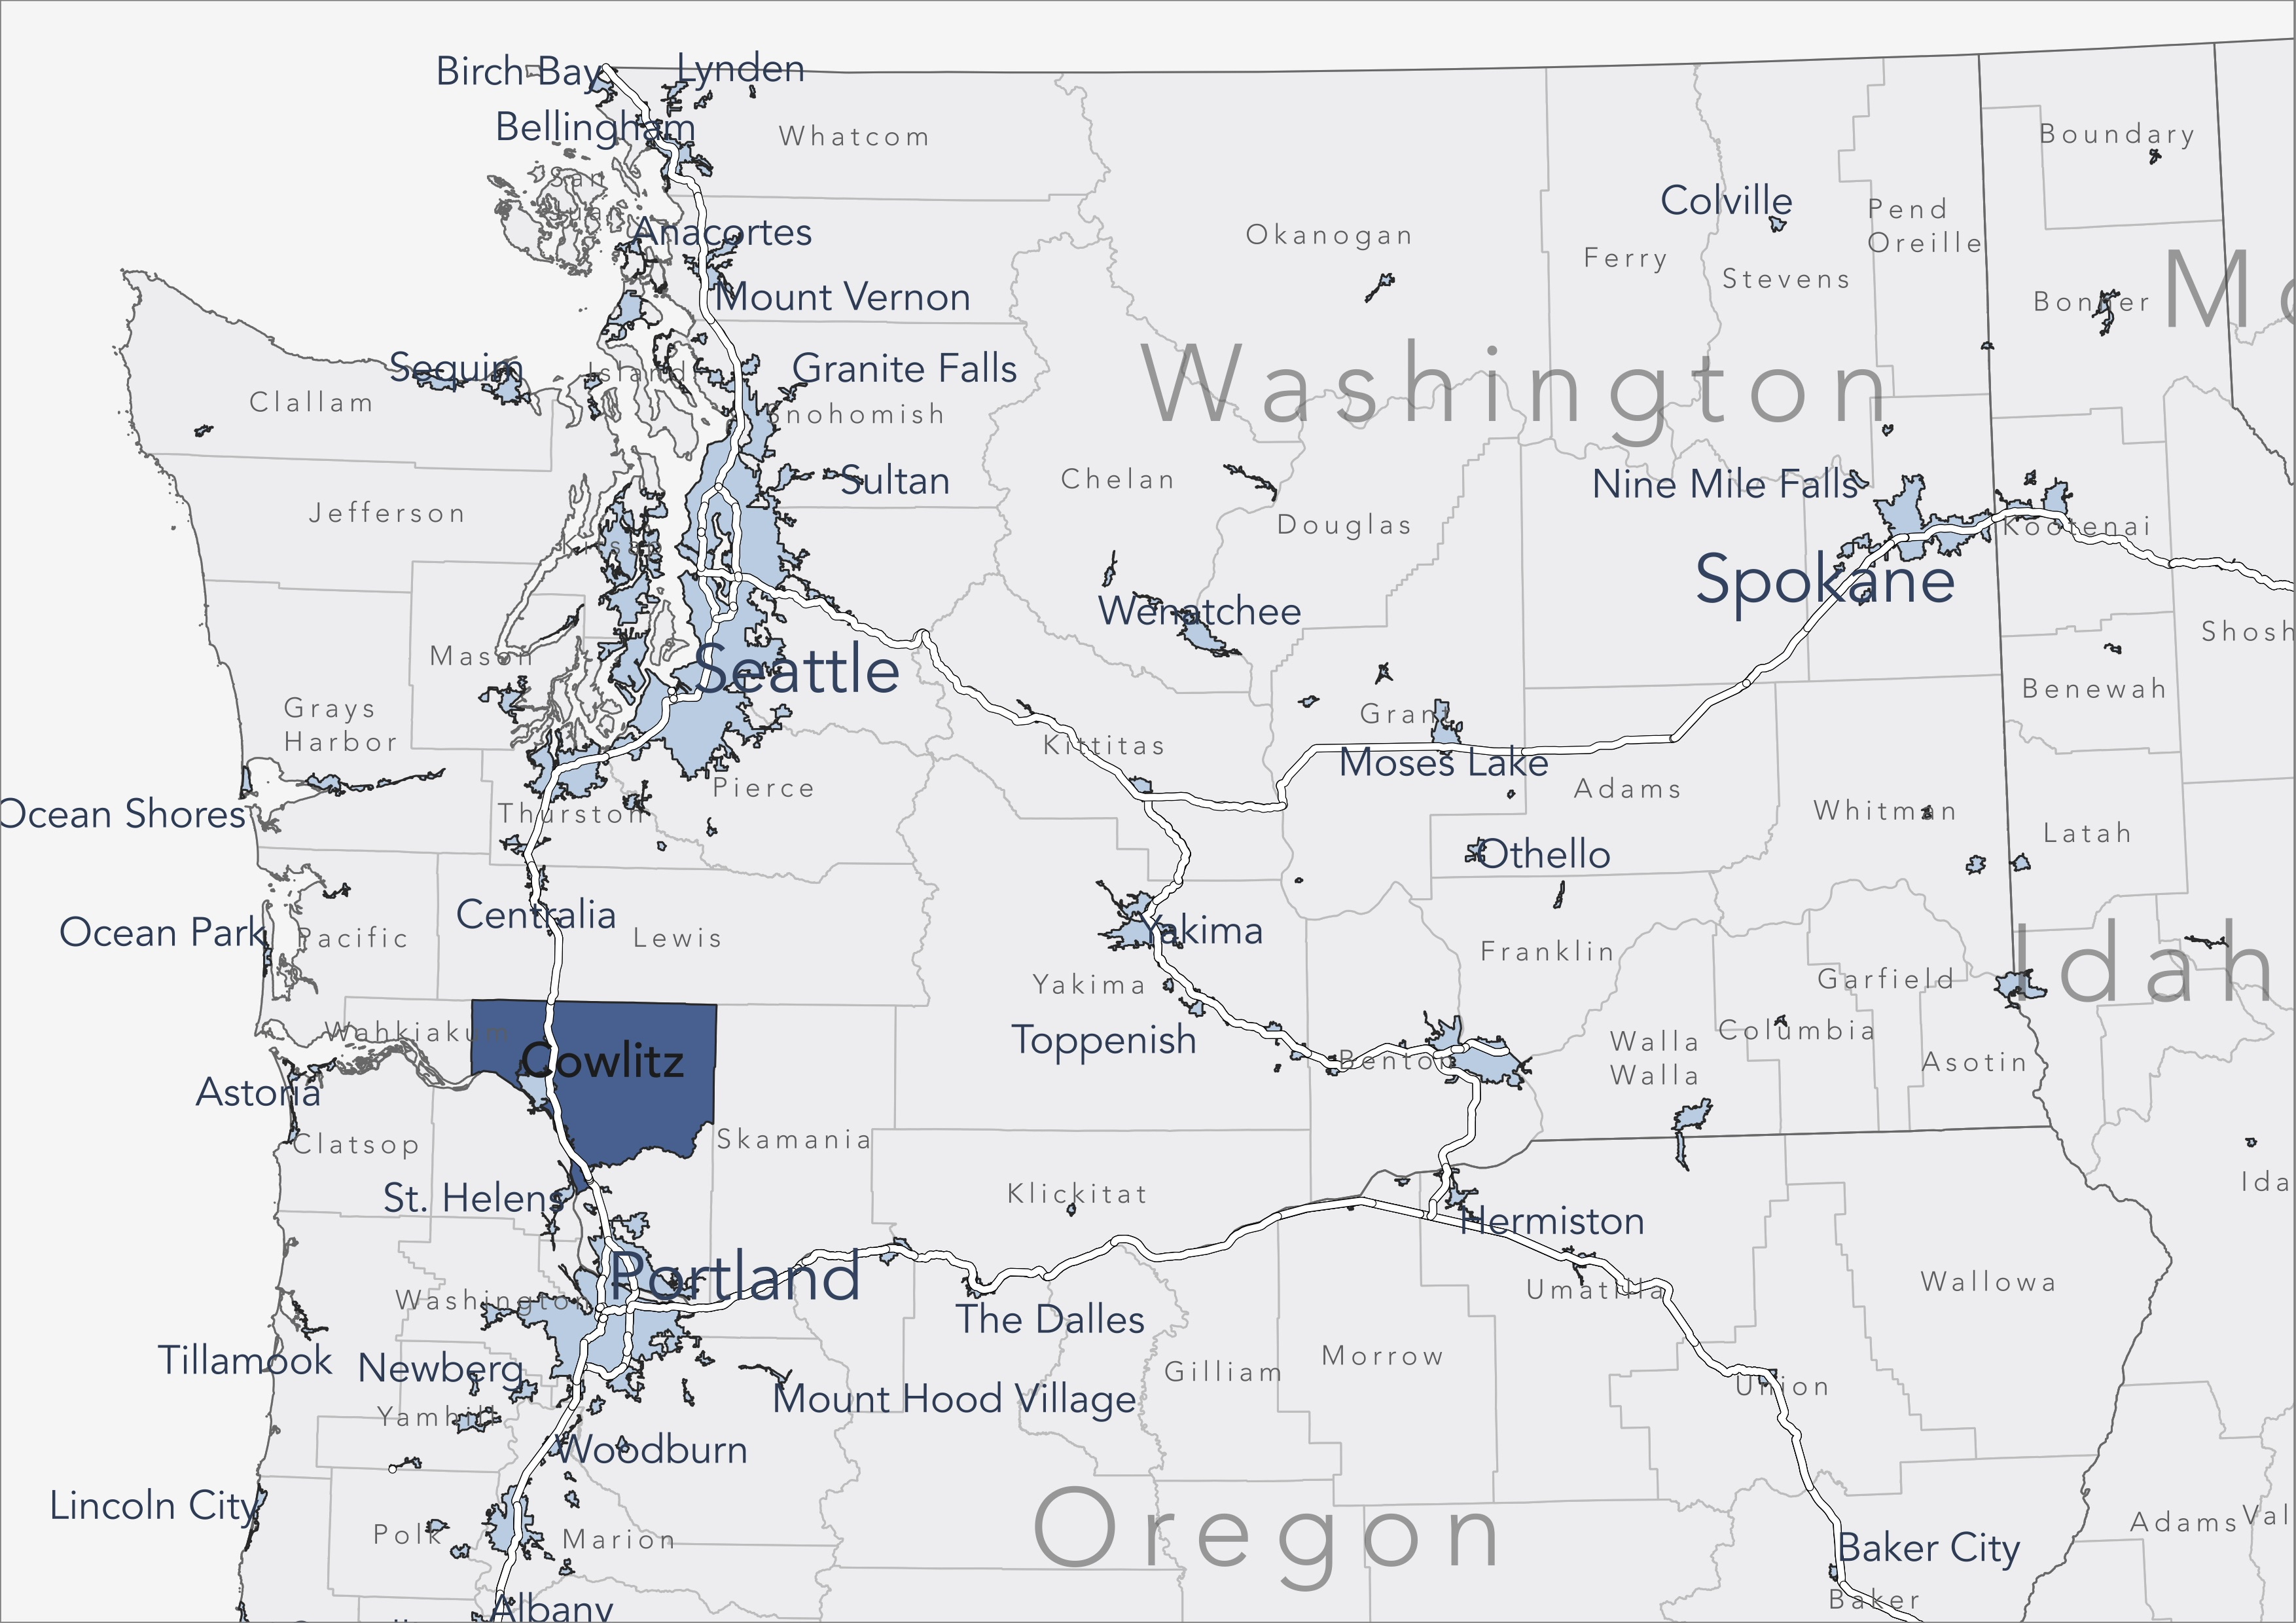
\includegraphics[angle=90, origin=c, width = 5.75in]{Figures/other_figures/Cowlitz_Context_small.jpg}
    \caption{Cowlitz County, Washington and its position in the Pacific Northwest}
    \label{fig:map_of_cowlitz_big}
\end{figure*}

\begin{figure*}[p]
    \centering
    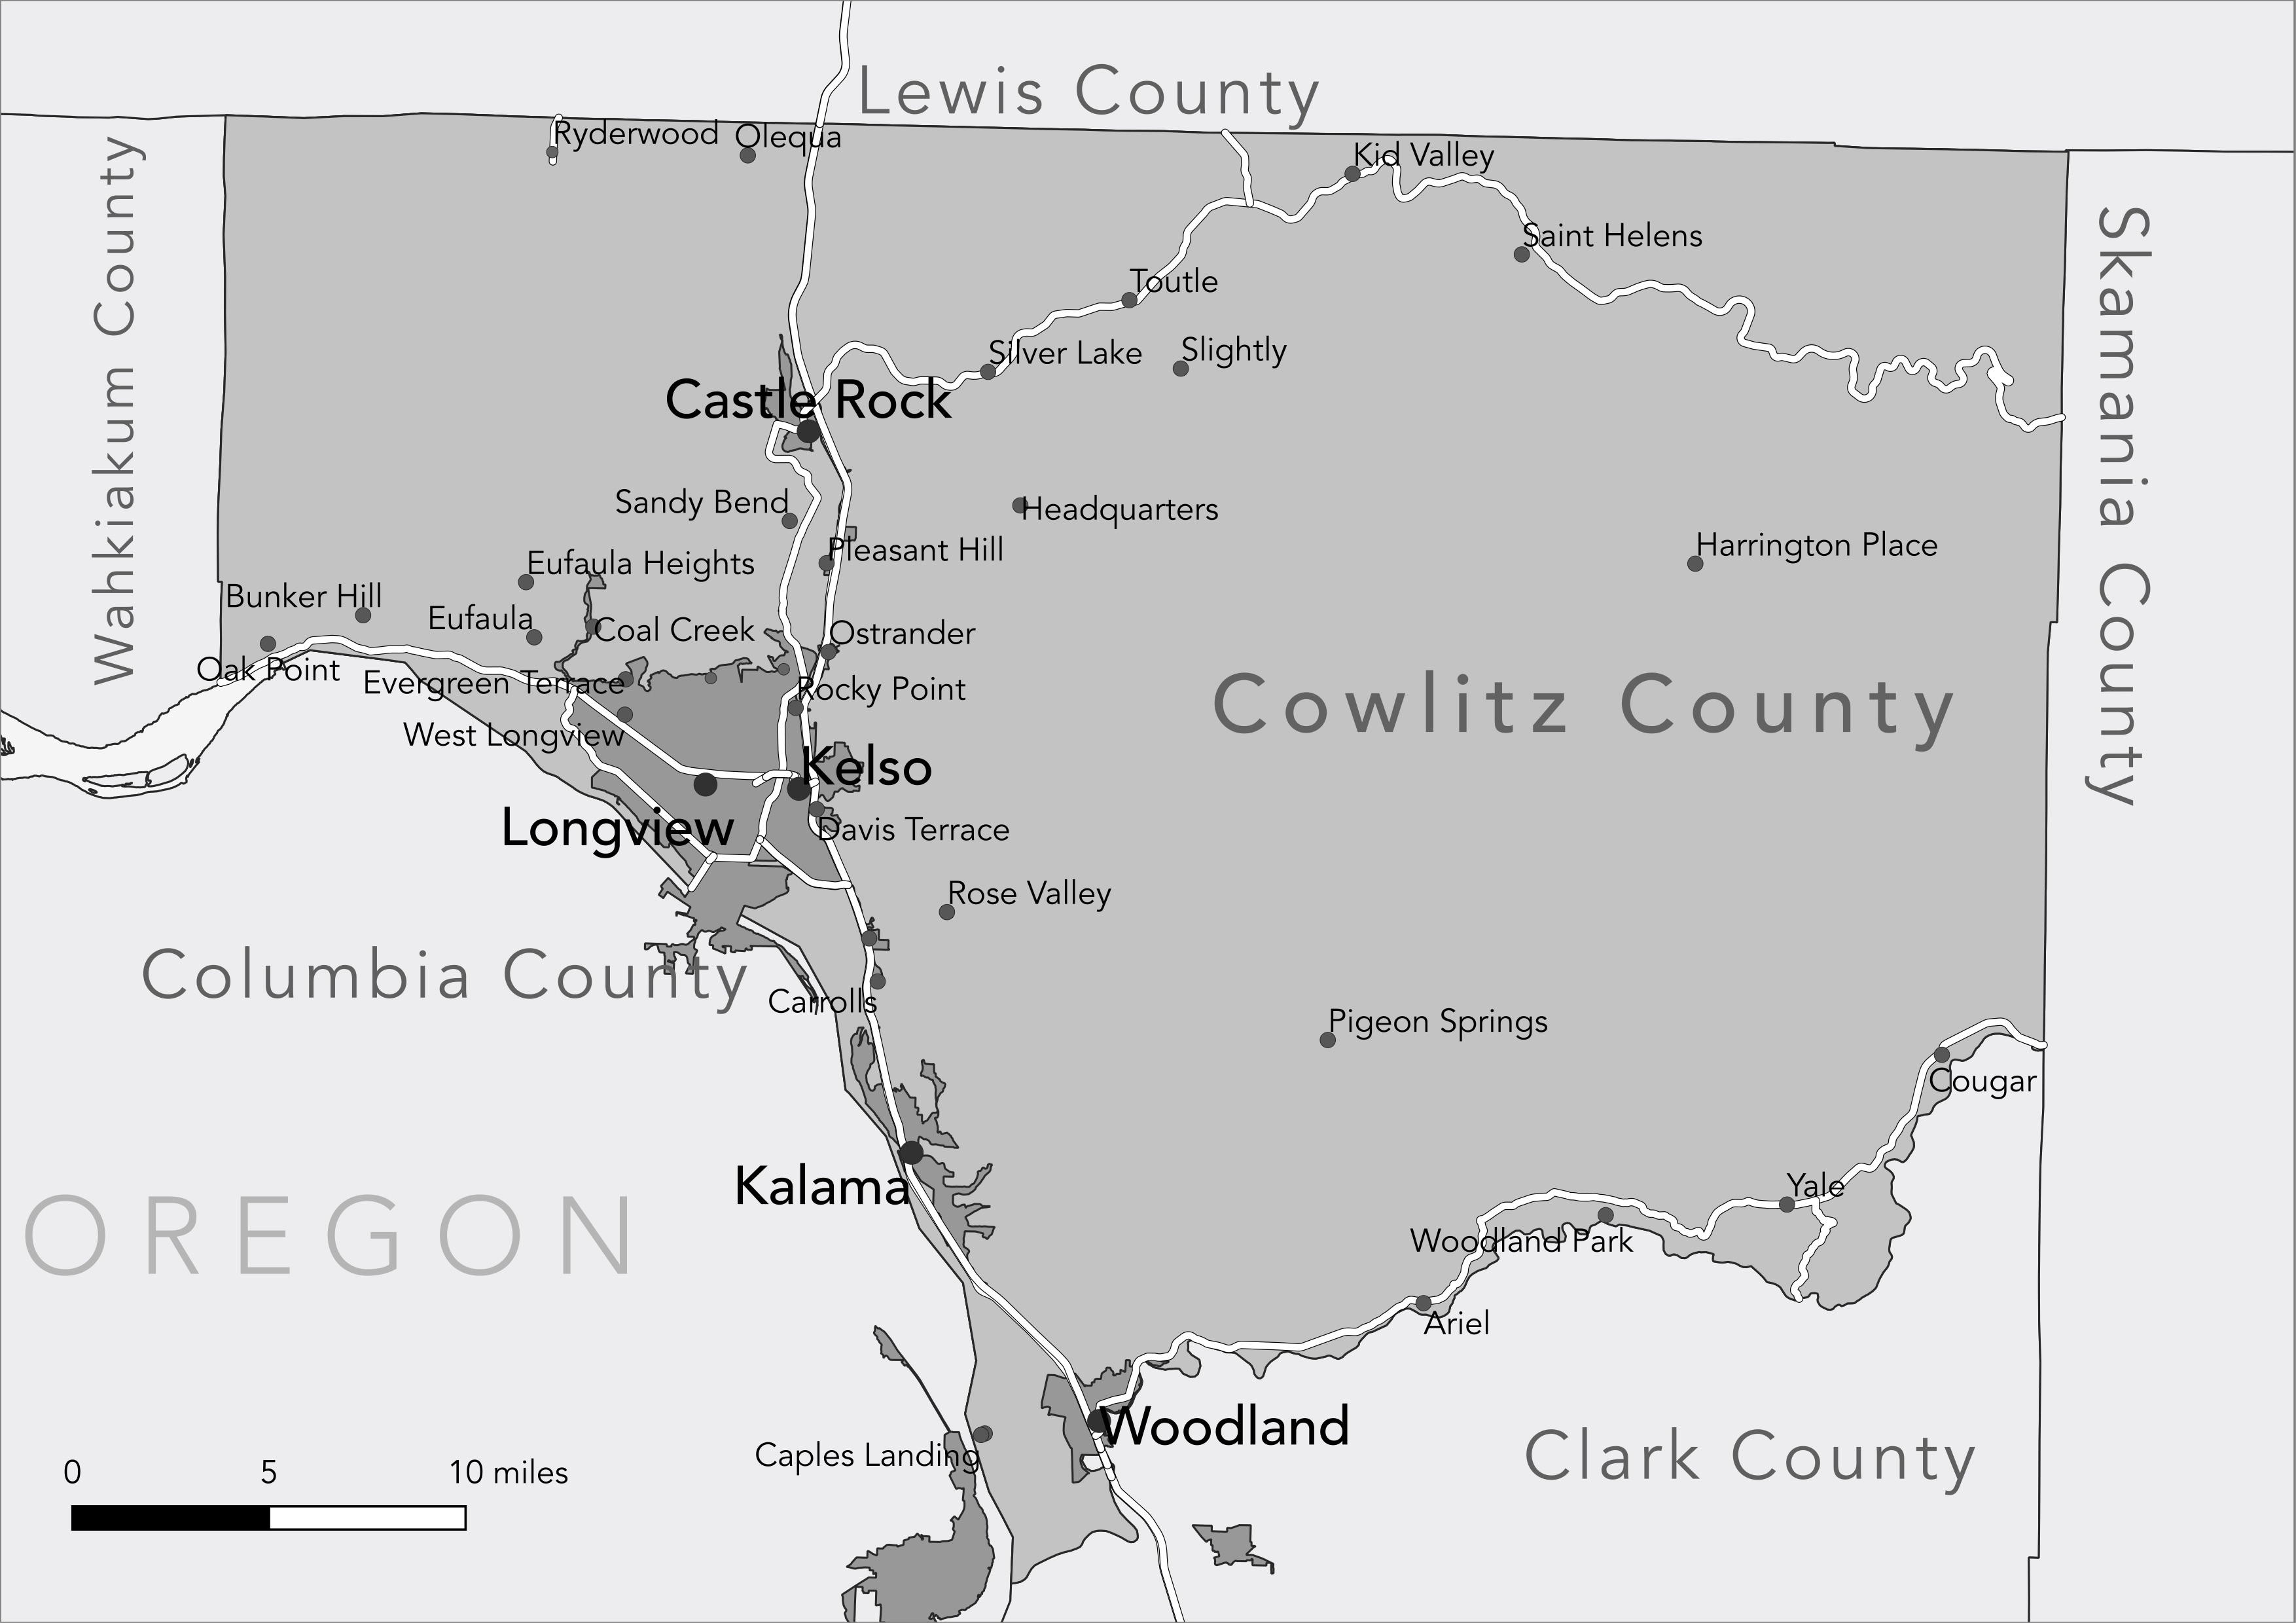
\includegraphics[angle=90, origin=c, width = 5.75in]{Figures/other_figures/Cowlitz_Focus_small.jpg}
    \caption{Cowlitz County, Washington}
    \label{fig:map_of_cowlitz_zoom}
\end{figure*}

Cowlitz County is an area of about 1,139 square miles in southwestern Washington (Figures \ref{fig:map_of_cowlitz_big} and \ref{fig:map_of_cowlitz_zoom}). Its southern border is defined by the Columbia and Lewis Rivers. Its eastern, western, and northern borders are defined by latitude and longitude. It is bordered by Wahkiakum County on the west, Lewis County to the north, Skamania County to the east, and Clark County to the south. Across the Columbia River into Oregon, it borders Columbia County.

Topographically, Cowlitz County is in the Puget Sound-Willamette Depression, meaning it is part of a long stretch of lowland that connects Puget Sound in northwestern Washington with Willamette Valley (as far south as Eugene) in Oregon \citep[2]{barrier_froyalde_1998}. It is located next to the Cascade Range and six major rivers flow from those mountains through Cowlitz County: Columbia, Lewis, Cowlitz, Toutle, Kalama, and Coweeman. On clear days you can see Mount Rainier, Mount St. Helens, Elk Mountain, and Mount Hood. However, such days are rare as rain and cloudy skies are the dominant weather patterns for eight months of the year\footnote{Weather data is taken from WeatherSpark.com.}. The warmest month is August, with an average high temperature of 79\degree F, while the coldest month is January, with an average low temperature of 35\degree F. These moderate climate makes it quite a pleasant place to live. The terrain is rather hilly and large trees (Douglass Fir and many others) cover the area.

The county is home to 102,410 people, putting the population density at 89.9 people per square mile. The five cities in Cowlitz County, with their 2017 estimated populations \citep{census_factfinder} are Longview (36,740), Kelso (11,864), Woodland (5,765), Castle Rock (2,899), and Kalama (2,497). There are an additional 31 unincorporated communities; of them, Carrols, Coal Creek, Oak Point, Ostrander, Rose Valley, Sandy Bend, Stella, and Toutle were mentioned in interviews and have historical significance. Ranier, Oregon shares a border with Cowlitz County is accessible from Longview by bridge. Other notable cities nearby include Portland (50 miles to the south), the Washington suburb of Vancouver, and Seattle (128 miles to the North) and are accessible via Interstate 5 which cuts through the county. Astoria, Oregon is 50 miles to the west and the Pacific coast is just beyond that.

As for the people themselves\footnote{County data is taken from datausa.io.}, residents of Cowlitz County are similar to the rest of Washington in that they are mostly US citizens (97.5\%) and are predominantly white (84.6\%) with Hispanics (8.4\%) forming the largest ethnic minority group. However, the median age of 41.4 is somewhat higher than the rest of the state (36.4) and appears to be increasing. The median household income was \$49,127, which is far lower than the state average of \$67,106. On average, the area is poorer and older than the rest of the state, with the majority of people working in manufacturing as opposed to the rest of the state which has more workers in the restaurant and food industry, construction, and elementary and secondary schools.

\section{The Cowlitz Indian Tribe}

The present-day region of Cowlitz County sits on the ancestral lands of the Cowlitz Indian Tribe.\footnote{According to its contemporary leaders, the official and preferred term for this people is the \textit{Cowlitz Indian Tribe}.} Relatively little is known about this peaceful people, though at one point as many as 50,000 inhabited the region between the Cascades and the mouth of the Columbia River \citep[70]{olson_1948}

Though the Cowlitz were a united group of people, they can still be classified into four primary divisions within the region \citep[8-10]{urrutia_1998}. First, the Lower Cowlitz Indian Tribe formed the largest group and settled on the lower Cowlitz and Kalama rivers. As this was an important trade route between the Columbia River, Puget Sound, and the Klikitats from east of the Cascade Mountains, they were able to garner wealth and establish a lifestyle that was more comfortable than their neighbors. The Upper Cowlitz Indian Tribe primarily lived in small villages and hunting camps along the upper Cowlitz river. Being too far upstream to rely on salmon, they took advantage of the open meadows to grow berries and rode horses to hunt game. Their proximity to Mount Rainier gave them access to trade and with Sahaptin-speaking peoples on the east side of the mountains, and after centuries of intermarriage the Upper Cowlitz spoke both Cowlitz and Sahaptin. The Lower River Cowlitz form the third group, who settled in the meadows of the Lewis River. Like the Upper Cowlitz, they were skilled horsemen. They also had extensive contact with the Klikitats, who often married into and joined Lower River Cowlitz families. The fourth group is sometimes referred to as the Mountain Cowlitz, who lived in the meadows, streams, and prairies east of the Lower Cowlitz River.

These four groups within the Cowlitz illustrate that the key to survival for in this region was adaptation and being intimately connected to nature \citep[10--14]{urrutia_1998}. To thrive in a region that includes rivers, prairies, and mountains, they were expert fisherman, gatherers, and hunters, traveling by canoe, horse, and foot. In addition to Sahaptin spoken by the Upper Cowlitz, the languages of the people were Chinook Jargon and Cowlitz, a Tsamosan language within the Salishan family \citep{lewis_etal_2016_ethnologue}.
However, their numbers declined even before those of European descent began to permanently settle the region. Disease spread throughout the area between 1832 and 1844, significantly reducing their numbers, and sometimes wiping out entire villages \citep[72]{olson_1948}. Today, the Cowlitz language is extinct and what was once a large and thriving people has been reduced to less than 200 individuals \citep{lewis_etal_2016_ethnologue}.

\section{Exploration and discovery}
\label{sec:exploration_discovery}

It is unknown how long the area that is now known as Cowlitz County has been populated. But people of European descent did not see it until October 1792. This is a relatively late date considering that extensive exploration to in Puget Sound to the north and in California to the south that had already occurred.

There were numerous close encounters by previous explorers though \citep[cf.][15-16]{urrutia_1998}. Sir Francis Drake of England, who sailed along the Pacific coast raiding Spanish in 1577, missed the mouth of the Columbia River due to thick fog. The Spanish sailor Bruno Heceta was at the mouth of the Columbia in 1775 according to his latitude, but because his men were so sick with scurvy he did not enter it. Another English seaman, Captain James Cook, saw the Columbia river between 1776 and 1780, but did not enter it because of bad weather and because he was in a hurry to get to the Strait of Juan de Fuca. Britain's John Meares of 1788 was also at the mouth of the Columbia but did not realize that the giant opening was in fact a river. Similarly, Captain George Vancouver noted in 1792 that that the color of the sea resembled a river, but he, too, was convinced that the “bay” was too large to be a river \citep[3]{olson_1948} and sailed northward to the Strait of Juan de Fuca in search of the Northwest Passage—a commercial sea route connecting the Pacific to the Atlantic.

Finally, Robert Gray, a trader and merchant, was the first to enter the Columbia river (\citealt[16]{urrutia_1998}, \citealt[3]{olson_1948}). During his first voyage, he was part of the first American crew to round Cape Horn at the southern tip of South America. Along the Pacific Coast in what is now California, Oregon, and Washington, he explored many rivers, but could not enter one because of the tide. He continued on, sailing to Hawai'i and China before returning back home to Boston via the Cape of Good Hope. On his second voyage, in search of the “Great River of the West,” he went back to explore the river he was not able to enter on his first journey. It was on May 11, 1792 that he and his crew sailed into the Columbia River, becoming the first white explorers to do so, though they traveled no further than 15 miles so they did not see present-day Cowlitz County.

Captain Vancouver, hearing of Captain Gray's entrance and wishing to claim the area for Britain, sent Lieutenant William Broughton and a small crew to explore the Columbia a few months later in October 1792 \citep[16-17]{urrutia_1998}. It was they that were the first white explorers to see the area that is now Cowlitz County, sailing inward as far as what is now Vancouver, Washington. On the way, they met the inhabitants on both sides of the river and designated names for notable features such as Mount Coffin  and Mount St. Helens.

The Lewis and Clark Expedition were also among the early explorers to see Cowlitz County, and were the first to reach the area by land rather than by sea (\citealt[20--23]{urrutia_1998}, \citealt[3--4]{olson_1948}). During November 5--6, 1805, they canoed downstream past what is now Cowlitz County, noting the villages they saw, trading with the inhabitants there, and making observations of wildlife and landmarks, such as Mount Coffin. They technically did not step foot in Cowlitz County though. The team camped on the Washington side of the Columbia river the evening of November 4 before they reached the Lewis River, just south of the present-day county line. The next evening, they camped on the Oregon side across from the Kalama river, and by nightfall November 6th they had just passed what is now the county line again and camped opposite of Wallace Island.

The land around the Columbia river was highly desirable by both the Americans and British and both sides had good arguments for why they should own the land. While Captain Gray was first to enter the Columbia River, Lieutenant Broughton of Britain went further inland. But then Lewis and Clark came to the region from the Rockies, strengthening the idea that the Americans should have the land. However, Welshman David Thompson and his small crew were the first non-indigenous people to sail the Columbia from its source all the way to the Pacific in 1811, meaning the British had a stake at the claim \citep[26]{urrutia_1998}. Both sides knew that the best way to defend a claim was to settle the area.

\section{Settlement and colonization}
\label{sec:settlement_colonization}

Because of the War of 1812, very few settlers crossed the Rockies into the area at that time, so the area of present-day Cowlitz County remained relatively free of newcomers. Part of the reason was also because the Cowlitz Tribe became increasingly hostile towards outsiders because of maltreatment by trappers \citep[31]{urrutia_1998}. This started to change in the 1830s when contention arose between Russia and the newly merged Hudson's Bay Company because of the Canadian-based company's posts in Alaska \citep[27-29]{urrutia_1998}. A deal was made, and the company could lease the land from the Russians in exchange for grains and meat. The question was where the Hudson's Bay Company was supposed to acquire these supplies. The company soon established farms in several areas, including the Cowlitz Valley, using the Cowlitz River as a passageway. Consequently, the first substantial buildings in the area were what the company called the ``Caweeman Post'': two warehouses to store grain and a house for a priest which were built in 1845 about a mile and a half from the mouth of the Cowlitz river.

However, not seeing potential in the Cowlitz or Columbia rivers, the Hudson's Bay Company soon abandoned the Caweeman Post. Before they did though, they hired two men, Joachim Thibeault and Antoine Gobin, to maintain the buildings and cattle that were left there in order to secure the land for Britain. These men joined the few other former workers of the Hudson's Bay Company who had become permanent residents of the area. Adophus Le Lewes of England settled in what is now the city of Woodland at the mouth of the Lewis River, the area where he kept cattle for the Hudson's Bay Company \citep[37]{urrutia_1998}. Quebec-born Simon Plamondon had been living there since 1838: having explored the Cowlitz River and gained favor with a Cowlitz chief, he married into the community and ended up settling in the region with his many children.

While the Hudson's Bay Company had no more interest in the area, living in the West was the dream of many Americans. The east was crowded, dirty, and in an economic depression while the West was nothing but wide open, fertile land. And as of 1850, it was free too: the Donation Land Act was passed, which promised 360 acres a person if they lived on it for four years. Once the forty-ninth parallel was officially established in 1846 as the dividing line between Canada and the United States \citep[9]{olson_1948}, Americans started coming up the Oregon trail and began to settle the area, though it took a few more years for them to come to Cowlitz County because they preferred the more fertile Willamette Valley in Oregon.

From that point, the area very quickly grew from the simple Caweeman Post to several established communities; most of today's municipalities in Cowlitz County can trace their roots to this time. Peter Crawford's claim, which was across the Cowlitz River from where Thibeault and Gobin were living, was made official on December 25, 1847. He called the area Kelso, named after his hometown in Scotland \citep[51]{olson_1948}. At that time, the three of them were the only residents for 40 miles \citep[39]{urrutia_1998}. But by 1849, there were 50 people living around the mouth of the Cowlitz river, so H. D. Huntington established the city of Monticello, named after his hometown in Indiana \citep[12]{olson_1948}. Crawford was a professional surveyor and laid out the main street of Monticello and divided the land into 1-acre lots. Meanwhile, Le Lewes was joined by family members and opened a store on his property. This encouraged others to join and by the 1850s, Woodland was a thriving community complete with a post office, a school, churches, and additional stores \citep[43-45]{urrutia_1998}. By 1850, there were over a thousand people living in the area that would become Cowlitz County \citep[68]{urrutia_1998}.

While these communities were starting to grow, they did so as a part of the Oregon Territory, a massive region created by Congress on August 14, 1848 that included all of present-day Washington, Oregon, and Idaho and parts of Montana and Wyoming \citep[10-11]{olson_1948}. This area was considered too large for a single territory, so in November 1852, delegates met in Monticello and drew up a document proposing the creation of a new territory. Congress approved the bill on February 8, 1853 and gave it the name Washington. One of the first things that was done was to make Olympia the capital and to create several new counties—one of them being Cowlitz. Thus, on April 21, 1854 , Cowlitz County was officially created: the name Cowlitz was a natural choice, and reportedly means either “capturing the medicine spirit” or “peaceful” in the Cowlitz language \citep[11]{olson_1948}.

The lumber industry has always been of primary importance in Cowlitz County \citep[85-88]{urrutia_1998}. Even the earliest settlers built sawmills to make materials for their rafts and houses. George Abernathy, an entrepreneur from New York City, saw the potential of this industry and built a sawmill at Oak Point on western edge of Cowlitz County. Using the power of Mill Creek, his mill had both a vertical and a circular saw and quickly outstripped the production of the two existing mills owned by the Hudson's Bay Company. These saws were quite lucrative for him when he could fill the demand coming from the California Gold Rush starting in 1848 \citep[18-19]{olson_1948}. Inspired by the success of the sawmill at Oak Point, many other sawmills popped up along the various rivers in Cowlitz County.

This demand for lumber only increased when steamboats began to regularly travel along the Columbia River in 1850 \citep[87-91]{urrutia_1998}. These ships burned wood to create steam, so they had to stop regularly at ports to replenish their supply. By 1853, there were five stem engines that regularly traveled from Portland to Astoria, and so communities such as Martin's Bluff and Carrolls profited from these stops by providing shops, hotels, churches, stables, post offices, and of course plenty of wood for sale. Five small communities (Stella, Bunker Hill, Midway, Nisqually, and Oak Point) thrived along a two and a half mile stretch on the west end of Cowlitz County, each with their own shops, hotels, and sawmills or log flumes. Small communities supplied resources to steamboats even on the smaller Cowlitz and Lewis rivers, even though they did not lead to major population centers \citep[99-109]{urrutia_1998}. However, with the exception of Carrolls, each of these communities faded into obscurity by 1900 when steamboats were replaced by trains.

Cowlitz County continued to enjoy a strategic position as trains began to travel the West \citep[92-98]{urrutia_1998}. The Northern Pacific Railroad company surveyed the land and eventually bought land four miles south of Carrolls in 1870 to establish a train station that would be the final stop in a transcontinental railroad. Thus, the city of Kalama was born. The population quickly grew to 3,500 as workers from all over the world built a town around the station, a town that was expected to surpass Portland in size. However, as soon as the route to Tacoma was finished by December 1873 \citep[48]{olson_1948}, Kalama floundered as Northern Pacific moved its headquarters to Tacoma. Regardless, for more than 30 years, Kalama was an important part of Cowlitz County's growth because of its location on key transportation routes. Furthermore, the establishment of trains in the area required the production of innumerable railroad ties, an industry that employed thousands, particularly up the Toutle and Lewis rivers \citep[119]{urrutia_1998}.

Starting in the 1860s, Cowlitz County was also home to a large fishing industry \citep[120-124]{urrutia_1998}. Salmon and smelt were plentiful in the area, and workers in Cowlitz County developed innovative methods of canning, preserving, and packing them to survive shipment overseas. By 1881 there were 35 salmon canaries along the Columbia river \citep[31]{olson_1948}. In the 1890s, hatcheries in Cowlitz County provided millions of Chinook salmon. However, the fishing skidded to a halt when dams were built in 1940, leaving timber as the primary industry in the area.

While logging has always been a key part of Cowlitz County, the magnitude of operations grew to an astronomical scale beginning in the 20th century Frederick Weyerhaeuser of St. Paul, Minnesota bought 900,00 acres from Northern Pacific. Then, when a massive forest fire swept through the region in 1902, it was beneficial to operate more locally, so they set up their base of operations in the small town of Yacolt in Clark County, just to the south of Cowlitz County. For 14 years they harvested the burnt trees and continued their operations until 1924. Meanwhile the mill in Ostrander specialized in cutting very long pieces of lumber (it set the world record of 240 feet in 1905; \citealt[19]{olson_1948}). During the first World War, it ran night and day to keep up with the demand, its wood often serving as posts in freight carriers in the Atlantic \citep[126-129]{urrutia_1998}.





\section{Longview: A planned city}
\label{sec:longview_a_planned_city}

Weyerhaeuser's base of operations in Yacolt was significant, but Cowlitz County was changed forever in 1918 when Robert A. Long and the Long-Bell Lumber Company decided to move from Kansas to the mouth of the Cowlitz River. Long-Bell was a successful timber company in Kansas City, but when its timber began running low, rather than retiring rich, the 68-year-old co-founder and sole-owner of Long-Bell decided to find a more suitable location for the company \citep[1]{mcclelland_1976}. To accompany their purchase of 70,000 acres of forest (containing several billion potential board feet of lumber), they bought an enormous piece of land to establish what would become the largest sawmill on the planet \citep[132-136]{urrutia_1998}. However, to prevent damage from floods, dikes were needed around the valley where the mill was; Mr. Long figured they would just buy out the rest of the valley (13,929 acres, \citealt[18]{mcclelland_1976}) at whatever price the existing settlers and farmers named. And so they did.

With such a large amount of land, Long-Bell was free to build as they suited. They estimated 3–4 thousand workers were required to operate the mill, with another ten thousand required to run a city to support those workers (\citealt[5]{wilma_2017}, \citealt[21]{mcclelland_1976}). Kelso, the newly elected county seat, had a population of 2,500 and was three miles away. Not only was this not a large enough workforce, but few of the residents had cars (and there were no roads leading from Kelso to the new mill site anyway), so an alternative solution was needed. Long-Bell decided the best course of action was to create an entirely new city, one that could support the large population needed to run the mills. Since Long-Bell owned the entire valley, they decided to plan the roads, neighborhoods, and sectors before any construction began. Rather than the untidy effects of an urban sprawl, they \textit{zoned} specific sectors for residential, commercial, and industrial use---a relatively new concept at the time \citep[22]{mcclelland_1976}. Thus, the city of Longview was born in 1923.

Long-Bell had two main goals when starting its city. First, it had to establish the mills. This goal was met less than a year later when they built the two largest sawmills in the world which would soon produce nearly two million board feet of lumber a day. The second priority was to make Longview beautiful. For example, buildings in the main business district could only be built of masonry and had to be at least two stories tall so that they provided grand but harmonious store fronts \citep[27]{mcclelland_1976}. But because the city was zoned, it grew in an unusual patchwork pattern rather than radially from a city center, meaning the roads were paved but largely empty. So Long-Bell built a large six-story hotel, the Monticello Hotel, to attract newcomers to the city. Long himself donated \$1 million to build the library, a high school, and to improve the main church. The company achieved these two goals, and the Longview attracted workers from across the country.

While Longview may have looked impressive, but there were some some aspects of its design that clearly show that the priority was Long-Bell rather than Longview's residents \citep[28--30]{mcclelland_1976}. In the spirit of making the city look nice, many vacant lots were beautifully landscaped; however a playground would not be built for another four years and no sports centers were planned. The waterfront properties were zoned for industrial use because of easy access to the river rather than for housing. (Perhaps their thought was ``Who would want to have a view of the river when our city is so beautiful?'') An imposing train depot was built, yet there was no thought for how people would enter the city by car, other than through Kelso's downtown district. The first residential areas to be developed were close to the mills, but far from the rest of town, forcing the many families without cars to walk the approximately 10 block to shopping centers, schools, and entertainment. All original homes were demolished and rather than naming roads after the original farmers\footnote{In fact, the only nod to any previous people was in the name of the Monticello Hotel. It was named after the city of Monticello which was completely erased once Long-Bell bought out the valley.}---let alone the Cowlitz Indian Tribe---the company's top executives' names were used instead.

In spite of its flaws, a massive influx of workers came to Longview, bringing with them additional manufacturers to Cowlitz County. Weyerhaeuser, with its enormous stockpiles of burnt logs,\footnote{Recall that at this point Weyerhaueser was based in Yacolt to harvest burnt logs from the forest fire in 1902.} constructed three mills adjacent to Long-Bell in 1927 \citep[161-162]{urrutia_1998}. Both of these plants produced an inordinate amount of sawdust and wood chips  which people could burn in their home furnaces. As was typical of that time however, the excess was burned in an enormous wigwam or teepee burner. Wishing to capitalize on the sawdust, Longview Fibre Company was founded in 1927 and began converting all the wood waste from Weyerhaeuser into paper products (\citealt[164--165]{urrutia_1998}, \citealt[11-13]{olson_1948}). A few years later, Reynolds Metal Company was established in 1941 \citep[175]{urrutia_1998}. By 1927, the population of Longview proper had grown to 11,600 \citep[36]{wilma_2017} and together with Long-Bell, these three companies employed several thousand in Cowlitz County.

In terms of place of birth, what was the population of Cowlitz County like at this time? Census records indicate that at least 31,914 individuals were living in Cowlitz County in 1930.\footnote{I obtained these census records using \textit{Family Search} (familysearch.org), a genealogical site owned by the Church of Jesus Christ of Latter-day Saints. I was not able to search by county of residence, so I searched for people living in Longview in 1930, which returned many thousands of records of people living in or near Longview. Data included years, states, and countries of birth and the city and county of residence. Those who lived in another county were excluded. These records are not normally available to download in bulk but I was able to save them in groups of 75 entries at a time. These hundreds of spreadsheets were then combined and analyzed in R.} Figure \ref{fig:census1930} shows that the majority of those living in Cowlitz County who were before 1930 were not from Washington but were in fact from elsewhere in the United States. In fact, even including the many children born after Longview was founded, a full 60\% of 1930 Cowlitz County were nonnatives to Washington.

\begin{figure*}[t!]
    \centering
    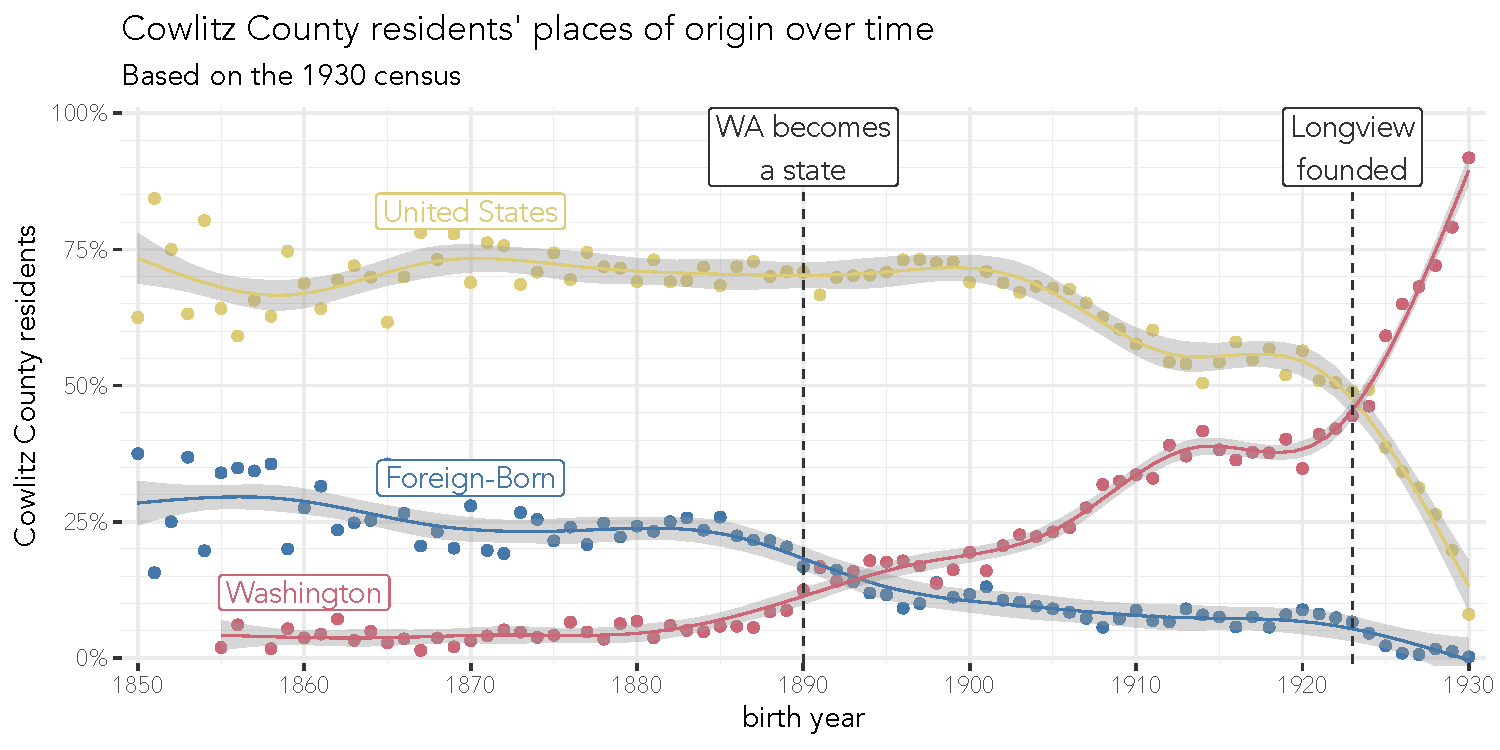
\includegraphics[width = 6.5in]{Figures/other_figures/origin_1930.pdf}
    \caption[Proportion of Cowlitz County residents by year of birth by origin ]{Given the residents living in Cowlitz County in 1930, this chart shows the proportion of origin by year of birth. The 86 octogenarians and five nonagenarians are excluded from this plot since there were so few of them and their averages were so haphazard (the data begins to fan out towards the left of the plot with those born in the 1850s).}
    \label{fig:census1930}
\end{figure*}

A closer look at Figure \ref{fig:census1930} reveals that significant events in the area correlated with demographic shifts. The proportion of foreign-born immigrants in Cowlitz County was actually at its highest all-time high in 1850 and steadily decreased over the decades. There is a small rise in foreign-born immigrants the early 1920s around the time Long-Bell was established, but this fell quickly to near 0\% by 1925. Meanwhile the proportion of people born in Washington (or the area that became Washington) in Cowlitz County has accelerated since the 1850s. They surpassed the foreign-born immigrants around the time Washington became a state and then overtook the non-Washingtonians soon after Longview was founded.

\begin{table}[ht]
    \caption[Number of foreign-born immigrants by country living in Cowlitz County in 1930.]{Number of foreign-born immigrants by country living in Cowlitz County in 1930. The 77 countries that contributed to less than 1\% of the total foreign-born population (36 or fewer people) are excluded. There were 441 people from these excluded countries.}
    \centering
    \liningnums{
        \begin{tabular}{l r r}
            Country     & People & \shortstack{Percent\\(of foreign-born)}\\
            \hline
            Canada      & 1186 & 30.81\%\\
            Finland     &  459 & 11.93\%\\
            Sweden      &  412 & 10.70\%\\
            Norway      &  296 &  7.69\%\\
            England     &  252 &  6.55\%\\
            Germany     &  233 &  6.05\%\\
            Russia      &   94 &  2.44\%\\
            Denmark     &   88 &  2.29\%\\
            Scotland    &   78 &  2.03\%\\
            Switzerland &   59 &  1.53\%\\
            Austria     &   58 &  1.51\%\\
            Ireland     &   57 &  1.48\%\\
            Holland     &   48 &  1.25\%\\
            Poland      &   47 &  1.22\%\\
            Japan       &   41 &  1.07\%
        \end{tabular}
    }
    \label{tab:foreign_born}
\end{table}

\begin{table}[ht]
    \centering
    \liningnums{
        \begin{tabular}{l r r}
            State     & People & \shortstack{Percent\\(of non-Washingtonians)}\\
            \hline
            Oregon       & 3329 & 17.27\%\\
            Minnesota    & 1289 &  6.69\%\\
            Missouri     & 1144 &  5.93\%\\
            Iowa         & 1124 &  5.83\%\\
            Wisconsin    & 1023 &  5.31\%\\
            Kansas       &  904 &  4.69\%\\
            Illinois     &  843 &  4.37\%\\
            Idaho        &  829 &  4.30\%\\
            Montana      &  787 &  4.08\%\\
            Michigan     &  723 &  3.75\%\\
            Nebraska     &  637 &  3.30\%\\
            California   &  545 &  2.83\%\\
            North Dakota &  481 &  2.49\%\\
            Ohio         &  447 &  2.32\%\\
            Indiana      &  445 &  2.31\%\\
            Texas        &  423 &  2.19\%\\
            Colorado     &  391 &  2.03\%
        \end{tabular}
    }
    \caption[Number of non-Washingtonians by state living in Cowlitz County in 1930.]{Number of non-Washingtonians by state living in Cowlitz County in 1930. Only states that contributed to more than 2\% of the total non-Washingtonian population are included here, but all US states were represented in this community. There were 1250 people from the other states.}
    \label{tab:non_washingtonians}
\end{table}

Regarding the non-Washingtonians, the majority come from northern Europe and other northern states. For the foreign-born immigrants, a full 30\% came from Canada, and the majority the rest came from areas such as Scandinavia, Finland, the United Kingdom, and Russia (see Table \ref{tab:foreign_born}). Among the Americans, it comes as no surprise that Oregon is the most represented, given that Cowlitz County is on its border. Many other people came from states now part of the Northern dialect region (Minnesota, Wisconsin, Michigan) or the Midlands (Missouri, Iowa, Kansas, Illinois, etc.). There were very few southerners, New Englanders, and a relatively small proportion of 1930 Cowlitz County came from California.

The Great Depression affected Cowlitz County like the rest of the nation, but despite nearly going bankrupt themselves, Long-Bell, Weyerhaeuser, and Longview Fibre managed to provide many jobs for the community. Part of this had to do with changes in how goods were transported: shippers discovered that it was lighter and cheaper to use corrugated paperboard rather than wooden crates \citep[69]{wilma_2017}, meaning there was an increased demand for paper products. The mills were also flexible in what products they could provide to their clients and producing new items created more jobs. To save on costs though, workers were paid less and could only work every other day, but the unemployment rate was not as high as it was in other parts of the country \citep[167]{urrutia_1998}.

Fear struck the community during the Second World War, but business was still booming. The wartime demand of lumber, paper products, and aluminum kept the manufacturing plants running non-stop, and the debts they incurred during the Great Depression were quickly paid off. Women had always worked in the mills, but around this time they began to take up the manual labor positions formally reserved for men \citep[132]{wilma_2017}. There was also an influx of loggers from California, unemployed due to heavy snow, to help the most pressing need of workers in the forests. More than ever, the mills played an important role for a large proportion of the residents in Cowlitz County.
Into the 1950s, the mills continued to thrive as consumers demanded more paper products. Much of this had to with the new ways that paper was being used. As mentioned previously, shippers switched to paper-based boxes instead of wooden crates, but items such as specialized boxes, such as for clothing or cakes, were being used more and more. Various kinds of paper were manufactured that included items like gift wrap, butchers' paper, and the little sheets of paper between slices of cheese or meat. In addition to paper grocery bags, Longview Fibre was producing special bags made for garments, poultry, nails, popcorn, sugar, and raisins \citep[122-123]{wilma_2017}.

The culture of these companies was to make sure its employees were treated right, though part of this may have been out of obligation and fear of the labor unions. In the early 20th century, unions among loggers in the Pacific Northwest were increasingly popular and grew more powerful, so fair treatment was the best way to avoid confrontation \citep[145]{urrutia_1998}. But the Longview companies went above and beyond what other sawmills did in the Pacific Northwest. Rather than muddy tents for the loggers in the forest, Long-Bell built the small city of Ryderwood, which included family homes, a store, a school, a doctor's office, and a train that took workers to and from Longview. The neighborhoods known today as the Highlands and St. Helen's were filled with modest homes for employees and their families, who could easily afford them with the stable income they brought home. Longview Fibre was concerned about the employees who had to pay the \$1 toll to cross the Columbia River into Longview, so the company used its tug boats to ferry workers over for free \citep[102]{wilma_2017}. If an injury prevented an employee from working, they continued to get their paycheck. This tradition of treating its employees well continued for decades, and as will be shown hereafter, may have set the stage for the sudden language change experienced in the 1970s.

Many of the employees in Longview's mills began work while they were still in high school. They mostly worked in the lowest-wage positions and required little training \citep[133]{wilma_2017}, but they could move their way up after graduation. In fact, Cowlitz County very quickly established the Lower Columbia Junior College in 1934 to provide courses and training in forestry and paper-making \citep[173-174]{urrutia_1998}. Employees' children often worked at the mills as soon as they were old enough to, promoting the idea of it being a family industry.

Working at Longview Fibre always meant there was a possibility of promotion. New hires almost always started at the bottom, but rather than bringing in outside hires to fill middle- and upper-level management, these spots were filled from within the company itself. One worker, Delos Wilma, began his career in 1940 unloading railroad cars and piling wood on steel cars, but retired 42 years later as superintendent of the paper mill \citep[105]{wilma_2017}. Another, Meade Cobb, started part-time while still a high schooler, but ended up as the head of the stereotype department after nearly 40 years \citep[133]{wilma_2017}. This continued until present-day: I was fortunate to interview Rich who tells of his experience in moving up the ladder within the company:
\begin{num_quote}
    "[I] joined with a company- a local company, Longview Fibre Company, as an entry-level designer. So I basically came back to my hometown to start my career. And then went on for twenty-eight years, got a few promotions and… So my job at, uh, Longview Fibre went well and the design and the engineering and I was, uh, at some point the chief engineer and then I- I got a- a step above that.\footnote{Rich is being modest here: he was a former vice president.}" (Rich, M, b. 1956)
    \label{quote:moving_up_coorporate_ladder}
\end{num_quote}
This culture of internal promotion gave workers a sense of belonging and the companies held ceremonies honoring those who worked there for many years. This culture, together with a stable and growing paycheck and a retirement package available to workers as early as 55 years old, was motivation to stay with the company.

During these years of growth in Longview, Kelso was suffering from a bit of an inferiority complex. The 70-year-old city was feeling some resentment from the new city across the river. At first, the rivalry was playful: Kelso girls would boast when they had dates with Longview boys and the football teams in the two cities became arch-rivals. But when increased traffic warranted building another bridge across the Cowlitz River, the antagonism between the two cities escalated \citep[154-155]{urrutia_1998}. Kelso made plans for a bridge connecting south Kelso to downtown Longview, but Longview's plan was to build one nearer to the mouth of the Cowlitz River, connecting Pacific Highway---the only road from Portland to Seattle—to the mills. Longview's plan won out, and in 1926 when the Pioneer Bridge was built, it completely bypassed Kelso. The traffic on Pacific Highway that used to go straight through Kelso's shopping district was diverted into Longview. Consequently, many Kelso businesses moved across the river into Longview, fueling the rivalry between the two cities. Though Kelso and Longview were only divided on a river, they developed “two cultures” \citep[xi]{wilma_2017} as a result of this animosity.

Fortunately, this hostility appears to have calmed down to merely being playful again. Cooperation finally led to the formation of the Greater Longview-Kelso Community Council and they built the Peter Crawford-Cowlitz Way Bridge in 1952. Megan \ref{quote:kelso_depends_on_longview} realizes that both cities exist because of the other:
\begin{num_quote}
    Kelso would have shriveled up and died without the airport and the train station and also the interstate… Even with that it would've just been a teeny tiny town that nobody would've ever heard of and didn't have anything. Except Robert A. Long came and made Longview a spot on the map… So, without Robert A. Long and Longview, Kelso would have died out. So, since I understand that, I'm okay now. But yeah in high school it was totally- I had my church friends who were from Longview, so it didn't really matter as much to me. But it was still like a- every time Kelso or one of the Longview schools play against each other I expect Kelso to beat Longview and I'm thoroughly disappointed if that doesn't happen. (Megan, F, b. 1992)
    \label{quote:kelso_depends_on_longview}
\end{num_quote}
Rob \ref{quote:not_gonna_happen} also mentions the rivalry between Kelso and Longview and explains that while it has calmed down, it still exists somewhat in the community.
\begin{num_quote}
\textit{Have you noticed any animosity between people from Longview and people from Kelso?}

Oh, from the day I was born, yeah. Just the city rivalry type thing. And the football teams would play each other every year the basketball teams and, y'know, it- it was just one of those things and it- it was a big deal for the people of the area to be combative somewhat. And sometimes it got out of hand, sometimes it didn't. But the- that's why the two towns could never combine. Every time you talk about combining, uh, no no, uh, too many people would have hard feelings and say, ``Not gonna happen.'' Never has. (Rob, M, b. 1942)
\label{quote:not_gonna_happen}
\end{num_quote}
This rivalry does not appear to have manifested itself linguistically in the community, but it helps describe the culture one might find among the long-term residents in Cowlitz County.






\section{The rise and fall of the mills}
\label{sec:rise_and_fall}

As described in the previous section, the mills in Cowlitz County were an integral part of the community. They were flexible enough to take advantage of changes in the economy and could recover from devastating blows like the Great Depression or the Columbus Day Storm.\footnote{Columbus Day Storm was October 12, 1962. In reality it was more than a storm and was an ``extra-tropical cyclone originating in the North Pacific'' \citep[185]{wilma_2017}. Winds reached up to 80 miles per hour, much of Cowlitz County was without power for a week, and forty-six people died with hundreds other injured. In addition to the devastating property damage within the county, the storm damaged hundreds of thousands of acres of forest owned by Cowlitz County companies. Fortunately, these fallen trees could be salvaged over the next couple of years, and the products that could be made from them were highly desirable in Japan at the time.} And their significance was not limited to their local communities: Long-Bell, Weyerhaeuser, and Longview Fibre were known regionally, nationally, and across the world. However, in as early as the 1960s, some seeds were being planted that would eventually bring the businesses down, effectively transforming the culture of Cowlitz County from a milling community to something else entirely.

Even though Longview was created because of Long-Bell, their importance on the community decreased over time. Technology advanced, and as cars became more affordable, people could live further from Longview. This made the community less centralized and it diminished the importance of the mills as the primary cultural hub of town. Meanwhile, the demand for paper was as high as ever, and larger paper companies gobbled up smaller ones at this time. For example, Weyerhaeuser expanded to the pulp and paper industry in 1964. Long-Bell was not so well off, and when they merged with International Paper in 1965, they demolished their two massive sawmills to accommodate the new machinery. As a testament to the decentralization of the mills in Longview, one only need to compare the city's reactions to Long-Bell's first and last days. On July 24, 1924 when the first log was loaded onto the headrig, the entire city celebrated with a 4-day pageant that included parades, a rodeo, and a circus \citep[144]{urrutia_1998}. Forty years and 8.7 billion board feet later when the last log went though, Urrutia explains that ``[t]he city of Longview, completely cut off from the apron strings of the founding company, by that time had enjoyed such independence from being thought of as a company town that it scarcely took note of the demise of its parent'' \citeyear[188]{urrutia_1998}. The mills were still among the largest employers in the county, but they were seen simply as a place of work rather than part of the town's identity.

Early 20th century labor unions, as described in the previous section, made sure that mill workers were treated well. However, starting in 1967, these unions—more organized and larger than before—began negotiations with the employers after several years of intermittent strikes \citep[196-198]{wilma_2017}. While this was going on, inflation was increasing faster than ever in the early 1970s, and this of course had an effect at in every part of the business from buying materials, selling costs, and salaries. Employees were demanding raises as high as 10\% a year, and companies like Longview Fibre could not keep up. There was an energy crisis in 1973 and a slump in the number of homes being constructed in 1974 which reduced the amount of timber that could be sold \citep[218]{wilma_2017}. New environmental laws around this time also cut into companies' profits as they had to spend millions on treatment systems.

The pivotal year was 1977. The mills were struggling already after several years of lower production due to strikes and wage increases. But when the price of oil went up, meaning shipments to Japan were costing more and more, companies could not keep up with wage increases. Employees at mills all across the Pacific Northwest were going on strikes and approximately ten thousand workers walked. In Longview, there was hostility towards salaried employees and executives who did continue to work, and while most of it was nonviolent, there were minor incidents such as slashing car tires \citep[200-202]{wilma_2017}. These strikes continued for several years.

As a result of this and other outside forces, the 1980s was a rough time for the timber industry in Cowlitz County. The number of employees working involved in the mills and other timber-related production peaked at 12,210 in 1977 in Cowlitz County and steadily declined since then. Though the companies were still mostly profitable, their impact on the community and the number of jobs they provided was decreasing every year. Longview Fibre went into debt for the first time—by \$113.9 million—in 1981. This marked a clear beginning to its downfall that would eventually lead to their being bought out in 2007. The companies were still loyal to their employees as much as they could be, continuing to pay dividends to stockholders and keeping as many jobs as possible. The state of Washington as a whole was hit hard by the national recession in the early 1980s, but unemployment in Cowlitz County soared, far above even the state average, to 17.5\% at that time. The eruption of Mount St. Helens in 1980 may not have had a significant long-term effect, but it exacerbated the increasing problems in the area at least for a short while.\footnote{Mount St. Helens, a volcano just 36 miles due east of Longview as the crow files, erupted in May of 1980. The direction of the explosion was northward and the winds blew east, so Longview only saw a few centimeters of ash. However, closer to the volcano, this ash made logging in the woods far more difficult as it quickly wore down the chainsaws. Not only were thousands of acres of timber destroyed, but the Cowlitz River flooded with mud, causing evacuations in some areas. It was also full from shore-to-shore of downed timber, causing destruction of property as it hurled these giant trees along at 60mph. In my interviews, I was fortunate to hear many first-hand stories of life in the months after Mount St. Helens blew.} The price of raw goods skyrocketed, outpacing inflation, meaning companies made less and less profit \citep[268]{wilma_2017}. Many companies were moving manufacturing plants offshore, further reducing the number of jobs available to local residents.

This sudden change in town was observed by its residents. Carol \ref{quote:mt_st_helens}, who had several family members lose their jobs in the early 1980s, says this about the changing community:
\begin{num_quote}
    "There were a lot of people that worked in the woods, and if they didn't work in the woods they were like support system, like office people\ldots A lot of people lost their jobs and a lot of people moved. A lot of people just got out of here. And so you take that kind of income from these people out in the woods—and they made really good money considering, y'know—okay, so what does that do to the rest of your economy? They're no longer buying as much gas. They can't afford to go out and go to the movies and eat out and groceries… So yeah. It hit us especially hard." (Carol, F, b. 1958).
\label{quote:mt_st_helens}
\end{num_quote}
Similarly, Teresa points out the increased difficulty in finding jobs affected the culture of the area:
\begin{num_quote}
    ``[In the 1960s and 1970s,] it probably felt more rural or more isolated because people didn't really move away that much then. You know what I'm saying, people were just here, they expected- a lot of guys expected just to go get jobs in the mills and that started changing of course in the eighties. So um so my generation's probably the last generation that got grandfathered into their jobs. So, so that has changed and also our community has changed since that time. Yeah, it's cuz those jobs aren't available anymore, so.'' (Teresa, F, b. 1956)
\label{quote:changed_culture}
\end{num_quote}
Throughout most of the 1980s, the population of Cowlitz County increased because births outnumbered deaths, but more people left than there were immigrants into town. It took until 1987 for the unemployment rate in Cowlitz County to fall below 10\% again.

People also commented on changes within the companies. The mills used to be considered family companies and places where it was easy to get jobs, even while still in high school. But Bruce \ref{quote:easy_To_find_work}, who comes from a family of loggers, noted the difficulty that people have in getting jobs recently:
\begin{num_quote}
    "Back then, everybody… could find work. Y'know somebody had a job say, ‘Hey there's an opening. Come in.' And it's who you know. And go right to work. Like my dad, y'know, you just say, ‘I got a son.' Well they just hired him and went to work. Now, I hear, they don't have the degree. They don't have the knowledge to run the paper machines. So, I hear on the radio they're always advertising, ‘Okay there's a special guy to run the machinery. We don't have anybody [who's] qualified to run these new fancy machines.' So now you have to hire these college kids… Yeah so things change a lot to technology. So it's not like you can't just go in there and work so it's… everything is advanced now." (Bruce, M, b. 1958)
\label{quote:easy_To_find_work}
\end{num_quote}
Historically, people started with the unskilled jobs, there were always opportunities to move up, and middle- and upper-management positions were always filled from within. The qualification to work in management positions was simply experience within the company rather than a college degree. But Harold \ref{quote:family_company}, who worked at the mills his whole life, shares this insider's perspective about the effects of increased automation and the use of technology:
\begin{num_quote}
    "At that time [in the 1970s], it was a family company. Everybody wanted their sons to work there or their daughters to work there. And then it slowly started changing… and it started getting away from a family wage job. It started getting away from guys that knew their profession working up through the ranks so your boss knew the job. By the time I retired forty years later, all the bosses were college graduates with an engineering degree that they thought automatically could tell the guy with forty years' experience how to do the job." (Herold, M, b. 1949)
\label{quote:family_company}
\end{num_quote}
Putting it more succinctly, Ed \ref{quote:down_the_tube} simply says:
\begin{num_quote}
I grew up in good times. The sixties was a good era, the seventies was good, eighties. And then it started going down the tube. (Ed, M, b. 1949)
\label{quote:down_the_tube}
\end{num_quote}
The topic of the changing economy in the 1970s and 1980s was not mentioned by all of the interviewees and it was only during the course of data collection that I became aware of it and its impact on the community. But the fact that several of these people talked about it unprompted supports the idea that it was a significant change in the community. As a point of comparison, there were only two passing references to the recession of the late 2000s in all of the 54 interviews.

These changes had a lasting effect on the community. At its peak, manufacturing jobs accounted for 45\% of the total income in the county. Twenty years later in 1996, this dropped to 27\% and in 2015 it was approximately one-sixth of the total income. Not only are fewer people working at the mills but their salaries are lower, relative to the rest of the country. In fact, the inflation-adjusted earnings per capita peaked in 1977 at \$19,352 before falling drastically to less than \$15,926 in 1985. It took Cowlitz County twenty years to return to the level it was at in the 1970s.

Into the 2000s, Longview Fibre, one of the few successful mills in the area in the 1980s, had to reduce the variety of products it could provide to its customers. Just as new products created new jobs in its early days, cutting products meant layoffs and, consequently, less revenue coming into the community. It also had to reduce the dividends its stockholders had come to rely on. Eventually, it was bought out and fell into the hands of Kapstone in 2007. However, unlike the machines belonging to other former companies in county, Fibre's mills continue to operate, meaning there are still at least some timber-related jobs in the area.





\section{Cowlitz County today}

Summarizing its history, it is clear that Cowlitz County has had its ups and downs. Its strategic position on a transportation route allowed it to flourish during the 19th century (just as the Cowlitz Indian Tribe had before European explorers). When giant milling operations came to the area in the 1920s, the population exploded, creating the city of Longview and a thriving community where high-paying jobs were easy to acquire. But, after 50 years of plenty, these companies could not keep up with the sudden and simultaneous onslaught of new economic pressures. The industry buckled, sending the community into a 20-year recession.

Cowlitz County has never returned to the thriving community it once was. \citet{bailey_2016} reports that over the last few decades, the unemployment rate has consistently been higher than the national average. During the recession in the late 2000s, it was at one point as high as 15\% and it took until 2017 to bring it back to pre-2008 levels. The inflation-adjusted earnings per capita peaked in 1977 at \$19,352, and after falling to \$15,926 in 1985 it would take until 2000 to recover. The population was relatively stagnant through the 1980s, and Longview has never reached the goal of 50,000 that it was originally designed for.

With this background in mind, I will now present the methods and results of this study in the following chapters. The major events in the history of Cowlitz County, namely the establishment of Long-Bell in 1923 and then the subsequent decentralization of the timber industry in the 1970s and 1980s caused large demographic and attitudinal shifts in the community, shifts that correlated with changes in vowel pronunciation. Therefore, in addition to pressures from neighboring regions, I show that these local changes are linked with the Elsewhere Shift in Cowlitz County.
 % 8,135 words
\clearpage\chapter{Methodology}
\label{ch:methodology}

\begin{quote}
    I can imagine no better place than a Northwestern logging camp for a philologist to spend a summer in. Here\ldots he can earn five dollars a day, breathe mountainy air, enjoy the keen smells of the conifers, and build up the abdominal muscles for chesty logger talk while he is making his investigations. \citep[139--140]{stevens_1925}
\end{quote}

In this chapter I discuss the methods for data collection, processing, and analysis that I use in this study.\footnote{The procedures for recruitment, consent, and data analysis described in this chapter were approved by the Univeristy of Georgia Institutional Review Board on April 11, 2016. The study ID is STUDY\liningnums{00003041}.} I begin by describing my fieldwork methods in \S\ref{fieldwork}, including how participants were recruited, the interview itself, and the equipment used for recording. Next, in \S\ref{participant_metadata}, I describe the demographic metadata about the participants and provide a brief description of the participants in this study. I discuss how my data was transformed from raw audio files to spreadsheets of numbers in \S\ref{processing}, including transcription, forced alignment, formant extraction, and filtering. Then, I use \S\ref{word_classes} to explain the word classes in this study, including their labels and how they are defined. In \S\ref{corpus_size_constitution}, I describe the corpus size and constitution. Finally, I discuss the statistical analysis for this study in \S\ref{statistical_analysis}. In summary, this dissertation uses traditional techniques for data collection, standard procedures for processing, and recent developments in statistical modeling for analysis.

% --------------------------------------------------------------------
% ------------------------    Fieldwork    ---------------------------
% --------------------------------------------------------------------

\section{Fieldwork}
\label{fieldwork}

The data analyzed in this study was collected via sociolinguistic interviews. This technique is an adaption of the traditional dialectology interviews of the early 20th Century in that participants participated in a guided conversation while being recorded. However, rather than being focused on eliciting key linguistic items, the sociolinguistic interview aims to collect speech samples in a variety of styles, from casual discourse to situations where speakers pay the most attention to speech. This method is subject to some criticism (see, for example, \citealt{wolfson_1976}), but it continues to be the standard and most popular method for data collection in sociolinguistics.

\subsection{Participant recruitment}

I collected the data that is used in this dissertation during late June and most of July 2016 in Cowlitz County, Washington. Participants were recruited primarily through my family’s contacts, but I also timed the trip so that I could find potential participants at the Go Fourth Festival, an annual celebration at Lake Sacajawea around the 4th of July, and contact local organizations like the high school’s alumni association. A few participants were recruited through social media and others face-to-face, especially on the campus of Lower Columbia College in Longview. Those who were interviewed were also invited to participate in the recruitment process themselves through word of mouth or, especially in the second half of the trip, through specially designed business cards. In total, I interviewed fifty-four self-described natives of Cowlitz County, loosely defined as being born in or having spent most of their life in the area.

\subsection{The sociolinguistic interview}

The primary goal when meeting participants was to make the environment as casual and comfortable as possible. The interviews occurred at places convenient for the interviewees such as speakers’ homes (living rooms or kitchen tables), churches, and offices or in public places like a conference room in the Longview library, the student center at Lower Columbia College, and a Starbucks. Following \citet{feagin_2013}, I dressed appropriately for the age of the participants by wearing casual clothes for younger people and business casual for older participants.\footnote{\citet[37]{hall_lew_2009_diss} mentions that she made the effort to dress as consistently as possible for all the interviews, which made her more easily recognizable at community events. I felt that modifying my dress for the interviewer, particularly for the older people, was more appropriate in this community.} Because of the power asymmetry that may be present when meeting an ``expert'' researcher \citep[197]{schlling_2013}, I emphasized my status as ``just a student'', both in conversation and appearance. Specifically, I looked the part by wearing a backpack and kept my ``nothing special'' equipment\footnote{As described below, the equipment was good, but I downplayed it a little bit in front of the participants.} in a handmade bag. Additionally, I frequently mentioned my wife and newborn child to show that I was a regular person. However, I ``temporarily step[ped] into the `expert' role'' \citep[236]{schlling_2013} when presenting the consent forms and setting up recording equipment to convey to the participants that the recordings would be of good quality and that I would treat them with great care. At each location, I made efforts to reduce background noise by turning off fans, air conditioning units, ticking clocks, and, in one case, a particularly noisy refrigerator.

For roughly half of the interviews, my mother-in-law was present and played an active role as an interviewer. \citet[110]{schlling_2013} points out that it may seem counterintuitive to introduce a second interviewer because it may swing the power dynamic too far towards the interviewers; however a third person in the room eliminates the potentially uncomfortable one-on-one setting, making the interview feel more like a conversation and less like an interrogation. In the case of my mother-in-law, while she is not a native of Cowlitz County, she has lived there for over 20 years and has achieved an in-group status that I could have never obtained as a visiting researcher. Plus, she is a great conversationalist and did an exceptionally good job at getting people to talk. In other words, introducing a third party to the interviews allowed participants to be more relaxed, allowing for more natural discourse.

The format of the recording session was that of a traditional sociolinguistic interview \citep{labov_1984}. After greetings and introductions, participants signed consent forms and were briefed on the purpose of the study, though specific linguistic features were not mentioned. After consent was given, the microphone was turned on and a 35--50-minute conversation followed.\footnote{Most interviews started with something along the lines of, ``The purpose of this is to get you talking as much as possible, so feel free to go off on tangents and tell the `long version' of stories. Basically, just tell me your life story. You have 45 minutes. Go!'' I initially started this way half-jokingly, but it actually turned out to be an effective way to get people to start talking.} Conversation topics were modified from recommended questions and protocols used by \citet{wolfram_1974}, \citet{tagliamonte_2006}, and Labov \citep{labov_1998_2004, labov_1984}. However, they were supplemented to include questions that would be more relevant to this particular community, such as asking about Portland, Seattle,\footnote{I initially asked about Portland and Seattle to have something local to talk about. However, it became clear that these responses were correlated with pronunciation differences: younger people liked Portland more and had more shifted vowels. I address this further in Chapter~\ref{ch:discussion}, and, in particular, \S\ref{sec:portland_vs_seattle}.} the mills, and local natural disasters. By far the best question was to ask about experiences related to the eruption of Mount St. Helens in 1980, which turned out to be the most effective tool for eliciting narrative and natural discourse secommunity (cf. \citealt[92]{moonwomon_1991_diss} on eliciting stories about a recent earthquake in her work in San Francisco). Few participants were in any danger, but most were excited to tell their stories. Even some of the younger speakers were happy to relate their parents' stories. When the prepared questions failed to pique the informants' interests, the topic of conversation turned to their hobbies and other interests. In all cases, the interviewers spoke relatively little, and the bulk of the conversation was taken up by the informants' speech.

At the end of the conversation, participants were asked to complete several tasks in order to elicit a more careful speech style (see Appendix~\ref{appendix:reading_passages}). First, participants read a short, neutral, three-sentence passage called ``Friends'' to evaluate their reading level and comfort.\footnote{The passage was used by Labov in New York and did not target any specific features in either of our studies \citep[417]{labov_2006}.} If there were no perceived difficulties (i.e. illiteracy or vision-impairment) and if time permitted, participants were asked to read a longer passage called ``The Cat and the Mice'' \citep{freeman_2014}. This adaptation of one of Aesop's Fables was written by Alicia Wassink to specifically target features known to be variable in Washington. The subject matter of this passage was entertaining enough that participants rarely made any comment about specific words it contained, suggesting that they were likely not aware of the particular linguistic variables being studied.

To move on to an even more careful speech style, one that is used when all context is stripped out and focused on individual words, speakers then read a 160-item word list. This list was carefully crafted to elicit multiple tokens of variables that are known to currently be in flux in the Pacific Northwest (pre-velar raising, back vowel fronting, the low back merger), variables that were mentioned in \textit{Linguistic Atlas of the Pacific Northwest} but have not received as much attention in contemporary research (the \textit{hoarse-horse} merger,\footnote{Most North American English speakers merge \north with \force (\textit{i.e.} the \textit{hoarse-horse} merger), but in a few scattered dialects, the distinction between the two may be retained or \north may be merged with \start (\textit{i.e.} the \textit{cord-card} merger) \citep{labov_ash_boberg_2006_anae}. \citet[560]{reed_1961} suggests that some speakers in the Pacific Northwest do not have the \textit{hoarse-horse} merger and instead have some other configuration. None of the speakers in this sample appeared to have anything but the mainstream \textit{hoarse-horse} merger.} the \textit{Mary-merry-marry} merger, /r/-intrusion in \textit{wash}, (wh)-aspiration, and palatalization of words like \textit{dew} and \textit{Tuesday}), and a few variables not known to be variable in the region like low and back vowels before laterals \citep[cf.][]{stanley_2017_ADS} and (thr)-flapping \citep[cf.][]{stanley_2019_thr}. The words were randomized and then the order was manually adjusted where needed so that that adjacent words did not contain the same vowel. Visually, the words were displayed in a four-by-four grid, with each cell containing 10 tokens in one column, center-aligned (see Apppendix~\ref{appendix:wordlist}). Most participants read the words from top to bottom, left to right while a few read the words left to right, top to bottom. Because the list was presented as ``just a list of random words,'' participants did not appear to catch on to the specific linguistic variables or to the fact that it was an unbalanced sample of English (there were no high front vowels, and a disproportionate number of pre-lateral tokens).

After the wordlist, speakers were asked complete a minimal pair task to focus their attention on individual sounds (see Apppendix~\ref{appendix:minimal_pairs}). The list of 40 pairs and 5 minimal triplets were again carefully selected following similar criteria as the word list, except the targeted variables were potential mergers only. In addition to production data, this task elicited some intuition of the vowel classes in question: speakers were asked after each minimal pair and triplet to say whether they thought they pronounce the words the same. There were at least two pairs of words that targeted each possible merger (sometimes as a part of a minimal triplet), providing a small indication of the degree to which the pair is merged for an individual. To test speakers’ attention (since this was the final task after an hour of talking) the list included a few filler pairs are presumably homophonous for all North American English speakers (e.g. \textit{stairs} and \textit{stares}).

In some of the interviews, participants were asked to also take part in an “elicitations” task where I would ask questions that would prompt them to say specific words. The following list displays the questions that I asked with the intended token in italics.
\begin{enumerate}
    \item Could you count for me from 1 to 10? \textit{two}, \textit{six}, \textit{seven}, \textit{ten}
    \item And would you please say the days of the week? \textit{Tuesday}, \textit{Wednesday}, \textit{Saturday}
    \item Can you list as many articles of clothing as you can think of? \textit{pants}, \textit{coat}, \textit{hat}, \textit{cap}, \textit{boots}
    \item What sorts of things would people make for breakfast on a holiday or if they had family over? \textit{eggs}, \textit{toast}, \textit{juice}, \textit{coffee}, \textit{hash browns}
    \item What kinds of spices would you find in someone’s cupboard? \textit{nutmeg}, \textit{oregano}, \textit{cinnamon}
    \item What kinds of animals would you see on a farm? \textit{goat}, \textit{dog}, \textit{horse}
\end{enumerate}
This task actually proved quite effective in eliciting specific tokens in certain vowel classes. For example, there were several tokens of back vowels (\textit{two}, \textit{Tuesday}, \textit{boots}, \textit{juice}, \textit{coat}, \textit{toast}, \textit{goat}), low back vowels (\textit{dog}, \textit{coffee}), prevelars (\textit{eggs}, \textit{nutmeg}, \textit{oregano}), prenasal tokens (\textit{cinnamon}, \textit{ten}, \textit{Wednesday}, \textit{pants}), front lax vowels (\textit{six}, \textit{seven}, \textit{Saturday}, \textit{hash browns}, \textit{cap}, \textit{hat}), and a token of \north (\textit{horse}). However, I forgot to do the task for all speakers, so this data was inconsistent across the corpus. For the purposes of this study, these elicited tokens will be grouped with the conversation data.

\subsection{Equipment}

The equipment for the interviews was of sufficient enough quality for sociophonetic analysis. Most participants wore a JK MIC-J 044 lavalier microphone, positioned about a foot away from their mouths and slightly to the side, connected to a TASCAM DR-05 digital recorder at 48kHz sampling rate and 24-bit depth. Because of technical difficulties, two interviews were recorded on backup equipment:\footnote{These were used for the fourth and fifth interviews (Megan and Brandon), because the SD card in the handheld recorder was full after the first four interviews and I hadn’t yet figured out how to transfer the files to my laptop.} a Blue Yeti microphone connected to an early 2013 model MacBook Air, using Praat \citep{boersma_weenink_2018_praat} as the recording software with similar audio specifications. Interviews were recorded in WAV format and stored on a shock-resistant external hard drive dedicated to the project. No problems occurred with the equipment and no data was lost during or since fieldwork.


% --------------------------------------------------------------------
% -------------------    Participant Metadata    ---------------------
% --------------------------------------------------------------------

\section{Participant metadata}
\label{participant_metadata}

I chose to gather speaker metadata using indirect means. In other words, participants were not asked directly about their age, gender, ethnicity, socioeconomic status, or any other demographic information. However, some of this information was offered freely during the interview. For example, some participants disclosed their age or birth date during introductions at the beginning of the interview. Most others gave indirect clues, such as mentioning offhand the year they graduated from high school or how old they were during the eruption of Mount St. Helens. Together with my personal judgments, these indirect clues were used to code age and sex for each participant.

For the purposes of this study, age was treated as a categorical variable. One reason is because while the age range in this sample was relatively wide (ranging from 18 to 86 at the time of interview), it was patchy and unbalanced across the sexes. This sample made it difficult to model nonlinear language change\footnote{See \S\ref{gamms_in_this_study} for details.} and I did not want to assume that change occurs at a constant rate across the time span represented by this corpus. Another reason is that the very oldest speakers were all men and the youngest were all women and I did not want this pattern to affect the results. Furthermore, in \citet{stanley_2018_pwpl}, I show that catastrophic language change occurred in this community, resulting in large differences between generations but no significant change within them. This suggests that at least some language change occurs stepwise rather than linearly in this community, so a categorical approach may be a more appropriate model.

To define the age categories, I grouped speakers by nationally recognized generational cohorts \citet[cf.][]{donofrio_etal_2019}. The Pew Research Center defines four generations as the Silent Generation (born 1928–1945), Baby Boomers (born 1946–1964), Generation X (born 1965–1980), and Millennials (born 1981–1996).\footnote{See \citep{strauss_howe_1991} for much more detail on these and older generations.} Coincidentally, the boundaries between these generation correspond to natural gaps in the sample under study. Figure 1.1
\sidenotetext[\vspace{0em}]{ %had to put some marker or else it would default to footnote 9. This hspace works
    \footnotesize
    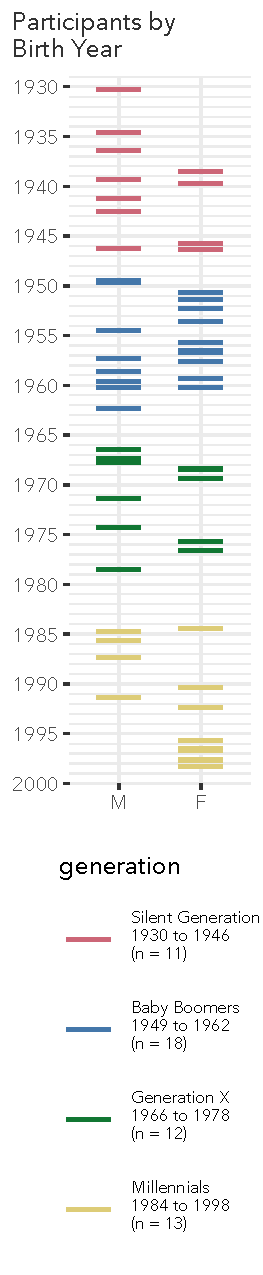
\includegraphics[width = 1.6in]{Figures/methods/age_tall.pdf}
    Figure 1.1: Age distribution by sex of the participants in this study. Some jitter has been added to view overlapping speakers.
}\addtocounter{figure}{1} % Since I manually put this figure, I'll increment the figure count.
shows the 54 speakers' birth years, divided by sex and colored by generation. There were no speakers born in 1963–1965, forming a break that happens to be around the time the Baby Boomer generation ends and Generation X begins. Furthermore, there were no speakers born 1979–1983, which was the tail end of Generation X and the beginning of the Millennials. This also corresponds to a crucial time period in Cowlitz County when the timber industry was undergoing major changes and the community was in a deep recession, as described in detail in \S\ref{sec:rise_and_fall}.

%\begin{figure*}[htb]
%    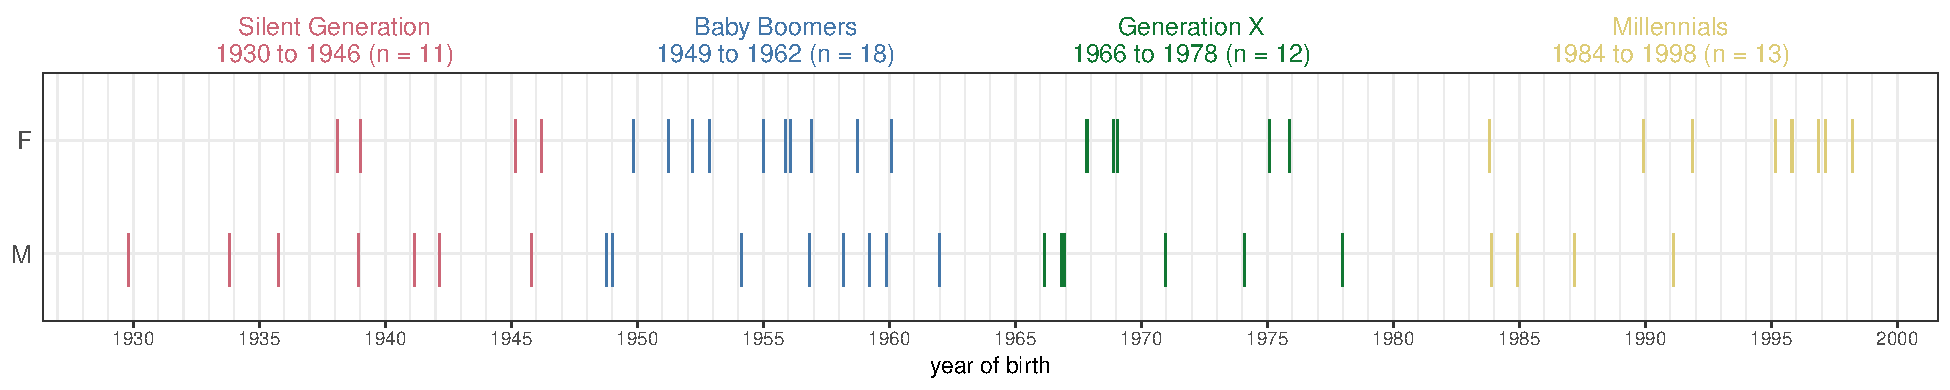
\includegraphics[width = 6.5in]{Figures/methods/age.pdf}
%    \caption[Years of birth and generations by sex.]{Years of birth and generations by sex. A small amount of jitter has been added to the birth years to allow for the viewing of multiple speakers of the same sex and the same birth year.}
%    \label{fig:age}
%\end{figure*}

There are two very small modifications to the generations defined by the Pew Research Center and the generations that will be used in the present study. First, 1946 is normally considered the first year of the Baby Boomer generation, but I felt that the two participants born in that year, Earl and Elizabeth, fit in culturally more with the Silent Generation than with the rest of the Boomers. Also, the Pew Research Center \citep{dimock_2018} has recently defined 1996 as the last year of the Millennial generation, and all those born in 1997 or later will be part of the next generation (which has not received an official name, though \textit{Generation Z} and \textit{Post-Millennial} are in circulation). In this sample, the three youngest speakers would fall into this cohort. However, it made little sense to classify those three as a separate generation, so they will be grouped with the Millennials. With these small changes in mind, these nationally recognized generational cohorts will be used as a placeholder for age in the analysis for this study.

For other demographic information, I grouped participants into broad categories. I assigned speakers binary sex based on their outward appearance. Only two participants brought up their ethnicity (one woman was half-Hispanic and another had Native American heritage); I judged all others to be Caucasian American, which is mostly what would be expected for Cowlitz County\footnote{A more complete description the demographics of Cowlitz County is provided in \S\ref{sec:physical_description}, but according to the 2017 population estimates, the county was 83.7\% White (not Hispanic or Latino) \citep{census}. In other words, I oversampled the White population with respect to the actual population.}. For the purposes of this dissertation, sexual orientation is not considered for analysis as it was rarely brought up by any of the participants, the exception being one person who self-identified as a homosexual man. Incidentally, nearly every participant who I judged to be male mentioned a wife or girlfriend and those who I judged to be female mentioned husband or boyfriend. This subjective and oversimplified classification of sex, gender, ethnicity, and sexual orientation admittedly glosses over the nuances in these features of a person's identity; future work in Cowlitz County is needed to see the effects that these factors have on language.

Each participant was assigned a pseudonym. Following \citeauthor{tagliamonte_2006} (\citeyear[51]{tagliamonte_2006}, cf. \citealt[253--254]{schlling_2013}), I refer to speakers in this dissertation by alternative names rather than numbers because they are easier to remember and give more life to their excepts. I selected names based on the person’s age and chose a name that was common during their year of birth as their pseudonym.\footnote{See Table~\ref{tab:speaker_summary} below for the list of names.}



% --------------------------------------------------------------------
% ------------------------    Processing    --------------------------
% --------------------------------------------------------------------

\section{Processing}
\label{processing}

After the interviews were completed, there are several steps of processing required to produce data in a format ready for quantitative analysis. In this section I describe the methods for transcription, forced alignment, formant extraction, and filtering, normalization, and Bark-transformation that I used in this study.

\subsection{Transcription}
\label{transcription}

The first step in data processing was to transcribe the audio. There exists software and hardware designed to facilitate transcription, but I found it easiest to simply do it manually in Praat \citep{boersma_weenink_2018_praat} for several reasons. First, after doing some preliminary tests with automatic speech-to-text software, such as the one as part of the DARLA suite \citep{reddy_stanford_2015_DARLA}, I found that it took longer to correct these transcriptions than it would have to just transcribe it myself. Second, I was most comfortable in Praat than in some other software like ELAN or Transcriber and felt like I could create more accurate boundaries to the utterance phrases than I could using other programs, given my skills in them. Finally, I wanted the output to be in Praat’s TextGrid format because I intended to use Praat scripting to extract information from the corpus, and eliminating a middle man seemed the most efficient.

I developed and adhered to some basic protocols while transcribing. I used standard English spelling with the exception of a few words like \textit{gonna}, \textit{wanna}, and \textit{cuz} (``because''). All speech was transcribed at the utterance-level regardless of syntactic boundaries. In fact, I did not attempt to parse the syntactic structure of the speech at all, so intervals were treated as continuous strings of words without regard to when prosodic phrases started or ended. Capitalization at the beginning of utterances was ignored, but it was retained in proper nouns and the pronoun \textit{I}. I likewise did not include punctuation except for apostrophes (in both contractions and possessives, which are required to distinguish words like \textit{well} and \textit{we'll}) and hyphens. All intelligible speech by the participants was transcribed, including stutters and other speech errors if an entire word was uttered. Other types of disfluencies, partially uttered words, and other noise (lip smacks, coughs, laughter) were left blank so that the forced aligner would skip over them. Interviewer speech was not transcribed; neither was speech that overlapped with the interviewers. It took 174 hours to transcribe the approximately 41 and a half hours in the conversation portion of the corpus (a rate of approximately 4.2 hours to transcribe one hour of audio).\footnote{The conversation portion of the corpus was transcribed in two waves. I did the first third April--August 2017. The remaining two-thirds were completed between April and July 2018.}

\subsection{Forced alignment}
\label{forced_alignment}

For this project, I used a local installation of the Montreal Forced Aligner \citep{macauliffe_etal_2017_MFA} to process the conversation portions of the transcribed audio. I chose this tool over other forced aligners for two reasons. First, it is relatively new and is built with Kaldi \citep{povey_etal_2011_kaldi}, which is being actively maintained and developed. Second, having the software on my own machine (as opposed to an online-based aligner like DARLA or WebMAUS) was appealing and convenient. The aligner also checks for out-of-dictionary words which facilitates the identification of typos and other misspellings, which I manually corrected. The dictionary for this aligner was the LibriSpeech corpus which will be discussed in the next section.

One of the benefits of the Montreal Forced Aligner is that it implements a speaker-level adaption in alignment. Before processing the audio, it measures acoustic properties about the speaker’s voice which it then uses to fine-tune the built-in acoustic model. However, the aligner had trouble processing the interview files because of their length, so as part of the pre-processing stage, a Praat script was written to split the audio and transcription files in half. These two halves were processed separately, though not independently. By this, I mean that the aligner was made aware that both halves came from the same speaker so the acoustic model was trained using all the speaker’s data rather than processing each half independently from the other.

Because the reading portions of the corpus were transcribed much earlier, they were processed differently. They, too, were transcribed by hand, but they were force-aligned using the DARLA suite \citep{reddy_stanford_2015_DARLA}, which, at that time, used ProsodyLab-Aligner \citep{gorman_etal_2011_prosodylab} for this task. The alignments for all segments in the word list and minimal pair tasks were hand-checked for accuracy and corrected where needed. The output of the conversation portion of the corpus was not hand-corrected, but \citet{strelluf_2019} has shown that manual correction of vowel boundaries has little effect on the results when they are presented in a summarized format, which is how they are presented in this study.

\subsection{Formant extraction}
\label{formant_extraction}

Humans use many cues from the speech signal for processing vowel sounds. Because they reflect the shape of the vocal tract, ``formants of a sound are properties of the corresponding mouth shape'' \citep[98]{ladefoged_1996}. But \citet{dipaolo_faber_1990} illustrate the need for additional acoustic variables in their analysis of what appears to be the loss of a tense-lax distinction before laterals (the \textit{feel-fill}, \textit{fail-fell}, and \textit{pool-pull} mergers) in Salt Lake City, Utah. While the vowel classes occupy the same in the F1-F2 vowel space, the laryngeal configurations of the vocal tract were used to reliably distinguish the vowel classes. Putting it succinctly, ``there is more to vowels than their formant frequencies'' \citep[201]{dipaolo_faber_1990}. Though they are not a focus of this dissertation, the multidimensional nature of speech sounds is especially true of consonants too: the distinction between what are traditionally called ``voiced'' and ``voiceless'' consonants in English can differ by as many as 16 dimensions \citep{lisker_1986}. What kind of variation is possible in these other facets of speech sounds, and what kind of social meaning can be associated with their variants?

It is out of the scope of this study to include many aspects of the speech signal in my analysis, but there is a need for other acoustic measurements in the study of the Elsewhere Shift. Because of the inconsistencies between studies that focus on these vowel changes, \citet[150]{boberg_2005} wonders whether there's more to the shift than F1 and F2. While this study will continue the trend by only using F1 and F2 measurements for analysis, I do expand my sampling of the vowel to more than just one point along its duration. \citeauthor{jacewicz_etal_2006} analyzed their data twice, once looking at midpoints alone and again looking at formants extracted at five time points, and find that ``dialect differences could well exist but remain unnoticed as a result of the less robust methodology traditionally used'' \citeyearpar[300]{jacewicz_etal_2006}. One goal for this dissertation is to show how the speech in Cowlitz County compares to other areas with the Elsewhere Shift, and the best way to maximize this comparison is to use similar methods as previous studies. For this reason, I limit my analysis to vowel formants alone, and hope that future work will describe the shift in more phonetic detail.

Once the files were transcribed and aligned, the next step in the process is to extract formant measurements from the speakers’ vowels. I chose to do this using a Praat script rather than using software such as FAVE-Extract \citep{rosenfelder_etal_2014} to allow for more flexibility in the output. In its current implementation, FAVE extracts formant measurements at five points along the duration of the vowel. While this is sufficient to analyze the trajectory of the vowel \citep{renwick_stanley_2020}, a more detailed view of these dynamic properties is possible when more data is extracted per vowel token. It is possible to modify FAVE to extract any number of tokens per vowel \citep[cf.][]{warburton_2018}, but I have found that this results in duplicate measurements across multiple time points, which is an undesirable result.

The script that I used for formant extraction was one that I wrote in Praat. Similar to the Montreal Forced Aligner, the software had difficulty processing the entire interviews at once, so the script first split the file into more manageable chunks that were approximately five-minutes long, ensuring that the split did not interrupt the informants' speech. For each vowel, measurements were taken at 11 equidistant points along its duration (onset, 10\%, 20\%, \ldots, 90\%, offset). I processed the audio four times, each using a different combination of settings in Praat. I altered the number of formants Praat should look for and the maximum Hz to consider when looking for those formants. The four combinations of settings were 5 formants with a maximum of 4500Hz, 5000Hz, and 5500Hz and 6 formants with a maximum of 5500Hz. This resulted in four versions of the data for each speaker, each produced slightly different settings and resulting in slightly different formant measurements.

The reason for this apparent redundancy was because a single combination of settings usually does not produce the cleanest results from the entire audio corpus. I had men and women in this sample with relatively high and low voices, so even different settings based on the sex of the speaker was not adequate. FAVE handles this issue by extracting four sets of measurements per token and selects the best based on distances from hand-checked measurements \citep[34--36]{labov_etal_2013}. My initial goal was to extract data using many more settings and use what I call the ``mistplot'' technique (\citealt{stanley_2018_mistplots}; see also \citealt{kendall_vaughn_2015}) to determine the best measurements, but constraints on time and computational power prohibited me from using this method in this project. Instead, to determine the best measurements, I simply plotted all data in the F1-F2 space and selected the set that appeared the cleanest per speaker, meaning I chose the setting that produced the fewest obvious gross outliers. For women, the most common setting was using five formants and 5000Hz, with the exception of six women (they all had relatively higher voices) whose best setting was 6000Hz. For the men, the most common setting was five formants and 5000Hz except for the three men whose voices were relatively higher voices and 5500Hz yielded cleaner results. There is admittedly some subjectivity in this selection technique, but I feel that the results were cleaner than applying the same settings for all speakers of the same sex.

\subsection{Filtering}
\label{filtering}

It is out of the scope of this dissertation to analyze all tokens of all vowels. I filtered out vowels that did not have primary lexical stress. I also removed diphthongs (\price, \mouth, and \choice) and syllabic /\textipa{\textrhookschwa}/ (\nurse). Finally, I excluded words if they were part of a 181-item list of stop words (see Appendix~\ref{appendix:stopwords}). Here, stop words were defined as words that are high frequency (including discourse markers like \textit{yeah} and \textit{y'know}), many of which were members of a closed class lexical category in English like pronouns and conjunctions.

Automatic methods in forced alignment and formant extraction save time, make it easier to process larger corpora, and are more objective than manual work; however, they come at the expense of data cleanliness. Manual checking and correcting of outliers was not done in this study, largely due to the size of the corpus. Tens of thousands of vowel tokens, each contributing 22 formant measurements (two formants at 11 time points), was judged to be too large to check by hand. As such, a method for filtering the data was necessary to exclude out the inevitable outliers in the data that are present because of software errors.

One of the most common methods for automatic detection and exclusion of outliers is to remove observations that have F1 or F2 measurements more than two standard deviations from the mean (a \textit{z}-score method). I argue that this method is inherently flawed because of the unnaturally rectangular distribution it produces. F1 and F2 represent height and backness axes, respectively, but tokens of the same vowel phoneme often fall along distributions that are diagonal to these dimensions. When F1 and F2 are correlated like this, bad tokens may fall within the normal range of formant values but they are still considered good data. Meanwhile, good data on the extremities of the distribution may be excluded.

Another method for detecting outliers is to calculate the Mahalanobis distance from each token to that vowel’s mean in a multivariate space \citep{mahalanobis_1936, renwick_ladd_2016, labov_etal_2013, evanini_2009_diss}. This method considers the distribution and correlation between the F1 and F2 measurements such that observations that a human would spot as outliers are often detected as such. Visually, this can be thought of as fitting an ellipse of some size to the data, centered around the mean, and anything outside of that ellipse is considered an outlier.

\begin{figure*}[tb]
    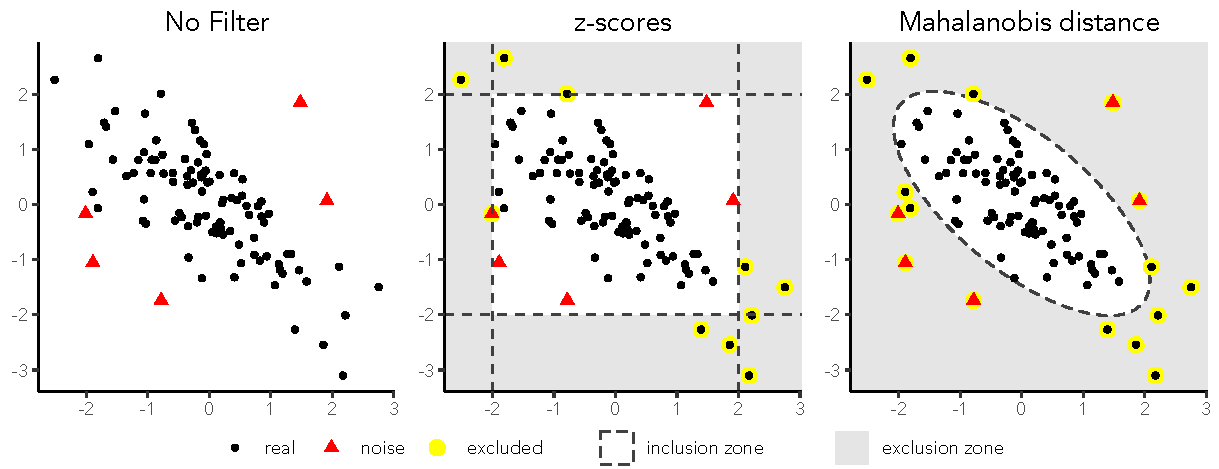
\includegraphics[width = 6.5in]{Figures/methods/filtering.pdf}
    \caption[A comparison of filtering methods]{A comparison of filtering methods on simulated data.}
    \label{fig:filtering}
\end{figure*}

Figure~\ref{fig:filtering} compares these two methods. For this plot, I generated 100 points based on a multivariate normal distribution and then added five points known to be outliers. The generated observations are plotted as black circles and the outliers as red triangles. This data is seen in the left panel of Figure~\ref{fig:filtering} and it is evident that though the outliers have F1 and F2 measurements that fit in with the rest of the data, it is the combination of their measurements (i.e. high F1 and F2 or low F1 and F2) that place them in areas relatively far from other data points. In the center panel, I apply a filter that excludes tokens if their F1 or F2 measurements are further than two standard deviations from the mean. These cutoff values are represented by the dashed lines and observations that fall outside of the square are highlighted in yellow. This center panel shows that none of the known outliers were excluded, but eight of the good points were. Another way of think about this technique is that it essentially fits a square cookie cutter to an ellipsoidal distribution. On the contrary, the right panel in Figure~\ref{fig:filtering} illustrates the filter based on the Mahalanobis distance. The dotted line in this panel encircles the area where the square root of the Mahalanobis distance is less than two, roughly corresponding to two standard deviations from the mean. Since this simulated data is ellipsoidal, the oval-shaped “cookie cutter” does a better job, and it excludes all of the known outliers. However, it is still not a perfect method because eight good data points were also excluded (mostly matching the eight removed in the center panel).

For this study, I chose to use the Mahalanobis distance as a way to detect potential outliers. For each vowel for each speaker, after the measurements from all time points were pooled together and were arranged by their multidimensional distance (in the F1-F2 space) from the mean, I did a blanket exclusion of the furthest 5\% of the tokens, which roughly corresponds to removing observations if the square root of their Mahalanobis distance is greater than two.

The use of the Mahalanobis distance is not without its flaws. Statistically, this method is sensitive to outliers because it relies on vowel means. The presence of many gross outliers can skew the distribution, causing the mean to be pulled to an unexpected position in the vowel space. When the mean is far enough from the ``true'' center of the distribution, good measurements may fall far enough from it that they get removed by the filter.\footnote{In \citet{stanley_2018_mistplots} I presented a preliminary modified version of the Mahalanobis distance for outlier detection that is less sensitive to outliers. For more information, see the \texttt{joeyr} package \citep{joey_2020_joeyr}. Due to limitations of computational power and time constraints, this technique was not implemented in this study. } The other flaw in the Mahalanobis filter is that it assumes that vowel data is multivariate normally distributed. \citet{vanhofwegen_2017_diss} has shown that this is not the case because speakers can make use of stylistic variants that cluster at the extremes of the distribution of the vowel tokens in other situations. To my knowledge, there is no best method for detecting and excluding potential outliers in sociophonetic data, but using the Mahalanobis distance method seems more theoretically-grounded and more appropriate---or at least less bad---than using standard deviations of F1 and F2 measurements.


\subsection{Normalization}
\label{normalization}

Because of physiological differences in humans, there is considerable variation in the formant measurements between speakers. Women and people with shorter vocal tracts tend to have higher formants and a larger overall vowel space while men and people with longer vocal tracts have lower formants. For computational processing, these differences are problematic when two people pronounce a vowel, because though a human would perceive the two to be the ``same,'' the formant values between two pronunciations may be quite different. For this reason, some sort of normalization procedure is desirable to allow for meaningful comparisons between speakers.

There is a myriad of normalization procedures in circulation today. A detailed account of how they are calculated and how well they appear to work is out of the scope of this dissertation, though \citet{adank_etal_2004} and the methods page of the \textit{NORM} suite \citep{thomas_kendall_2007_NORM} are good resources for this information. Recently, \citet{barreda_2019} has shown that the \citet{lobanov_1971} transformation is inherently flawed because it operates on F1 and F2 independently, is too powerful, and aims at a goal that is theoretically unsound. Instead, he advocates for some sort of log-mean-based method which applies a single metric to both F1 and F2 and is empirically well-supported. He does not claim that a log-based method is ``correct,'' but rather that it is less bad than the Lobanov transformation.

In this study, I use the log-mean normalization method adopted by the \textit{Atlas of North American English}. Their method, which is based on the one established by \citet{nearey_1978_diss}\footnote{See \citet[519 note 2]{barreda_nearey_2018} for a details on how this method differs from the original \citet{nearey_1978_diss} method.} was found to be ``most effective in eliminating the male-female differences due to vocal tract length and preserving the social stratification of stigmatized variables that had been established by auditory impressions'' \citep{labov_ash_boberg_2006_anae}. Rather than using the geometric mean (G) for the Telsur project (6.896874), I calculated the mean based on the Cowlitz County speakers (6.801067). Note that the Telsur G is based on single-point measurements per vowel; it is unclear how this method should be applied to trajectory data. It made little intuitive sense to normalize each time point individually, so my sample's geometric mean was calculated based on measurements from all time points pooled together.\footnote{For reference, the geometric mean for this sample based on midpoints alone was 6.813876.} These calculations were made using a custom script in R.


\subsection{Bark-transformation}
\label{sec:barks}

In this study, I applied a double transformation to the data. After the data was normalized, it was then converted into Barks. Barks are a unit of measurement that is ``based upon the natural division of the audible frequency range by the ear'' \citet[248]{zwicker_1961}. However, because Zwicker's original proposal only provided Hz-equivalent values for integer values of Barks (\textit{i.e.} 6 Barks = 570 Hz, 7 Barks = 700 Hz, 8 Barks = 840 Hz, etc.), various equations have since been developed to convert any Hz measurements into Barks. The formula that \citet{traunmuller_1990} determined was best, after comparison with several other proposed formulas, was the one used in this study.\footnote{For Bark values less than 2 or greater than 20.1, corresponding to approximately 200 Hz and 6500 Hz, respectively, a slightly different formula is used to make the relationship more linear. On the upper end, this was not an issue because measurements did not exceed 16 Barks. On the lower end, just 6 measurements did fall below 2 Barks, and applying the transformation did not result in a change of more than 0.07 Barks.} That is, if $f$ is a formant measurment, than its Bark equivalent is calculated as \(26.81 \times \frac{f}{1960+f} - 0.53\).

There are several reasons for using the Bark scale. First, formant frequencies do not follow a normal distribution, primarily because they are logarithmic. A difference in 100 Hz in the F1 range is perceptually larger than in the F2 range. Similarly, a difference in 100 Hz for back vowels’ F2 is perceptually larger than for front vowels. The Bark transformation converts frequencies into a linear scale to approximate human perception such that the difference between 5 and 6 Barks is perceptually similar to the difference between 15 and 16 Barks.

The second reason for applying Barks to the normalized data is because regression models---like the kind used in this study---assume a normal distribution in their residuals. That is, the differences between predicted values and observed values in a regression model should be normally distributed with no obvious patterns. When linear models are fit to formant frequencies, the variance of the residuals is correlated with the predicted values.\footnote{Statisticians call this \textit{hetero\-scedasticity}.} This correlation indicates that there is some pattern that has not been captured by the model. Transforming logarithmic data to a linear scale helps remedy this problem. In general, transformations are a legitimate technique in regression modeling and are commonly used by statisticians when working with logarithmic data \citep{gelman_hill_2007}. The Bark scale is an appropriate transformation for this kind of data, and a model fit to Barks instead of Hz is likely to have more normally distributed residuals and have a more reliable output.

Finally, because of how the particular models were implemented (see \S\ref{gamms_in_this_study}), converting the dependent variable to Barks resulted in more appropriately-sized confidence intervals for each formant. F1 and F2 were pooled together to create a single response variable, and though the model was told which formant each measurement came from, the model could not account for the fact that the variances between the two sets of formant measurements were different. When selecting the appropriate model for this study, I noticed that the confidence intervals for F1 values were large, so somewhat drastic differences between groups were not considered to be statistically significant. Meanwhile, the F2 confidence intervals were smaller, and even small shifts in the vowel space were considered statistically significant. Overall, these earlier models suggest far more movement along the front-back dimension rather than in vowel height.\footnote{As pointed out in \S\ref{sec:structure_of_elsewhere_shift}, determining whether vowels are lowering or retracting is crucial in the study of the Elsewhere Shift. Lowering suggests a chain shift and retraction suggests parallel movement. Given that some researchers have found one and not the other (or perhaps one and then the other) suggests that different communities do different things. I wanted to make sure that my methods did not inherently bias the results into suggesting one or the other.} The reason for this was because of the pooled formant values. The model produced similar confidence intervals for both formants, which ended up being too large for F1 and too small for F2. To correct this error, I transformed the already-normalized data into the Bark scale. This way, the model still produces similar confidence intervals for F1 and F2, but this is appropriate given the nature of the Bark scale.

Some readers may be concerned that a double transformation---that is, Bark-transformation on data that has already been normalized---abstracts too far from reality.\footnote{While much of this dissertation shows that traditional methods are not always ideal, a double data transformation has been used to study vowel data in the West. \citet[49]{hall_lew_2009_diss} converts Hz to Bark and then applies the Lobanov transformation, \citet[166]{podesva_etal_2015} converts tokens into Barks and then normalized using the modified Watt and Fabricius \textit{S}-centroid method, and \cite[198]{donofrio_etal_2019} converts to Barks first and then applies the Nearey \citeyearpar{nearey_1978_diss} method. Nevertheless, the techniques in this paper differ in that they normalized the data first and \textit{then} apply the Bark transformation.} I agree that the best model would be fit to the raw formant values, but I have not yet been satisfied with a statistical model that does so.\footnote{\citet{drager_hay_2012} illustrate including speaker as a random intecept in a linear mixed-effects model can serve as a way to normalize the data, but it is out of the scope of this study to determine whether this process also applies in a GAMM.} When measured in Hz, people with higher voices will have a larger vowel space (and consequently, a larger variance in formant values) than those with lower voices. Adding speaker as a random intercept can help correct differences in the position of speakers’ formants, but not necessarily the \textit{spread} of the formants. A log-based normalization procedure such as the \textit{ANAE} method used in this study can, and a transformation from logarithmic to linear is one way to bring the numbers closer to how humans perceive sound.




% --------------------------------------------------------------------
% -----------------------    Word Classes    -------------------------
% --------------------------------------------------------------------

\section{Word classes}
\label{word_classes}

English vowels are influenced significantly by the consonants that surround them \citep{olive_etal_1993}. Much of this is simply allophonic and the patterns found in this sample are no different than what phoneticians have been describing for decades. However, in this sample, there are patterns in some vowel classes that cannot be ascribed to phonological factors alone, so sociolinguistic explanations are needed to account for this variation. Because the focus of this discussion is on these allophones, it is requisite to state how they are defined and what their labels are.

Many of the ongoing changes in the West affect specific allophones of \trap, \dress, and \kit. For example, the \textit{Atlas of North American English} \citep[169--184]{labov_ash_boberg_2006_anae} illustrates vowel patterns of individuals with various configurations of \trap. One speaker from New York City exhibits the split-/\textipa{\ae}/ system, a complex pattern of raising in certain lexical and phonological environments. But most notably, this speaker has a raised \trap before coda nasals (\textit{pants}, \textit{lamb}), but a lax variant before intervocalic nasals (\textit{family}, \textit{Spanish}), velar nasals (\textit{language}), and /\textipa{g}/ (\textit{tag}, \textit{bag}). Another speaker from Columbus, Ohio has a higher vowel before all nasals (\textit{pants}, \textit{family}, \textit{banking}) and a lower vowel elsewhere, including pre-/\textipa{g}/. Finally, a third speaker from Edmonton, Alberta has no clear division between raised and unraised variants, but in the continuum, prenasal and pre-/\textipa{g}/ tokens were among the highest. In other words, nearly all speakers in their sample had raised \trap before /\textipa{m}/ and /\textipa{n}/, but whether pre-/\textipa{N}/ tokens or pre-/\textipa{g}/ were raised depended on the variety of English.

For this reason, it is prudent to divide \trap into at least four allophones: pre-/\textipa{m},\textipa{n}/, pre-/\textipa{N}/, pre-/\textipa{g}/, and elsewhere. By analogy, \dress and \kit are also split into four allophones based on the same contextual environments, following \citet{cardoso_etal_2016_pads}. Some of these allophones have not been anaylzed in great detail in the West, so it is unclear whether, for example, all prenasal allophones form a natural class and exhibit the same behavior.\footnote{In fact, in Chapter~\ref{ch:prenasal}, I show that they in fact do not pattern together in this corpus, though this finding was only possible by splitting the data this way and testing the hypothesis of natural classes across prenasal allophones of the lax vowels.} Though \citet{moonwomon_1991_diss} and \citet{swan_2016_proceedings} differentiate pre-stop and pre-fricative allophones, and \citep{labov_ash_boberg_2006_anae} analyze pre-voiced and pre-voiceless stops separately, I choose not to follow these divisions since the variation found here was largely predictable and did not appear to vary by social factors.

% This is out of place but it's only to get it positioned correctly on the page.
\begin{table*}[p!]
    \caption{Summary of basic demographics and tasks completed by each speaker.}
    \centering
    \resizebox{0.85\textwidth}{!}{
        \begin{tabular}{ l | c c c | c c c c c |}
 & \multicolumn{3}{|c|}{\textbf{Demographics}} & \multicolumn{5}{|c|}{\textbf{Tasks}} \\
Pseudonym & Sex & Age & Gen. & Convo. & Friends & Cat Mice & Word List & Min. Pairs \\
\hline
Billy     & M & 86 & \multirow{11}{1.25em}{\rotatebox{90}{Silent Generation}}
                    & \ding{51} &           &           &           &  \\
Keith     & M & 82 && \ding{51} &           &           &           &  \\
Dale      & M & 80 && \ding{51} & \ding{51} &           &           &  \\
Betty     & F & 78 && \ding{51} &           &           &           &  \\
Helen     & F & 77 && \ding{51} & \ding{51} &           &           & \ding{51} \\
Arthur    & M & 77 && \ding{51} &           &           &           &  \\
Curtis    & M & 75 && \ding{51} & \ding{51} &           &           &  \\
Rob       & M & 74 && \ding{51} & \ding{51} & \ding{51} & \ding{51} & \ding{51} \\
Margaret  & F & 71 && \ding{51} & \ding{51} & \ding{51} &           & \ding{51} \\
Elizabeth & F & 70 && \ding{51} & \ding{51} &           &           & \ding{51} \\
Earl      & M & 70 && \ding{51} & \ding{51} &           &           & \ding{51} \\
\hdashline
Ed        & M & 67 & \multirow{18}{1.25em}{\rotatebox{90}{Baby Boomers}}
                    & \ding{51} & \ding{51} &           &           &  \\
Harold    & M & 67 && \ding{51} &           &           &           &  \\
Marilyn   & F & 66 && \ding{51} & \ding{51} &           & \ding{51} & \ding{51} \\
Martha    & F & 65 && \ding{51} & \ding{51} & \ding{51} & \ding{51} & \ding{51} \\
Kay       & F & 64 && \ding{51} & \ding{51} & \ding{51} & \ding{51} & \ding{51} \\
Patricia  & F & 63 && \ding{51} & \ding{51} & \ding{51} & \ding{51} & \ding{51} \\
Anthony   & M & 62 && \ding{51} &           &           &           &  \\
Kathleen  & F & 61 && \ding{51} & \ding{51} & \ding{51} & \ding{51} & \ding{51} \\
Laura     & F & 60 && \ding{51} & \ding{51} & \ding{51} & \ding{51} & \ding{51} \\
Teressa   & F & 60 && \ding{51} & \ding{51} & \ding{51} & \ding{51} & \ding{51} \\
Kathryn   & F & 59 && \ding{51} &           & \ding{51} & \ding{51} &  \\
Rich      & M & 59 && \ding{51} & \ding{51} & \ding{51} & \ding{51} & \ding{51} \\
Bruce     & M & 58 && \ding{51} &           &           &           &  \\
Carol     & F & 57 && \ding{51} & \ding{51} &           & \ding{51} & \ding{51} \\
Doug      & M & 57 && \ding{51} & \ding{51} & \ding{51} & \ding{51} & \ding{51} \\
Robin     & F & 56 && \ding{51} & \ding{51} & \ding{51} & \ding{51} & \ding{51} \\
Darrell   & M & 56 && \ding{51} & \ding{51} & \ding{51} & \ding{51} & \ding{51} \\
Craig     & M & 54 && \ding{51} & \ding{51} & \ding{51} & \ding{51} & \ding{51} \\
\hdashline
Ron       & M & 50 & \multirow{11}{1.25em}{\rotatebox{90}{Generation X}}
                    & \ding{51} & \ding{51} & \ding{51} & \ding{51} & \ding{51} \\
Daniel    & M & 49 && \ding{51} & \ding{51} & \ding{51} & \ding{51} & \ding{51} \\
Kevin     & M & 49 && \ding{51} & \ding{51} &           &           & \ding{51} \\
Kim       & F & 48 && \ding{51} & \ding{51} & \ding{51} & \ding{51} & \ding{51} \\
Donna     & F & 48 && \ding{51} & \ding{51} & \ding{51} & \ding{51} & \ding{51} \\
Cynthia   & F & 47 && \ding{51} & \ding{51} & \ding{51} & \ding{51} & \ding{51} \\
Cindy     & F & 47 && \ding{51} &           &           &           & \ding{51} \\
Shane     & M & 45 && \ding{51} & \ding{51} & \ding{51} &           & \ding{51} \\
Jason     & M & 42 && \ding{51} & \ding{51} &           &           & \ding{51} \\
Carla     & F & 41 && \ding{51} & \ding{51} & \ding{51} & \ding{51} & \ding{51} \\
Holly     & F & 40 && \ding{51} & \ding{51} & \ding{51} & \ding{51} & \ding{51} \\
Ryan      & M & 38 && \ding{51} & \ding{51} & \ding{51} &           & \ding{51} \\
\hdashline
Crystal   & F & 32 & \multirow{13}{1.25em}{\rotatebox{90}{Millennials}}
                    & \ding{51} & \ding{51} & \ding{51} & \ding{51} & \ding{51} \\
Andrew    & M & 32 && \ding{51} & \ding{51} & \ding{51} & \ding{51} & \ding{51} \\
Sean      & M & 31 && \ding{51} & \ding{51} & \ding{51} & \ding{51} & \ding{51} \\
Scott     & M & 29 && \ding{51} & \ding{51} & \ding{51} & \ding{51} & \ding{51} \\
Amanda    & F & 26 && \ding{51} & \ding{51} & \ding{51} & \ding{51} & \ding{51} \\
Brandon   & M & 25 && \ding{51} & \ding{51} & \ding{51} & \ding{51} & \ding{51} \\
Megan     & F & 24 && \ding{51} & \ding{51} & \ding{51} & \ding{51} & \ding{51} \\
Amber     & F & 21 && \ding{51} & \ding{51} & \ding{51} & \ding{51} & \ding{51} \\
Alyssa    & F & 20 && \ding{51} & \ding{51} &           & \ding{51} & \ding{51} \\
April     & F & 20 && \ding{51} & \ding{51} & \ding{51} & \ding{51} & \ding{51} \\
Kayla     & F & 19 && \ding{51} & \ding{51} & \ding{51} & \ding{51} & \ding{51} \\
Hannah    & F & 19 && \ding{51} & \ding{51} &           &           & \ding{51} \\
Jessica   & F & 18 && \ding{51} &           &           &           & \ding{51}
        \end{tabular}
    }
    \label{tab:speaker_summary}
\end{table*}


One potential category that was ultimately discarded was \bash (\trap before /\textipa{S}/). While transcribing my data, I heard several of the older speakers use a raised offglide in this environment (\textit{ash} [\textipa{\ae \textsubarch{I}S}]). This is attested in Indiana \citep{carmony_1970}, California \citep{galloway_1967}, and eastern areas of the South and parts of New England (\citealt[104]{kurath_mcdavid_1961}; see also \citealt[41--42, footnote 27]{labov_1991}), but no study that I am aware of has treated this vowel class distinctly from other allophones of \trap. Unfortunately, I likewise cannot give proper attention to this vowel class because it is out of the scope of this dissertation. Therefore, tokens of \bash will be grouped together with \bat.



% --------------------------------------------------------------------
% -----------------------    Corpus Size    --------------------------
% --------------------------------------------------------------------

\section{Corpus size and constitution}
\label{corpus_size_constitution}

I interviewed 54 participants in the approximately five weeks I spent in Cowlitz County. Table~\ref{tab:speaker_summary} shows the sexes, ages, and generations of all 54 speakers as well as which tasks they completed. As was stated previously, while I was able to interview everyone, not all participants completed all tasks due to limited time, vision, or reading ability (particularly in the Silent generation). Other demographic information such as ethnicity, sexual orientation, religion, and what city within the county they grew up in are not considered in this dissertation and are not shown in Table~\ref{tab:speaker_summary}. Other information that is less quantifiable and not as easily summarized in a table, such as their connection and strength of their connection to the Mills or their feelings about the Pacific Northwest and specific cities within the region, are also not provided in this table, though that information will be used as needed in this study.

\begin{table*}[tb!]
    %\captionsetup{style=joey-wide-center}
    \caption{Number of tokens for each part of the corpus.}
    \centering
    \liningnums{
        \begin{tabular}{l c r r r r r}
    Task                                & Participants & \multicolumn{2}{c}{Time} & Words & Total Vowels & Vowels Analyzed \\
    \hline
    \textbf{Conversation}               & \textbf{54}  & \textbf{41h} & \textbf{26m} & \textbf{325,541} & \textbf{404,959} & \textbf{116,104} \\
    \textbf{Reading}                    & \textbf{47}  & \textbf{3h} & \textbf{50m} & \textbf{21,955} & \textbf{27,636} & \textbf{12,266} \\
    \hspace{1em}``Friends''              & 44 &  & 14m & 2,479 & 2,916 & 920 \\
    \hspace{1em}``The Cat and the Mice'' & 33 & 1h & 7m & 12,771 & 14,972 & 4,591 \\
    \hspace{1em}Word List              & 33 & 1h & 12m & 5,190 & 7,679 & 4,926 \\
    \hspace{1em}Minimal Pairs          & 43 & 1h & 27m & 1,515 & 2,069 & 1,829 \\
    \cline{2-7}
                                   & Total: & 45h & 16m & 347,496 & 432,595 & 128,370
        \end{tabular}
    }
    \label{tab:corpus_constitution_table}
\end{table*}


As seen in Table~\ref{tab:corpus_constitution_table}, these interviews contained a total of 45 hours 16 minutes of audio and 347,496 words. From these words, measurements from 432,595 vowels were extracted, but after passing these through the filters described above,\footnote{Recall that the majority of this corpus of natural speech consists of stop words or vowels without lexical stress, explaining why over two-thirds of the total number of vowel tokens were lost. Filtering from Mahalanobis distances removed relatively few tokens in comparison.} 128,370 vowels remained for this study. Table~\ref{tab:corpus_constitution_table} also shows how this data was divided among the tasks.

For the bulk of this study, the reading style was actually excluded from analysis. At the time of data collection, my principal objective was not to describe the Elsewhere shift, so the prepared materials did not specifically elicit many tokens of these vowels (particularly the prenasal and pre-/\textipa{N}/ environments) so there was not enough for a robust analysis of style. In two cases do I discuss some findings from these tasks (\S\ref{BENG} and \S\ref{ch:low_back}), but for the main analysis, only the conversation portion of the corpus is used.

\newgeometry{margin=1in}
\begin{landscape}
\begin{table}[p!]
    \caption{Summary of word classes in this study.}
%\begin{sidewaystable}[p!]
    \centering
    \resizebox{9in}{!}{%
        \begin{tabular}{c  |  l r p{6cm}  |  l r p{6cm}  |  l r p{6cm} }
             \multirow{2}{*}{\shortstack{\textbf{Following}\\\textbf{Consonant}}} &
             \multicolumn{3}{c|}{\textbf{\Large\trap}} &
             \multicolumn{3}{c|}{\textbf{\Large\dress}} &
             \multicolumn{3}{c}{\textbf{\Large\kit}} \\

             &
             Label & n & 20 most frequent words &
             Label & n & 20 most frequent words &
             Label & n & 20 most frequent words \\
             \hline
             /\textipa{m} or \textipa{n}/ &
                \ban &
                    \liningnums{2,461} &
                    \textit{family}, \textit{man}, \textit{can}, \textit{plan}, \textit{grandma}, \textit{stand}, \textit{understand}, \textit{camp}, \textit{hand}, \textit{ran}, \textit{grandpa}, \textit{began}, \textit{band}, \textit{aunt}, \textit{animals}, \textit{Montana}, \textit{grand}, \textit{handle}, \textit{grandparents}, \textit{January} &
                \ben &
                    \liningnums{4,823} &
                    \textit{went}, \textit{remember}, \textit{anyway}, \textit{anything}, \textit{ten}, \textit{friend}, \textit{many}, \textit{end}, \textit{twenty}, \textit{anywhere}, \textit{anybody}, \textit{center}, \textit{sent}, \textit{Henry}, \textit{pen}, \textit{spend}, \textit{elementary}, \textit{pretend}, \textit{den}, \textit{Wednesday} &
                \bin &
                    \liningnums{1,936} &
                    \textit{since}, \textit{interesting}, \textit{simply}, \textit{minutes}, \textit{timber}, \textit{pin}, \textit{din}, \textit{innocent}, \textit{dinner}, \textit{industry}, \textit{finish}, \textit{cinnamon}, \textit{swimming}, \textit{within}, \textit{inch}, \textit{window}, \textit{swim}, \textit{interest}, \textit{beginning}, \textit{similar} \\
    & & & & & & & \\
            /\textipa{N}/ &
                \bang &
                    \liningnums{265} &
                    \textit{hang}, \textit{language}, \textit{angry}, \textit{thank}, \textit{tank}, \textit{bank}, \textit{ankle}, \textit{Frankfurt}, \textit{slang}, \textit{Anchorage}, \textit{hanger}, \textit{Shanghai}, \textit{Da Nang}, \textit{angle}, \textit{dang}, \textit{hangout}, \textit{sank}, \textit{anchor}, \textit{bang}, \textit{blank} &
                \beng &
                    \liningnums{74} &
                    \textit{length}, \textit{strength}, \textit{lengths}, \textit{strengthen} &
                \bing &
                    \liningnums{2,226} &
                    \textit{think}, \textit{thing}, \textit{bring}, \textit{king}, \textit{single}, \textit{English}, \textit{drink}, \textit{spring}, \textit{sing}, \textit{ring}, \textit{England}, \textit{swing}, \textit{finger}, \textit{pink}, \textit{ink}, \textit{Kingsberry}, \textit{Lincoln}, \textit{sink}, \textit{ting}, \textit{bingo} \\
    & & & & & & & \\
          /\textipa{g}/ &
                \bag &
                    \liningnums{138} &
                    \textit{bag}, \textit{wagon}, \textit{jaguar}, \textit{nagging}, \textit{rag}, \textit{agony}, \textit{brag}, \textit{dragon}, \textit{zigzagged}, \textit{snag}, \textit{tag}, \textit{drag}, \textit{flag}, \textit{Yakataga}, \textit{baggie}, \textit{Flagstaff}, \textit{magazine}, \textit{baggage}, \textit{lag}, \textit{Niagara} &
                \beg &
                    \liningnums{391} &
                    \textit{leg}, \textit{peg}, \textit{beg}, \textit{integrity}, \textit{legacy}, \textit{egg}, \textit{oregano}, \textit{pregnant}, \textit{regular}, \textit{preggo}, \textit{negative}, \textit{Greg}, \textit{Peggy}, \textit{segment}, \textit{segregated} &
                \jbig &
                    \liningnums{837} &
                    \textit{big}, \textit{figure}, \textit{pig}, \textit{zigzagged}, \textit{dig}, \textit{Ligeti}, \textit{rig}, \textit{signal}, \textit{signet}, \textit{trigger}, \textit{biggie}, \textit{Brigham}, \textit{gig}, \textit{giggle}, \textit{ignorant}, \textit{indignant}, \textit{jigsaw}, \textit{Rigby}, \textit{signalman}, \textit{signature} \\
    %        /\textipa{S}/ &
    %            \bash &
    %                229 &
    %                \textit{ash}, \textit{(inter)national}, \textit{cash}, \textit{flash}, \textit{crash}, \textit{Nash}, \textit{passion}, \textit{fashion}, \textit{mashed}, \textit{hash (browns)}, \textit{trash}, \textit{old-fashioned}, \textit{splash}, \textit{ashen}, \textit{Ashley}, \textit{bashful}, \textit{compassion}, \textit{dash}, \textit{ration}, \textit{succotash} &
    %            \multicolumn{3}{c}{NA} &
    %            \multicolumn{3}{c}{NA} \\
    %        /\textipa{\*r}/ &
    %            \marry &
    %                32 &
    %                &
    %            \merry &
    %                2,012 &
    %                \textit{Weyerhaeuser}, \textit{heritage}, \textit{sheriff}, \textit{terrible}, \textit{numeric}, \textit{American}, \textit{berry}, \textit{Eric} &
    %            \mirror &
    %                1,319 &
    %                \textit{year}, \textit{weird}, \textit{near}, \textit{experience}, \textit{clear}, \textit{Rainier}, \textit{career}, \textit{beer}, \textit{period}, \textit{spirit}, \textit{engineer}, \textit{deer}, \textit{gear}, \textit{theory}, \textit{serious}, \textit{material}, \textit{cheers}, \textit{Sears}, \textit{Syracuse}, \textit{ear} \\
    %        /\textipa{l}/ &
    %            \pal &
    %                262 &
    %                \textit{valley}, \textit{gal}, \textit{Italian}, \textit{gallon}, \textit{alcohol}, \textit{Alex}, \textit{Alan}, \textit{challenge}, \textit{Dallas}, \textit{Fallon}, \textit{mentality}, \textit{Valentine's}, \textit{alphabet}, \textit{balance}, \textit{reality}, \textit{valve}, \textit{album}, \textit{Alice}, \textit{allergies}, \textit{caliber} &
    %            \fell &
    %                2842 &
    %                \textit{well}, \textit{Kelso}, \textit{tell}, \textit{else}, \textit{help}, \textit{twelve}, \textit{Helens}, \textit{L}, \textit{felt}, \textit{fell}, \textit{sell}, \textit{hotel}, \textit{welding}, \textit{health}, \textit{elders}, \textit{helicopter}, \textit{welcome}, \textit{developed}, \textit{smell}, \textit{held} &
    %            \jfill &
    %                2,606 &
    %                \textit{really}, \textit{still}, \textit{building}, \textit{built}, \textit{hill}, \textit{children}, \textit{will}, \textit{mill}, \textit{build}, \textit{milk}, \textit{Billy}, \textit{thrill}, \textit{kill}, \textit{military}, \textit{skills}, \textit{film}, \textit{till}, \textit{fill}, \textit{silver}, Bill \\
    & & & & & & & \\
            elsewhere &
                \bat &
                    \liningnums{5,403} &
                    \textit{back}, \textit{actually}, \textit{cat}, \textit{dad}, \textit{last}, \textit{bad}, \textit{Castle (Rock)}, \textit{class}, \textit{half}, \textit{happened}, \textit{passed}, \textit{Seattle}, \textit{ask}, \textit{catch}, \textit{fact}, \textit{happy}, \textit{black}, \textit{graduated}, \textit{exactly}, \textit{Saturday} &
                \bet &
                    \liningnums{8,478} &
                    \textit{said}, \textit{yes}, \textit{never}, \textit{everything}, \textit{every}, \textit{ever}, \textit{get}, \textit{next}, \textit{everybody}, \textit{whatever}, \textit{together}, \textit{guess}, \textit{yep}, \textit{says}, \textit{let}, \textit{seven}, \textit{second}, \textit{left}, \textit{met}, \textit{better} &
                \bit &
                    \liningnums{9,322} &
                    \textit{different}, \textit{little}, \textit{kid}, \textit{pretty}, \textit{live}, \textit{six}, \textit{bit}, \textit{river}, \textit{Christmas}, \textit{give}, \textit{sister}, \textit{city}, \textit{middle}, \textit{business}, \textit{mission}, \textit{fifty}, \textit{picture}, \textit{pick}, \textit{bridge} \\
    & & & & & & & \\
            \cline{2-3}\cline{5-6}\cline{8-9}
            &
            \multicolumn{2}{c}{Total: \liningnums{10,102}} &
            &
            \multicolumn{2}{c}{Total: \liningnums{18,546}} &
            &
            \multicolumn{2}{c}{Total: \liningnums{18,246}} &
            \\
        \end{tabular}
    }
    \label{tab:word_classes}
%\end{sidewaystable}
\end{table}
\end{landscape}
\loadgeometry{sidenote}


Table~\ref{tab:word_classes} provides an overview of the allophones considered in this dissertation. For each major column, the phonemes \trap, \dress, and \kit are listed. Each row represents different phonological environments. Within each cell of the table, I provide the Wells-inspired label in small caps, the number of tokens in that category, and up to 20 of the most frequent words for that allophone within this corpus. Some of these allophones contain relatively few tokens; for example, all \beng\footnote{Had they occurred in this corpus, the only other relatively common words that would be in the \beng set are \textit{penguin}, \textit{dengue}, and \textit{Bengal (tiger)}.} words are listed. \trap, \dress, and \kit are never word-final in English (except \textit{yeah} and \textit{eh}, which are excluded in this analysis), and they never precede /\textipa{w}/ or /\textipa{j}/ (except \textit{eww}, which is also excluded).

Note that this is not a comprehensive list of the allophones of the front lax vowels. All prelateral and preliquid tokens are excluded from analysis, so topics such as the \textit{feel-fill}, \textit{fail-fell}, or the \textit{Mary-merry-marry} mergers will not be discussed. Furthermore, the pre-/\textipa{g}/ classes are not analyzed in this project. They are included in Table~\ref{tab:word_classes} because this environment is known to be highly variable in Washington \citep{wassink_etal_2009, wassink_2015, wassink_2016_pads, stanley_2017_ADS} and show that what I will often refer to as the preobstruent allophones of \trap, \dress, and \kit does \textit{not} include tokens before /\textipa{g}/.

To reiterate, the labels \trap, \dress, and \kit are umbrella terms that include all the various allophones of /\textipa{\ae}/, /\textipa{E}/, and /\textipa{I}/. Meanwhile, the terms \bat, \bet, and \bit refer to the elsewhere allophones of these vowels, which is when they are not followed by a nasal, liquid, of /\textipa{g}/. To my knowledge, this is an unconventional labeling system, but I feel it is useful to distinguish between \trap and \bat when discussing the Elsewhere Shift.

Because English orthography is not always transparent, I needed a systematic way to decide which words belonged to each vowel category. The dictionary used for in conjunction with the Montreal Forced Aligner was the lexicon derived from the LibriSpeech corpus, which was prepared by Vassil Panayotov with the assistance of Daniel Povey and Sanjeev Khudanpur. This lexicon contains approximately 200,000 lexical items, transcribed in the machine-readable ARPABET. Some of these transcriptions are auto-generated and some words contain multiple entries to allow for variation in how the words are realized.

In the case of out-of-dictionary words, I manually added these words with my own transcriptions. Among the nearly 1,000\footnote{I list many out-of-dictionary words here, though not all, to give an idea of the limitations of the LibriSpeech lexicon, but also to give an idea of the kinds of words that naturally came up over the course of these 54 interviews.} new words I added were local place names (\textit{Longview}, \textit{Montiville}, \textit{Toutle}, \textit{Walla-Walla}, \textit{Jantzen}, \textit{Coweeman}, \textit{Aldercrest}, \textit{Tri-Cities}, \textit{Kennewick}, \textit{Klaskanine}, \textit{Scappoose}, \textit{Whidbey}), celebrities (\textit{Archuleta}, \textit{Schwarzenegger}), fictional people and places (\textit{Frasier}, \textit{MacGyver}, \textit{Jedi}, \textit{Portlandia}, \textit{Hogwarts}), names of family and friends of the interviewees, non-standard words and realizations of words (\textit{electronical}, \textit{Warshington}, \textit{a-ringing}), the names of companies (\textit{Weyerhaeuser}, \textit{Facebook}, \textit{Snapchat}, \textit{YouTube}, \textit{Wikipedia}, \textit{Verizon}, \textit{Netflix}, \textit{Volkswagen}, \textit{McDonald's}, \textit{Starbucks}, \textit{Walmart}, \textit{Costco}, \textit{Walgreens}, \textit{Shwann's}, \textit{U-Haul}, \textit{Cheerios}, \textit{Exxon}, \textit{Polaroid}), new coinages and slang (\textit{Trumpster}, \textit{spendy}, \textit{preggo}, \textit{bejeebers}, \textit{firsties}, \textit{washboardy}, \textit{stucco-y}, \textit{crud}, \textit{cazh}), tech words (\textit{apps}, \textit{blogger}, \textit{iTunes}, \textit{iPad}, \textit{Facetime}, \textit{downloaded}, \textit{speakerphone}) and other lexical items that happened to not be included in the dictionary (\textit{chainsaws}, \textit{crossword}, \textit{softball}, \textit{oldies}, \textit{applesauce}, \textit{toiletries}, \textit{firefighter}, \textit{quadriplegic}, \textit{diabetic}, \textit{pyroclastic}, \textit{cilantro}, \textit{trillionaire}, \textit{nutritionist}, \textit{volleyball}, \textit{two-by-twelve}, \textit{pipefitter}, \textit{methamphetamine}, \textit{gestational},  \textit{restroom}, \textit{amputee}, \textit{accelerometer}, \textit{gallbladder}, \textit{spherocytosis}, \textit{guylines}, \textit{pyromaniac}, \textit{succotash}).

Though not directly relevant for this study, it is worth mentioning what mergers are encoded in the LibriSpeech lexicon. It does not distinguish between /\textipa{e\*r}/, /\textipa{E\*r}/, or /\textipa{\ae\*r}/ (e.g. \textit{Mary}, \textit{merry}, and \textit{marry}) nor does it separate the \north and \force classes of words. However, it does distinguish between all prelateral vowels, including the low vowels; in other words, \textit{pool}, \textit{pull}, \textit{pole}, \textit{hull}, \textit{doll}, and \textit{hall} are all transcribed with different vowels. None of these mergers or distinctions had any effect on this study though because vowels before liquids were all excluded.

For particular lexical items, I had to make a choice regarding what vowel class they would be a part of. While I did not have the means to check every type, I did scan through several thousand of the most frequent words in this corpus to spot potential errors in the dictionary. For example, \textit{Chehalis} (a city in Washington) is pronounced [\textipa{S@"he\textsubarch{I}l1s}], and while the word was in the dictionary, it was coded with /\textipa{A}/ as the stressed vowel. Similarly, \textit{kinda} was coded with /\textipa{A\textsubarch{I}}/ and \textit{twang} with /\textipa{A}/. In these cases, I manually adjusted those entries in the dictionary. The words \textit{get} and \textit{catch} alternated between [\textipa{I}$\sim$\textipa{E}] and [\textipa{E}$\sim$\textipa{\ae}], respectively, across speakers; for simplicity, these two tokens (and their derived forms) were excluded from analysis. For details on how the low back vowels were classified in this study, which was more problematic, see \S\ref{low_back_merger}.
% I took out the discussion about the low back vowels.




% --------------------------------------------------------------------
% -------------------------    Stats    ----------=-------------------
% --------------------------------------------------------------------

\section{Statistical analysis}
\label{statistical_analysis}

In this section, I discuss the methods for statistical analysis used in this study.\footnote{While Chapter~\ref{ch:lit_review} served as a literature review of the dialectology of the Elsewhere Shift, this section serves as a brief review of the literature on analyzing formant trajectories in sociophonetic research.} The nonlinear patterns found in my data justify the use of generalized additive mixed-effects models for my analysis. This technique is growing in popularity in linguistic studies, but it is not yet mainstream. Because of this departure from more traditional methods, I first provide a brief overview of quantitative methods in variationist sociolinguistics studies before explaining the methods in more detail.

In addition to the statistical methods outlined in this section, I also examine the \textit{content} of the interviews themselves in a qualitative analysis. To summarize, I find that older people like Cowlitz County and the Pacific Northwest more than younger people do, that younger people like Portland much more than the older generations do, and that shifts in the timber industry occured around the time that vowel shifts happened. For more details, see \ref{ch:discussion}.

\subsection{Quantitative methods in sociolinguistics}
\label{quantitative_methods_sociolinguistics}

In his early study of the speech of African American English in Detroit, Walt Wolfram said that
\begin{quote}
    ``the study of linguistic variables rather than categorical constants adds a new dimension to the examination of speech differences, namely, the quantitative measurement of the fluctuation between the variants of a variable. As quantitative methods are utilized, correlations between linguistic and social patterns emerge'' \citep[47]{wolfram_1969}.
\end{quote}
As sociolinguists are concerned with these correlations, the use of quantitative methods is a way to provide objective supporting evidence for the hypotheses we propose. While qualitative work serves a useful purpose, Labov stated that the linguistic variables that are easier to study are those that ``may be easily quantified on a linear scale'' \citeyearpar[32]{labov_2006}. Whether as a direct result of this statement or not, variationist sociolinguistics has always been quantitative in nature.

The types of analyses used in sociolinguistic research have somewhat paralleled the advances being made in statistics research and in the affordability and power of computers. For example, early Linguistic Atlas projects \citep{kurath_1939_lane} essentially displayed the entirely of the raw data itself across many detailed, hand-drawn maps to show geographic distributions of linguistic variants. Alternatively, when focusing on the speakers themselves, the authors utilized speaker synopses which displayed their most frequent realization of each vowel class \citep{kurath_mcdavid_1961}. Early variationist work relied on counting  impressionistic observations \citep{labov_2006, wolfram_1969}, though there is some degree of subjectivity in determining exactly what to count. As acoustic technology advanced, the analysis of formant frequencies using spectrograms increased the objectivity of research \citep{peterson_barney_1952, labov_1972_LYS}.

As quantitative methods advanced, so too did the use of statistical methods. \citet[107--116]{tagliamonte_2016}  explains that early research used the Variable Rule program. This was a program written by David Sankoff and Henrietta Cedergren specifically for sociolinguistic data. The basic statistical model that underlies the program is the logistic regression model \citep{cox_1958}, which was relatively new when the original program was written. After some revisions, VARBRUL 2 \citep{sankoff_1975_varbrul} was released  and was the gold standard for research on sociolinguistic variation for several decades.

VARBRUL’s status changed approximately ten years ago when Daniel Ezra Johnson released Rbrul (Johnson \citeyear{johnson_2009}). Johnson points out that that there are several drawbacks to using the Variable Rule program, such as the inability to model continuous data. For example, a sociophonetician would not be able to use the program to predict formant measurements. The program was somewhat opaque as well, producing output unique to variationist sociolinguistics, and relatively few users understood the mathematics and statistics under the hood. Most importantly, advances in regression modeling have produced statistical models better suited for linguistic data than a logistic regression model. In particular, mixed-effects regression models account for idiosyncratic variation in a way that the Variable Rule program could not, which was one of the major criticisms of the program. Johnson \citeyearpar{johnson_2014} further defends the use of mixed-effects models and argues that using them on natural language data violates the assumption of independent observations,\footnote{The assumption in a regression model is that each observation is independent of the other. When multiple observations are sampled from a single speaker, they are no longer independent since they come from the same source.} making the results unreliable. Adding speaker and word as random effects not only controls for the correlation that exists within these groupings, but it also handles their imbalanced representation in the overall sample.

The past decade of research has shown that mixed-effects modeling has caught on. In addition to Johnson's arguments, there were some additional factors that likely played a role in the spread of these new models. First, advances in automatic transcription, forced-alignment, and the extraction of acoustic measurements has made it easier to collect larger sociophonetic datasets. Computers are cheaper and more powerful than ever so more people have the hardware to perform the analyses. The programming language R \citep{r_2018} has exploded in popularity in recent years, and the fact that it is free means that more people have the software to perform the analysis. Finally, there have been a growing number of textbooks that teach quantitative methods in linguistics \citep{tagliamonte_2006, johnson_2008, macaulay_2009, gries_2009, gries_2010, levshina_2015, eddington_2015, grant_etal_2017, winter_2019} and resources such as \textit{Analyzing Linguistic Data} \citep{baayen_2008}, Bodo Winter's free online tutorials \citep{winter_2013}, and \textit{Mixed-Effects Regression Models in Linguistics} \citep{speelman_etal_2018} all illustrate how to perform mixed-effects modeling in R. Despite recent defense of the variable rule program \citep{tagliamonte_darcy_2017}, mixed-effects regression models have quickly supplanted VARBRUL as the traditional method for analyzing sociolinguistic variation. Johnson \citeyearpar[360]{johnson_2009} reports that 40\% of the articles published in \textit{Language Variation and Change} between 2005 and 2008 used variable rule analysis; for comparison, I found that just over half of the articles in 2015--2018 (28 of 54) used mixed-effects regression models, and only three used GoldVarb (and they were all in 2015). The switch from the Variable Rule program to mixed-effects models is possibly the biggest change in sociolinguistic methodology since the 1970s.

\subsection{The need for dynamic modeling}
\label{dynamic_modeling}

Probably the most common method when using linear mixed-effects models on sociophonetic data is to extract F1 and F2 measurements at some point along the vowel's duration. The authors of the \textit{Atlas of North American English} explain why they adopt this approach in their methodology:
\begin{quote}
    ``[T]he quality of most English vowels can be adequately represented by the frequency of their first and second formants, reflecting their height and advancement, respectively… [\citet{labov_1972_LYS}] demonstrated that a plot of F1 against F2 illustrates the most salient regional and social differences in the pronunciation of the vowels of North American English, including both vowel shifts and differences in phonemic inventory'' \citep[37]{labov_ash_boberg_2006_anae}.
\end{quote}
Once these measurements are extracted, they can be used as the response variable in the model, with some number of phonological and sociolinguistic variables as predictors in that model.

An important methodological decision in this process is deciding where along the vowel's duration should the measurements be taken. This step is not to be taken lightly, because that point is meant to be representative of the entire vowel, both in analysis and theory. However, just in studies on the Elsewhere Shift, researchers have chosen different time points when studying \trap, \dress, and \kit. Kennedy \& Grama take measurements ``at the first quartile of the duration of the vowel'' \citeyearpar[46]{kennedy_grama_2012}. Other studies use a point one third into the vowel's duration\footnote{This is the heuristic used by FAVE for these vowels \citep{labov_etal_2013, rosenfelder_etal_2014}.} \citep{hall_lew_etal_2015, cardoso_etal_2016_pads, brumbaugh_koops_2017_pads, fridland_kendall_2017_pads, roeder_etal_2018}, midpoints \citep{podesva_2011, podesva_etal_2015, wassink_2015, bar_el_etal_2017, pratt_2018}, the point of maximum F1 \citep{boberg_2008, presnyakova_etal_2018}, or the center of a steady portion of the vowel \citep[15--16]{holland_brandenburg_2017_pads}. These methodological decisions matter: \citet{kendall_vaughn_2015} show that even small differences in when the formants are extracted---no more than $\pm$10\% of the vowel's duration from the midpoint---can lead to changes substantial enough that the researcher may draw different conclusions about vowel shifting. If the vowels themselves are relatively monophthongal, perhaps these different extraction points would make little difference in the results; but, the assumption of these vowels' monophthongal quality in the West has yet to be explicitly tested. Furthermore, it is unclear which extraction point is most representative of the vowel, if any.

Some researchers have explicitly expressed concerns regarding analyses that rely on single-point measurements. To be clear, using simpler models is not necessarily a flawed technique: many important findings relating to sociolinguistics and the dialects of North American English are founded upon this type of analysis. But such a narrow glimpse at a vowel can be problematic when the inherent spectral changes are crucial in processing speech. \citet{renwick_stanley_2020} point out that, because front vowels in Southern American English vowels are dynamic, studies that extract formants at midpoints would correctly conclude that \fleece and \kit as well as \face and \dress are becoming more overlapped in apparent time, while studies that extract measurements at the one-third point would erroneously conclude that \kit and \face are getting closer. There may be variation in the trajectories themselves that is missed when only midpoints are used (\citealt[57]{swan_2016_diss}; \citealt[288]{jacewicz_etal_2006}). Finally, the time point in which the measurements are taken can be somewhat arbitrary anyway:
\begin{quote}
    ``There is a growing consensus in the field that dynamic measurements of vowels provide a more complete view of vowel characteristics, and they avoid a necessarily arbitrary choice of selecting a specific time point where the measurements are taken… Consequently, conducting measurements at a selected time point would considerably affect the measured distances between specific vowels and, in some cases, the time point selection even bears on the presence or absence of contrast between two vowels/vowel contexts. Thus, dynamic effects deserve to be considered both in articulatory methodology and vowel description'' \citep[330]{strycharczuk_scobbie_2017}.
\end{quote}
In other words, because of a lack of consensus as to which point along the vowel is most representative and the acknowledgement that there may be more to vowels than single-point measurements, there is a pent-up need for more sophisticated analysis of vowels in sociophonetic studies.

%Quote that might fit in somewhere: "It will also likely prove worthwhile to consider the dynamics of formant movement for features that are present in both the CVS and in other regional dialects" (Podesva 2015:180)

Unfortunately, the standard tool in sociophonetics, the linear mixed-effects model, is not well-suited to process trajectory data. \citet[62]{ash_2003} points out that this may be one of the reasons why vowel dynamics are understudied: ``it is conceptually and computationally simple to work with one pair of numbers, but working with arrays is much more demanding''. One potential workaround would be to fit a linear mixed-effects model to each of the 11 time points independently and compare their outputs; in other words, augmenting the analysis normally presented at the midpoint with identical procedures for the other 10 time points. While this technique appears to do dynamic analysis, it is flawed for two reasons. First, the odds of a Type I error increase substantially because of the many models required for such an analysis. More importantly though, the models would be completely independent of each other and do not take into account measurements at neighboring time points. The measurements at any point in time are correlated with nearby time points, and this correlation would be overlooked in individual mixed-effects models. The various measures should be treated together in a single model, rather than the unrealistic separation assumed by the 11 linear mixed-effects models.\footnote{Formant measurements taken at multiple timepoints of a single vowel are not independent of each other. Fitting them to separate models and then combining those models' output overlooks this correlation: ``Since we think that we have more information that we actually do, we become overconfident about our estimates, which leads to anti-conservative results: \textit{p}-values that are biased downwards and overly narrow confidence intervals'' \citep[13]{soskuthy_2017}.} In other words, because formant dynamics are driven by the same underlying mechanism in production, they should be treated as a single, cohesive unit in a statistical model. The solution to this issue is to adopt more dynamic methodologies to the study of these vowels.

In the Pacific Northwest and other areas, some researchers have successfully analyzed vowel trajectory data. \citet{hagiwara_2005} finds that there are few steady states in vowels in speakers from California and Manitoba, but that the bulk of the movement is to achieve a particular target before transitioning to surrounding consonants. \citet{freeman_2014} and \citet{riebold_2015_diss} use smoothing splines ANOVA based on three points of measurement to analyze potential trajectory differences between groups. They find that the prevelar vowels (\vague, \beg, and \bag) in Washingtonians were merged not just at their midpoints but along their entire trajectories, providing valuable insight on the extent to which these vowels are merged. \citet[162--163, 173]{swan_2016_diss} used measurements at five points along the duration of the vowel (20\%, 35\%, 50\%, 65\%, and 80\%) to find that the F2 in \trap before fricatives has a more parabolic trajectory and a steeper slope when compared to stops. However, she finds that there is virtually no difference between Vancouver and Seattle speakers in their realization of \trap before /\textipa{d}/ \citeyearpar{swan_2016_proceedings}. These descriptions of speech in the Pacific Northwest offer valuable points of comparison upon which other studies can be based.

\subsection{Generalized Additive Mixed-Effects Modeling}
\label{gamms}

The adoption of new statistical modeling in sociolinguistics opens new avenues for research. When the Variable Rule program was mainstream, the types of research questions that could be answered were those with binary outcomes, like presence or absence of some linguistic unit. When linear modeling was adopted, new types of questions could be answered, such as those that predicted the height of a vowel along a continuous scale. This cycle of new research questions and the adoption of appropriate statistical modeling fuels a feedback loop and provides answers to new types of questions that previously could not be answered.

I believe we find ourselves at the cusp of a new iteration of this cycle. Linear mixed-effects models are now mainstream, but a new advancement in statistical modeling is starting to emerge in sociolinguistic research: the modeling of vowel dynamics. Research on vowel trajectories dates back at least to Nearey and Assman’s \citeyearpar{nearey_assman_1986} paper on vowel-inherent spectral change, but only relatively recently have statistical models been developed to analyze multiple points along a vowel's duration. The use of smoothing splines ANOVA in the Pacific Northwest was an innovative technique that opens the possibility for new research questions regarding vowel trajectories in Western English. Is this study, I use generalized additive mixed-effects models (GAMMs, \citealt{wood_2017}), which are a type of smoothing spline ANOVA. GAMMs can be thought of as an extension to linear mixed-effects models, only they can model a vowel's trajectory rather than a single measurement at the midpoint.

What is a GAMM? In statistics, a linear regression model is a function fit to the data such that the effect of the response variables is linear. This can be thought of as fitting a straight line to the data.\footnote{In practice, you can actually fit some types of curves to the data, such as when adding higher-order polynomials to the explanatory variables. However, these polynomial curves are used only when there is a strong theoretical motivation to do so, and to my knowledge, formant (or articulatory) movements have not been shown to be underlyingly parabolic (or polynomial). It is therefore ill-advised to use such higher-order terms in a linear model because not only are the shapes of the curves constrained by the polynomial, but it can quickly lead to overfitting and can perform quite poorly on new data.} One of the assumptions of this model are that the errors are normally distributed, which is often violated with many kinds of linguistic data. So, the development of a \textit{generalized} linear model allows for a model fit to any type of data, including non-normally distributed continuous data and even binary outcomes. Adding random effects to the model (thus, becoming a generalized linear \textit{mixed-effects} model) can account for correlation within groupings (such as between speakers or words). However, with all of these types of models, the best fit line is relatively constrained because of the linear relationship between the explanatory and response variables. In other words, if I wanted to model change in apparent time, regardless of the variables used in analysis and the number and types of random effects, I would still only be able to predict constant change, represented by a straight line. Language change has been shown to happen in a nonlinear rate \citep[cf.][]{fruehwald_2017}, so this type of model is insufficient for some types of analysis. Generalized \textit{additive} models allow for much more flexibility in the model fit, allowing for a ``wiggly'' relationship between the explanatory and response variables. Finally, generalized additive \textit{mixed-effects} models---which are used in this paper---allow for by-variable grouping, just as a mixed-effects linear regression model does.

GAMMs allow for both parametric and nonparametric effects in their model specification, so when determining what variables are included in a model, the analyst must additionally decide \textit{how} the variable is to be specified. In a linear mixed-effects regression model, explanatory variables are all parametric, meaning that their relation to one another is linear. The addition of a nonparametric predictor---called a \textit{smooth term}---allows for explanatory variables to have a nonlinear effect on the response variable. A variable can be added as both a parametric term and a smooth term in the same model.

Consider a scatterplot of artificial data (Figure~\ref{fig:illustrative_gamms}). In this example, there is a higher curve in red and a lower curve in blue, each coming from a different hypothetical group. The data points form a nonlinear pattern and are drastically different from each other. Several models can be fit to the data, each with ``y'' (perhaps the formant measurements) as a function of ``time''. A simple linear regression model would allow for a single straight line to go through the data (panel A), attempting to capture the trends in both groups. A second variable may be added to differentiate the two groups, allowing for one line per group (panel B). In this case, the lines are best fit to each group’s data and they are parallel. If an interaction is added between the group and time, the model produces straight lines, but they are allowed to have different slopes (panel C). However, Figure~\ref{fig:illustrative_gamms} shows that none of these models are good fits to the data and are inadequate at capturing the nonlinear nature of the curves. A blind reliance on this linear model would give a false impression of the underlying data and may be worse than no model at all.

% TODO: Align this better!
\begin{figure*}
    \centering
    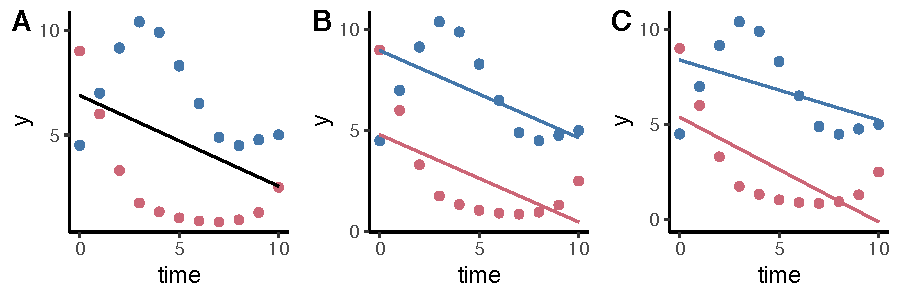
\includegraphics[width=3.9in, left]{Figures/methods/lm_plots.pdf}
    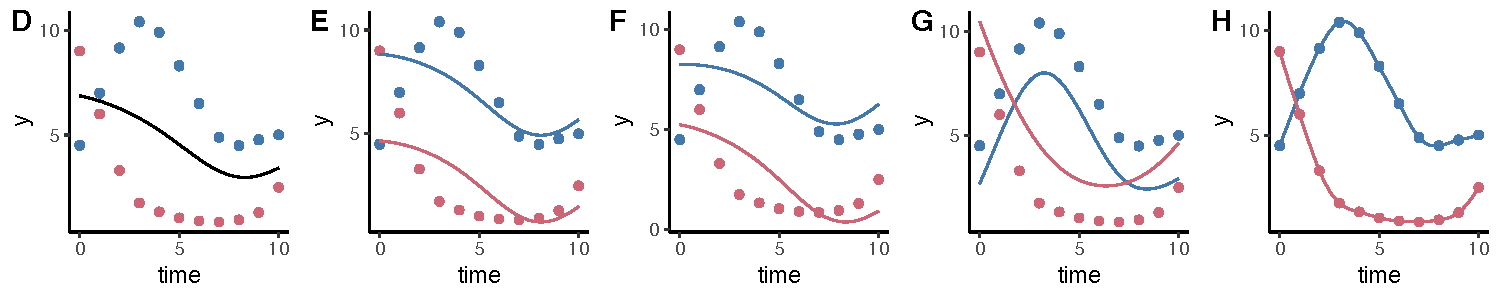
\includegraphics[width = 6.5in]{Figures/methods/gam_plots.pdf}
    \caption[Eight examples of regression models on the same data.]{Eight examples of regression models on the same data. Panels A, B, and C illustrate the capabilities of linear models and panels D, E, F, G, and H illustrate generalized additive models.}
    \label{fig:illustrative_gamms}
\end{figure*}

The lower panels of Figure~\ref{fig:illustrative_gamms} illustrate the effect of GAMs,\footnote{In this series of illustrative plots, I only use fixed effects and no random effects, so the model is simply a generalized additive model (GAM)---with one \textit{m}---rather than a generalized additive \textit{mixed-effects} model (GAMM).} specifically when smooths are added to the model specification. In the simplest model, time is included as a smooth term rather than a parametric term, which allows for a nonlinear best fit line (panel D). As with the linear models, the addition of group as a parametric effect allows for one line per group, though the lines are the same shape and are equidistant from each other at all time points (i.e., they’re parallel; panel E). Likewise, if an interaction term is included between time and grouping, the lines are allowed to have different slopes, but in this case the \textit{shape} of the curves are the same for both groups (panel F). When the group itself is included in the model as a smooth, but without any other parametric effects, the best fit lines for each group are different and resemble the original data, though they are constrained to occupy roughly the same vertical space (panel G). Finally, when group is added as a parametric effect in addition to being a smooth term, the \textit{position} of the lines is allowed to shift vertically, and the best fit line neatly lines up with the data (panel H).

This series of plots illustrates two several points when building a model. First, even the best linear regression model is inadequate to capture a nonlinear pattern in the data. Second, when fitting a GAM, it should include whatever grouping variable of interest as both a parametric effect and a smooth in order to allow to model fit different shapes and positions to the data. Finally, GAMs \textit{can} do an excellent job at fitting the data, but only when properly specified. The models illustrated in panels D--G fail to achieve the potential that a GAM has and are hardly better fits to the data than the linear models represented in panels A--C.

A detailed description of the mechanics of GAMs is out of the scope of this dissertation. For further explanation of generalized additive models (and their mixed-effects counterparts), I refer the reader to the many studies that have implemented these methods, as well as the sources cited within. For a tutorial on GAMMs on linguistic data, see \citet{soskuthy_2017} and \citet{wieling_2018}. Additional studies that implement these models on formant data include \citet{fruehwald_2017}, \citet{renwick_stanley_2020}, \citet{soskuthy_etal_2018}, \citet{warburton_2018}, and \citet{gahl_baayen_2019}. Linguistics studies that use GAMMs on other types of linguistic data include \citet{vanhofwegen_2017_diss}, \citet{kosling_etal_2013}, \citet{tomaschek_etal_2018_phonetics, tomaschek_etal_2018_vanguard}, \citet{strycharczuk_scobbie_2017}, and \citet{mielke_etal_2017}. And for a look at its underlying mathematics, see \citet{faraway_2016} and \citet{wood_2017}.

% TODO (Renwick): Q. some people, like Soskuthy, argue that using difference smooths to pinpoint where two trajectories are significantly different is a risky prospect. Why do you think it's a sound one? [I don't know how to address this because the crux of this dissertation hinges on this being a sound method.]
GAMMs can answer questions about a vowel trajectory that were previously not possible. For example, instead of ``How is the height/backness of \trap different between men and women?'', one could ask, ``How is the trajectory of \trap different between men and women?'' Similarly, one could analyze how a vowel changes shape across time, even if its relative position in the vowel space is the same across generations. Because GAMMs allow for detailed analysis of the full shape of the vowel’s curve (provided a sufficient number of measurements), one could even ask something like ``How does style affect the trajectory of \goose, and at what points along that trajectory is the difference statistically significant?'' Crucially, by analyzing the full trajectory of the vowel, researchers can uncover important linguistic differences that would otherwise not be found when analyzing the midpoints or some other static measure alone.

Why use GAMMs instead of one or more of the existing techniques that study the dynamic nature of vowels? Some studies have implemented techniques such as measuring the vector length, trajectory length, and spectral rate of change \citep{fox_jacewicz_2009, farrington_etal_2018, stanley_renwick_2019_LSA_poster}. Similarly, \citet{morrison_2013} outlines several additional methods that consider various properties of vowel inherent spectral change (the difference between the offset and the offset, the slope of the change, and the direction of change). The utility of these methods cannot be understated since important social patterns have been found to correlate with these measurements. However, they are based on measurements sampled at relatively few time points, and a ``higher resolution'' method can provide a clearer picture of the vowels' behavior. The critical difference boils down to the fact that these techniques allow one to study \textit{properties} of the trajectory while GAMMs allow for the study of the trajectory \textit{itself}. Ultimately, I believe listeners are sensitive to cues in the acoustic signal that are more nuanced than general properties like length and rate of change and that social variation exists in trajectory shape. While GAMMs may not be the ultimate best model to analyze vowel trajectories, they appear to currently be the best technique to uncover this variation.

\section{The implementation of GAMMs in this study}
\label{gamms_in_this_study}

With this background in mind, I now proceed to describe the statistical analyses used for studying the dynamic nature of vowels in the Elsewhere Shift in this sample. To get the most complete picture of the trajectory of a vowel in the F1-F2 space, I analyze their curved trajectories using GAMMs. By examining the model statistics, displaying predicted formant values, and comparing models with different predictor variables, I can identify which factors are influential in the overall shape of the curve. As will be shown hereafter, the use of GAMMs is justified because of the variation in trajectories that would have been overlooked when using single-point measurements alone.

\subsection{Model specificiation}

For each vowel class, I fit a GAMM to the Bark-transformed, normalized values of both F1 and F2 simultaneously in the same model. In most statistical modeling in linguistics, separate models are usually fit to F1 and F2. Sometimes, F1 and F2 are combined into a single measurement, such as the vowel's position along the front diagonal \citep{labov_etal_2013}. Instead, I follow the method used by \citet{gahl_baayen_2019} and \citet{renwick_stanley_2020} and restructure the data such that both F1 and F2 measurements are collapsed into a single \texttt{Hz} variable, which acts as the dependent variable in the model. A new variable, \texttt{formant}, is then included as one of the predictors that indicates whether that measurement is from the first or second formant. Table~\ref{tab:sample_table_wide} illustrates how the data might be structured when constructing a separate model for F1 and F2 and Table~\ref{tab:sample_table_tall} is the restructured data for a pooled model. So, for the main analysis, I fit a GAMM to the Hz measurement for all time points for both formants. This means that the model will take the 11 measurement points from which formants were extracted and essentially ``fill in the gaps'' to allow for a continuous model fit. Because information about what formant the measurement represents is included in the model, separate predictions are made for F1 and F2.

\begin{table}[t!]
    \hspace{\fill}
    \begin{subtable}[t]{0.35\textwidth}
        \centering
        \caption{Sample data, formatted as a ``wide'' table.}
        \liningnums{
            \begin{tabular}{c c c}
                word & F1 & F2\\
                \hline
                A & 1,650 & 600 \\
                B & 1,700 & 615\\
                C & 1,750 & 585
            \end{tabular}
        }

        \label{tab:sample_table_wide}
    \end{subtable}
    \hspace{\fill}
    \begin{subtable}[t]{0.35\textwidth}
        \centering
        \caption{Sample data, formatted as a ``tall'' table.}
        \liningnums{
            \begin{tabular}{ c c r }
                word & formant & {Hz\hspace{1em}}\\
                \hline
                A & F1 & 1,650 \\
                B & F1 & 1,700 \\
                C & F1 & 1,750 \\
                A & F2 &  600 \\
                B & F2 &  615 \\
                C & F2 &  585
            \end{tabular}
        }

        \label{tab:sample_table_tall}
    \end{subtable}
    \hspace{\fill}
    \caption{Two ways of organizing the same set of data. On the left is how FAVE output is formatted. On the right is the reshaped version used for analyses in this study.}
    \label{tab:sample_reshaped_data}
\end{table}

GAMMs are computationally intensive, so I aimed to keep the model specification as simple as possible while accounting for the sources of variation relevant to this study. For language-internal factors, only two variables were included: \texttt{duration} and \texttt{word}. \texttt{Duration} was included as a parametric effect only and it was log-transformed to make it more normally distributed. I include \texttt{duration} (interacting with the sociolinguistic factors as explained below) to allow the model to account for its effect, but it is not considered further in this study. \texttt{Word} was included as a random intercept only, but it was crossed with \texttt{formant} to give it different intercepts for F1 and F2, allowing the predicted trajectory to reposition itself freely in the F1-F2 space. No other phonological factor was included in the models.

Earlier versions of the models included information about previous and following segments. This was done in a host of different ways, such as including voicing and place and manner of articulation as parametric terms and the segment itself as a random effect. However, this model was grossly overspecified. Many combinations of factors were nonsensical for English data (a voiceless velar lateral, for example) and many pairings of previous and following segments were simply unattested due to accidental gaps in the lexicon (e.g. there are no English words with the sequence [\textipa{S\ae S}]). Fortunately, I was justified in removing all phonological factors for two reasons. First, I am not interested in consonantal effects within the defined allophones and I do not anticipate any meaningful variation to occur. But more importantly, whatever variation is captured by including phonological effects in the model is already accounted for (and more!) when word is included as a random effect (Baayen p.c.).\footnote{See \citet[47--48]{gahl_baayen_2019} who adopt the opposite approach and include surrounding segments as random effects rather than word. Either way, limiting the random effects structure is advised so as to avoid overfitting to the data.} So by only including word and duration in the model’s specification, the model was much simpler and had greater statistical and predictive power than an overspecified one with phonological factors also included.
In addition to language-internal factors, I included three variables related to language-external effects: \texttt{speaker}, \texttt{generation}, and \texttt{sex}. As was done with \texttt{word}, \texttt{speaker} was included as a random intercept only and crossed with \texttt{formant} to allow different intercepts per speaker per formant. My original intent was to include \texttt{age} as a continuous variable, rather than \texttt{generation}. I have already shown that language change in Cowlitz County has happened at a nonlinear rate \citep{stanley_2018_pwpl} and given that similar trends have been found in other communities \citep{fruehwald_2017}, I wanted to allow the model to account for a nonlinear rate of change in apparent time, specifically by including \texttt{age} as a smooth. However, this technique resulted in astronomical confidence intervals on the order of tens of thousands of Hz. As I explain in \S\ref{participant_metadata}, the age range in this data is spread over 69 years for just 54 speakers, which is spread thin given that men and women were modeled separately. I took these confidence intervals as a sign that a simpler approach was necessary to get trustworthy results with the current dataset. For this reason, I divided my speakers into generations and used that information in the model.

At the expense of model simplicity, I had theoretical reasons to include interactions between the two sociolinguistic variables (\texttt{generation} and \texttt{sex}). If they were included without any interaction, the model would allow for differences between the sexes and between generations, but the difference between the sexes would be the same in all generations. In other words, this would not be able to account for the possibility of language change happening in men and women at different rates. So, I modeled this interaction between \texttt{generation} and \texttt{sex} and included it both as a parametric effect and a smooth.\footnote{For the smooth, I used the \texttt{gam.check} function in the \texttt{mgcv} package to help determine the number of knots to use for the smooth. The maximum was 10 because I had data from 11 time points. After several tests, it was determined that four knots was sufficient to capture the shape of the curve without being overspecified.} This allowed the model to predict formant trajectories that were different in shape and position in the vowel space for both sexes in all four generations. However, to allow for independent curves for both formants in each of these combinations of factors, I actually had to create a three-way interaction between \texttt{generation}, \texttt{sex}, and \texttt{formant}. For example, if an observation is an F1 measurement from a baby boomer–aged woman, that information would be expressed as the string \texttt{F1\_F\_boomer} in the data. This interaction term had 16 such levels, representing the 16 combinations of \texttt{formant}, \texttt{sex}, and \texttt{generation}. Again, this comes at the expense of model simplicity, but I felt that it was important to allow all of these factors to vary freely.

Finally, the model controlled for autocorrelation between the residuals by including an AR1 residual error model. To do this, a model is fit without autocorrelation which is then used to calculate a value called rho. The rho value is then used in the calculations for the AR correlation in a second version of the model. (This original model is then discarded.) The following code was used to fit these models.\footnote{The crucial elements of this code block, which give the model the flexibility illustrated in Panel H of Figure~\ref{fig:illustrative_gamms} above, are the second and third lines.}

\begin{verbatim}
1  mdl_seed <- mgcv::bam(anae_barks ~
2                 formant_sex_gen +
3                 s(percent, by = formant_sex_gen, k = 4) +
4                 log(dur) * formant_sex_gen +
5                 s(word, formant, bs = "re") +
6                 s(speaker, formant, bs = "re"),
7              data = df, discrete = TRUE)
8  rho <- start_value_rho(mdl_seed)
9  mdl <- update(mdl_seed, rho = rho, AR.start = df$start_event)
\end{verbatim}


Using this template, identical models were then fit to each vowel class in this study. It took a little over two hours to run all models on my computer.

\subsection{Interpreting the GAMMs' output}
\label{sec:interpretation_of_gamms}

Determining whether a variable is significant\footnote{Around the time this draft was completed, \textit{The American Statistician} published a special issue called ``Statistical Inference in the 21st Century: A World Beyond \textit{p}~$<$~0.05''. This collection of 43 articles urges researchers to abandon traditional ideas of statistical significance: ``it is time to stop using the term `statistically significant entirely'' \citep[2]{wasserstein_etal_2019}. Though I still rely on confidence intervals in this study, which are ultimately derived from ``statistically significant`` \textit{p}-values, I do interpret these models with some care. Ultimately, I strived to heed to their advice: ``Accept uncertainty. Be thoughtful, open, and modest'' (ibid.).} in a GAMM is not as it is with other types of models. Because the three-way interaction variable is contained in the models both as a parametric term and as a smooth, it is not always straightforward to determine statistical significance from the model summary alone, particularly when the goal is to determine the significance of just one of those social factors. In particular, because of the way these interactions were implemented (i.e. a forced interaction by combining the constituent variables), lower-order terms were not included in the model.

For example, consider a hypothetical situation in which speaker sex was not relevant for some variable for this community. In a mixed-effects linear regression model fit with the \texttt{lmer} function in the \texttt{lme4} package \citep{bates_etal_2015_lme4}, I would create interaction terms by crossing the variables in the model formula itself (i.e. \texttt{sex * generation}). In the model summary, not only would I see the effect of this interaction, I would also see the effect of the factors themselves. If sex were not significant, neither interaction of \texttt{sex * generation} nor \texttt{sex} as an independent variable on its own would be statistically significant, but \texttt{generation} by itself would be. The model summary would lead me to conclude that \texttt{sex} may be removed from the model to create a better fit to the data. Unfortunately, such output is not possible with the current implementation of the \texttt{bam} function in \texttt{mgcv} \citep{wood_2017} so testing the effect of one of the variables in the interaction is not possible with the model's output alone.

Fortunately, the significance of a variable can still be tested by fitting two models---one with the variable (the ``full'' model) and one without (the ``base'' model)---and comparing their fit to the data. If the inclusion of that predictor improves model enough to justify the extra complexity, it is considered a significant predictor. (This method is also used to test the significance of predictors in linear regression or linear mixed-effects models.)

In all cases though, \texttt{formant} was retained in the ``base'' models because I always expect significant differences between F1 and F2 regardless of the social factors in the model. These comparisons were made using the \texttt{compareML} function in the \texttt{itsadug} package \citep{van_rij_etal_2017_itsadug}.\footnote{Note that comparison of models that include the AR1 model make the AIC scores unreliable, but the significance tests can still be trusted (Renwick, p.c.). } For all vowels, the model comparisons suggest that the inclusion of sex and generation significantly improve the model fit (Appendix~\ref{appendix:model_comarisons}, so their output will not be described in much detail in the results chapters.

%However, because the predictors were included in the model only as part of a three-way interaction term, the comparison is not simply between a full and base model. Instead, all possible subsets of the three-way interaction are created and separate models are fit with those lower-order interactions (Figure~\ref{fig:model_nesting}).

%\begin{figure}
%    \centering
%    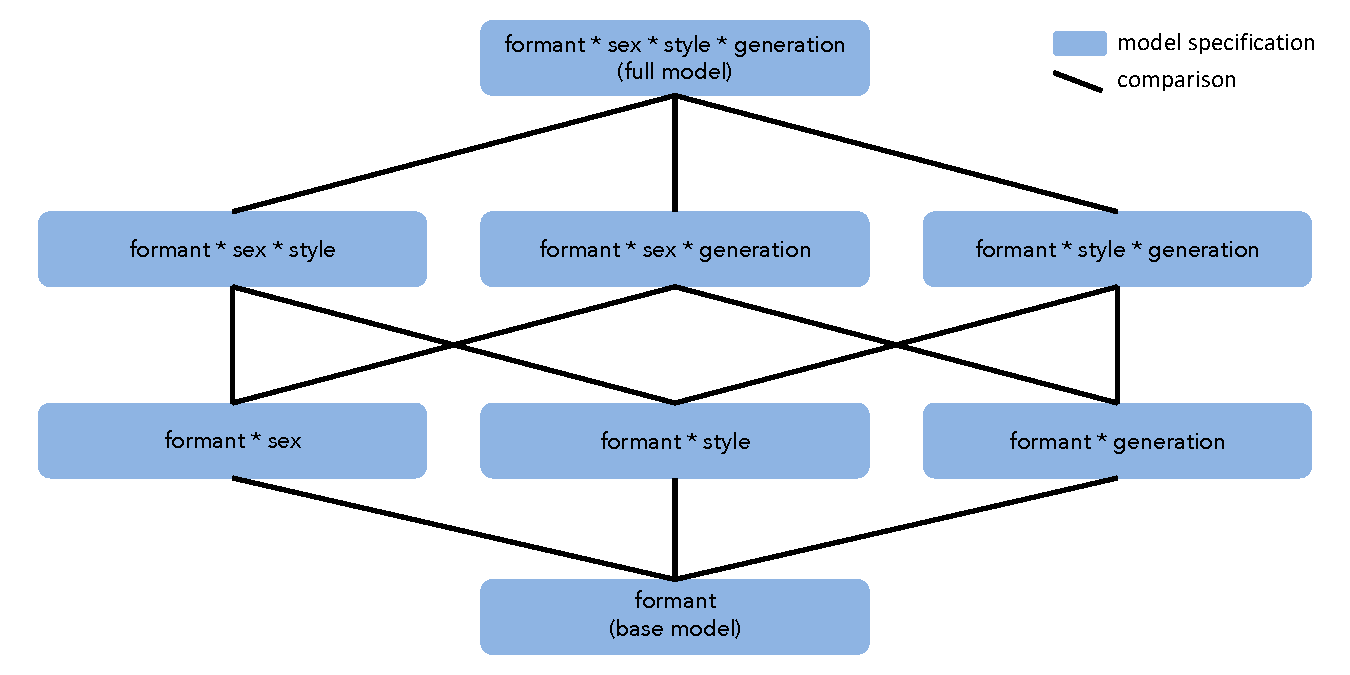
\includegraphics[width=\textwidth]{Figures/methods/subset.pdf}
%    \caption[A visualization of the models created for each vowel.]{A visualization of the models created for each vowel. Boxes represent models and lines connecting them represent one comparison test that was implemented. Incidentally, parallel lines indicate the addition of the same variable: all vertical lines connect models that differ only by the addition or removal of style and test for its significance, diagonal lines from bottom left to top right test for generation and diagonal lines from bottom right to top left test for sex. Theoretically, if a variable has absolutely zero correlation with the depedent variable, the model comparison tests that the parallel lines represent would not be statistically significant.}
%    \label{fig:model_nesting}
%\end{figure}

%Imagine again a scenario in which style is not a significant factor in the data, but it is still included in the four-way interaction. This full model (labeled A in Figure~\ref{fig:model_nesting}) is compared against a model that does not account for style whatsoever with only a three-way interaction between formant, sex, and generation are included (B). In the model comparison (line a-b), the simpler model without style (B) would be considered the better fit to the data because it accounts for the same amount of variance with a less complex model specification (A). However, in this scenario, imagine that generation is a significant predictor: a model that contains only a three-way interaction between formant, sex, and style (C) would perform worse in comparison (a-c) to the full model (A) because the larger model accounts for much more of the variation. This is seen in the output of the model comparison and is justification for including generation in the model. But, as additional support that style is not a significant predictor, the model with the three-way interaction of formant, sex, and style (C) would also be a worse fit than one with a two-way interaction between formant and sex (neither style or generation are in this smaller model; D; c-d) because whatever variance the three-way interaction can account for, the two-way interaction can also explain it with less complexity.

\section{Visualizing the GAMMs' predicted values}
\label{sec:visualizing_gamms}

While these model comparisons helps determine a variable’s significance in the model, it does not help the analyst understand what kind of effect it has on the shape of the curve. And because of the non-linear effect the variables have on the predicted values, the coefficients of predictors by themselves are largely uninterpretable by any analyst because they do not indicate anything about the shape of the curve. Therefore, a visualization of the predicted values is provided to clarify how the model was fit to the data. They also provide a useful way to show trajectory data. The authors of the \textit{Atlas of North American English} describe the difficulty in visualizing trajectory data:
\begin{quote}
    ``While it is easy to plot an array of sequential measurements of a single vowel, plotting 300 such trajectories for a single speaker would obscure any pattern and preclude the goal of describing the vowel systems of North America'' \citep[38]{labov_ash_boberg_2006_anae}.
\end{quote}
Essentially, a visualization of all the raw trajectory data in the F1-F2 space looks like a bowl of spaghetti and the patterns are impossible to discern. The predicted values from a GAMM consolidate vowel tokens and groups of speakers into a single line. Therefore, visualizations of these predicted values allow for a consolidated view of the data, relatively free from the noise and messiness inherent in data extracted using automatic means.

I therefore present model visualizations in three primary types of multi-panel plots: F1-F2 plots, spectrogram-like plots, and difference smooths.

\subsection{F1-F2 plots}

\begin{figure*}[tb!]
    \centering
    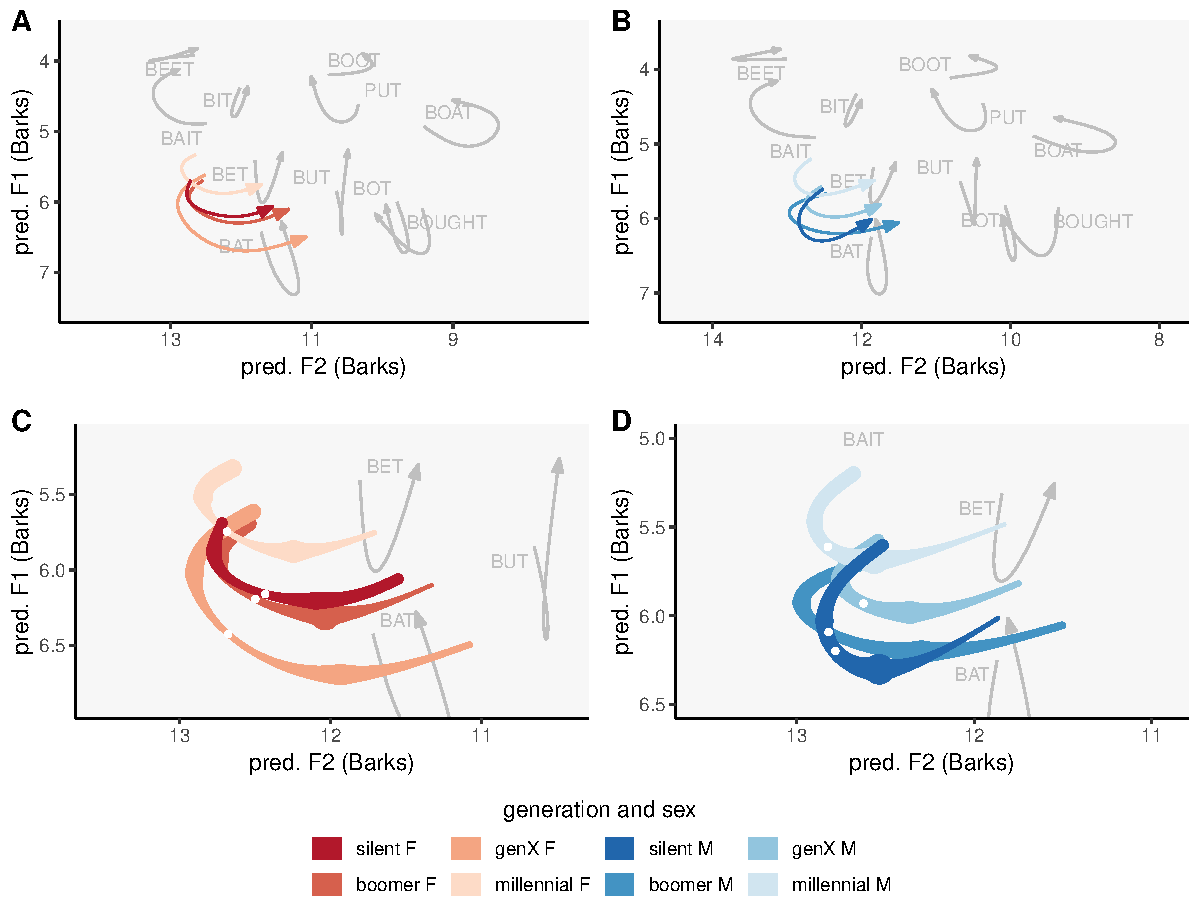
\includegraphics[width = 6.5in]{Figures/BAN/BAN_four_panel_plot.pdf}
    \caption[A sample four-panel plot used in this dissertation.]{A sample four-panel plot used in this dissertation. This shows the \ban vowel and is explained in more detail in \S\ref{BAN}.}
    \label{fig:sample_four_panel_plot}
\end{figure*}

In the results chapters, I present model visualizations in a series of four-panel plots, each displaying different views of the predicted values in the F1-F2 space. Figure~\ref{fig:sample_four_panel_plot}, taken from \S\ref{BAN}, is an example of such a plot. All images display a set of curves in color, representing the predicted values for the vowel in question. Another set of curves is underlayed in gray and represent the predicted values for all vowels\footnote{The underlaid trajectories represent elsewhere allophones of the other vowels too. Prelateral and prerhotic tokens are not included when calculating these trajectories. Furthermore, post-cororanl tokens of \goose and \goat were excluded to form the \boot and \boat allophones.} in the entire community as a point of reference. All plots are in the Bark-transformed, normalized F1-F2 vowel space. Panels A and B (on the top) offer a ``zoomed out'' view, allowing the viewer to examine the trajectories in relation to other vowels and to see their position in the vowel space. Panels C and D are ``zoomed in'' to facilitate viewing the shapes of the curves themselves. The data presented in the left two panels (A and C) are identical and always show the women’s data in shades of red. Likewise, the two panels on the right (B and D) display the men’s data, which is identical between the two panels, in shades of blue. On the top two plots, a small arrow has been placed on the offset of the vowels to indicate the direction of movement. The thickness of the lines in the bottom two panels corresponds to the rate of change, with thicker portions representing little movement, and narrow portions showing fast change, as if they were drawn with a quill pen.\footnote{For the curious, I am not aware of a way to get a continuous change in line thickness in \texttt{ggplot2}. I pulled off this effect by extracting predicted values at 501 equally spaced intervals along the vowels' duration (0.2\% intervals) and plotted them as points. The size of the circles reflects the euclidean distance from the previous point. Because so many points are all plotted so closely, the effect is a smooth line that changes width. I credit \citet{fruehwald_2017_gamm} for the idea for these plots.} Furthermore, on the bottom two plots, a small white dot has been placed on the midpoint of the vowel, illustrating what information would have been gleaned had only single-point measurements been used in this study and to facilitate comparison with previous studies.

These plots contain a wealth of information about the predicted values of these GAMMs. Their interpretation is facilitated by the fact that each set of four-panel plots is formatted and sized identically throughout this dissertation,\footnote{To ensure all the plots are identically formatted, I wrote a custom R function that takes in a GAMM and produces the full four-panel image.} so once the reader has learned to read one, they will be able to read them all. The only thing that changes from plot to plot is the data being displayed, and the axes of the bottom plots (the axes on the top two are fixed).


\subsection{Spectrogram-like plots}

\begin{figure*}[tb!]
	\centering
	%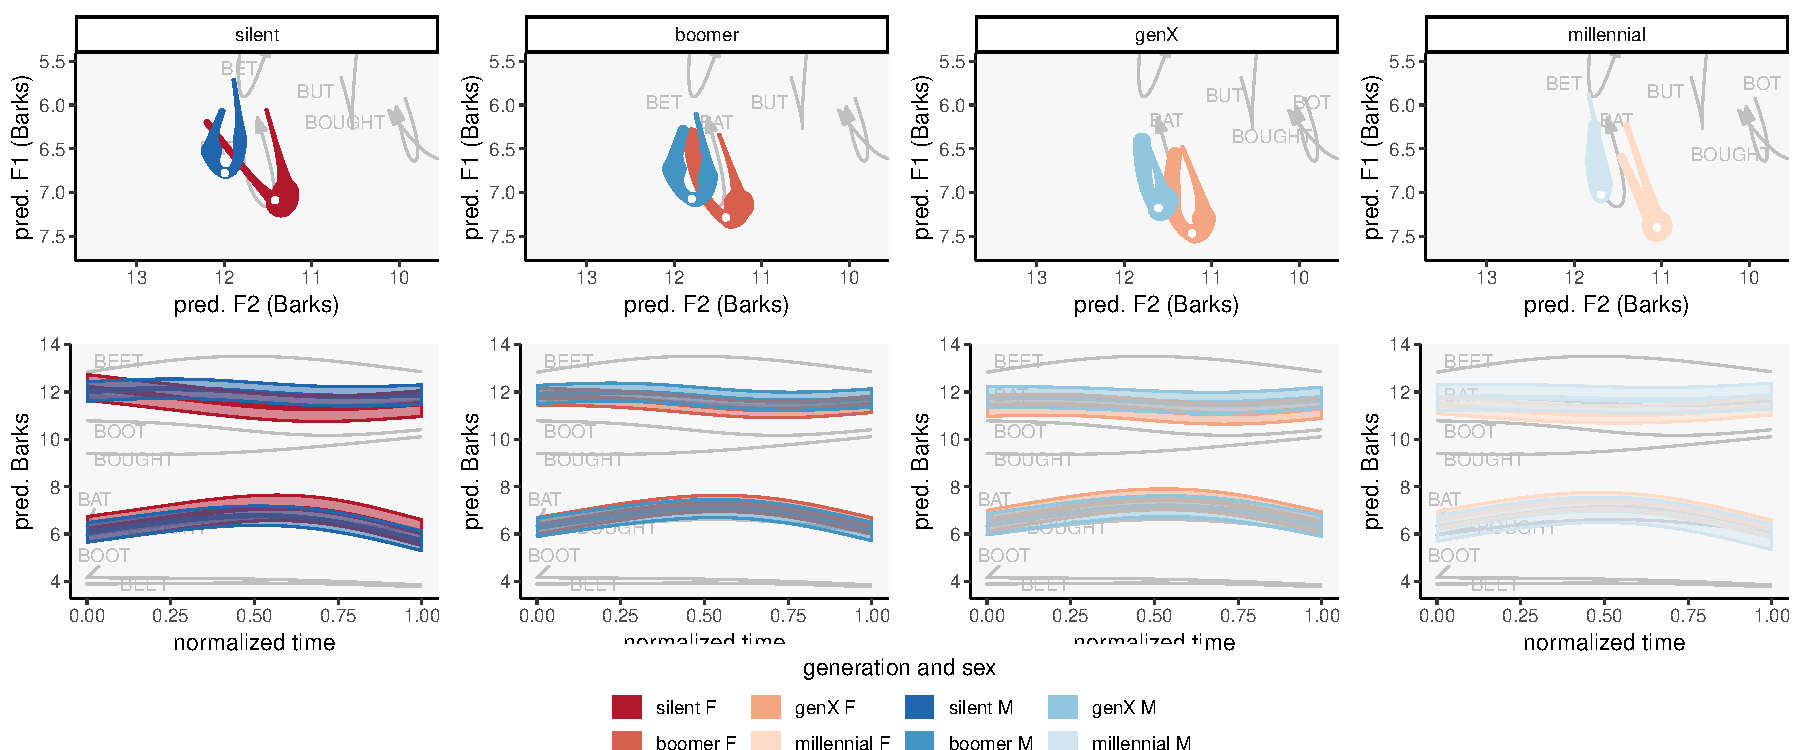
\includegraphics[angle = 90, origin = c, height = 6in]{Figures/BAT/BAT_sex_panel_plot_wide.pdf}
  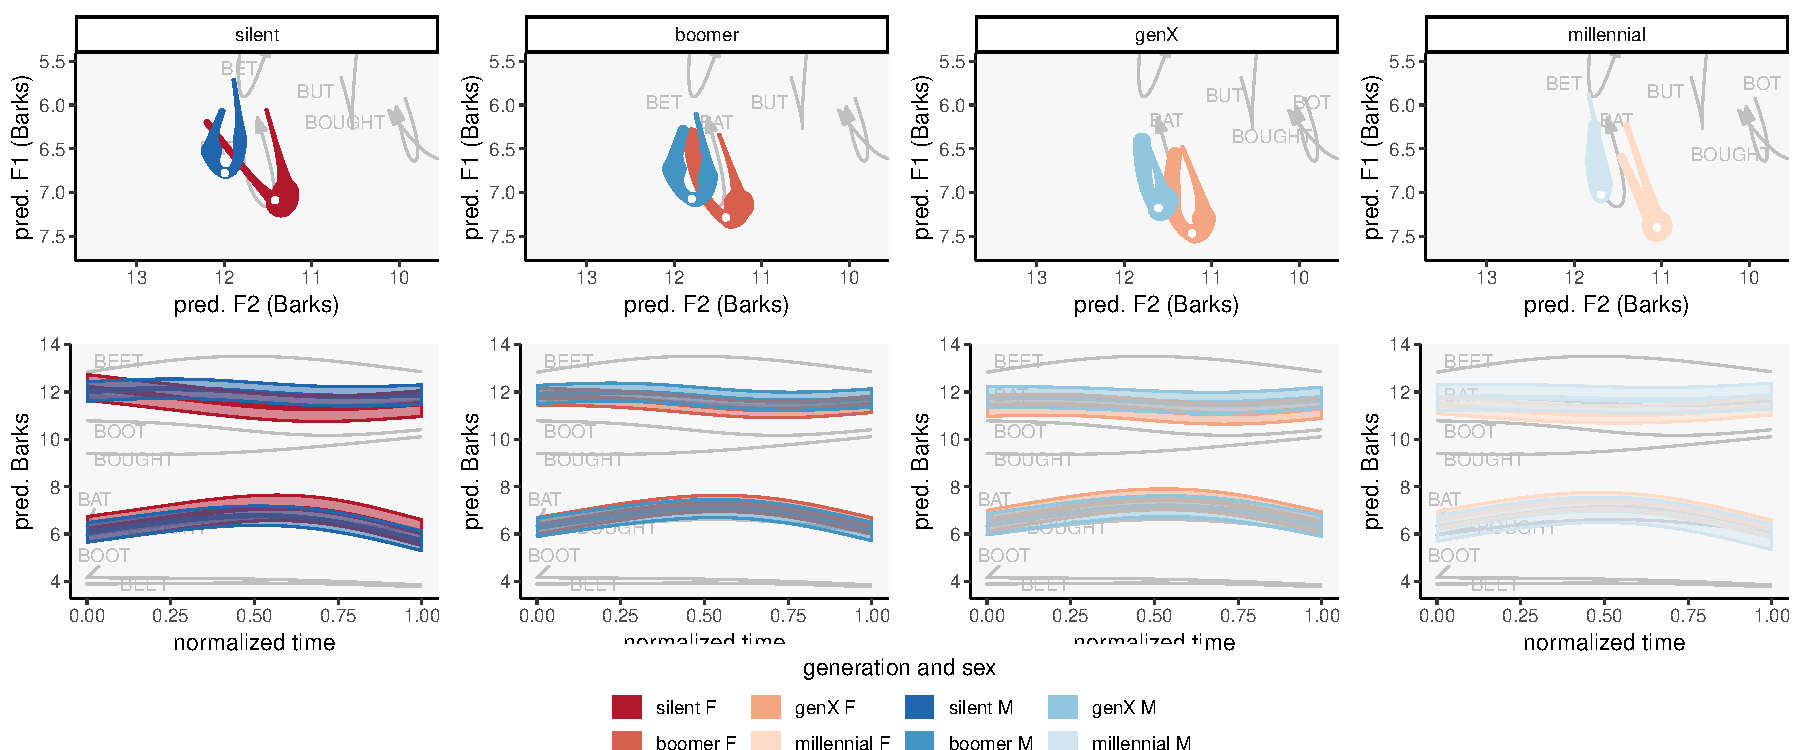
\includegraphics[width = 6.5in]{Figures/BAT/BAT_sex_panel_plot_wide.pdf}
	\caption[A sample eight-panel plot used in this dissertation.]{A sample eight-panel plot used in this dissertation. This shows the \ban vowel and is explained in more detail in \S\ref{BAN}.}
	\label{fig:sample_spectrogram_plot}
\end{figure*}

As an alternative view of the data, I also present the formant trajectories in plots that are reminiscent of spectrograms. By this, I mean that time is along the \textit{x}-axis and formant frequency (in Barks) is along the \textit{y}-axis. These should be familiar to those comfortable with viewing spectrograms in programs such as Praat.

Figure~\ref{fig:sample_spectrogram_plot} is an example of a series of plots that uses these spectrograms. In this layout, the four generations are split up, with the oldest generation on the left and the youngest generation on the right. The top four panels show predicted formant values in the F1-F2 space, just as they are displayed in the other F1-F2 plots, with the difference being that men and women are plotted together, but only from one generation.

Underneath these plots are the spectrograms. The \textit{x}-axis, going from left to right, represents normalized time, with the vowel onset on the left edge and the offset on the right edge. The lower two bands represent F1 and the upper two represent F2, with women in shades of red and men in shades of blue. For ease of interpretation between the different plots, the colors and shades are identical with those in four-panel plots described in the previous section.\footnote{It was difficult to find four shades that worked harmoneously together while being able to stand out against a white background. Consequently, the colors used for the Millennials are admittedly a little too faint. Unfortunately, due to COVID-19, I was unable to return to campus to retrive my data, meaning I could not rerun the models and reproduce the visualizations in time for this dissertation to be submitted.} Like the F1-F2 plots, faint gray lines are underlaid to show what the predicted formant trajectories were for four corner vowels, to show the extremes in formant frequencies.

\subsection{Difference smooths}

Finally, the last type of visualization used in this dissertation are a special kind of output called \textit{difference smooths}. Since these are only used in Appendix~\ref{appendix:difference_smooths}, a detailed description of how to interpret those plots is found there.

\subsection{A typology of formant curves}

Because relatively few sociolinguistic studies have analyzed formant curves in the F1-F2 space in depth, we lack the terminology needed to describe the shape of these curves. In this section, I propose five types of formant curves, which are illustrated in an idealized form in Figure~\ref{fig:curve_types}. The top panels represent what these curves would look like in the F1-F2 space while the bottom panels show what the formant movement would look like in a spectrogram.

\begin{enumerate}
  \item \textit{The Line}---This is the most basic formant shape, the onset is in one point in the vowel space, the onset is in another, and the trajectory connects the two in a straight line. When oriented horizontally as in Figure~\ref{fig:curve_types}, there is no formant movemement in F1. Note that an analysis that extracts formant measurements at only two timepoints will result in all vowels being of this type, which may be a simplication of a more complex underlying curve. If however additional measurements are taken and the trajetory is still a line, then it may be said that that vowel has this shape.
  \item \textit{Bounce}---In the F1-F2 space, the Bounce appears to move from one point to another and then back in a straight line. When oriented vertically as it is in Figure~\ref{fig:curve_types}, F2 is constant throughout the duration of the vowel. F1, meanwhile, ascends and then descends.\footnote{It is probably of little consequence whether the rate of change in F1 is constant. The F1-F2 plot would look the same regardless (unless rate of change is incorporated into the visual), though a spectrogram would reveal a more curved arc rather than a jagged point.} The point of inflection in F1 is clear and would presumably be the target of the vowel. An analysis that extracts measurements at only three timepoints may find a Bounce in all vowels, so data from additional timepoints are necessary to identify whether a trajectory is truly a Bounce.
  \item \textit{The V}---The V is similar to the Bounce, only there is (presumably constant) movement in F2 over the course of the vowel's duration.\footnote{Obviously the Bounce and the V represent points along a continuum and in some cases a curve will fall somewhere between the two.} The target is still clearly defined as the point of inflection in F1. The V and Bounce can each be described as ``pointy'' trajectory shapes, reflecting the abrupt reversal in F1 and clear point of inflection in the F1-F2 space. Like the Bounce though, the V will be common, if not the norm, in a three-point analysis and only after extracting measurements from more timepoints will an underlying V shape be revealed.
  \item \textit{The U}---Adding complexity to the V, the U introduces a smoother formant movement than the two ``pointy'' shapes described above. In this example, F2 still descends at a constant rate and while F1 does ascend and descend like the Point and the V, it does so more smoothly than in the V. In the F1-F2 space, the U still has a target, though it is less clearly identifiable; there is no steady state in U-shaped trajectories.
  \item \textit{The Bowl}---Like the other shapes, F1 rises and falls in the Bowl trajectory shape, but unlike the other types, there is no clear inflection point. In both the F1-F2 plot and the spectrogram, there is no easily identifiable target. In the spectrogram, the rate at which F1 increases decelerates to a point where there is almost a flat formant trajectory for a brief time,\footnote{Similarly, a bowl is flat on the bottom so it can rest on a table.} after which F1 slow begins to lower again, picking up speed towards the ends of the vowel's duration. In the Bowl, the point of inflection in F1 is somewhat arbitrary and, as suggested in the F1-F2 plot, it is unclear if that point would actually represent a target. Instead, the F1-F2 suggests that there are two targets in a Bowl, one corresponding to each of its ``corners'', though it is unclear what the acoustic correlates of these corners might be (or indeed how to identify them in the spectrogram).
\end{enumerate}

\begin{figure*}[tb!]
    \centering
    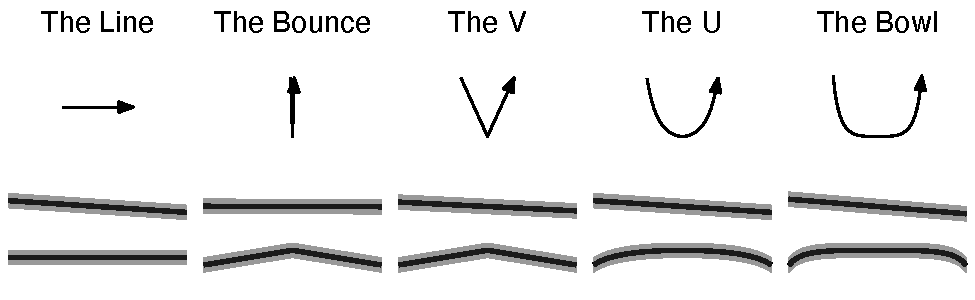
\includegraphics[width = 6.5in]{Figures/other_figures/traj_shapes.pdf}
    \caption{Five types of formant curves}
    \label{fig:curve_types}
\end{figure*}

These descriptions, especially the particulars of the formant movements, are based on the idealized versions of these trajectories displayed in Figure~\ref{fig:curve_types}. In reality, the data will be messier. For example, any of these trajectories can be rotated to an arbitrary angle. If the formants swap roles (e.g., F1 changes at a constant rate while F2 has a curved shape in the U), then the curve will appear sideways in the F1-F2 plot. If F2 lowers gradually rather than raises, the direction of movement will go the opposite way (and visually, the arrow will be on the other end), creating ingliding or offgliding variants. In this study, if a trajectory has an offset with a lower F2 than the onset (as in Figure~\ref{fig:curve_types}, depicted visually with the arrow on the right), I often call it \textit{right-hooking} (or ingliding since I deal primarily with front vowels). For trajectories that go the opposite way, I call them \textit{left-hooking}.

\begin{figure*}[tb!]
    \centering
    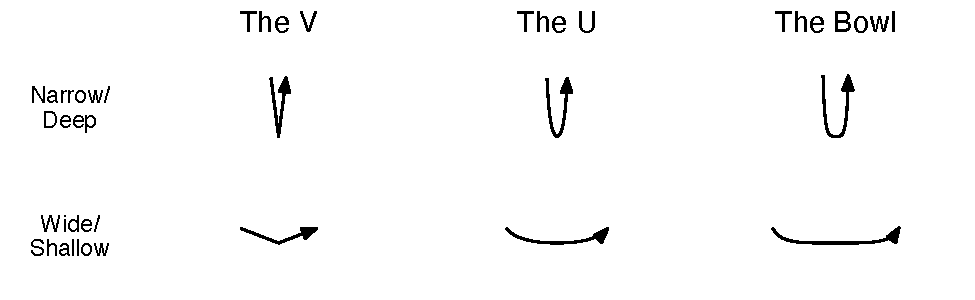
\includegraphics[width = 6.5in]{Figures/other_figures/traj_shapes_mod.pdf}
    \caption{Modified versions of the formant types.}
    \label{fig:curve_types_mod}
\end{figure*}

It may be helpful to modify the terms with adjectives to describe the amount of change in one formant relative to the other (\ref{fig:curve_types_mod}). For example, a Bounce is essentially a very \textit{narrow} V, meaning that F1 changes much more relative to F2. Alternatively, a very \textit{wide} V would have much more change in F2 than in F1 and may even approach the Line. One may also find narrow and wide U and Bowl shapes as well. Alternatively, the terms \textit{deep} and \textit{shallow} may be used, perhaps synonymously with \textit{wide} and \textit{narrow}. To be clear, the Bowl is not simply a wide U because the Bowl has two inflection points and the U has only one; however, a narrow Bowl may be simply described as a U because there is likely little need of describing two very close inflection points.

The point is that these labels are primarily descriptive and are not necessarily meant to represent differences in how formant trajectories are stored at the cognitive level.\footnote{However, it could be tested experimentally whether listeners discern differences between these formant shapes.} The difference between a Bounce and a narrow V and between a U and a Bowl can be subjective. The difference between a Line and a very shallow V or U is not clear either. For now, I present these terms to ease descriptions of formant trajectories in this study.

Finally, these terms were developed based on the data analyzed in this dissertation and, perhaps more importantly, upon the analysis used. Since these GAMMs fit curves with only 4 knots, there can only be so much wiggliess in the resulting shape. A triphthong likely exhibits additional complexity that four knots (and these five descriptive terms) cannot handle. Therefore, while these terms may be useful to other researchers who study formant movement, it is not a closed class of labels.







\section{How to identify and quantify vowel shift}
\label{how_shifting_is_measured}

After the GAMMs have been fit to the data, the final step in the analysis is to actually determine whether the vowels have shifted in apparent time. In this section, I describe methods used to determine whether vowels have shifted and weigh their pros and cons. I ultimately choose to simply compare younger generations to older generations in this community.

\subsection{Method I: Relative position from an anchor vowel}

In general, in order to show that vowels change is to do so in relation to some stable or anchor vowel \citep[103--104]{dipaolo_etal_2011}. For example, the height of \trap is often compared against that of \lot \citep[20]{thomas_2001}. Lowering of \bit is sometimes determined by comparing its F1 to \face's F1 (\citealt[44]{kennedy_grama_2012}, \citealt[97]{bowie_2017_pads}). In a large sample including Canadians and Americans, \citet{boberg_2019} finds that \kit has shifted lower than \face and that \trap is further back than \goose and is close to the nucleus of \mouth. These are useful measurements, especially considering that vowel’s canonical positions are generally known.

However, in Western American English, all vowels are undergoing a change of some sort: \kit, \dress, and \trap are lowering and/or retracting as part of the Elsewhere Shift, the merged \lot-\thought vowel is raising and backing, and all other back vowels are fronting. Of the remaining vowels, \fleece is lowering and retracting in California \citep{donofrio_etal_2019} and \face is more monophthongal in Washington than elsewhere in the West \citep{wassink_2015}, so their usefulness as reference points would vary across the West. Thus, a description of one vowel in relation to another is potentially problematic in Western American English.

Nevertheless, the stable position of \fleece in other areas is perhaps the motivation for the development of a unitary measure of the Elsewhere Shift: the \textit{Short Front Vowel Shift Index} \citep{boberg_2019}.\footnote{This method is also used by the various authors in the recent volume on the Elsewhere Shift \citep{becker_2019_pads}.} This index is calculated as the average Cartesian distances between \fleece-\kit, \fleece-\dress, and \fleece-\trap, using mean values for each vowel. A similar method was adopted by \citet{holland_2019}, \citet{pratt_donofrio_2017}, and to some extent \citet{podesva_etal_2015}. One benefit of this multivariate measure is that it gets away from a strict separation of the F1 and F2 dimensions \citep{becker_2019_pads}. However, a measure that reduces the shifts of three vowels down to a single number may make sense for versions of the Elsewhere Shift in which the three are retracting in parallel at the same time. But if the vowels are more independent, such as what is found in this study, this single number may not be the most appropriate way to measure the Elsewhere Shift.

% TODO Read Kendall & Fridland 2017 (LVC) for measures from BOT. Also, Swan (2019).

\subsection{Method II: Comparison against \textit{ANAE} benchmarks}

What is needed is some stable reference value to compare formant measurements against. These reference values would presumably measure what a conservative or innovative vowel might be, and measurements in relation to these benchmarks would determine the degree of shifting. The closest thing to these benchmarks are the values used in maps of the \textit{Atlas of North American English}. For example, in a map that illustrates the Canadian Shift (Map 15.4, page 219), speakers are coded as either having the Canadian Shift or not. Given their average measurements per vowel, if a speaker’s F1 for \dress was greater than 660, F2 for \trap was less than 1825, and F2 for \lot was less than 1275, than they were coded has having the Canadian Shift. Speakers that did not satisfy all three of these requirements were considered to not have the shift. This way of determining the presence of the shift was useful in the construction of that map, which showed a high degree of homogeneity among Canadian speakers.

These values have since been used as benchmarks to determine whether \lot, \trap, or \dress are retracted or lowered. For example, \citet[44]{kennedy_grama_2012} state that ``subjects meet the definition of the Canadian shift if they have (1) F1 of \dress greater than 650 Hz, (2) F2 of \trap less than 1825 Hz, and (3) F2 of \lot less than 1275 Hz.'' Similarly, \citeauthor{becker_etal_2016_pads} use these values and state that ``[v]owels which cross these cut-off points are considered shifted'' \citeyearpar[113]{becker_etal_2016_pads}. Similar methods are also adopted in studies on the Elsewhere Shift in New Mexico \citep{brumbaugh_koops_2017_pads} and Utah \citet{bowie_2017_pads}. Thus, it appears that though all vowels are shifting in the West, these benchmarks satisfy the need for stable, reference values to measure the Elsewhere Shift.

However, it does not appear that these numbers were intended to be used for that purpose. For one, these numbers only appear in the \textit{ANAE} maps' legends and are not mentioned in the text. Furthermore, they are different from map to map: Map 11.7 (page 132), which also shows the Canadian Shift, has the F1 threshold for \dress as 660 Hz instead of 650 Hz. And though the cutoff for a shifted \trap was 1825 Hz, the mean F2 for Canadian speakers’ realization of \trap was 1725 Hz. These are admittedly small differences, but they illustrate that the cutoff values are not absolutely fixed. If these numbers were intended to be important benchmarks for determining degree of shifting, should they be not consistent from map to map, perhaps presented in a table in the text itself, and described in detail as to how and why those particular values were determined?

Instead, it appears that these numbers were used solely for the purpose of creating the isoglosses for the maps. F1 and F2 are continuous measurements, so it is somewhat meaningless to divide the range of values into ``shifted'' or ``not shifted.'' Nevertheless, this binary split was necessary because the method used for determining isoglosses was an iterative process which sought to maximize either the homogeneity of speakers within a determined region or the proportion of speakers that have a particular linguistic feature. After an isogloss is drawn, it was evaluated and altered until it converged on an optimal dialect boundary. As part of this altering process, the cutoff value for determining the presence or absence of a linguistic feature could be modified if it resulted in a better fitting isogloss: ``one may adjust this value to maximize either homogeneity or consistency'' \citep[43]{labov_ash_boberg_2006_anae}. Thus, the benchmarks were allowed to vary from map to map (as in Map 11.7 and Map 15.4) to produce cleaner isoglosses. It does not appear to be the case that these numbers are meant to be absolute cutoff values that determine presence or absence of a vowel shift in a theoretical way. Instead, it appears then that these arbitrary benchmarks were calculated to be the best for maximizing homogeneity and drawing an isogloss around the most consistent group of speakers within that dataset.

Therefore, treating these values as strict benchmarks can be potentially problematic when speakers who are expected to shift do not meet the qualifications. \citeauthor{kennedy_grama_2012} find that their sample of California-based speakers passed the threshold for \dress lowering and \trap retraction but that they ``cluster around'' the threshold for \lot retraction \citeyearpar[49]{kennedy_grama_2012}. This is their primary support for the Canadian Shift and California Shift being independent processes and for the low back merger not necessarily being the trigger of \trap retraction. Furthermore, the arbitrary threshold divided their speakers into those with vowels similar to those in the Canadian Shift and the ``remaining subjects [who] are somewhat of a mystery'' \citeyearpar[51]{kennedy_grama_2012}. Treating these benchmarks as general guidelines instead of absolute cutoffs may reduce the need for dividing a somewhat homogeneous cluster into two groups.

Finally, \citet{dinkin_2018} points out that in order to appropriately apply these benchmarks to a new dataset, the data must be normalized using the same procedure as the one used in the \textit{Atlas of North American English}. Because the units of these benchmarks are in Hz, it is not immediately apparent that the data are normalized and that similar techniques are required to apply a meaningful interpretation onto a new dataset. With what is probably the most popular normalization procedure in sociolinguistics, the \citet{lobanov_1971} transformation converts F1 and F2 values into z-scores (i.e. number of standard deviations from the mean values). For researchers who use FAVE, which may be the most common method for formant extraction in North American sociolingustics, these z-scores are then rescaled so that F1 has a mean of 650 Hz with a standard deviation of 150 Hz and F2 has a mean of 1700 Hz and a standard deviation of 420 Hz. Thus, the methods used by FAVE and by the \textit{Atlas of North American English} produce values that are Hz-like and are in the expected ranges. But comparing results from one method with another (or against raw measurements) is like comparing apples to oranges. \citet{dinkin_2018} explains that the differences may seem superficial, but a reanalysis of his data shows that the F1 of some speakers’ \trap vowel is below the \textit{ANAE} benchmark of 1825 Hz when using one method and above it when using the other. In other words, conclusions drawn about the degree of shifting can entirely depend on using the proper normalization procedure when comparing to the \textit{ANAE} benchmarks.

\subsection{How shifting is measured in this study}

In this section, I have discussed the need for some sort of stable reference values to measure the degree of shifting and have critiqued the use of the \textit{ANAE} benchmarks to serve this purpose. To my knowledge, there are no other reference values that have been used to show whether the front lax vowels are shifting. To complicate matters even more, how should such a benchmark be treated when vowel dynamics are considered? Does the entire trajectory need to be past the cutoff value or is just one measurement sufficient? If some proportion of the trajectory should be past the benchmark, how does one determine the amount? To my knowledge, there really is no agreed-upon way to objectively measure the degree of shifting across studies.

For now, the best solution---and the method that I use in this study---is to focus on one vowel and compare the realizations used by two different groups. In other words, the most effective way for analyzing shift in apparent time is by comparing older people to younger people in the same community \citep{boberg_2005, cardoso_etal_2016_pads, holland_brandenburg_2017_pads, hall_lew_etal_2017}. Comparing pronunciations by different genders and ethnicities \citep{brumbaugh_koops_2017_pads} can also help determine the relative amount of shifting between groups. When visualizing the vowel space, it is also be ideal for other vowels for these groups of speakers to also be plotted, partially as reference values, but also to give an idea of the degree of shifting, with the understanding that these reference vowels may also be changing in time. This method for gauging how much shifting is occurring is not entirely satisfactory because it makes it impossible to determine whether one community is more shifted than another. Nevertheless, this is the method used in this study and I leave it to future work for determining a more objective way for comparing the shift across studies.

\section{Hardware and software}
\label{r_packages}

Data processing and analysis for this study was done using version 3.5.1 of R programming language \citep{r_2018} using version 1.1.463 of the RStudio software. In addition to the many functions that come with the standard distribution of R, I relied heavily on these packages:

\begin{itemize}
    \item The bulk of data processing, transformation, and cleanup was done using the various packages in the \texttt{tidyverse} \citep{wickham_2017_tidyverse} including \texttt{readr} \citep{wickham_etal_2018_readr}, \texttt{readxl} \citep{wickham_bryan_2019_readxl}, \texttt{dplyr} \citep{wickham_etal_2019_dplyr}, \texttt{tidyr} \citep{wickham_henry_2018_tidyr}, \texttt{stringr} \citep{wickham_2019_stringr}, and \texttt{forcats} \citep{wickham_2019_forcats}.
    \item To manage the many models in this study, I used \texttt{modelr} \citep{wickham_2019_modelr} and \texttt{broom} \citep{robinson_hayes_2018_broom}.
    \item The models themselves were run using \texttt{mgcv} \citep{wood_2017} and the predicted values were extracted using \texttt{itsadug} \citep{van_rij_etal_2017_itsadug}.
    \item All visualizations were done in \texttt{ggplot2} \citep{wickham_2016_ggplot2} with the help of \texttt{ggrepel} \citep{slowikowsky_2018_ggrepel} for vowel labels. They were combined into the four-panel plots using \texttt{cowplot} \citep{wilke_2019_cowplot}.
    \item All non-gray colors in the visualizations are from Paul Tol's \citeyearpar{tol_2012} color schemes, accessed via \texttt{ggthemes} \citep{arnold_2018_ggthemes}.
\end{itemize}
The hardware was an early 2014 model MacBook Air running macOS 10.14 (Mojave). The bulk of processing was done in late 2018.

% Praat
% QGIS plus data sources
% LaTeX
    % 15,298 words
\clearpage\chapter{The elsewhere allophones of the front lax vowels}
\label{ch:elsewhere_shift}

This chapter presents a description of the elsewhere allophones of the front lax vowels in Cowlitz County. Recall that these allophones of \trap, \dress, and \kit, are those that occur before obstruents (except /\textipa{g}/) and are most directly related to the Elsewhere Shift. \S\ref{BAT}--\ref{BIT} discuss the \bat, \bet, and \bit vowels, respectively, primarily based on visualizations of the model outputs for each vowel. In \S\ref{sec:preobstruent_discussion}, I summarize the findings and conclude the chapter with a brief discussion of the implications of these results. A more in-depth discussion of these findings, particularly as they relate to speakers' relationship with the Pacific Northwest and the mills, is presented in Chapter~\ref{ch:discussion}.

% ---------------------------------------------------------------------------------
% ------------------------------    BAT    ----------------------------------------
% ---------------------------------------------------------------------------------

\section{\bat}
\label{BAT}

In this dataset, there were 5,702 tokens of \bat coming from 706 unique words. The most frequent of these words were \textit{back}, \textit{actually}, \textit{dad}, \textit{last}, \textit{bad}, \textit{castle},\footnote{Most tokens of \textit{castle} were in reference to the Cowlitz County city, Castle Rock.} \textit{ash}, \textit{class}, \textit{half}, and \textit{happened}. The average number of tokens per speaker was 105\footnote{Speakers ranged from 48 to 204 tokens with a standard deviation of 37.1: 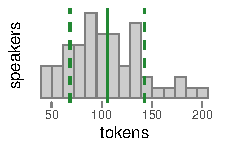
\includegraphics[width = 1.5in]{Figures/BAT/BAT_tiny.pdf}} and the average number of tokens per generation per sex was about 713. In this dataset, \bat varies considerably across ages and sexes and the patterns that are found in this sample reflect similar patterns described in other areas in the West.

\begin{figure*}[tb!]
	\centering
	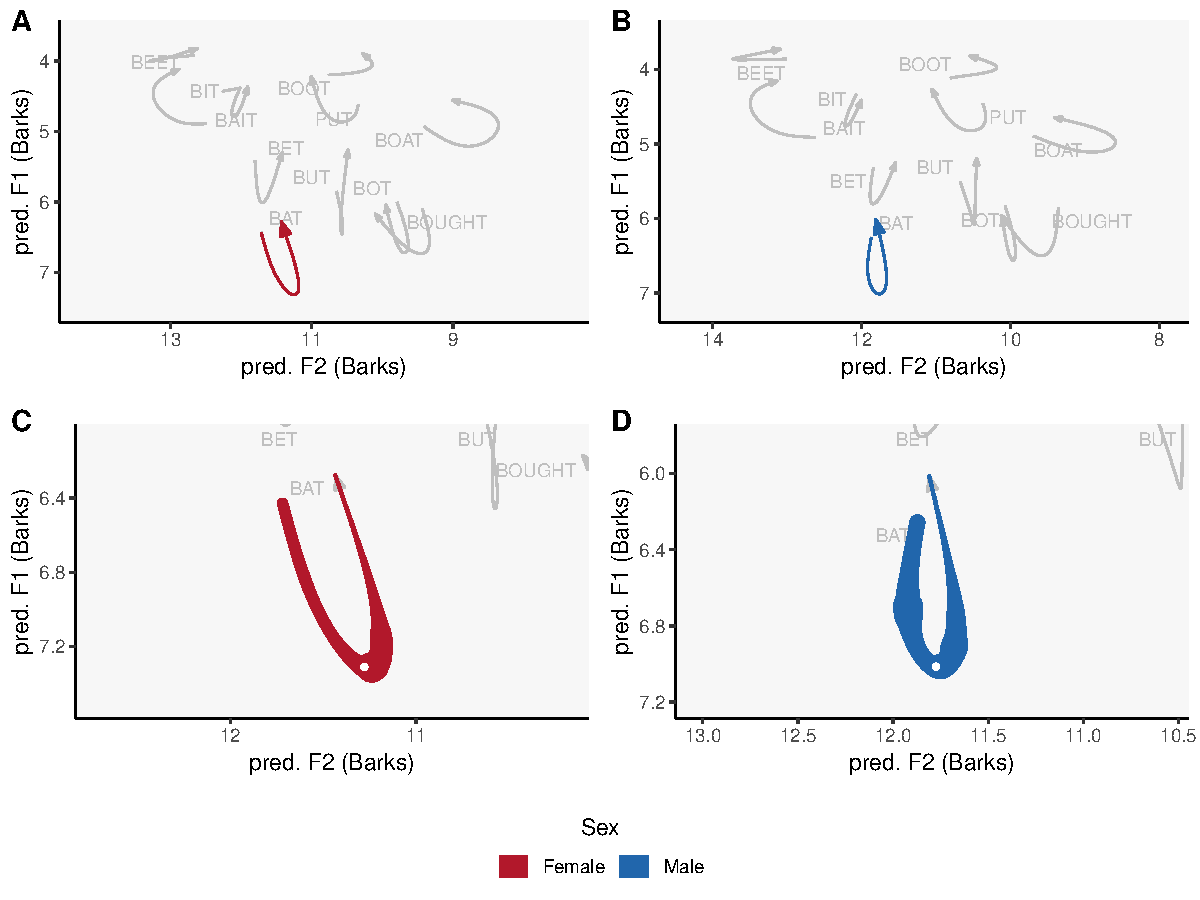
\includegraphics[width = 6.5in]{Figures/BAT/BAT_four_panel_plot_summarized.pdf}
	\caption[Predicted formant measurements for \bat by sex.]{Predicted formant measurements for \bat by sex with women on the left and men on the right. Predicted values are averaged across all generations.}
	\label{fig:BAT_four_panel_summarized}
\end{figure*}

Figure~\ref{fig:BAT_four_panel_summarized} shows the effect that sex had on the \bat vowel in a four-panel plot.\footnote{For details on how to interpret this and subsequent plots, see \S\ref{sec:visualizing_gamms}} It is immediately clear that this vowel is not monophthongal but that there is some vowel-inherent spectral change. Specifically, the vowel exhibits something like a V or U shape: it gets lower during the first half of its duration before raising again during the second half. As seen in panels A and B, there is a fair amount of movement in \bat; the trajectory length was 2.002 Barks.\footnote{This is calculated by extracting predicted values for \bat at 501 time points and getting the sum of the Euclidean distances in the Bark F1-F2 space from each point to the next consecutive point. Basically, I apply the methods described by \citet{fox_jacewicz_2009}, only except taking the sum of 4 segments, I take the sum of 500 segments simply because I have the ability to extract that many predicted values from the GAMMs.} In fact, the trajectory length of \bat was the longest out of any allophone of any of the front lax vowels in this sample. However, at no point does \bat overlap with any other vowel, so \bat is contained in its own portion of the vowel space. There appears to be a clear target for this vowel for both F1 and F2 that is approximately at the halfway point of its duration. By ``target'' I mean that the visual shape of this trajectory achieves its lowest point at approximately the midpoint of its duration. Based on these trajectory shape, the vowel is a triphthong, with a low front nucleus and raised offglides: [\textipa{\textsubarch{\|'\ae}\ae\textsubarch{\|'\ae}}]. There is no immediately obvious difference between the sexes in Figure~\ref{fig:BAT_four_panel_summarized}, suggesting that the way this vowel is realized is approximately the same for both men and women.

\begin{figure*}[tb!]
	\centering
	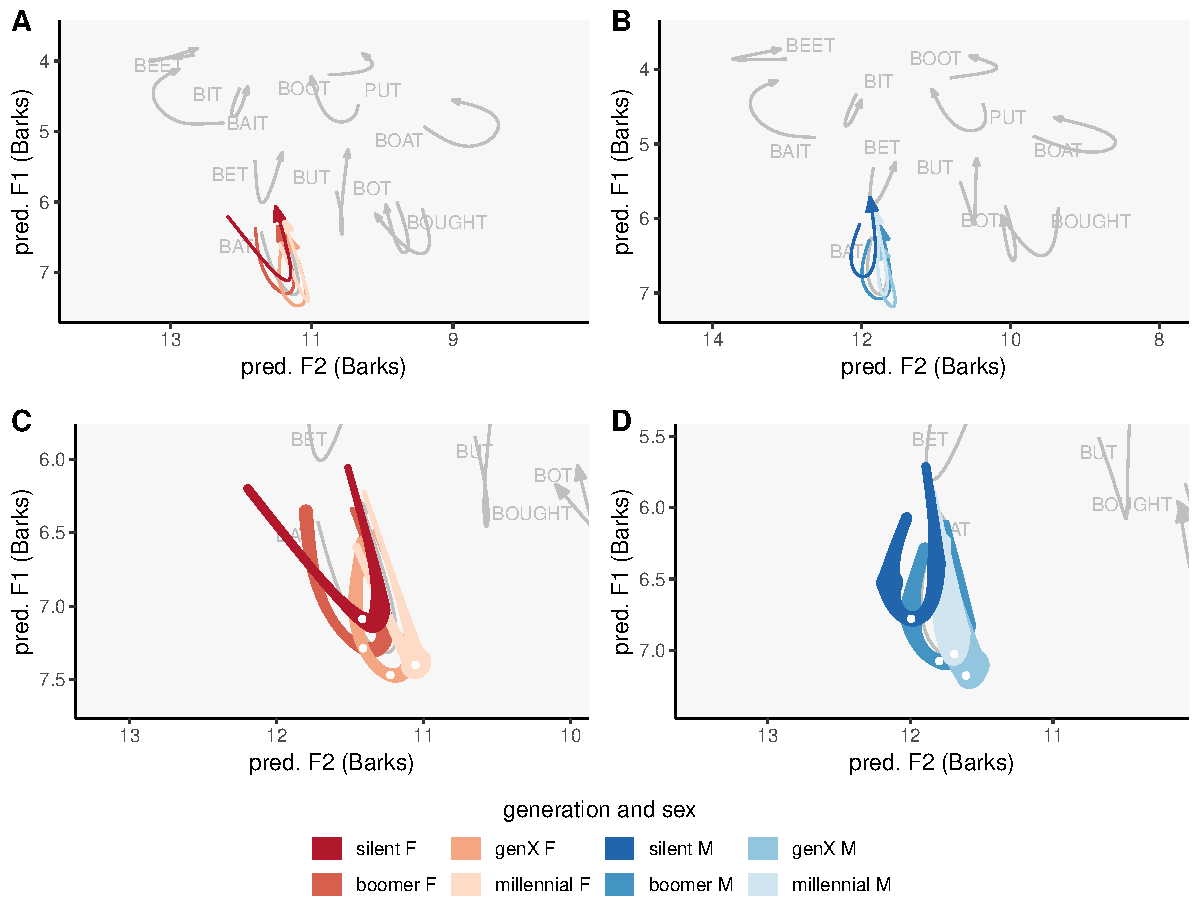
\includegraphics[width = 6.5in]{Figures/BAT/BAT_four_panel_plot.pdf}
	\caption[Predicted formant measurements for \bat by sex and generation.]{Predicted formant measurements for \bat by sex and generation. Women are on the left and men on the right. Darker shades represent older generations.}
	\label{fig:BAT_four_panel}
\end{figure*}

When the data is split up by the four generations in this sample and by sex, the differences between the sexes become more defined. Figure~\ref{fig:BAT_four_panel} shows the predicted trajectories for \bat for each combination of generation and sex from the GAMM. Beginning with the women, we see that the target of \bat, which happens to occur near the midpoint of the vowel gradually lowers and then retracts. Difference smooths (Appendix~\ref{appendix:difference_smooths}, Figure~\ref{fig:bat_diff_smooths_gen}, Panels A--B, M--N, U--V) suggest that the change between successive generations of women was relatively small, but when comparing nonconsecutive generations the difference reaches statistical significance (\ref{fig:bat_diff_smooths_gen}, E--F, I--J, Q--R). For instance, compared to the Silent generation, Boomer women had no significant change in the height of \bat (\ref{fig:bat_diff_smooths_gen}A), and compared to the Boomers, neither did the Gen X women (\ref{fig:bat_diff_smooths_gen}M); but when compared to the Silent women, Gen X women had a significantly higher F1 (corresponding to a lower vowel) along the majority of its trajectory (\ref{fig:bat_diff_smooths_gen}E). Retraction of \bat occurred primarily in the first half of the vowel's trajectory and also in the later three generations, with each generation shifting a small portion of the beginning half to a more retracted portion of the vowel space. This uneven retraction within the vowel resulted in a change in shape from a V to a Bounce. In summary, we see that the changes in the women's realizations of \bat include lowering and retraction, primarily in the first half of the trajectory.

Turning to the right panels in Figure~\ref{fig:BAT_four_panel}, we can begin to analyze the men's realizations. Some of the patterns are shared with the women's realizations of \bat. For example, the Gen X men had a significantly lower realization of \bat than the Silent men along the entire course of its trajectory. However, difference smooths suggest that there are further changes that were not found in the women's data. For one, this pattern of lowering \bat was statistically significant between the oldest two generations, but only in the second half of the trajectory (\ref{fig:bat_diff_smooths_gen}C). There is also a pattern of retraction, though it is only large enough to reach statistical significance when comparing the Silent Generation to the two younger groups and is centered around the 25\% point in the duration of the vowel (\ref{fig:bat_diff_smooths_gen}H,L). So for the men, we find that the bulk of the changes occurred first in last half of \bat's trajectory where the younger generations used lowered offglides and then in the first half of the trajectory where younger generations used a fronter nucleus. It is noteworthy that all of these changes were not centered around the midpoint of the vowel, but it is indeed the trajectories of the vowel that are undergoing change. Like the women, we see a change from a V- or U-shaped curve to a Bounce in apparent time during the time that the midpoints shift.

Figure~\ref{fig:BAT_four_panel} therefore suggests a pattern of gradual lowering and retraction, primarily in the first half of the vowel's trajectory, over the course of the four generations in this sample. This pattern is noticeably different from what was found in California, where the primary direction of change is in F2 \citep{donofrio_etal_2019}. Here, the differences between successive generations were generally small and were only noticeably when comparing speakers to their grandparents' or grandchildren's generation. It appears then that the lowering and retraction of \bat is active and has been steadily advancing for at least four generations in Cowlitz County.

\begin{figure*}[p]
	\centering
	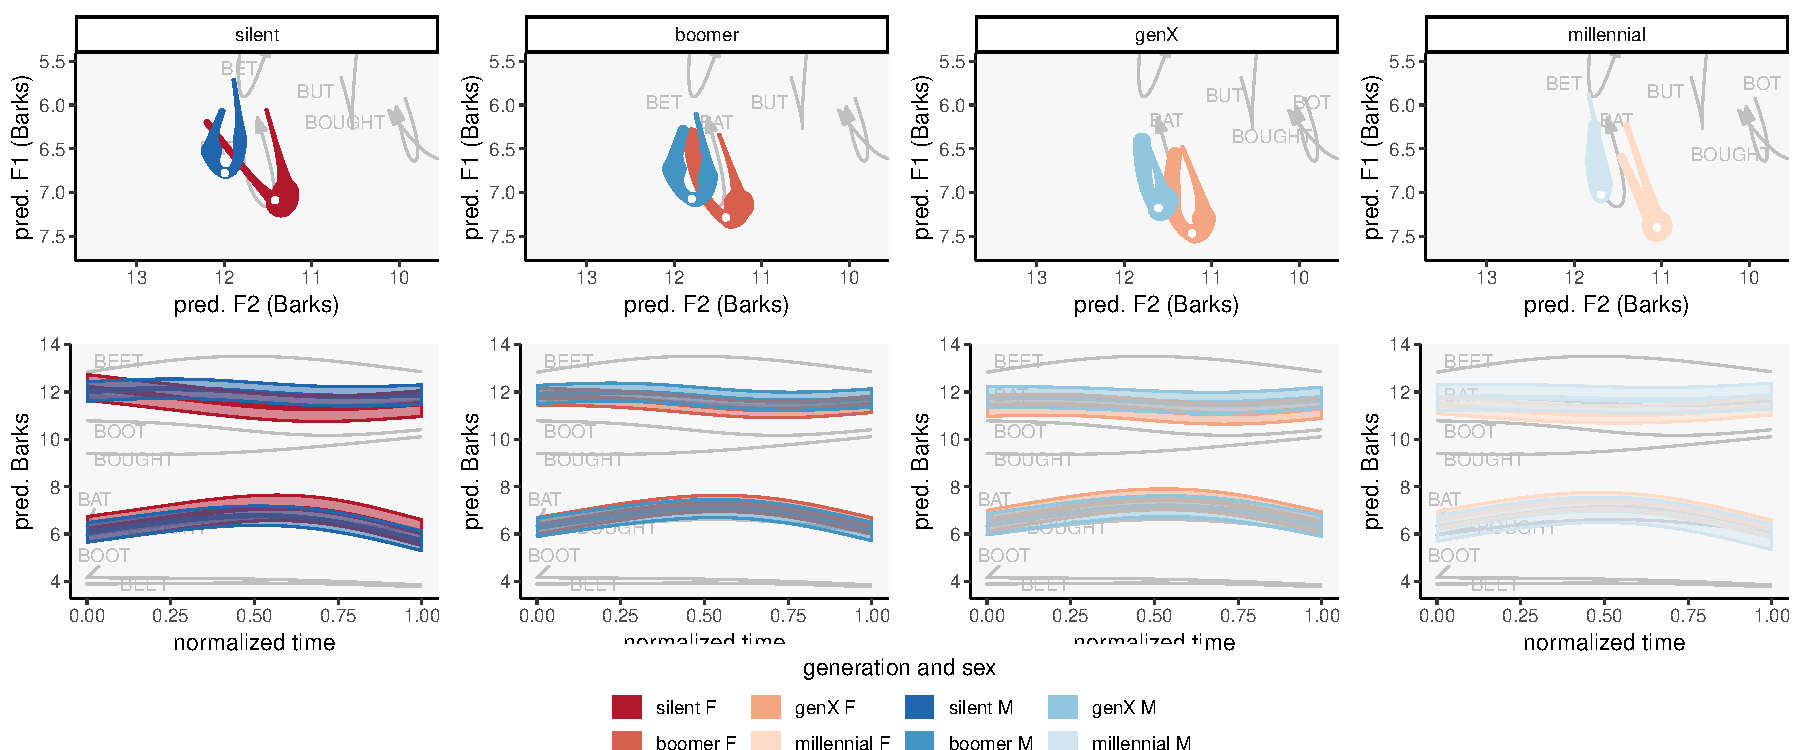
\includegraphics[angle = 90, origin = c, height = 6in]{Figures/BAT/BAT_sex_panel_plot_wide.pdf}
	\caption[Predicted formant measurements for \bat by generation.]{Predicted formant measurements for \bat by generation.}
	\label{fig:BAT_sex_panel_plot_wide}
\end{figure*}

As an alternative view of the data, Figure~\ref{fig:BAT_sex_panel_plot_wide} shows the same predicted trajectory data but split up by generation rather than by sex. Because the data are normalized, an apples-to-apples comparison can be made between the sexes within each generation. This visualization makes it apparent that there are differences between the sexes in all generations and that these differences are roughly consistent in apparent time: women use a more lowered and retracted variant of \bat than men in their generation. Difference smooths between these pairs of predicted trajectories (Appendix~\ref{appendix:difference_smooths}, Figure~\ref{fig:bat_diff_smooths_sex_gen}) suggest that women lead this change both in F1 and F2 for all four generations, reaching statistical significance in most pairs. Among the Silent, the difference is significant during the last half of the F1 trajectory and in all but the first 20\% of F2 (\ref{fig:bat_diff_smooths_sex_gen}A,B). Among the Boomers, the difference is slightly smaller, and is only significant in F2 (\ref{fig:bat_diff_smooths_sex_gen}C,D). For Gen X, the difference again only reached statistical significance for F2 (\ref{fig:bat_diff_smooths_sex_gen}E,F) suggesting that perhaps the men caught up with the women at least in the height dimension. But for the Millennials, the women's trajectory is significant different from the men's for the entire duration of the vowel for both F1 and F2 (\ref{fig:bat_diff_smooths_sex_gen}G,H). A trend in these difference smooths is that the significance is primarily found in the latter portion of the vowel's trajectory, suggesting that what makes men's and women's realizations of \bat is the realization of the entire offglide.

Another pattern is the gradual flattening of the F2 formant curve over time. The Silent women had a clear V-shaped trajectory and the men had something between a V and a U. However, over the course of the four generations, these curves become narrower so that the Millennials of both sexes have Bounce-shaped curves. Though the men lag behind the women in the position of their vowel, the men keep up with the women in its shape.

Taking Figures~\ref{fig:BAT_four_panel} and \ref{fig:BAT_sex_panel_plot_wide} together, we see a clear case of language change in apparent time, with women in the lead. The differences across generations, which were primarily in the first half of the trajectory, were relatively small and did not often reach statistical significance between consecutive generations, but they add up to show a modest amount of change over the 67 years of apparent time data in this sample. Women are consistently ahead of men in the position of the vowels, especially in the second half of the trajectories. Putting these descriptions together, we see a continuous and relatively constant rate of change, but the complex nature of this shift, with different parts of the trajectory changing at different rates, highlights the need for analyzing trajectories rather than midpoints alone.


% ---------------------------------------------------------------------------------
% ------------------------------    BET    ----------------------------------------
% ---------------------------------------------------------------------------------
\section{\bet}
\label{BET}

In this sample, there were 7,943 tokens of \bet coming from 771 unique words. The most frequent of these words were \textit{said}, \textit{yes}, \textit{everything}, \textit{never}, \textit{every}, \textit{ever}, \textit{everybody}, \textit{whatever}, \textit{guess}, and \textit{together}. Because the GAMM included a random intercept for word, it adjusts for the fact that many of these words have the vowel followed by /\textipa{v}/. Each speaker produced an average of 143 tokens of \bet\footnote{Speakers ranged from 56 to 404 tokens with a standard deviation of 59.9: 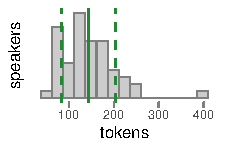
\includegraphics[width = 1.5in]{Figures/BET/BET_tiny.pdf}} resulting in approximately 997 per generation per sex.

\begin{figure*}[tb!]
	\centering
	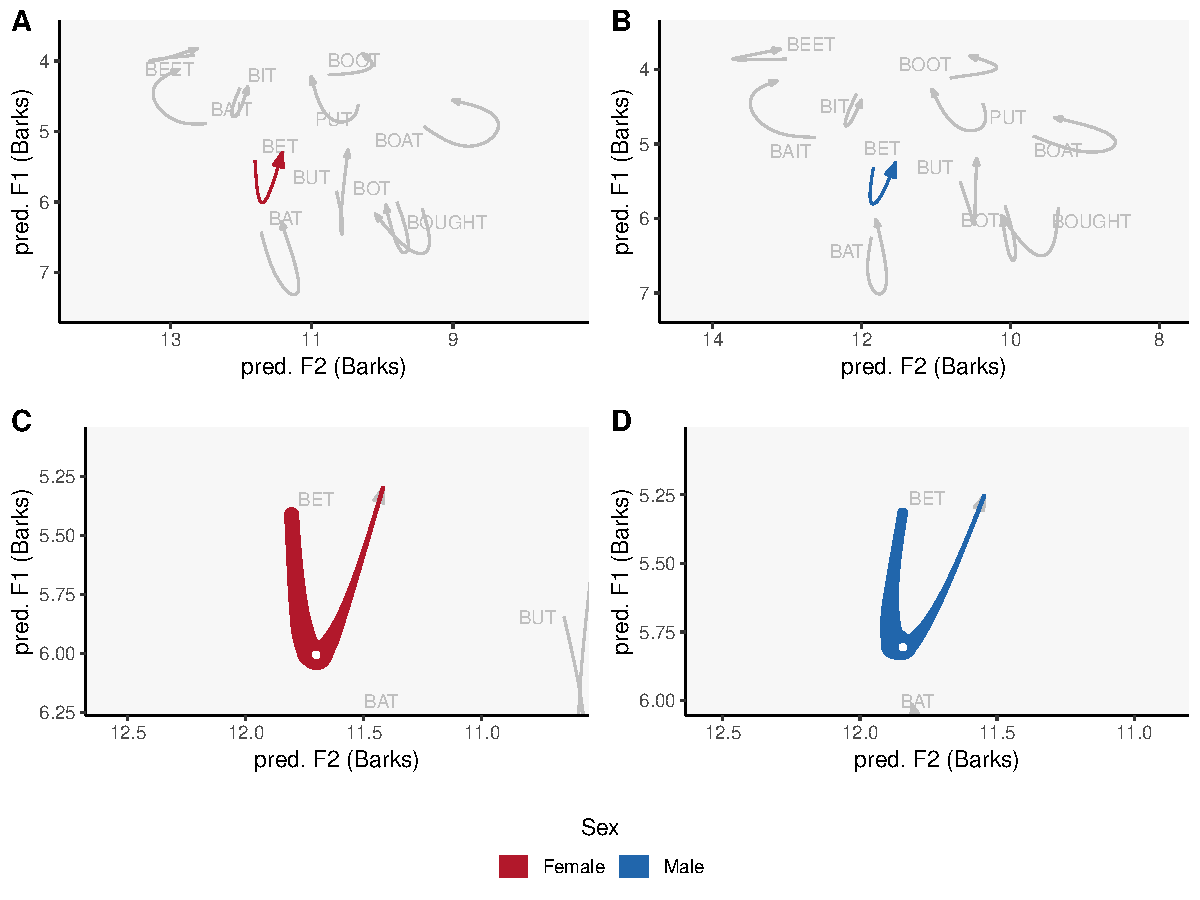
\includegraphics[width = 6.5in]{Figures/BET/BET_four_panel_plot_summarized.pdf}
	\caption[Predicted formant measurements for \bet by sex.]{Predicted formant measurements for \bet by sex with women on the left and men on the right. Predicted values are averaged across all generations.}
	\label{fig:BET_four_panel_summarized}
\end{figure*}

Figure~\ref{fig:BET_four_panel_summarized} offers a first look at how \bet is realized in this sample. Regarding its relative position in the vowel space, \bet shares approximately the same F2 space as \bat but is equal in height with \strut and midway between the low back vowels and \goat. Compared to \bat, the shape of the trajectory of \bet is similar with an approximately V-shaped curve that starts fronter, reaches a clear target near the midpoint, and then ends more centralized. However, compared to \bat, panels A and B of Figure~\ref{fig:BET_four_panel_summarized} show that the overall amount of movement that \bet undergoes is relatively small. In fact, while the predicted trajectory length of \bat was 2.002 Barks, \bet was only 1.264 Barks. Clearly \bet is more monophthongal than \bat in this sample, so it is difficult to say whether the vowel as a triphthong analogous to \bat [\textipa{\textsubarch{\|'E}E\textsubarch{\|'E}}] or if it is a pure monopthong [\textipa{E}]. Comparing panels C and D, there are no obvious differences between the sexes when all generations are pooled together.

\begin{figure*}[tb!]
	\centering
	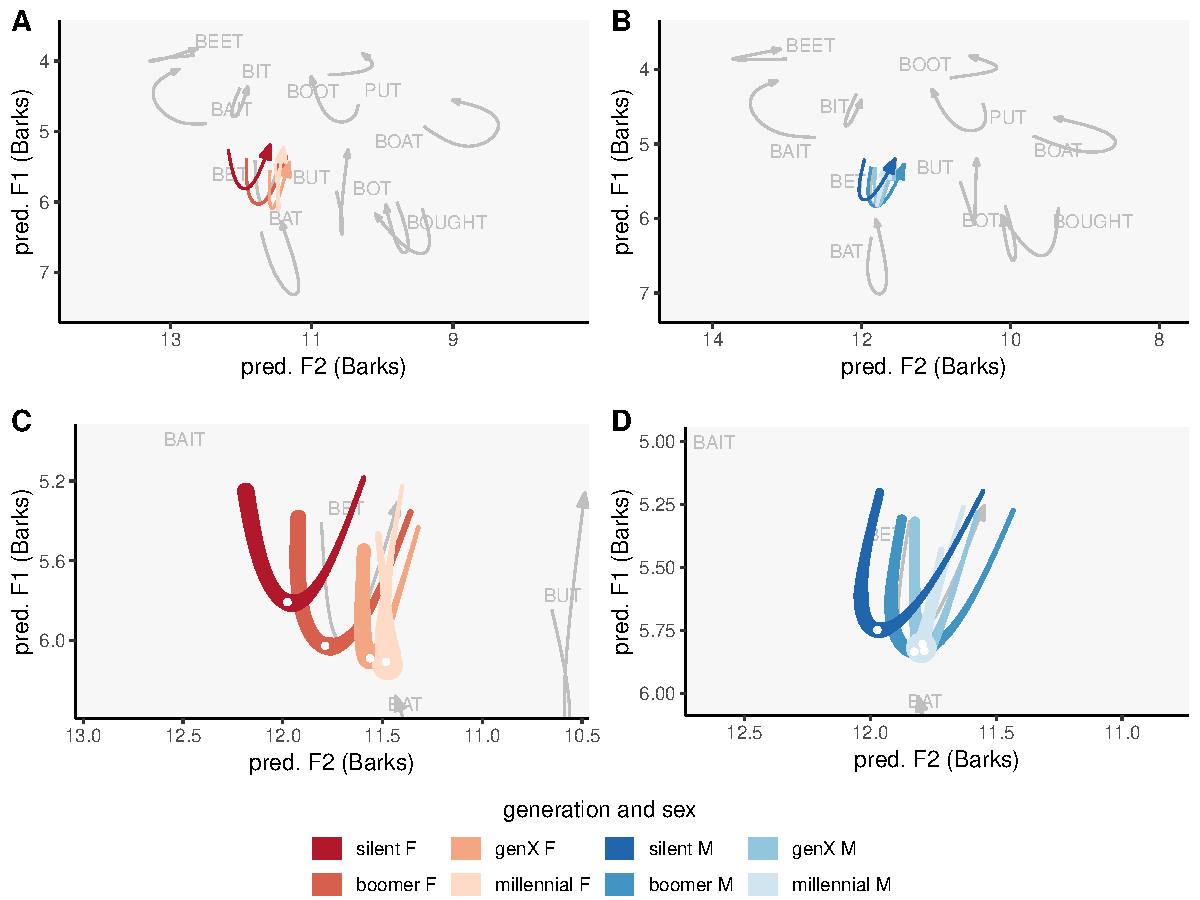
\includegraphics[width = 6.5in]{Figures/BET/BET_four_panel_plot.pdf}
	\caption[Predicted formant measurements for \bet by sex and generation.]{Predicted formant measurements for \bet by sex and generation. Women are on the left and men on the right. Darker shades represent older generations.}
	\label{fig:BET_four_panel}
\end{figure*}

Splitting the data by generation, as in Figure~\ref{fig:BET_four_panel}, offers a more nuanced view at how \bet changes in apparent time. Beginning with the women on the left, panel C shows that \bet simultaneously lowers, retracts, and changes shape in apparent time. Like \bat, the change in the height of \bet is relatively small from one generation to the next (Appendix~\ref{appendix:difference_smooths}, Figure~\ref{fig:bet_diff_smooths_gen}A--B, M, U--V), but when skipping generations, difference smooths suggest that the lowering is statistically significant (\ref{fig:bet_diff_smooths_gen}E--F,I--J,R), but (again) only in the first half of the trajectory. The direction of change was greater along the F2 dimension and the first half of the trajectory was backed more than the offset. The largest jump in \bet retraction was between the Boomers and Gen X and did reach statistical significance, at least in the first half of the vowel's duration (\ref{fig:bet_diff_smooths_gen}N). Difference smooths suggest that the younger two generations had a significantly more retracted \bet than the Silent Generation for essentially the entire duration of the vowel (\ref{fig:bet_diff_smooths_gen}F,J); this is supported in panel C of Figure~\ref{fig:BET_four_panel} where the onset of the Millennial women's \bet had a lower F2 than even the offset of that of the Silent women. The result of the onset shifting more than the offset is a change in trajectory shape in apparent time: the older generations have a more U-shaped curve where F2 gradually lowers over the course of the vowel's duration while the younger generations' \bet is pointier, culminating in Millennials' realizations with hardly any change in F2: a prototypical Bounce. While the entire vowel is lowering and retracting, it is doing so at an uneven rate and it appears that the onset has ``caught up'' to the offset. Speculatively, if this trend continues, future generations of Washington women may reverse the shape of \bet entirely, such that it starts as a central vowel and glides towards the front.

In stark contrast to the women's intriguing pattern, the men show relatively little change in \bet's position in apparent time. Superficially, panel D shows that the men exhibit a similar pattern of lowering, retraction, and reduction in the range of F2 that the vowel crosses through, but the amount of change from one generation to the next is small. In fact, difference smooths show no statistical significance in either F1 or F2 between any generation of men, except for a small portion near the onset that was significantly more retracted for the Millennials and Gen X than the Silent men, but this may not be found in other samples (\ref{fig:bet_diff_smooths_gen}H,L). In other words, \bet is relatively stable in this sample of Cowlitz County men and does not show change in apparent time.

\begin{figure*}[p]
	\centering
	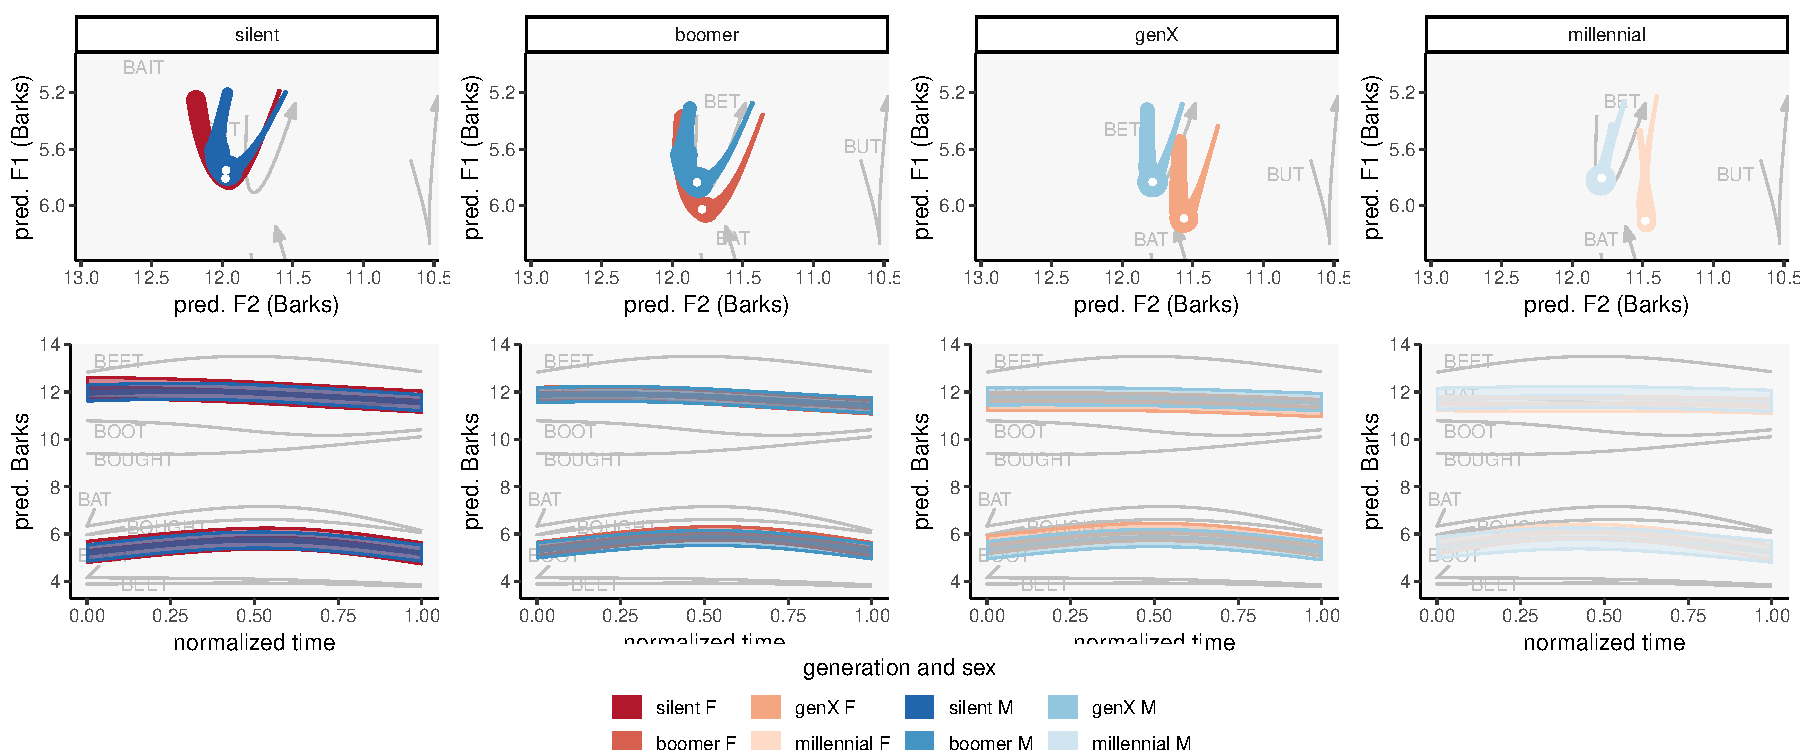
\includegraphics[angle = 90, origin = c, height = 6in]{Figures/BET/BET_sex_panel_plot_wide.pdf}
	\caption[Predicted formant measurements for \bet by generation.]{Predicted formant measurements for \bet by generation.}
	\label{fig:BET_sex_panel_plot_wide}
\end{figure*}

The question that remains then is how the women compare to the men in their relative positioning. Is it the case that the women are shifting away from the men or did the men start with a more centralized vowel and the women are shifting towards them? Figure~\ref{fig:BET_sex_panel_plot_wide} provides evidence for the former. The leftmost panel of Figure~\ref{fig:BET_sex_panel_plot_wide} plots the women and men in the Silent Generation and shows that they have very similar realizations of \bet, both in position and shape of the curve; difference smooths suggest no difference between the sexes. We can therefore conclude that there the oldest generation of speakers in this sample realized \bet the same way. However, Figure~\ref{fig:BET_sex_panel_plot_wide} shows that as the speakers get younger, the sexes diverge. Among the Boomers and Gen X, the difference is primarily in height, and difference smooths (\ref{fig:bet_diff_smooths_sex_gen}C,E) suggest a statistically significant difference in F1 just in the middle 15\% and third of the vowel, respectively. Between the Millennials, the difference in height expands to the middle 50\% of the vowel in F1 and the middle two-thirds for F2. In other words, difference smooths support what is visually apparent in Figure~\ref{fig:BET_sex_panel_plot_wide}: men and women's realizations of \bet gradually separate with each successive generation. And the fact that the oldest generation started off with no difference between them suggests that there was no change at that time and that this sample captures the beginning of this vowel shift change in Cowlitz County.

In addition to their separation in apparent time, GAMMs provide an additional and intriguing insight when looking at \bet: the shape of the vowel trajectories was quite similar between the sexes across all generations. This is not a consequence of the model: recall that the GAMM fit each combination of sex and generation as independent factors, and though a human analyst knows that female Millennials have the same age range as male Millennials, the model was not ``aware'' of this fact. This makes it all the more surprising that each generation's vowel trajectories were similar in shape. So far in this analysis of \bet, I have suggested that language change is happening among the women but not the men. If only the midpoints were analyzed, this may be a reasonable conclusion. But while the men's realizations are relatively stable in the vowel space, their trajectories are in sync with the changes that the women are doing: a gradual shift from a U to a Bounce. These similarities across generations are a curious case of language change where men are keeping up with the women but only in one aspect of the shift. This also justifies the use of GAMMs because this kind of effect could not easily be detected if only one measurement were taken per vowel.

Summarizing the findings for \bet, this section has shown changes in apparent time that are conditioned by the sex of the speaker. Women are lowering, retracting, and changing the shape of \bet while men are simply changing its shape while remaining more or less in the same relative position in the vowel space. Specifically, the trajectory is changing such that the first half of the vowel is shifting faster than the second half, resulting in a change from a U-shape to a Bounce in the F1-F2 space. Finally, the Boomers initiated this shift since the differences between the sexes was negligible in the Silent generation.



% ---------------------------------------------------------------------------------
% ------------------------------    BIT    ----------------------------------------
% ---------------------------------------------------------------------------------

\section{\bit}
\label{BIT}


% I'll need to rerun the models after removing getting and different, maybe.
The final vowel to be analyzed in this chapter is \bit. In this sample, there were 8,231 tokens of \bit coming from 736 unique words. The most frequent of these words were \textit{different}, \textit{little}, \textit{kids}, \textit{pretty}, \textit{lived}, \textit{bit}, \textit{six}, \textit{live}, and \textit{river}. Each speaker produced an average of 152 tokens of \bit\footnote{Speakers ranged from 59 to 323 tokens with a standard deviation of 49.7: 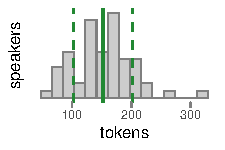
\includegraphics[width = 1.5in]{Figures/BIT/BIT_tiny.pdf}} meaning there were approximately 1029 per generation per sex.

\begin{figure*}[tb!]
	\centering
	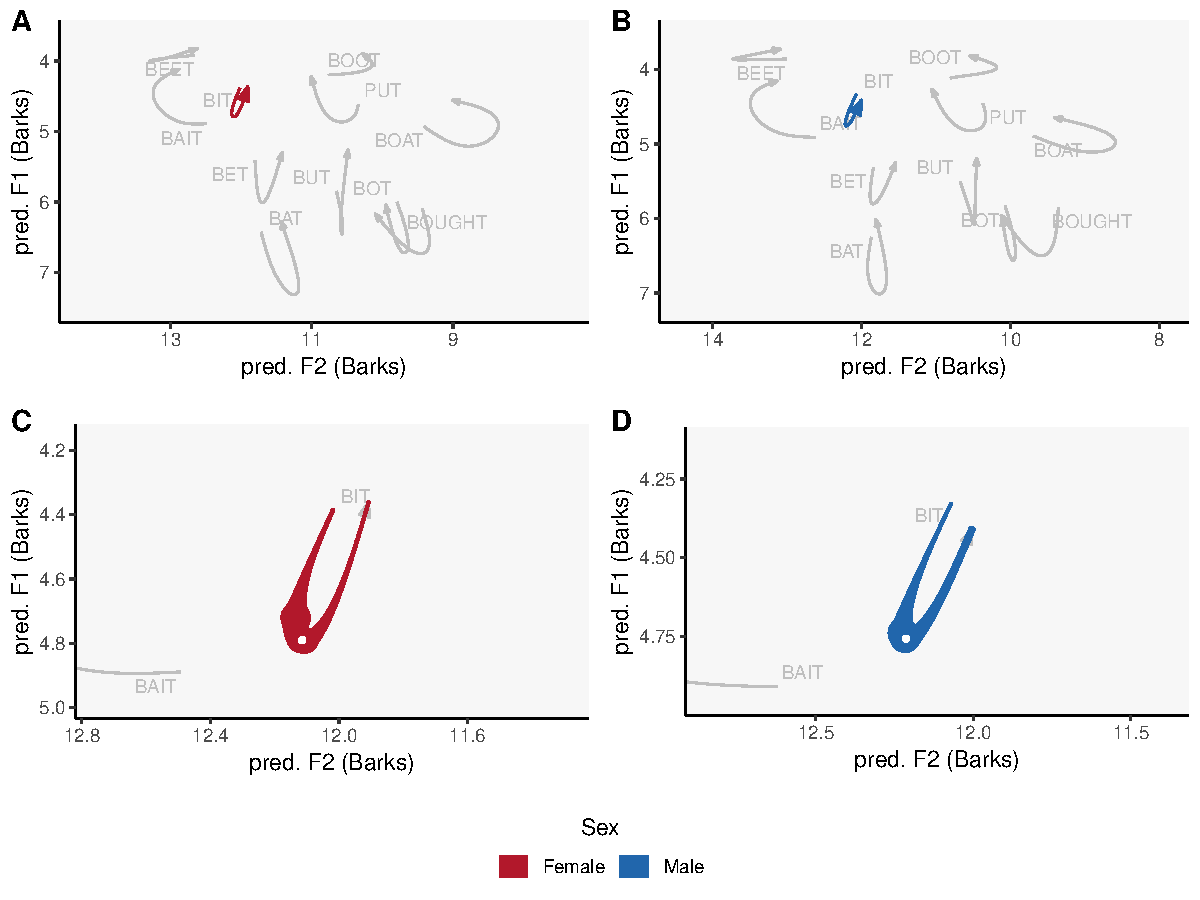
\includegraphics[width = 6.5in]{Figures/BIT/BIT_four_panel_plot_summarized.pdf}
	\caption[Predicted formant measurements for \bit by sex.]{Predicted formant measurements for \bit by sex with women on the left and men on the right. Predicted values are averaged across all generations.}
	\label{fig:BIT_four_panel_summarized}
\end{figure*}

Figure~\ref{fig:BIT_four_panel_summarized} offers a preliminary analysis of \bit in this sample of Cowlitz County speakers. Its relative position compared to other vowels is that is about the same height as \face and \strut and slightly fronter than \bet and \bat. Like \bat and \bet, the \bit vowel takes on a U-shaped curve, starting higher and fronter, dipping towards a target near the midpoint, and ending at a point about as high as the onset but more centralized. However, it is the least dynamic vowel among the the front lax vowels with an average trajectory length of 0.903, which is slightly less than half the length of \bat. In this case, I am more comfortable describing the vowel as a pure monopthong [\textipa{I}] than as a triphthong like \bat and possibly \bet. Like the other vowels, when the data is summarized for all speakers of the same sex as in Figure~\ref{fig:BIT_four_panel_summarized}, there are no obvious differences between how men and women realize this vowel.

\begin{figure*}[tb!]
	\centering
	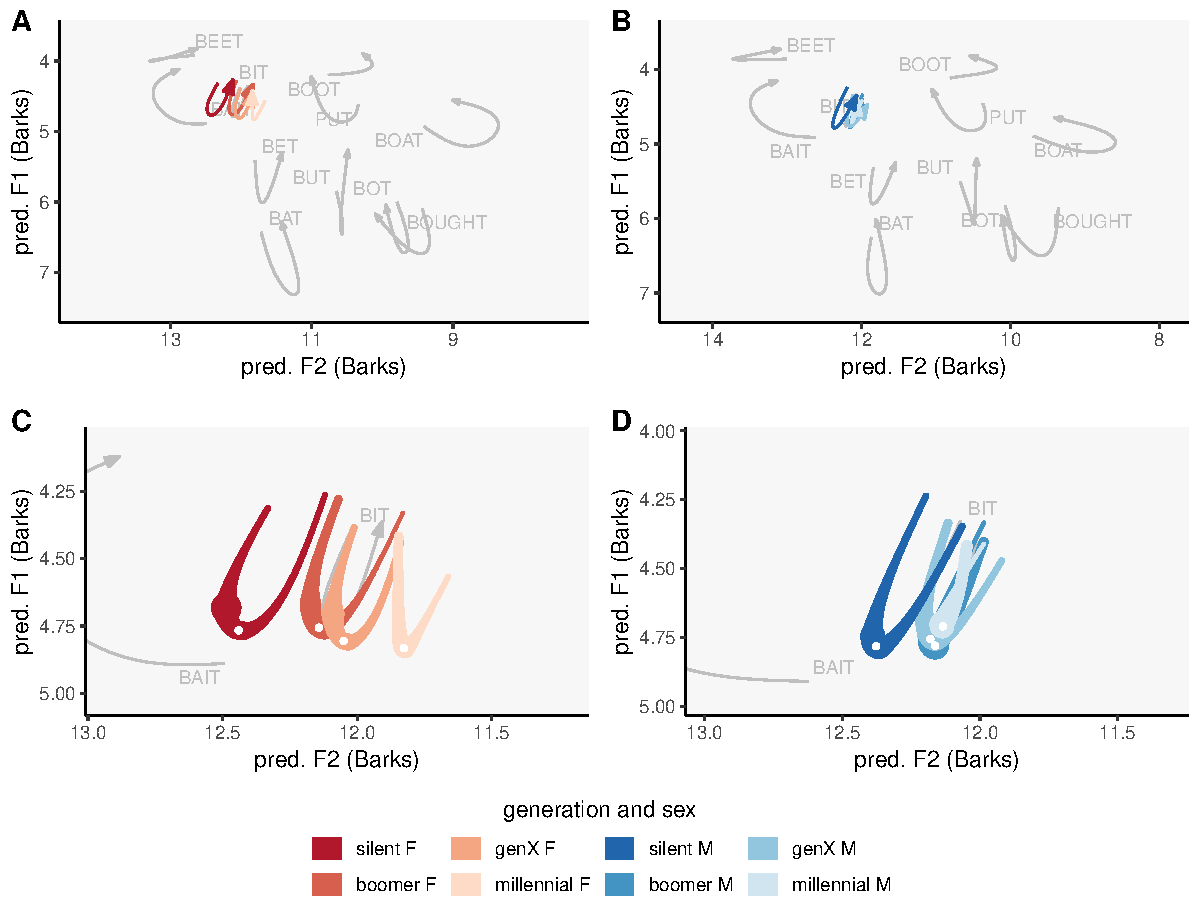
\includegraphics[width = 6.5in]{Figures/BIT/BIT_four_panel_plot.pdf}
	\caption[Predicted formant measurements for \bit by sex and generation.]{Predicted formant measurements for \bit by sex and generation. Women are on the left and men on the right. Darker shades represent older generations.}
	\label{fig:BIT_four_panel}
\end{figure*}

But, when the data is split up by sex and generation, then patterns in apparent time emerge. Panels A and C of Figure~\ref{fig:BIT_four_panel} shows a pattern of \bit retraction in apparent time among the Cowlitz County women in this sample. The women in the Silent Generation use the most fronted variant of \bit, but with each generation the vowel becomes incrementally more retracted. The amount of change in the vowel space is relatively small, but difference smooths suggest that much of this retraction is statistically significant (\ref{fig:bit_diff_smooths_gen}B,F,J,R,V). From the Silent to the Boomers, the difference was significant along the entire trajectory of the vowel (\ref{fig:bit_diff_smooths_gen}B), which is supported by the lack of overlap between the two curves in Figure~\ref{fig:BIT_four_panel}. Between the Boomers and Gen X, the difference was not significant at all (\ref{fig:bit_diff_smooths_gen}N). But between Gen X and the Millennials, the first half of the trajectory was significantly more retracted (\ref{fig:bit_diff_smooths_gen}V). This on-again-off-again pattern of retraction may be indicative of the end of one shift and the beginning of a new phase of \bit retraction. Regarding vowel height, there was very little evidence of \bit lowering in this sample (\ref{fig:bit_diff_smooths_gen}A,E,I,M,Q,U)

Moving on to panels B and D of Figure~\ref{fig:BIT_four_panel}, we see a pattern reminiscent of what was found with \bet: relatively little change. While the women are undergoing a gradual but robust process of \bit retraction, the men do not appear to be following suit. There is some degree of retraction between the oldest two generations of men, and the difference smooths suggest that the shift in the first half of the trajectory was statistically significant (\ref{fig:bit_diff_smooths_gen}D). But otherwise, \bit is remarkably stable among Cowlitz County men, at least in the vowel's position in the vowel space.

\begin{figure*}[p]
	\centering
	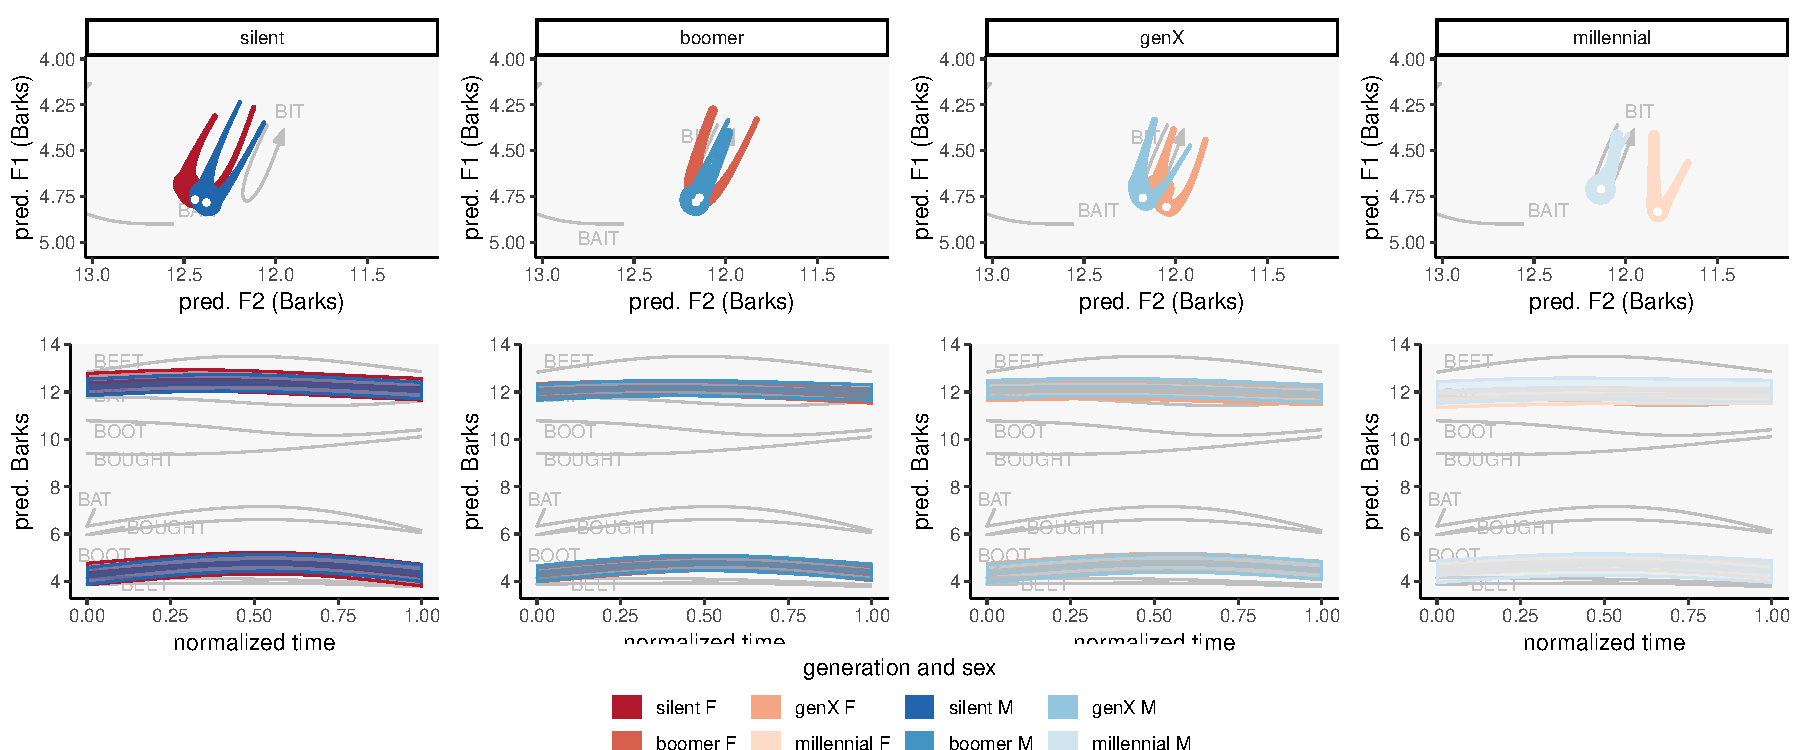
\includegraphics[angle = 90, origin = c, height = 6in]{Figures/BIT/BIT_sex_panel_plot_wide.pdf}
	\caption[Predicted formant measurements for \bit by generation.]{Predicted formant measurements for \bit by generation.}
	\label{fig:BIT_sex_panel_plot_wide}
\end{figure*}

A within-generation comparison of men and women, as in Figure~\ref{fig:BIT_sex_panel_plot_wide}, illuminates additional insight into how \bit is realized in this community. Basically, there is little difference between the men and women within most generations. Difference smooths suggest that the vowel trajectories of these two sexes were not statistically different in either F1 or F2 (\ref{fig:bit_diff_smooths_sex_gen}A--G). The exception to this are the Millennials, and women's realizations were significantly more retracted than the men's for the first two thirds of the trajectory (\ref{fig:bit_diff_smooths_sex_gen}H). So while the women appear to be shifting more in relation to the men, because the amount of shifting was so small, the differences between the sexes is not apparent until the youngest generation.

In addition to the change in position, there are some additional changes in the trajectory shape. Among the women, there is a sudden change from a U in the older three generations to a V in the Millennials, which may reinforce the hypothesis that a new shift is beginning among that youngest generation of women. Among the men, it oscillates between a narrow U and a Bounce. In general for \bit though, it is possible that because this vowel is so monophthongal that the trajectory itself is not particularly important.

Summarizing the findings for \bit, overall it was the least dynamic vowel and undergoes the smallest amount of change. Women are participating in a pattern of retraction, and \bit is gradually becoming a more centralized vowel, though the amount of change in the vowel space is relatively small. Men retracted somewhat, but for the past three generations the vowel is stable.

\section{Discussion}
\label{sec:preobstruent_discussion}

In the previous sections, I presented the results of generalized additive mixed-effects models on the elsewhere allophones of \trap, \dress, and \kit. This section summarizes these findings, proposes a hybrid of chain shifting and parallel shifting in this community, and links these results with speech patterns found in other communities in the West. I then justify the use of GAMMs by discussing the trajectory-related findings in this chapter.

\subsection{Summary of findings}
\label{bat_bet_bit_summary}

The previous sections have shown that each vowel underwent a variety of changes over time. First, The \bat vowel slowly lowered and retracted in apparent time, with the primary direction of change being in vowel height. In Cowlitz County, this change is being led by the women. In particular the first half of the vowel trajectory shifts more than the last half, meaning that the trajectory shape changes from a V to a Bounce. Compared to the other front lax vowels, \bat was the most dynamic.

In women's speech, the \bet vowel lowered and retracted about the same amount while the men's variants of \bet were in approximately the same position in the vowel space. For both sexes, the shape of \bet gradually shifted from a U also to a Bounce as a result of the first half advancing at a faster rate in apparent time than the second half. The trajectory length of \bet was shorter than \bat, making it a more monophthongal vowel.

\bit undergoes the least amount of change. There was very little change in the vowel height and the retraction found in the women's speech was statistically significant but relatively small. There was no shifting in the men's speech at all. The trajectory shape was inconsistent across generations and devoid of clear patterning, other than perhaps a switch from a U to a V among the women. The trajectory length of \bit was a little less than half that of \bat, making it the least dynamic of the front lax vowels.

What do these findings say about the structural relationship of these three vowels in Cowlitz County, and how does this Washington community fit in with neighboring cities?

\subsection{Chain shift, parallel shift, or both?}
\label{sec:what_kind_of_shift}

In \S\ref{sec:structure_of_elsewhere_shift}, I describe how there is inconsistency across regions in how the vowels are shifting. In particular, \citet{boberg_2005} explains that this has implications for whether this movement is a chain shift or a parallel shift. If the vowels undergo a rotation in the vowel space, meaning \bet and \bit lower as \bat retracts and lowers, then there is evidence for a chain shift. However, if the vowels are retracting only, then this may be a parallel shift.

\begin{figure}[tb!]
    \centering
    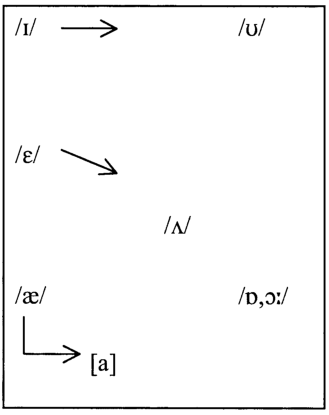
\includegraphics[width = 0.5\textwidth]{Figures/other_figures/montreal_shift.pdf}
    \caption[The Elsewhere Shift in Montreal and Cowlitz County.]{The Elsewhere Shift in Montreal and Cowlitz County. From \citet[149]{boberg_2005}.}
    \label{fig:montreal_shift}
\end{figure}

The patterns found in Cowlitz County are somewhat of a combination of these two idealized scenarios. \bat is lowering with a small amount of retraction, \bet is both lowering and retracting, and \bit is retracting only; all three vowels are moving in different directions. Because \bit is not lowering, a chain shift model---at least one that involves \bit---is not supported. However, because all three vowels do retract to some degree, Cowlitz County vowels very closely match the parallel shift that \citet{boberg_2005} describes in Montreal (Figure~\ref{fig:montreal_shift}). So which is it, a chain shift, a parallel shift, or both?

Perhaps the front lax vowels are not all structurally related; specifically it may be the case that \bet and \bat are chain shifting while \bit is moving independently. Because \bit, \bet, and \bat form a natural class of front lax vowels in English, an elegant description would be that they all move as a unit, but this data suggest that only \bet and \bat are lowering. The \textit{Atlas of North American English} famously includes only \bet lowering and \bat retraction in its definition of the Canadian Shift (in addition to \lot retraction; \citealt[219]{labov_ash_boberg_2006_anae}), so at least in their data \bit was not related to the other two vowels.\footnote{\citet{donofrio_etal_2019} also find that \bat and \bet lower and retract but not \bit, so it's not out of the question that \bit be left out in this analysis.} It may be the case that the Elsewhere Shift in Cowlitz County only applies to the lower two vowels.

An alternative explanation is that the lowering of \bit is the last stage of the chain shift and that these speakers in Cowlitz County have not yet adopted it. I cannot use the current dataset to support or reject this hypothesis, but I can use it explore the relative timing of when these vowels shifted.

Beginning with the lowest vowel, Figure~\ref{fig:BAT_four_panel} showed that \bat has been shifting for at least four generations.\footnote{This of course assumes the Apparent Time Hypothesis. If speakers adopt elements of the Elsewhere Shift over the course of their lives, the timeline presented here may overestimate the amount of time these shifts have been taking place in the community. Future work will analyze these changes in real time by examining older recordings of speakers in this community.} The difference between the Silent Generation and the Baby Boomers was small, just as it was for every pair of consecutive generations. However, Figure~\ref{fig:BAT_sex_panel_plot_wide} showed that women have been leading this change for all the four generations sampled here. The men's realizations approximate those of the women a generation older then them (i.e. their mothers). Conservatively then, \bat lowering and retraction began with the Silent women and the oldest men in this sample reflect their mothers' speech (the G.I. Generation) before them.\footnote{It's possible that \bat began shifting began even before the G.I. Generation, but the current dataset cannot offer evidence to support or reject this hypothesis.} In other words, the current sample appears to have captured the lowering and retraction of \bat after it had already begun, meaning it started possibly as early as the 1930s. This shifting continued at least through the Millennials, but the difference between the Millennials and Gen X (for either sex) was relatively small. \bat-shifting may be nearing completion, though it is likely that Generation Z will continue the shifting to some degree, particularly the men to catch up with the women. So, the data show that \bat had begun shifting at least by 1930s and continued to do so until perhaps the 2000s after the youngest Millennials in this sample were born.

Moving on to \bet, Figure~\ref{fig:BET_four_panel} shows that shifting has also occurred in the four generations in this sample. The largest amount of shift for both sexes happened between the oldest generations, or approximately in the 1940s and 1950s. However, Figure~\ref{fig:BET_sex_panel_plot_wide} shows that the difference between the sexes in the Silent Generation was negligible. Under the assumption that women lead in language change and that the men lag behind, the fact that the two sexes started off the same suggests no shift had been occurring before the Silent generation. The Boomers were the ones to start lowering and retracting \bet, and they did so quite drastically. There is evidence that the women have stopped shifting because the difference smooths suggest no significant difference between the Gen X and Millennial women. Under this assumption, \bet's movement was completed around the late 1970s and early 1980s. Thus, it appears that this sample of Cowlitz County women captures the complete lowering and retraction of \bet: the Boomers started it and the Millennials stopped. It is plausible that the men, who have been relatively stable over the past three generations, will catch up to the women's current lowered and backed position.

Finally, Figure~\ref{fig:BIT_four_panel} showed very little lowering of \bit and a somewhat complicated pattern of retraction. Starting with the men this time, \bit retracted between the oldest two generations, but then ceased, suggesting the final stages of a shift. This was a very similar pattern to \bet. As for the women, \bit retracted between the Silent Generation and the Baby Boomers, remained relatively stable for a generation, and then retracted again with the Millennials. Basically, the pattern is the same as the men, only the Millennials begin retracting again. It is possible then that this sample shows two separate patterns of retraction: the final stages of one that ends with Gen X (for both sexes) and then the start of a new shift (led by the Millennial women). This new shift is also accompanied with a change from a U to a V shape in \bit's trajectory, and, if the pattern seen in \bat and \bet also applies to \bit, we may find a future generation realizing \bit with a Bounce.

Taking these three vowels together, the relative timing of these vowels' movement suggests a pull chain--like shift in Cowlitz County, with \bat retracting and lowering first and then \bet following suit. \bat has been moving at least since the Silent Generation (perhaps around 1930, if not earlier), and \bet began its movement sometime in the middle of the 20th Century. It is possible then that the Millennial women's sudden retraction of \bit is the next stage of this shift (which started perhaps around the 1980s).

This chain shift hypothesis is strengthened by examining the trajectories of the vowels. For both \bat and \bet, the majority of movement occurred in the first half of the vowel's duration. Figures~\ref{fig:BAT_four_panel} and~\ref{fig:BET_four_panel} show that the latter portion of the \bat and \bet's trajectories are all approximately the same: it is the first half that shifts towards that offset. Adding \bit into the picture, Figure~\ref{fig:BET_four_panel} showed that unlike the other two vowels, the older generations of women retracted the \textit{entire} vowel trajectory. However, after the hiatus between the Baby Boomer and the Gen X women, the Millennial women begin shifting again. Crucially though, this youngest group only differs from Gen X in the first half of \bit's duration---just like the bulk of what happened with \bet and \bat. Therefore, the on-again-off-again \bit retraction that the women show may not be one single pattern but rather is the tail end of one shift and then the Millennial women being early adopters of the Elsewhere Shift. Evidence for this hypothesis from a future sample of Generation Z speakers would show lowering as well retraction in the women's speech, and the start of a shift in the men's.

The caveat to this pull chain hypothesis is that the vowels are not shifting to fill in the space left empty by the lower vowels. They're not even moving in the same direction. This presents a problem in the pull chain analysis because how can the lowering and retraction of \bet trigger the retraction of \bit? Perhaps what is happening here is a parallel shift in relation to the vowels' position in the vowel space, but a chain shift when it comes to the relative timing of the changes. In other words, Cowlitz County front vowels are invovled in both a chain shift and a parallel shift.

\subsection{Cowlitz County's place in the West}
\label{sec:cowlitz_place_in_west_preobstruent}

In \S\ref{sec:geography_of_elsewhere_shift}, I synthesize findings from previous studies in the West, showing that the Elsewhere Shift is less clearly defined further north along the Pacific Coast. In California, the lowering of all three vowels is apparent \citep{janoff_2018, hall_lew_etal_2015, cardoso_etal_2016_pads, kennedy_grama_2012, holland_2014_diss}. However, in Oregon, the patterns are a little more haphazard. In the Southern Willamette Valley, younger speakers are lowering \bit, backing \bet, and lowering and backing \bat \citep{nelson_2011}. Just south of Cowlitz County, most Portlanders are retracting \bat \citep{conn_2000_diss, becker_etal_2013}, but fewer lower \bet and a small percentage lower \bit \citep{becker_etal_2016_pads}. North of Cowlitz County, Caucasian Americans in Seattle do not participate in the Elsewhere Shift \citep{wassink_2015, riebold_2015_diss}.

The direction of these individual vowel shifts is different than what was found in Cowlitz County. In this Washington sample, \bat is primarily lowering, \bet is lowering and retracting, and \bit is retracting only. Compared to Oregonians to the South, the directions of change are different, further suggesting that the Elsewhere Shift is less clearly defined north of California. But, at least compared to other Washingtonians to the north, it appears that Cowlitz County speakers are at least adopting aspects of the shift that the Seattleites are not. The amount of shifting may not be as drastic as is found in California, but this data suggests that \bat and \bet have been shifting in Cowlitz County for at least several decades, and perhaps longer. In other words, the Elsewhere Shift, is indeed found in at least one community in Washington.

I tentatively posited above that \bat has been shifting in Cowlitz County since at least the 1930s, that \bet followed suit roughly around 1950s, and then \bit did in the 1980s. How does this timing compare to other regions in the West? In California and Canada, it was found that all three vowels moved at the same time \citep{pratt_etal_2018, donofrio_etal_2019, lawrance_2002_thesis, boberg_2005} so this Washington community does not fit in with those areas. But in Portland, \citet{becker_etal_2016_pads} demonstrate that \bat retracted first, then \bet lowered, and then \bit is just beginning to shift. The relative timing of these changes matches what is found in Cowlitz County. It is unsurprising that Cowlitz County be the most similar to its closest neighbor,\footnote{See \S\ref{sec:portland_vs_seattle} for more on this topic.} but it suggests that the Elsewhere Shift has been present in southwestern Washington at least as long as it has been in Portland and that a \bat-lead chain shift may be more widespread than the Portland area.\footnote{In fact, in Chapter~\ref{ch:low_back} I revise this to suggest that \bat shifts as a result of the low back merger. See also \citet{becker_2019_pads}.}

Chapter~\ref{ch:cowlitz_county}, describes in detail the beginning of Cowlitz County and emphasizes the importance of Long-Bell's establishment in the area. The city of Longview was founded in 1923, and the mills attracted thousands of workers from across the country and the world. This sudden and drastic mixture of dialects in the early 1920s may have been the time that \bat began to lower. \citet{herold_1990_diss} demonstrated that a sudden influx of Eastern European migrant workers triggered the low back merger in mining communities in Eastern Pennsylvania and \citet{johnson_2010_pads} showed how population shifts in New England also triggered that same merger. Thus, sudden demographic changes can be triggers for linguistic change.\footnote{For more on these so-called \textit{catastrophic events}, see \citet{bailey_etal_1996}, \citet{bailey_2018}, \citet{schilling_2017}, \citet{carmichael_2017}, and \citet[24]{labov_1994}.} If the Elsewhere Shift is the result of purely structural and language-internal pressures, then it is conceivable that the shift developed independently in Cowlitz County---especially since it was not until 1925 that Washingtonians were the majority population in Cowlitz County.

On the other hand, \S\ref{sec:longview_a_planned_city} explains that despite a large proportion of 1930 Cowlitz County being from outside Washington, the majority of non-Washingtonian Americans came from Oregon and the majority of foreign-born immigrants were from Canada. If the beginning of the Elsewhere Shift was already established in those areas (namely the retraction and lowering of \bat), those immigrants may have simply brought the speech patterns into the area. The Founder Principle \citep{zelinsky_1973, mufwene_1996} predicts that this not be possible and that the original English-speaking settlers to the area\footnote{We actually know the first three English-speaking settlers of Cowlitz County: Englishman Adophus Le Lewes, Qu{\'e}b{\'e}cois Simon Plamondon, and Scotsman Peter Crawford. See \S\ref{sec:exploration_discovery} and \ref{sec:settlement_colonization}.} have the most influence. However, language continues to change and there are cases where original founder dialect features are erased as majority language patterns take over \citep{stanford_etal_2012}. Perhaps the sudden influx of immigrants from many dialect areas---chief among them Canada and Oregon---helped begin the lowering of \trap.

With the current sample of Cowlitz County speakers, I am unable to confirm whether the Elsewhere Shift was an internal development or imported from other communities. However, the timing of \bat retraction coincides with the founding of Longview, suggesting that the subsequent demographic shift at least play a part. Additional research, particularly on recordings of people born before 1923, may shed some needed light on this topic.





\subsection{Trajectories and the Elsewhere Shift}
\label{sec:trajs_and_elsewhere_shift}

The previous section emphasized the relative position of the vowels in the vowel space while paying attention to their trajectories. To my knowledge, this is the first detailed account of the trajectory of all three front lax vowels in relation to the Elsewhere Shift. What does this additional complexity mean and was the use of GAMMs warranted?

I argue that analyzing the full trajectories of these vowels enhances what is known about the Elsewhere Shift. \bat and \bet primarily shifted during the first halves of their trajectories, and because the same pattern is found in the Millennial women, it is possible that \bit is following suit. Therefore, in Cowlitz County, it appears that the Elsewhere Shift is \textit{not} simply a change in vowel nuclei but that the entire first half of the trajectory is what shifts. And because the second half undergoes relatively less movement, the result is a change in the shape as well: the vowels go from a U to a Bounce.

\begin{figure*}[tb!]
    \centering
    \hspace{\fill}
    \begin{subfigure}[t]{2.925in} % 0.45\textwidth
        \centering
        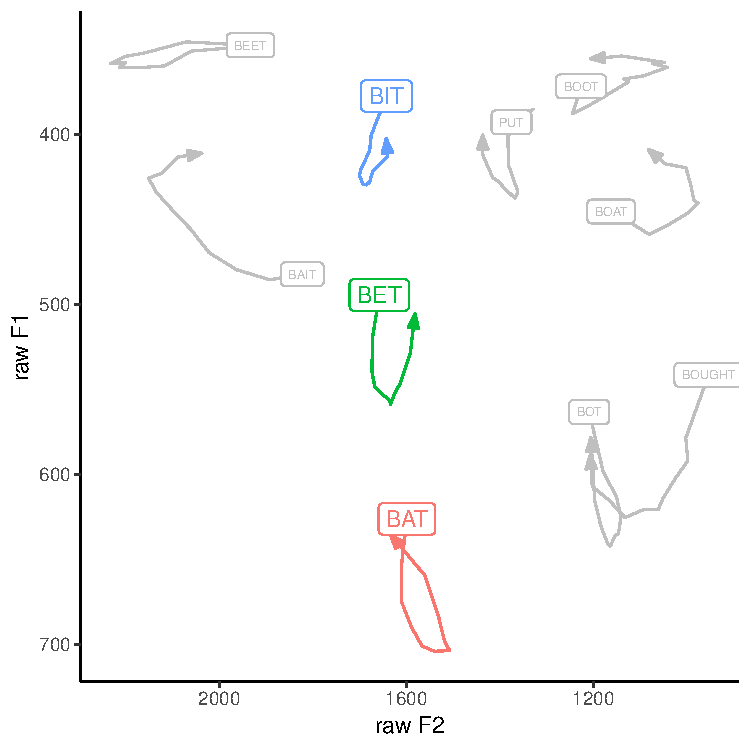
\includegraphics[width = \textwidth]{Figures/example_plots/51-Rich_avg_traj.pdf}
        \caption{Rich's trajectories are more U-shaped.}
        \label{fig:avg_traj_rich}
    \end{subfigure}
    \hspace{\fill}
    \begin{subfigure}[t]{2.925in}
        \centering
        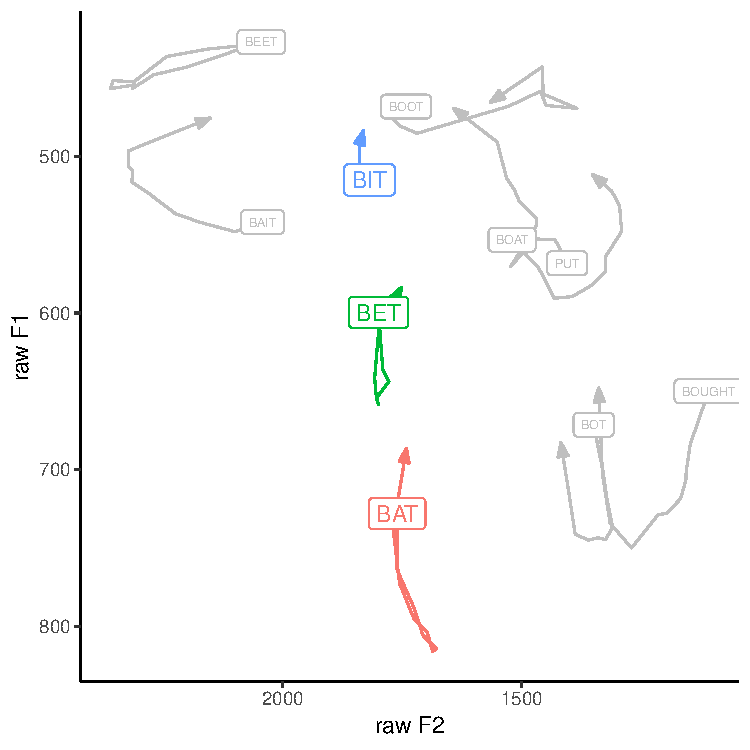
\includegraphics[width = \textwidth]{Figures/example_plots/54-Amber_avg_traj.pdf}
        \caption{Amber's trajectories are Bounce-shaped.}
        \label{fig:avg_traj_amber}
    \end{subfigure}
    \hspace{\fill}
    \caption{Average trajectories (in unnormalized Hz) for two Cowlitz County speakers showing the beginning and end stages of the Elsewhere Shift.}
    \label{fig:rich_and_amber}
\end{figure*}

The predicted values from the GAMMs however, are smoothed trajectories over many people. Does this claim hold up when the raw data is examined? Figure~\ref{fig:avg_traj_rich} shows the average trajectories for Rich, a male Boomer born in 1957. The trajectories of Rich's front lax vowels exhibit the characteristic narrow U-shape found in the older generations. In other words, while F1 gradually raises and then lowers, F2 undergoes a small amount of lowering. Meanwhile, Figure~\ref{fig:avg_traj_amber} is of Amber, a Millennial woman born in 1995. Here, we see a clear Bounce pattern that these models predict in the younger speakers: the F2 of these three vowels hardly changes at all and the trajectory changes in vowel height only.\footnote{It is difficult to compare the relative position of these speakers' vowels because the data is unnormalized. The only points of reference are the speakers' other vowels, but those too are in flux. However, compared to \fleece and \face, it appears that the lax vowels are lower in Amber's speech than in Rich's, supporting the chain shift as well.} These two speakers exemplify the change in trajectory shape and support the idea that the Elsewhere Shift is more than a change in position but is also change in vowel trajectory.

\begin{figure*}[tb!]
    \centering
    \hspace{\fill}
    \begin{subfigure}[t]{2.925in}
        \centering
        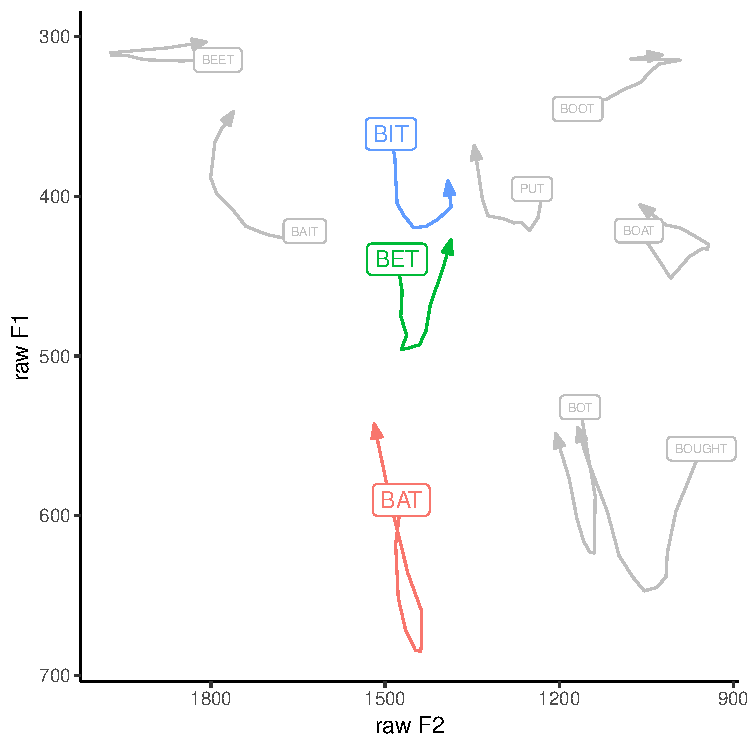
\includegraphics[width = \textwidth]{Figures/example_plots/30-Jason_avg_traj.pdf}
        \caption{Jason's \bat is ``bounced'' while \bet and \bit are U-shaped.}
        \label{fig:avg_traj_jason}
    \end{subfigure}
    \hspace{\fill}
    \begin{subfigure}[t]{2.925in}
        \centering
        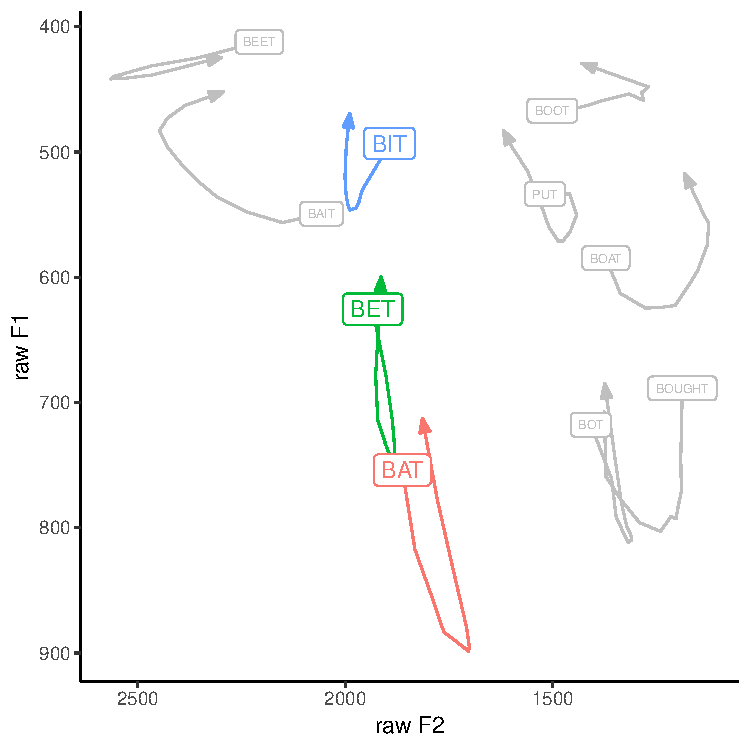
\includegraphics[width = \textwidth]{Figures/example_plots/29-Amanda_avg_traj.pdf}
        \caption{Amanda's \bat and \bet are ``bounced'' while \bit is U-shaped.}
        \label{fig:avg_traj_amanda}
    \end{subfigure}
    \hspace{\fill}
    \caption{Average trajectories (in unnormalized Hz) for two Cowlitz County speakers showing intermediate stages of the Elsewhere Shift.}
    \label{fig:jason_and_amanda}
\end{figure*}

The intermediate steps of this chain shift can also be found in these raw data plots. Figure~\ref{fig:avg_traj_jason} shows the average trajectories for Jason, a male from male from Gen X born in 1974. Jason's vowels show the first stages of the Elsewhere Shift with a Bounce-like pattern for \bat but not for \bet or \bit. Jason is one generation younger than Rich (Figure~\ref{fig:avg_traj_rich}) which supports the relative timing of the shift. Meanwhile, Figure~\ref{fig:avg_traj_amanda} shows the vowels of Amanda, a Millennial woman born in 1990. Here, both \bat and \bet have relatively little change in F2, while \bit is still U-shaped. Amanda appears to be a late adopter within her generation since \bit does not yet pattern with the other two vowels. These two speakers exemplify the intermediate stages of the Elsewhere Shift and show the relative timing of each vowel's changes.

\begin{figure*}[tb!]
    \centering
    \hspace{\fill}
    \begin{subfigure}[t]{2.925in}
        \centering
        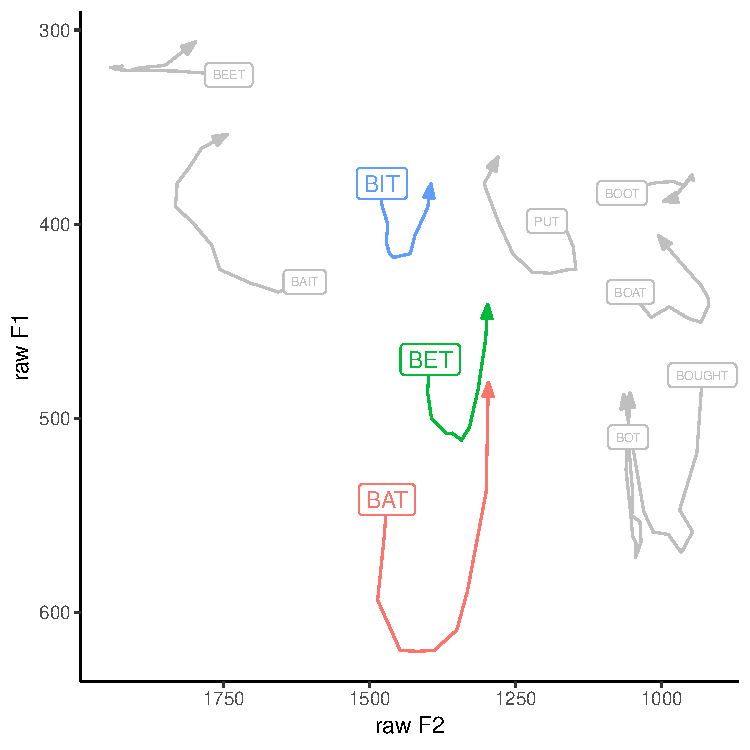
\includegraphics[width = \textwidth]{Figures/example_plots/35-Craig_avg_traj.pdf}
        \caption{Craig is a late adopter with his U-shaped trajectories.}
        \label{fig:avg_traj_craig}
    \end{subfigure}
    \hspace{\fill}
    \begin{subfigure}[t]{2.925in}
        \centering
        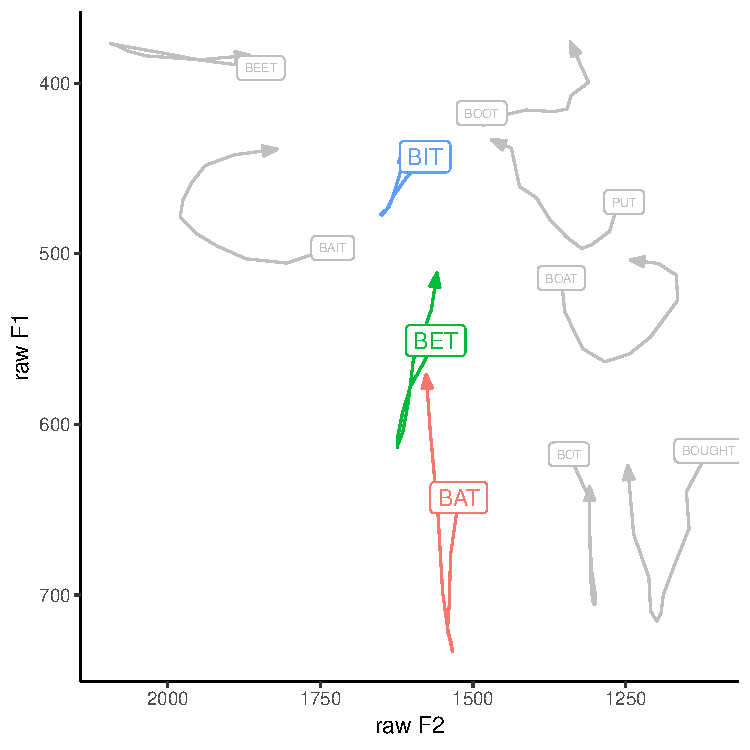
\includegraphics[width = \textwidth]{Figures/example_plots/47-Sean_avg_traj.pdf}
        \caption{Sean is an early adopter with his Bounce trajectories.}
        \label{fig:avg_traj_sean}
    \end{subfigure}
    \hspace{\fill}
    \caption{Average trajectories (in unnormalized Hz) for two Cowlitz County speakers.}
    \label{fig:craig_and_sean}
\end{figure*}

Two additional plots shed some light as to the social meaning of the Elsewhere Shift in Cowlitz County. Figure~\ref{fig:avg_traj_craig} shows the average trajectories of Craig, a male Boomer born in 1962. Despite other men his age adopting some of the shift (like Rich above), Craig appears to lag behind and exhibits clear U-shaped trajectories for all three front lax vowels. Meanwhile Figure~\ref{fig:avg_traj_sean} shows Sean, a Millennial man born in 1985. He is on the older end of his generation, but still has elements of the shift in all three vowels. Craig grew up in the rural north side of Cowlitz County, spoke fondly of the Longview's ``good ol' days,'' and rarely goes to Portland. Meanwhile, Sean grew up in the heart of Longview, expressed disdain towards Longview, and goes to Portland frequently to attend (or play in) concerts.\footnote{In Chapter~\ref{ch:discussion} we will hear more from both Craig and Sean and how they exemplify general community views towards Longview and Portland.} The correlation between their speech patterns and their views towards local places sheds some light on the social meaning of the Elsewhere Shift in Cowlitz County. This topic will be treated in more detail in Chapter~\ref{ch:discussion}.

Finally, I want to again point out the pattern found for \bet. While women were shifting the relative position of the vowel to a lower and more retracted position, both sexes were changing its shape from a U-shape to a bounce. Language change in Western cultures has shown that women are in the lead and that the men lag behind by a generation or so (as I have shown in this chapter). However, it may be that some aspects of the shift, namely the trajectories, advance equally in all social groups. While the men are not lowering or retracting \bet as the women are, the two sexes are in-step as they change the trajectory from a U to a Bounce. Additional work on trajectories in sound change are needed to see if this is a pattern found elsewhere, but it begs the question of how much information is missed when single-point measurements are used and trajectories are ignored.



\section{Conclusion}
\label{bat_bet_bit_conclusion}

This chapter has taken a close look at \bat, \bet, and \bit in Cowlitz County, Washington, giving particular emphasis on their trajectories. The front lax vowels are shifting in Cowlitz County, but the nature of the shift suggests a combination of a parallel shift and a pull chain. The relative timing of vowel lowering clearly indicates that \bat began shifting before \bet did, and that both vowels' movements are nearing completion. For \bit, there is evidence in the trajectory that it is beginning to shift as well in the Millennial women's speech. For all three vowels, the first half is shifting faster than the second half, causing a change in the trajectory shape from a U to a Bounce. In other words, there is less and less movement in F2 in these vowels in apparent time. These patterns are supported by examining data from individual speakers.

In conclusion, there is evidence to support both hypotheses stated in \S\ref{goals}: the Elsewhere Shift can be found in Cowlitz County, Washington and and it involves a change in trajectory as well as a change in position.
   % 6,358 words
\clearpage\chapter{Prenasal allophones of the front lax vowels}
\label{ch:prenasal}



This chapter presents the results of the GAMMs that were fit to the prenasal allophones of \trap, \dress, and \kit. First, I analyze \ban, \ben, and \bin in \S\ref{BAN}--\ref{BIN} and then I move to their pre-velar-nasal counterparts, \bang, \beng, and \bing in \S\ref{BANG}--\ref{BING}. A summary of findings regarding prenasal allophones in Cowlitz County and the prenasal split in general is found in \S\ref{sec:prenasal_discussion}. A more detailed discussion of how these patterns correlate to language-external effects in the region is found in Chapter \ref{ch:discussion}.

\section{\ban}
\label{BAN}

In this sample there were 2,588 tokens of \ban coming from 402 unique words. The most common words were \textit{family}, \textit{man}, \textit{grandma}, \textit{understand}, \textit{camp}, \textit{hand}, \textit{grandpa}, \textit{Kalama}, and \textit{ran}. There was an average of 44 tokens per speaker\footnote{Speakers ranged from 15 to 104 tokens with a standard deviation of 19.2: 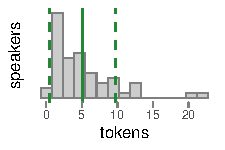
\includegraphics[width = 1.5in]{Figures/BANG/BANG_tiny.pdf}} and 324 per generation per sex. In Cowlitz County, the \ban vowel showed a number of large differences between social groups. Of the prenasal vowel classes, \ban was the one that I expected to exhibit the most social conditioning because of the patterns found in other communities in North American English. As this section will show, \ban was significantly affected by age and sex, putting Cowlitz County residents in line with other regions in the West.

\begin{figure*}[tb!]
    \centering
    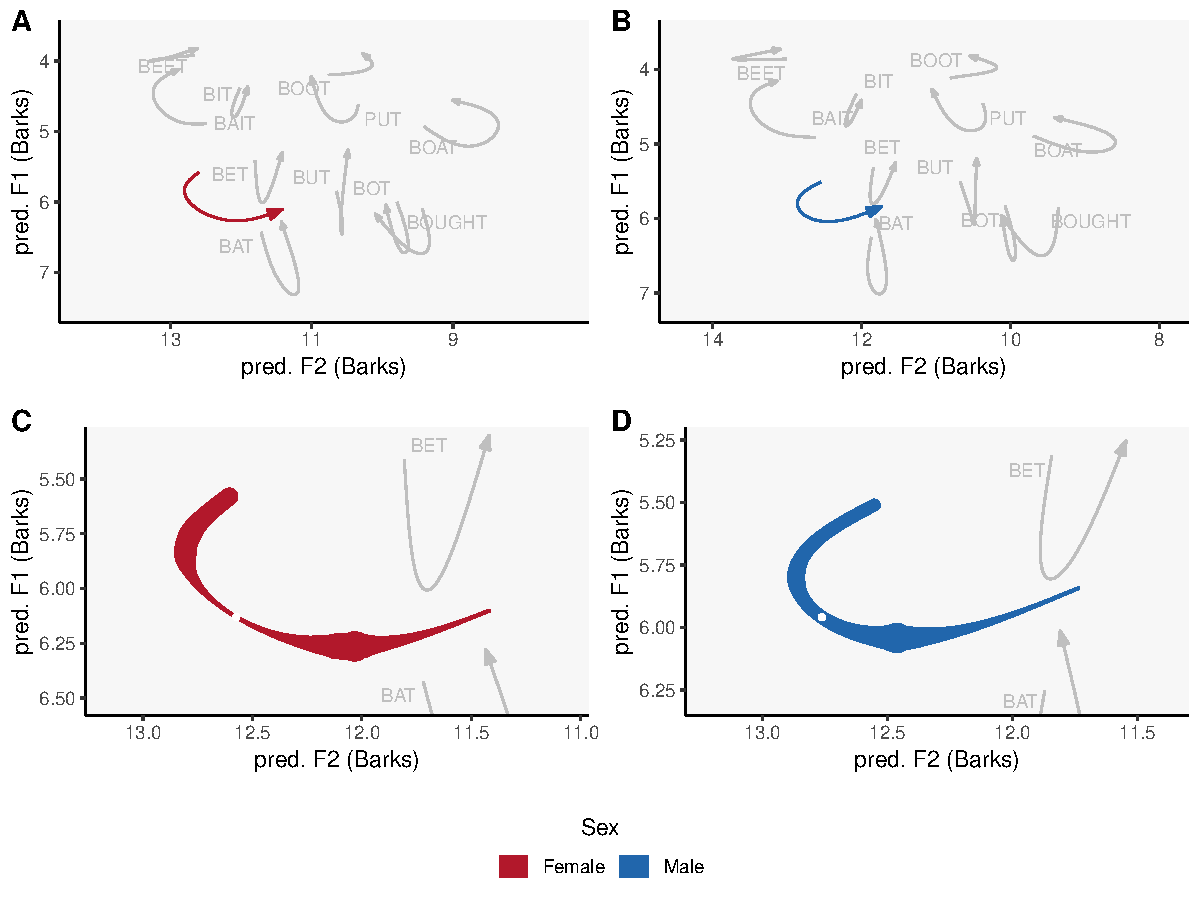
\includegraphics[width = 6.5in]{Figures/BAN/BAN_four_panel_plot_summarized.pdf}
    \caption[Predicted formant measurements for \ban by sex.]{Predicted formant measurements for \ban by sex with women on the left and men on the right. Predicted values are averaged across all generations.}
    \label{fig:BAN_four_panel_plot_summarized}
\end{figure*}

Figure \ref{fig:BAN_four_panel_plot_summarized} provides a general view of \ban's trajectory. The first thing to notice is the shape of \ban's curve. Recall that \bat was ``pointy'': it lowered and backed during the first half of its trajectory, had a clear target as both formants reversed directions, and then raised and fronted slightly towards the offset. In contrast \ban is much smoother. From its relatively higher and fronter onset, the trajectory begins with a gradual raising of F1 and F2; at about 30\% into the duration of the vowel, F2 reverses and begins lowering (causing a front-most peak in the trajectory) while F1 continues to raise; at about two-thirds into the duration, F2 is still lowering but F1 reverses and begins lowering, causing the trajectory to move higher and backer in the vowel space until the offset. Put more simply, F1 and F2 both rise and then fall, but their peaks are not lined up, resulting in a C-shaped trajectory in the F1-F2 space. An important consequence of this asynchrony is that the midpoint (the white dots in panels C and D of Figure \ref{fig:BAN_four_panel_plot_summarized}) are somewhat meaningless as they capture neither the frontest nor the lowest points of the trajectory. In fact, because \ban is quite dynamic throughout its entire duration, no single measurement can adequately capture its trajectory.

In addition to its general shape, these plots show that \ban is indeed raised in Cowlitz County. For both sexes, the vowel space occupied by these trajectories do not overlap at all with those of \bat. In fact, \ban is about the same height, though quite a bit more fronted, as \bet. Thus, a more accurate transcription of this vowel is fronted, nasalized mid-open front vowel with a lowered, nasalized mid-open offglide: [\textipa{\t{\|+{\~E}\textsubarch{\|`{\~E}}}}].

This description of \ban by Cowlitz County speakers matches closely with \citeauthor{swan_2016_proceedings}'s \citeyearpar[10--12]{swan_2016_proceedings} detailed account of the trajectory of \ban in the Pacific Northwest. The speakers from Seattle, who had a more raised variant than the those from Vancouver, began \ban relatively high and front in the vowel space, peaking in frontness about a third of the way though, and gradually lowered with significant backing along the course of its duration before raising again at some point during the last third of its trajectory. The similarity between these two communities is striking and hints at some uniformity across the state with regards to \ban.

\begin{figure*}[tb!]
	\centering
	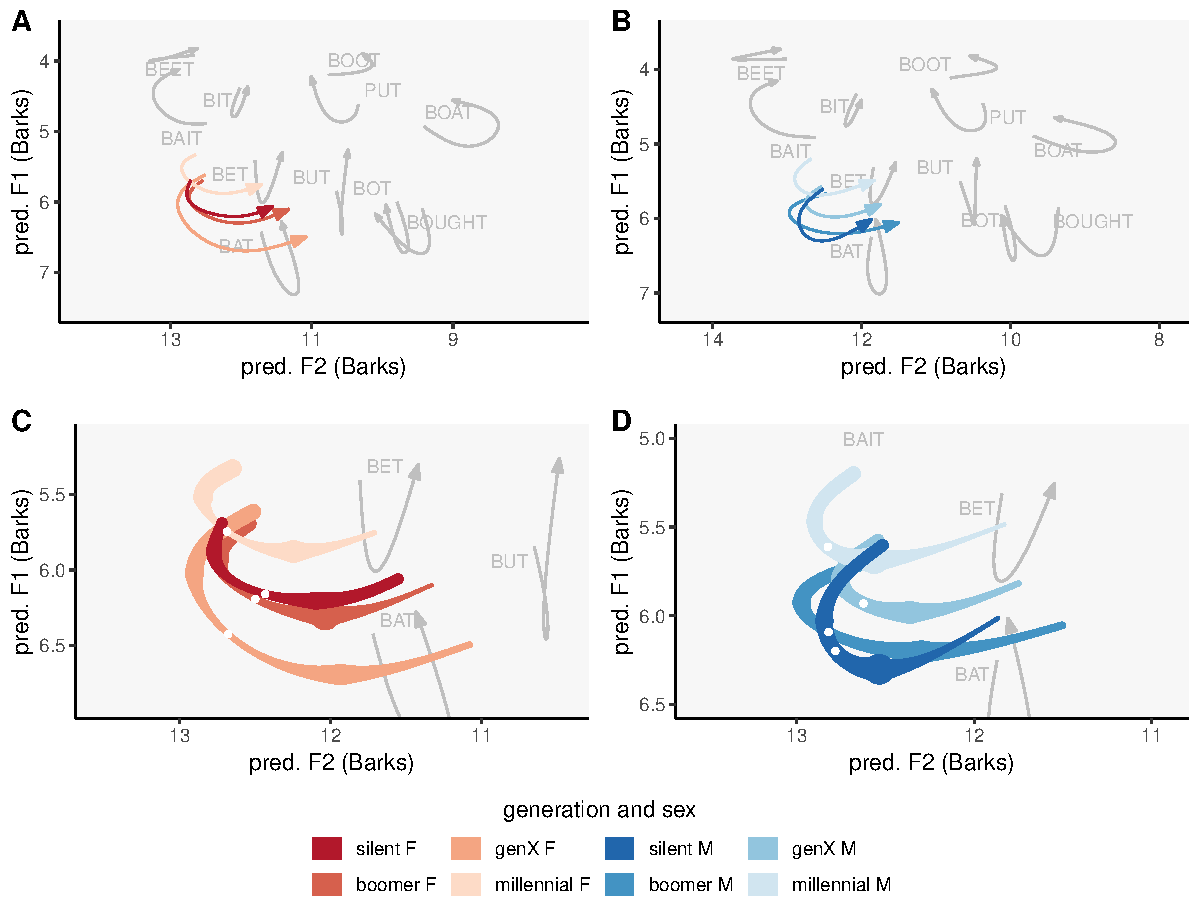
\includegraphics[width = 6.5in]{Figures/BAN/BAN_four_panel_plot.pdf}
	\caption[Predicted formant measurements for \ban by sex and generation.]{Predicted formant measurements for \ban by sex and generation. Women are on the left and men on the right. Darker shades represent older generations.}
	\label{fig:BAN_four_panel}
\end{figure*}

To visualize the effects of age on \ban, Figure \ref{fig:BAN_four_panel} augments the curves plotted in Figure \ref{fig:BAN_four_panel_plot_summarized} with additional trajectories for younger and older groups, illustrating two intriguing changes in apparent time. Beginning with the women, we see a unique reversal in the direction of language change. The oldest generation has a relatively high \ban, about as high as \bet but fronter. The Baby Boomer women were negligibly lower then the women in the Silent Generation (Appendix \ref{appendix:difference_smooths}, Figure \ref{fig:ban_diff_smooths_gen}A), suggesting that there was no change in this vowel before the 1960s. However, the women in Generation X used significantly lower and more diphthongal variants of \ban than the older two generations. Importantly, the bulk of this movement occurs during the offglide (namely the last third of the vowel's duration), while the onset is remaining stationary. As all of these plots do, panel C of \ref{fig:BAN_four_panel_plot_summarized} indicate the spectral rate of change with the thickness of the lines. Despite being a more dynamic vowel overall, the women in Generation X continue to spend a large amount of the duration of the vowel in the higher, fronter position before dropping down towards the offset, which also has the effect of pulling the midpoint towards the front (as evidenced by the thicker lines in panel C and the leftward shifting white dot).

This unusual pattern by the women in Generation X is supported in the raw formant measurements. Figure \ref{fig:kim_prenasal} shows the average trajectories used by Kim, a woman born in 1968. Kim's \ban vowel is drastically more diphthongal than her other prenasal vowels with a trajectory length\footnote{Because this calculation is based in raw data, the trajectory length is calculated by taking the sum of the euclidean distances between the 11 time points from which formants were extracted. These measurements are based on Bark-transformed normalized data.} of a staggering 4.10 Barks. Figure \ref{fig:holly_prenasal} shows another woman from Generation X who has a variant of \ban that is quite diphthongal (though not as extreme as Kim's) with a modest trajectory length of 3.26 Barks.

\begin{figure*}[tb!]
    \centering
    \hspace{\fill}
    \begin{subfigure}[t]{2.925in}
        \centering
        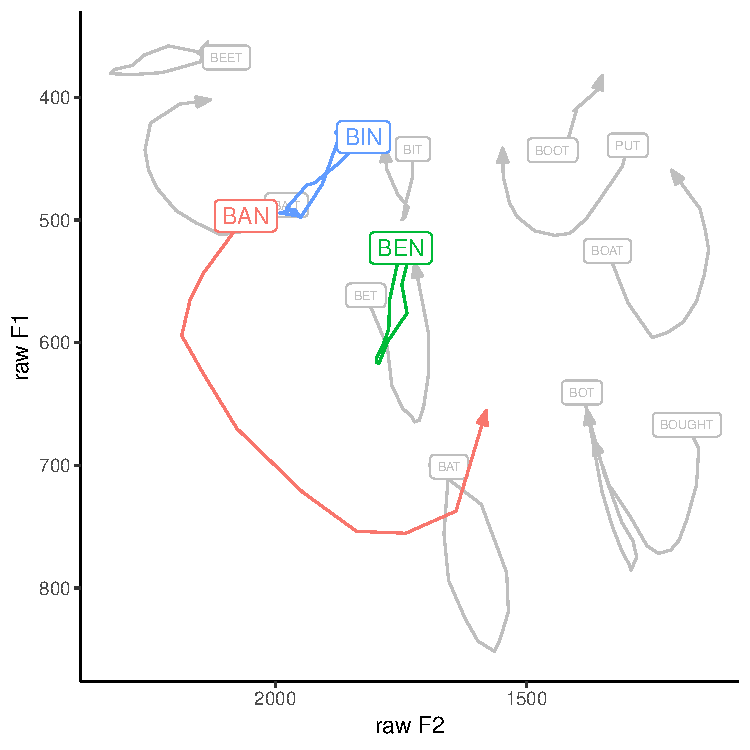
\includegraphics[width = \textwidth]{Figures/example_plots/24-Kim_avg_prenasal.pdf}
        \caption{Kim's prenasal vowels.}
        \label{fig:kim_prenasal}
    \end{subfigure}
    \hspace{\fill}
    \begin{subfigure}[t]{2.925in}
        \centering
        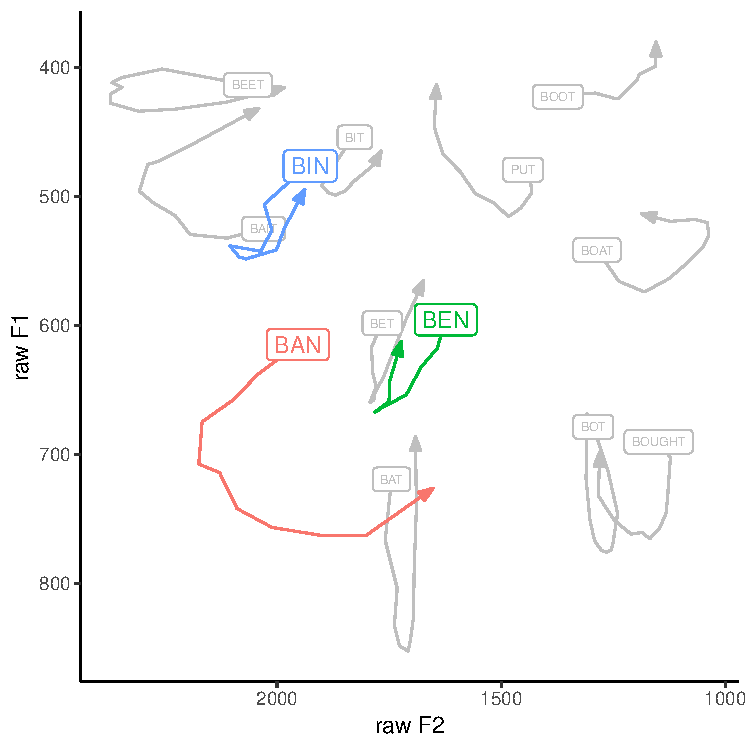
\includegraphics[width = \textwidth]{Figures/example_plots/48-Holly_avg_prenasal.pdf}
        \caption{Holly's prenasal vowels.}
        \label{fig:holly_prenasal}
    \end{subfigure}
    \hspace{\fill}
    \caption{Average trajectories (in normalized Hz) for two women in Generation X showing the diphthongal \ban vowel.}
    \label{fig:kim_and_holly}
\end{figure*}

This lowering by the women in Generation X drastically reverses when the Millennial women are added to the picture. These youngest speakers have a much higher realization of \ban---even higher than women of the Silent Generation. It was also quite a bit more monophthongal too: the trajectory length in the oldest two generations averaged was 1.75 Barks, in Generation X it was 2.72 Barks, and in the Millennials it was 1.57 Barks. So in this sample we see a pattern of stability, followed by lowering and diphthongization, and then followed by raising and monophthongization.

While the women undergo change in one direction with a quick reversal by the Millennials, the men appear to gradually raise \ban over the four generations. The right panels of Figure \ref{fig:BAN_four_panel_plot_summarized} show the men's predicted trajectories in shades of blue, with the oldest generation in the darkest shade. In stark contrast to the women's pattern, the oldest men had the lowest realization of \ban. And while women were stable or lowering \ban, this data suggests that the men were gradually raising it. This leads to the youngest generation which, like the women, have the highest variants of \ban. The difference smooths suggest no statistically significant amount of raising between any consecutive generation of men (\ref{fig:ban_diff_smooths_gen}C--D,O--P,W--X), but when the oldest two generations are compared to the Millennials, the latter 50\%--75\% of the trajectory is significantly higher (\ref{fig:ban_diff_smooths_gen}K,S).

\begin{figure*}[p]
	\centering
	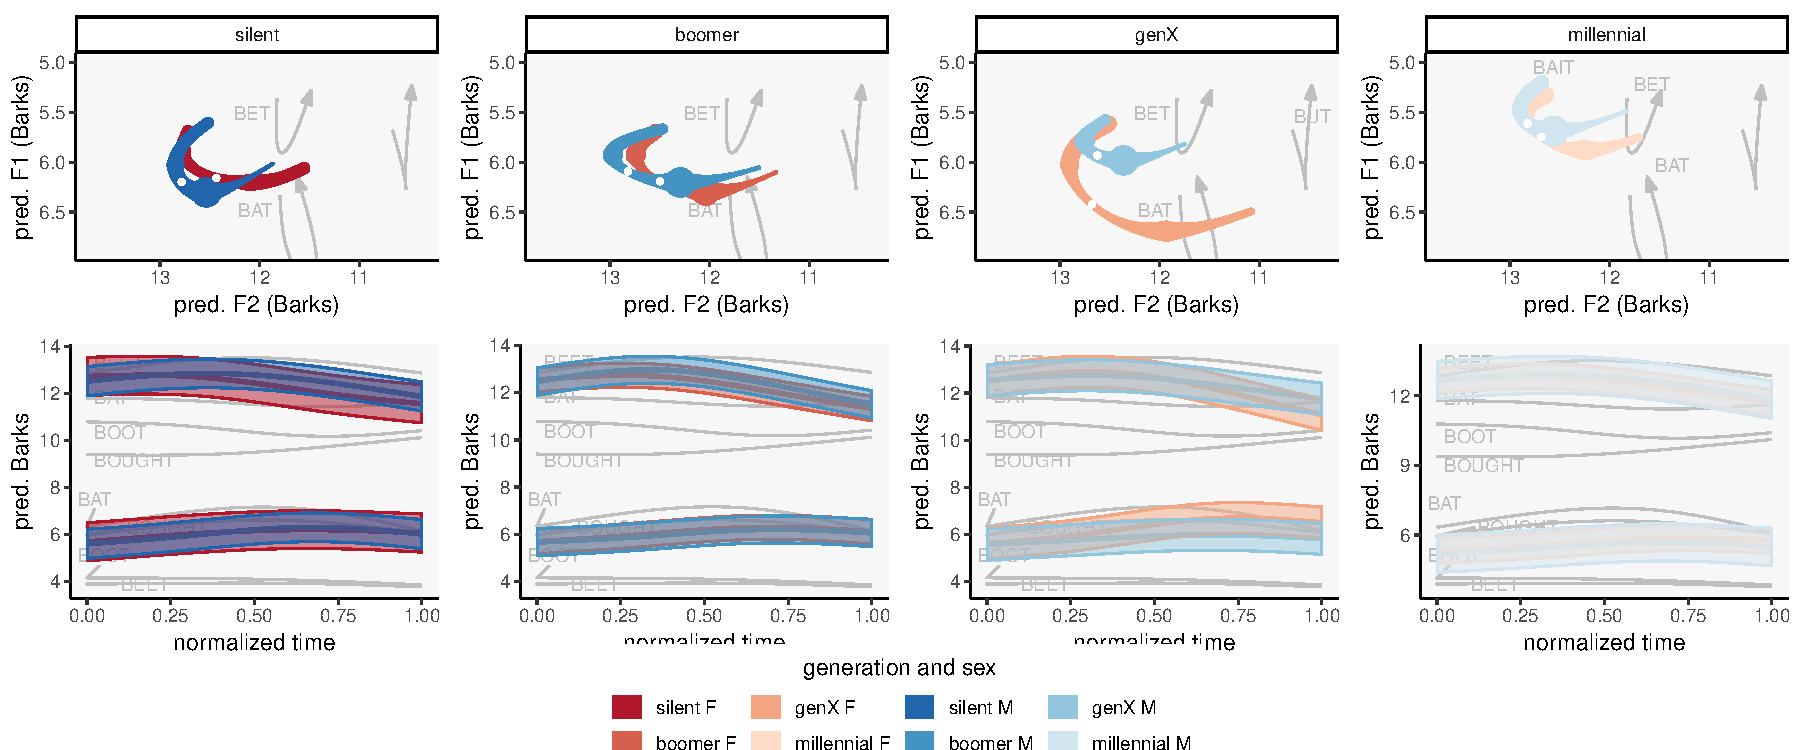
\includegraphics[angle = 90, origin = c, height = \textwidth]{Figures/BAN/BAN_sex_panel_plot_wide.pdf}
	\caption[Predicted formant measurements for \ban by generation.]{Predicted formant measurements for \ban by generation.}
	\label{fig:BAN_sex_panel_plot_wide}
\end{figure*}

By examining the generations one at a time and comparing the sexes within them, as in Figure \ref{fig:BAN_sex_panel_plot_wide}, we see additional support for the two patterns described above. In the Silent and Baby Boomer generations, the difference smooths show very little difference (\ref{fig:ban_diff_smooths_sex_gen}A--D). This sameness between the sexes coupled with no change across generations for both men and women suggests relative stability for the first two generations and that \ban was not undergoing language change at this time. But with Generation X, the men begin to raise \ban and the women lower it, resulting very large difference between the sexes in the second half of the vowel's trajectory (\ref{fig:ban_diff_smooths_sex_gen}E--F). Finally, the Millennial women raise \ban to catch up with the men, resulting in no statistically significant differences between them (\ref{fig:ban_diff_smooths_sex_gen}G--H). Other than Generation X, the two sexes are approximately the same in the four generations represented in this sample.

Summarizing \ban, we see that the general shape of \ban is similar to realizations recorded in Seattle (a C-shape) and that the primary dimension of change is in F1. With the exception of the women in Generation X, the overall pattern was that of raising. Women began lowering \ban in Generation X but then the Millennial-aged speakers raised it considerably. The men progressively raised \ban across all four generations.






\section{\ben}
\label{BEN}

In this dataset there were 4,445 tokens of \ben coming from 375 unique words. The most common words were \textit{went}, \textit{remember}, \textit{anything}, \textit{anyway}, \textit{ten}, \textit{many}, \textit{end(ed)}, \textit{twenty}, \textit{friend(s)}, and \textit{spent}. There was an average of 82 tokens per speaker\footnote{Speakers ranged from 23 to 250 tokens with a standard deviation of 36.4: 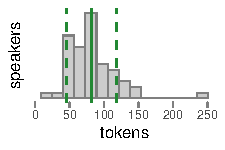
\includegraphics[width = 1.5in]{Figures/BEN/BEN_tiny.pdf}} and 556 per generation per sex. Like \ban, there are significant social effects that condition the realization of \ben, though this is primarily restricted to the women in this Cowlitz County sample.

\begin{figure*}[tb!]
    \centering
    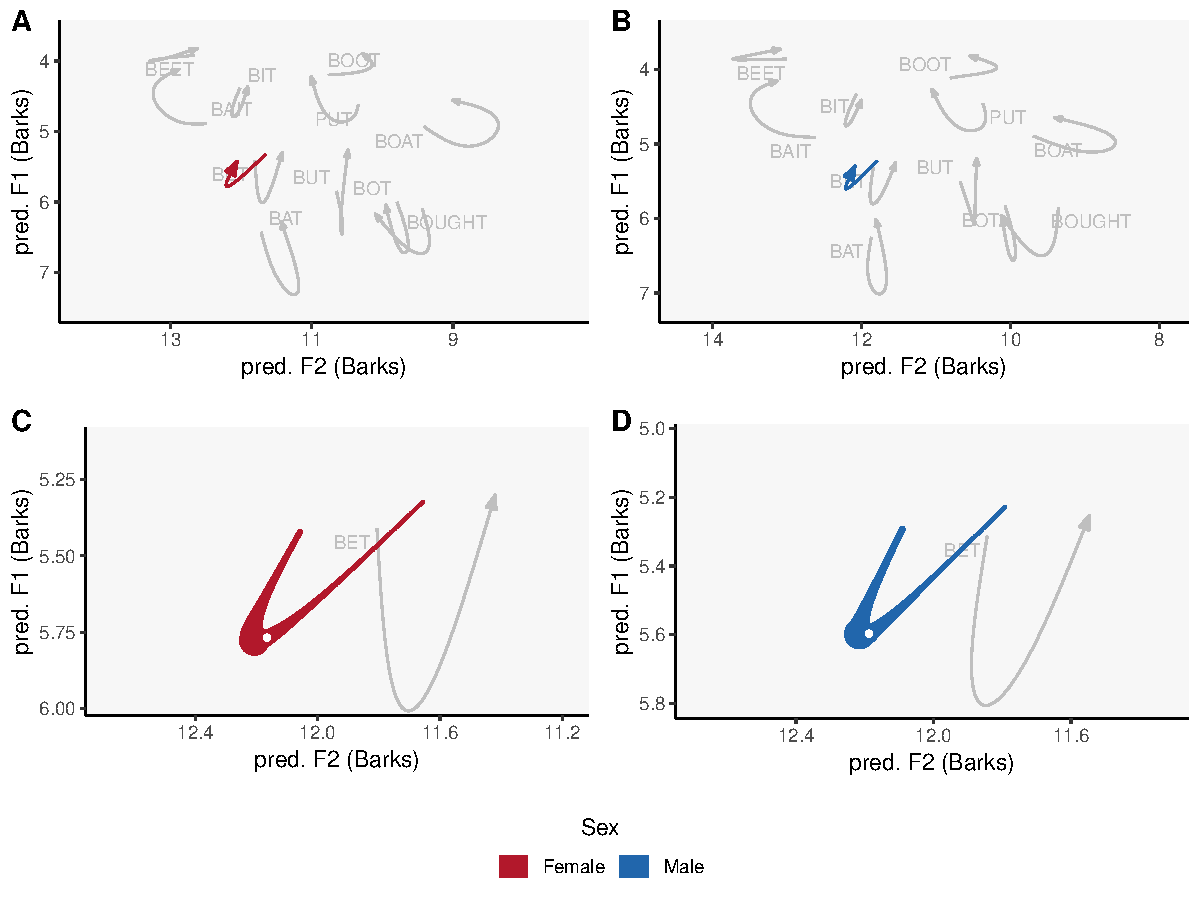
\includegraphics[width = 6.5in]{Figures/BEN/BEN_four_panel_plot_summarized.pdf}
    \caption[Predicted formant measurements for \ben by sex.]{Predicted formant measurements for \ben by sex with women on the left and men on the right. Predicted values are averaged across all generations.}
    \label{fig:BEN_four_panel_plot_summarized}
\end{figure*}

Figure \ref{fig:BEN_four_panel_plot_summarized} shows the effect of sex of \ben. There is relatively little difference between the sexes as far as relative position of the vowel or its shape, but its direction and shape are markedly different from the \ban (or \bin for that matter). Most notably, the offset is fronter than its onset, meaning this vowel is not ingliding as \bet is. As for its shape, as described previously, \ban has a characteristically smooth shape caused by the asynchrony of when F1 and F2 reverse directions. In stark contrast, \ben had a much ``pointier'' curve with the changes in F1 and F2 much more closely aligned. The vowel starts very near where \bet starts, but it lowers and fronts to its target, which is slightly fronter than \bet. After reaching its target, it reverses directions raises and retracts slightly towards if offset. Because of this vowel's clear target and relatively little movement in the F1-F2 space, I would consider this a monophthong, transcribed as [\textipa{\|+E}].

\begin{figure*}[tb!]
	\centering
	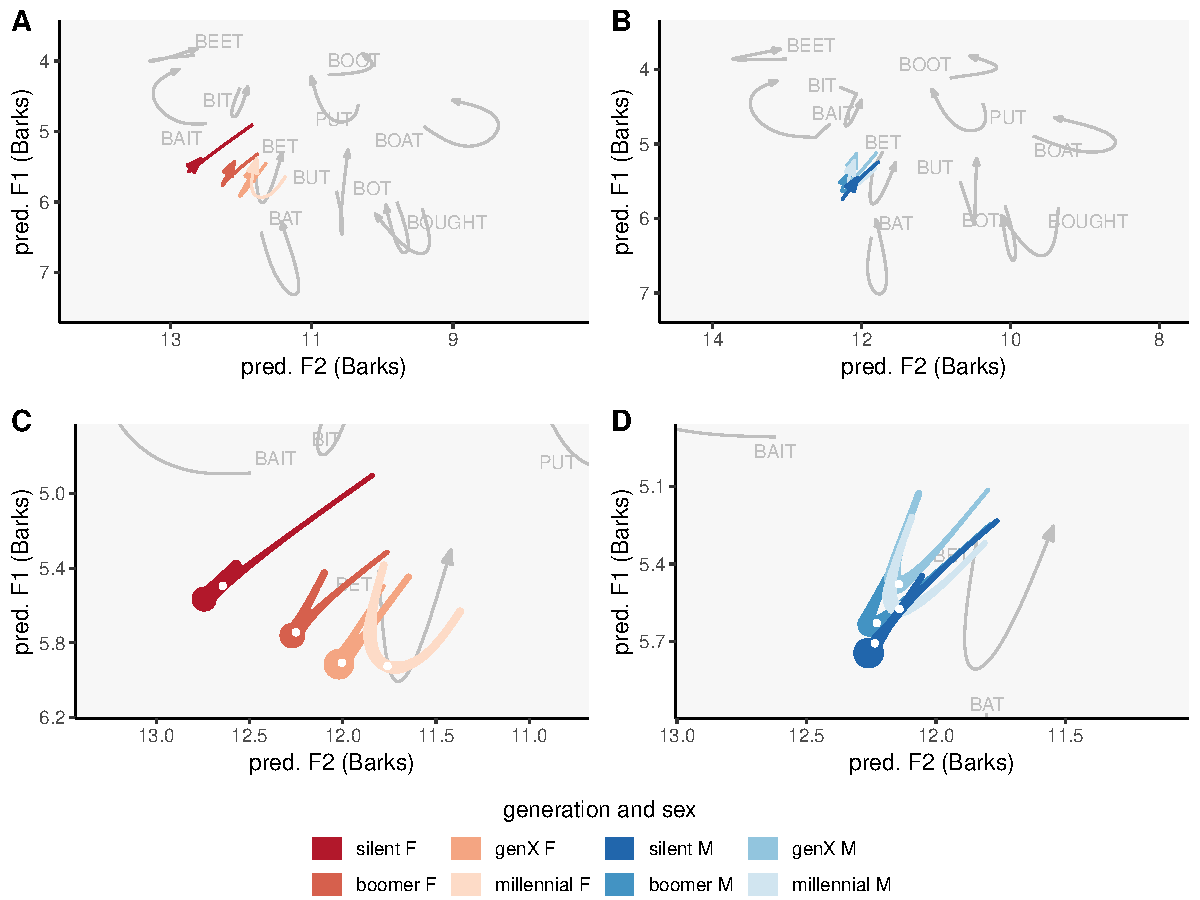
\includegraphics[width = 6.5in]{Figures/BEN/BEN_four_panel_plot.pdf}
	\caption[Predicted formant measurements for \ben by sex and generation.]{Predicted formant measurements for \ben by sex and generation. Women are on the left and men on the right. Darker shades represent older generations.}
	\label{fig:BEN_four_panel}
\end{figure*}

The interpretation of this vowel is complicated slightly when the data is split by generation, as in Figure \ref{fig:BEN_four_panel}. On the left, the women are clearly backing and slightly lowering the vowel in apparent time. The women of the Silent Generation had quite a fronted and raised variant of \ben but then the next two generations gradually retracted and lowered it.\footnote{Difference smooths suggest that this lowering happened primarily between the Silent Generation and the Baby Boomers (\ref{fig:ben_diff_smooths_gen}A).} Figure \ref{fig:ben_diff_smooths_gen} in Appendix \ref{appendix:difference_smooths} shows the difference smooths for these predicted values and suggests that the primary axis of change, which is statistically significant and relatively large, is along the F2 dimension (\ref{fig:ben_diff_smooths_gen}B,F,J,N,R). With each successive generation of women, the vowel was more centralized, to the point that the confidence intervals for the GAMM did not overlap for over half of the vowels' trajectory. Comparing non-adjacent generations only increases the differences. In fact, there was no overlap between the Millennial women's F2 in \ben and either the Baby Boomers' (\ref{fig:ben_diff_smooths_gen}R) or the women in the Silent Generation (\ref{fig:ben_diff_smooths_gen}J). So, it appears to be the case that \ben-retraction is robust in the women of this community and has been progressing actively for several generations. Meanwhile, there is some indication of \ben lowering in apparent time, but it was not as strong as the retraction. The difference between successive generations was not statistically significant in F1 (\ref{fig:ben_diff_smooths_gen}M,U), so it does not appear to be the case that children acquired a markedly different realization of \ben than their parents, at least in vowel height. However, when comparing the Silent with the Boomers and Gen X, there is a meaningful difference in the first half of the trajectory (\ref{fig:ben_diff_smooths_gen}A). Summarizing the movement of \ben in apparent time and the vowel space, a woman's \ben is more retracted than her mother's and more retracted and lower than her grandmother's.

In addition to their continued retraction, the Millennial women also drastically change the shape of the curve; the characteristic pointiness of the vowel is no longer present in the Millennial women's \bet and the changes in F1 and F2 are less abrupt, resulting in a more U-shaped pattern akin to \bet.

There is one more change that makes \ben stand out compared to the other vowels in this study: the time point of the peak F1. The women in the Silent generation achieve the highest F1 two-thirds into the vowel's duration. This is somewhat evident in panel C of Figure \ref{fig:BEN_four_panel} where the white dot representing the midpoint does not line up with the vowel's target.\footnote{This can also be seen in the spectrogram-like portion of the plots in Figure  (\ref{fig:ben_diff_smooths_gen}).} With each successive generation, this peak F1 shifts closer to the onset, such that the Millennial women's maximum F1 was about 44\% into the vowel's duration.\footnote{These numbers were found by extracting 501 points from the predicted trajectories of \ben for each generation and finding the time point that had the maximum F1.} So not only do the women lower, retract, and change the vowel's shape, but they are also altering when this nucleus is achieved.

For the men, there is little change. All four generations have very similar realizations of \ben that are in nearly identical positions in the vowel space, slightly fronter than \bet. Comparing the older three generations, there is a slight pattern of \ben raising in apparent time, with the Millennial men breaking the trend and lowering the vowel. The Millennial men also appear to have lost some of the pointiness to their curve and join their female cohorts in a more U-shaped pattern. Also, just like the women, the peak F1 also shifts earlier along the vowel's duration. However, the pairwise difference smooths between generations suggests no significant difference in either F1 or F2 between any two generations of men for \ben,\footnote{The one exception to this is the last third of the F1 differences between Silent men and Gen X men (\ref{fig:ben_diff_smooths_gen}G but I'm reluctant to call this a meaningful change.} so the differences, even spanning multiple generations, are small (\ref{fig:ben_diff_smooths_gen}, right two columns). Overall, Figure \ref{fig:BEN_four_panel} shows that the men are largely immune from the changes happening in the women's speech.

\begin{figure*}[p]
	\centering
	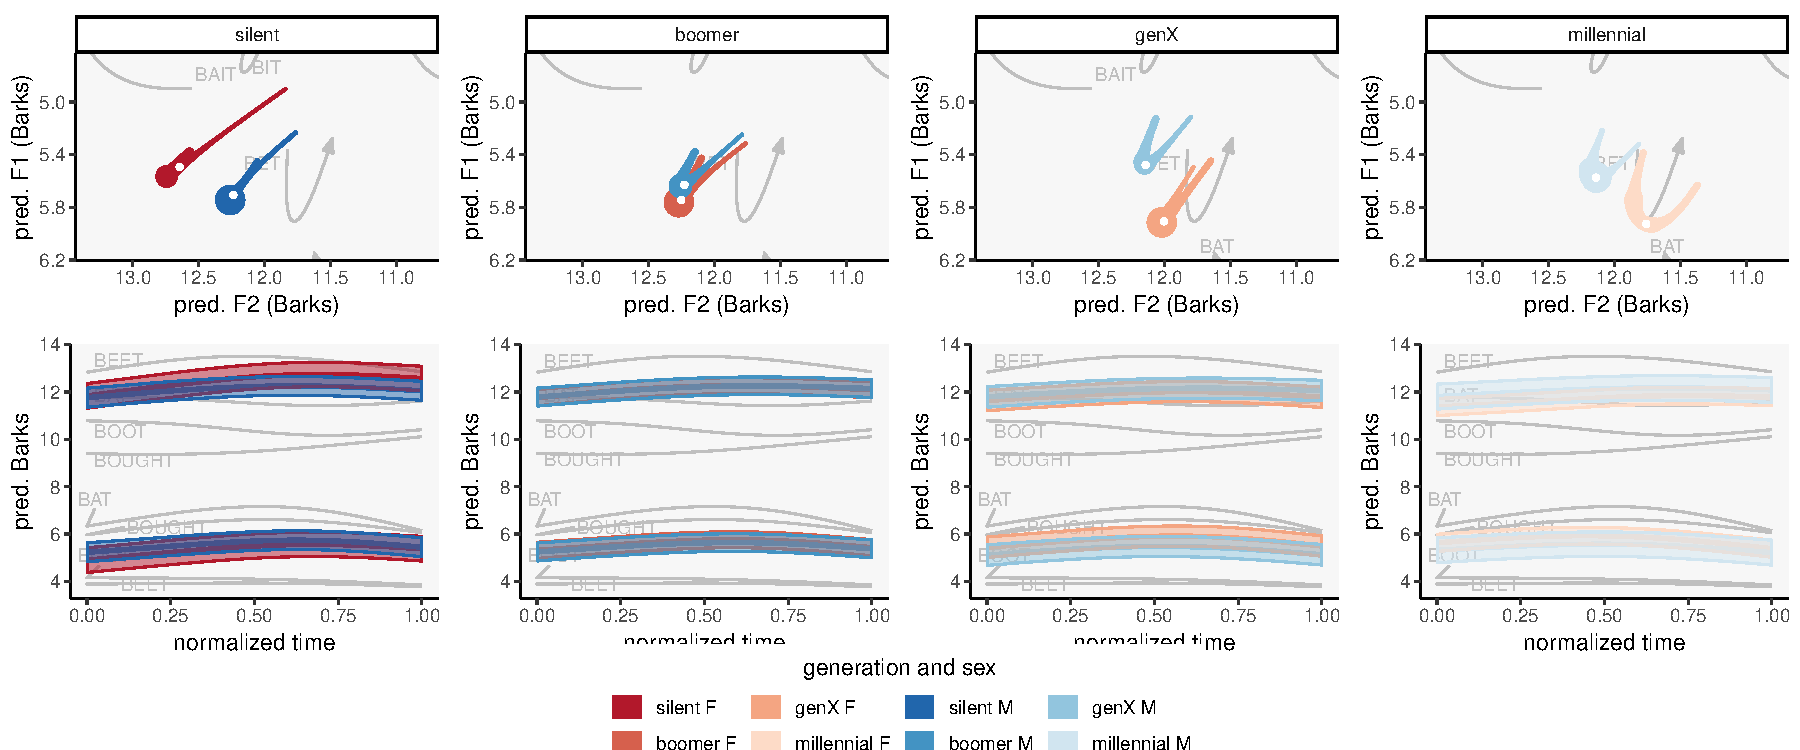
\includegraphics[angle = 90, origin = c, height = \textwidth]{Figures/BEN/BEN_sex_panel_plot_wide.pdf}
	\caption[Predicted formant measurements for \ben by generation.]{Predicted formant measurements for \ben by generation.}
	\label{fig:BEN_sex_panel_plot_wide}
\end{figure*}

When generations are isolated, as in Figure \ref{fig:BEN_sex_panel_plot_wide}, the amount of shifting in the women and the stability in the men becomes more apparent. In the Silent Generation, the women use more fronted variants (\ref{fig:ben_diff_smooths_sex_gen}B). In the Baby Boomers, difference smooths suggest no statistical significance (\ref{fig:ben_diff_smooths_sex_gen}C--D). But this similarity does not suggest the end of a shift because the women continue to lower and retract, and the difference smooths show almost no overlap in F1 between the two sexes (\ref{fig:ben_diff_smooths_sex_gen}E). Finally, with the Millennials, the women are more centralized compared to the men (the F2 difference smooth was statistically significant for its entire duration; \ref{fig:ben_diff_smooths_sex_gen}H) and quite a bit lower (F1 was lower for the first two-thirds of the trajectory; \ref{fig:ben_diff_smooths_sex_gen}G). In essence, Figure \ref{fig:BEN_sex_panel_plot_wide} shows that the men are relatively stable during the four generations here, but that women quickly shift past them. The question that remains then is why the sexes were so different in the Silent Generation. For now I leave this pattern in the Silent Generation as open question and hope that future research will help address this pattern.

The last thing that Figure \ref{fig:BEN_sex_panel_plot_wide} illustrates (better than Figure \ref{fig:BEN_four_panel} at least) is that the sexes had roughly similar trajectory shapes within generations. Specifically, the oldest generation has a ``point'' shaped trajectory, but over time, it becomes more U-like. Recall that this was also found with \bet, that even though the women steadily advanced their shift of the vowel, the shape of the men's vowel was remarkably similar as the women's. Again, this is not a product of the model because each combination of sex and generation was included as independent factor levels. It is even more remarkable that a finding that was unique to \bet (and not \bat or \bit) is also found for \ben (and not \ban or \bin). Thus it appears that there is some sort of pattern associated with \dress such that the men shift their trajectories in step with the women, but not the position of the vowel.

Summarizing \ben, this section showed that \ben were very different in shape than other prenasal tokens. To my knowledge, there is no detailed description of \ben in literature on Western English, so it is unclear whether these patterns are unique trends to this community or if can be found more broadly in the West. Regardless, the position of \ben changes in apparent time for the women, with younger generation successively lowering and retracting the vowel. However, both sexes smooth the trajectory out at the same time, going from a pointed shape to a U-shape.



\section{\bin}
\label{BIN}

The \bin vowel is defined as tokens of \bit before /\textipa{m}/ or /\textipa{n}/. In this corpus, there were 1,563 tokens of \bin coming from 265 unique words. The most common words were \textit{interesting}, \textit{since}, \textit{minutes}, \textit{timber}, \textit{dinner}, \textit{industry}, \textit{finished}, \textit{swimming}, \textit{cinnamon}, and \textit{inch}. In conversation, there was an average of 29 tokens per speaker\footnote{Speakers ranged from 5 to 72 tokens with a standard deviation of 12.3: 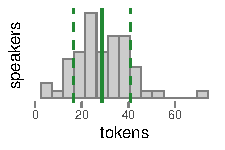
\includegraphics[width = 1.5in]{Figures/BIN/BIN_tiny.pdf}} and 195 per generation per sex. Compared to \ban and \ben, there is relatively little variation in \bin in Cowlitz County.

\begin{figure*}[tb!]
    \centering
    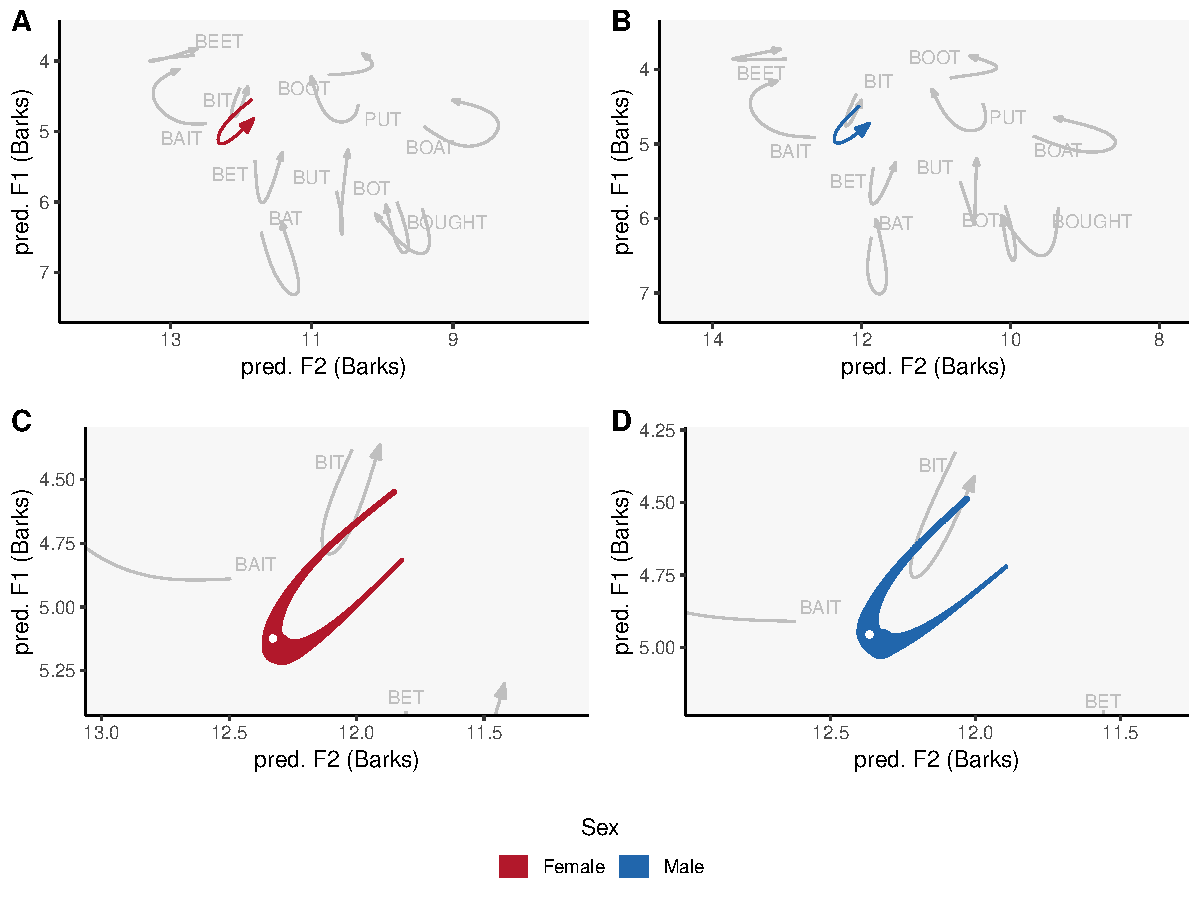
\includegraphics[width = 6.5in]{Figures/BIN/BIN_four_panel_plot_summarized.pdf}
    \caption[Predicted formant measurements for \bin by sex.]{Predicted formant measurements for \bin by sex with women on the left and men on the right. Predicted values are averaged across all generations.}
    \label{fig:BIN_four_panel_plot_summarized}
\end{figure*}

Figure \ref{fig:BIN_four_panel_plot_summarized} shows the overall shape of \bin and its position in the vowel space. The shape of this vowel's trajectory is similar to \ban: its C-shaped curve is caused by gradual changes in F1 and F2, with its lowest and frontest point being achieved about halfway into the vowel's duration. Overall the vowel does not traverse through much of the F1-F2 space, making it a relatively monophthongal (and lowered) [\textipa{\|`I}].\footnote{Its trajectory length was 1.29 Barks. For reference, \ben was more monophthongal on average at 1.01 Barks and \ban was more diphthongal at 1.80 Barks.} Continuing with the trend set by \ban and \ben, \bin is also fronter than its non-nasal counterpart. However, unlike \ban and \ben, \bin is actually lower in the vowel space than its corresponding elsewhere allophone, \bit.

\begin{figure*}[tb!]
	\centering
	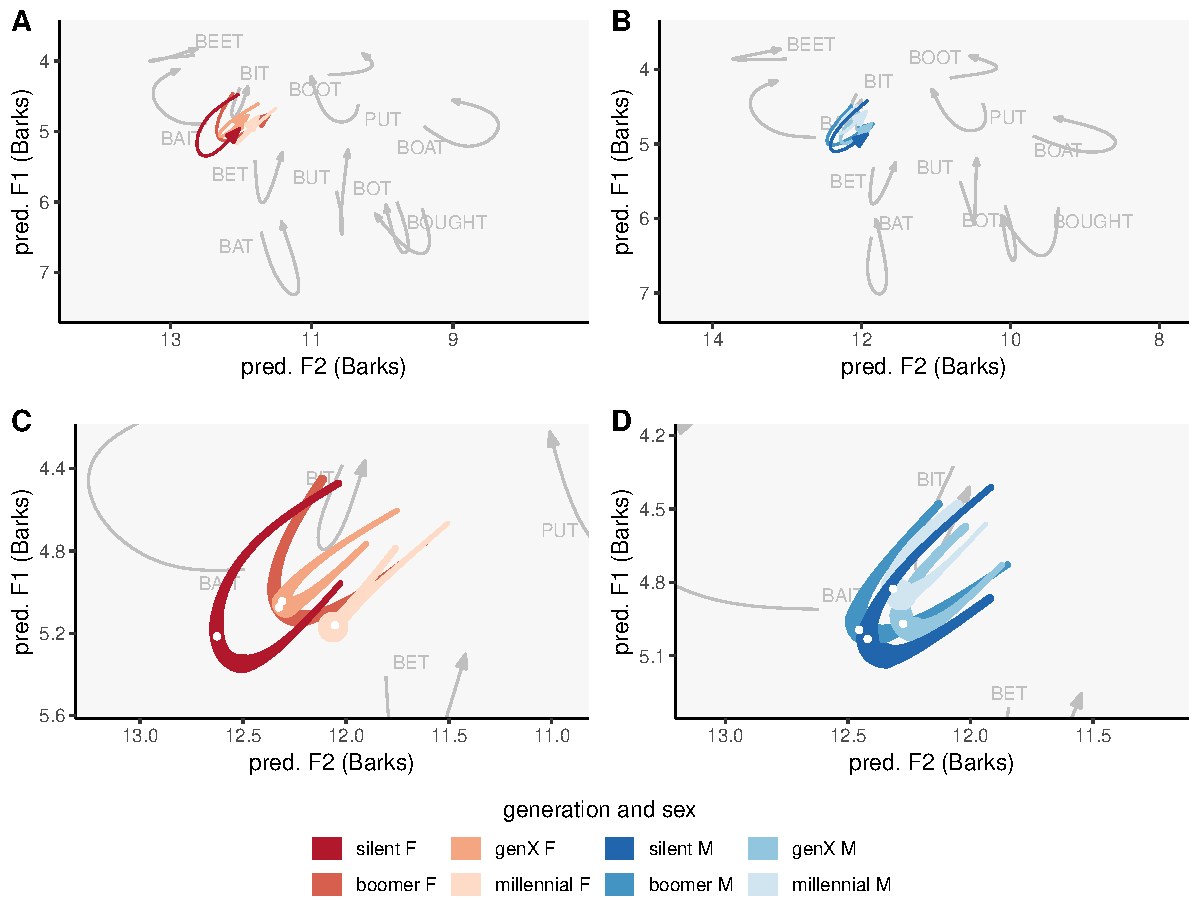
\includegraphics[width = 6.5in]{Figures/BIN/BIN_four_panel_plot.pdf}
	\caption[Predicted formant measurements for \bin by sex and generation.]{Predicted formant measurements for \bin by sex and generation. Women are on the left and men on the right. Darker shades represent older generations.}
	\label{fig:BIN_four_panel}
\end{figure*}

Figure \ref{fig:BIN_four_panel} shows how this realization changes in apparent time by sex. On the left, panels A and C indicate retraction and a change in the shape of \bin across the four generations of women. The oldest women had the most fronted and most dynamic variant of \bin. The realizations used by the Baby Boomer women was more or less the same as the women of the Silent generation only slightly retracted, though this difference was significant only at the very end of the vowel's duration (\ref{fig:bin_diff_smooths_gen}B). The Generation X women's realizations were approximately in the same vowel space as the Baby Boomers, but the vowel became less dynamic and developed a clearer nucleus; this difference between the middle generations was only significant in the portions closest to the onset and offset of the vowel, suggesting a change in shape more than a change in position (\ref{fig:bin_diff_smooths_gen}N). Finally, the Millennial women continued the trend and used the most centralized, the least dynamic,\footnote{The trajectory length in Barks for the Millennial women's \bin was 0.95 while the Silent women's was a full 50\% longer at 1.43.} and the pointiest variant of \bin. These changes with the Millennial women were significantly different from all three older generations of women, particularly in the first half of the vowel's duration in the F2 measurements (\ref{fig:bin_diff_smooths_gen}J,R,V). However, panel A of Figure \ref{fig:BIN_four_panel} shows that these changes all happen within a very small portion of the F1-F2 space. Like \bit, it appears then that the women are making small but significant changes to \bin by retracting it slightly and making the vowel less dynamic.

For the men, the pattern is similar to \bit: there is little evidence of change. Difference smooths show no statistically significant difference between any generation of the men's vowels at any point along their duration, for any pair of generations (\ref{fig:bin_diff_smooths_gen}, right two columns).

\begin{figure*}[p]
	\centering
	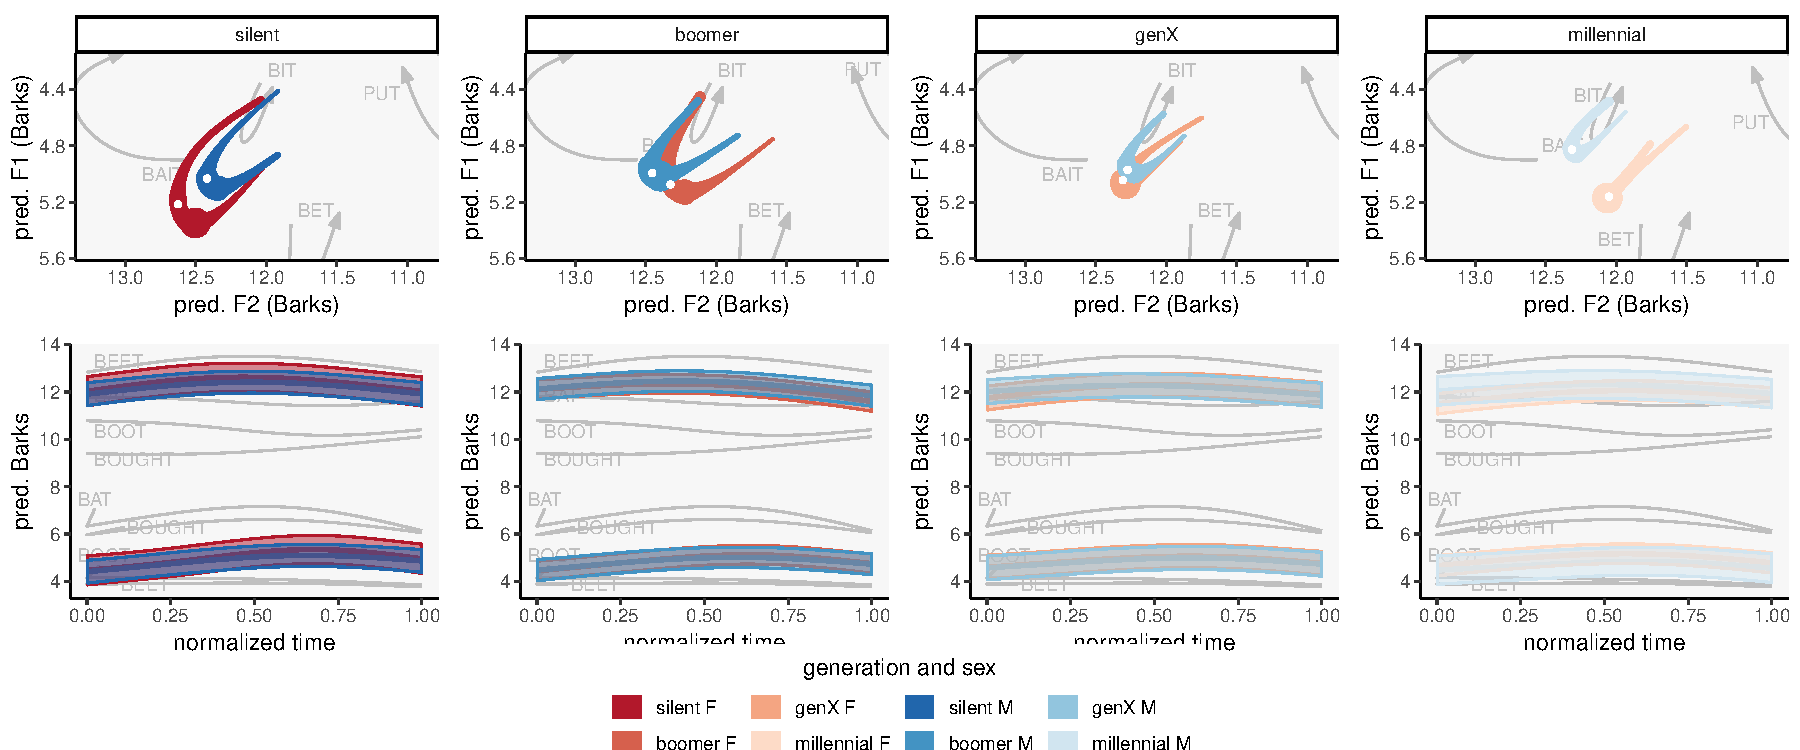
\includegraphics[angle = 90, origin = c, height = \textwidth]{Figures/BIN/BIN_sex_panel_plot_wide.pdf}
	\caption[Predicted formant measurements for \bin by generation.]{Predicted formant measurements for \bin by generation.}
	\label{fig:BIN_sex_panel_plot_wide}
\end{figure*}

Looking at \bin by generation, Figure \ref{fig:BIN_sex_panel_plot_wide} shows that the differences between the sexes was relatively small. For the first three generations, difference smooths suggest no statistically significant difference between men and women (\ref{fig:bin_diff_smooths_sex_gen}A--F). However, visually, it appears that the men's shape for \bin approximately matches the women's. Thus we have a bit of a paradox: the women show signs of change but the men do not, yet between the two groups there is no difference. This may simply be the result of the women's changes being so small in the vowel space. However, when the Millennials are examined, we see that the women's realizations are statistically lower during the middle half of the vowel (\ref{fig:bin_diff_smooths_sex_gen}G), and more retracted during the first 40\% (\ref{fig:bin_diff_smooths_sex_gen}H). Thus we have a situation where there is relative stability for three generations, with the only change being in the shape of the vowel's trajectory, but then the Millennial women suddenly begin lowering and retracting the vowel.

In summary, \bin was realized slightly lower than \bit and the shape of the vowel was more U-shape, like \ban, though it was much less dynamic and was contained a relatively small portion of the vowel space. For the women, there was a small but significant indication of retraction and monophthongization in apparent time with the Millennial women shifting the vowel the most. For the men, there was no evidence of change.

\section{Interim summary}

So far, this chapter has described the patterns found in \ban, \ben, and \bin (the pre-/\textipa{m}/ and pre-/\textipa{n}/ tokens of \trap, \dress, and \kit). For \ban, both sexes gradually raised it with the exception of the Generation X women who lowered it. For \ben, the women lower and retract it while changing its shape. \bin did not lower but the women appear to retract it by a small amount. Thus we see shifting in three different directions. There was no evidence of apparent time change in the position of men's realizations of \ben or \bin, but their curves became pointier. In many cases for both sexes, the vowel does not shift in the F1-F2 space, but instead it becomes more monophthongal.

The next three sections treat a different subset of prenasal tokens, \bang, \beng, and \bing, to identify changes that occur before pre-velar-nasal front lax vowels.








\section{\bang}
\label{BANG}

In this sample, there were 275 tokens of \bang coming from 56 unique words. The most common words were \textit{language}, \textit{thank(s)}, \textit{hang(ing)}, \textit{Da Nang},\footnote{Da Nang is a city in Vietnam that had a U.S. Air Force base during the Vietnam War. One speaker told stories of when he served there.} \textit{tank}, \textit{angry}, \textit{bank} and \textit{ankle}. There was an average of 5 tokens per person,\footnote{Of the speakers that produced any \bang tokens, they ranged from 1 to 22 tokens with a standard deviation of 37.1: 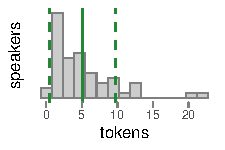
\includegraphics[width = 1.5in]{Figures/BANG/BANG_tiny.pdf} Two speakers, Laura (female Boomer) and Dale (male Silent), did not use any tokens of 10 \bang.} and 34 per generation per sex. This is admittedly not a lot of data to be working with, but the results of the GAMMs are reasonable and coincide with my intuitions of the data.

\begin{figure*}[tb!]
    \centering
    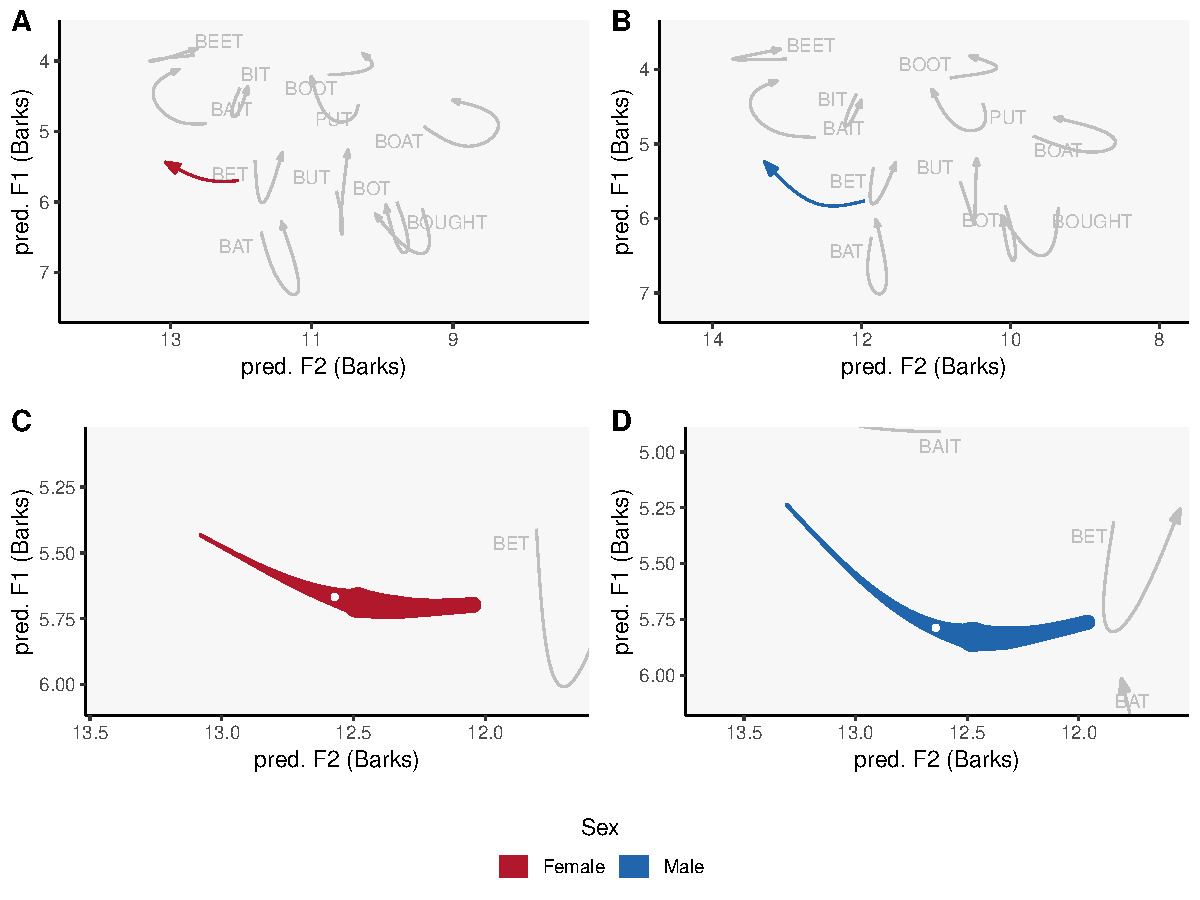
\includegraphics[width = 6.5in]{Figures/BANG/BANG_four_panel_plot_summarized.pdf}
    \caption[Predicted formant measurements for \bang by sex.]{Predicted formant measurements for \bang by sex with women on the left and men on the right. Predicted values are averaged across all generations.}
    \label{fig:BANG_four_panel_plot_summarized}
\end{figure*}

Figure \ref{fig:BANG_four_panel_plot_summarized} show a general plot for \bang. First, it is clear that the shape of this vowel's trajectory is different from the others in that there is relatively little movement in F1 and that almost all of the change is in F2. This is undoubtedly a result of the velar pinch, which causes a sharp rise in F2 as the back of the tongue raises to form the velar consonant. It is difficult to determine the precise target for this vowel since there is no real steady state. Not only does this make any one measurement somewhat arbitrary, it suggests that this vowel may be characterized by the overall position and shape of its trajectory rather than by a single point in the vowel space. Transcribed into IPA, this vowel is [\textipa{\t{\~E\textsubarch{\|+{\|'{\~E}}}}}]\vspace{-0.35em}, a nasalized mid-open diphthong, with a raised and fronted offglide.
% Nice hack to correct the extra line spacing when the stacked diacritics adjusted the baseline height. 0.35em is just eyeballing it and it looks pretty good even when zoomed way in. It was also

\begin{figure*}[tb!]
	\centering
	\includegraphics[width = 6.5in]{Figures/BANG/BANG_four_panel_plot.pdf}
	\caption[Predicted formant measurements for \bang by sex and generation.]{Predicted formant measurements for \bang by sex and generation. Women are on the left and men on the right. Darker shades represent older generations.}
	\label{fig:BANG_four_panel}
\end{figure*}

When the data is split up by generation (Figure \ref{fig:BANG_four_panel}), the shape of the vowel's curve is similar across all ages, though its relative height and the degree of fronting varies in a somewhat haphazard way. Beginning with the women, we see that the older three generations do not change their realizations of \bang in an appreciable way. The shapes differ slightly, but the difference smooths suggest that they are not significant (\ref{fig:bang_diff_smooths_gen}A--B,E--F,I--J,M--N). However, like other vowels, the Millennial women exhibited the most amount of change. They had the highest, most retracted, and most monophthongal realizations of \bang. This shift was significant in F1 along most of the first half of the vowel (\ref{fig:bang_diff_smooths_gen}Q,U) and in F2 along the second half (\ref{fig:bang_diff_smooths_gen}R,V). On average, the older three generations' trajectory lengths for \bang was 1.28 Barks while for the Millennial women it barely over half that at 0.67 Barks.

The men in Cowlitz County meanwhile shifted \bang more gradually. The difference between any two consecutive generations was insignificant (\ref{fig:bang_diff_smooths_gen}C--D,O--P,W--X), but comparing the Silent men to the Millennial men, the first 20\% of the duration is primarily where the difference lies (for both F1 and F2; \ref{fig:bang_diff_smooths_gen}K--L). The pattern of monophthongization was also apparent, and occurred gradually from 2.01 Barks in the Silent men to 1.17 in the Millennials. Interestingly, as they raise the vowel, the men keep the offsets approximately in the same place while fronting the onset, resulting in that significant difference in F2. The women meanwhile keep the onset approximately the same while ending the offglide earlier, resulting in a slightly more retracted \bang.

\begin{figure*}[p]
	\centering
	\includegraphics[angle = 90, origin = c, height = \textwidth]{Figures/BANG/BANG_sex_panel_plot_wide.pdf}
	\caption[Predicted formant measurements for \bang by generation.]{Predicted formant measurements for \bang by generation.}
	\label{fig:BANG_sex_panel_plot_wide}
\end{figure*}

This shift in opposite directions is more apparent in Figure \ref{fig:BANG_sex_panel_plot_wide}, which compares men and women in the same generation. The difference between the sexes was slight and none of the difference smooths here came out significant (\ref{fig:bang_diff_smooths_sex_gen}).\footnote{The one exception was a very small portion near the onset of the F2 differences in the Silent generation, but I am hesitant to call that a meaningful difference.} So, when interpreting this pattern of men fronting \bang and women retracting it, care should be taken. The low token count likely accounts for the large confidence intervals and additional study that focuses on extracting many tokens of \bang will be necessary to substantiate this pattern.





\section{\beng}
\label{BENG}

In \S\ref{word_classes} I explain that there are very few tokens of \beng in English. In a study of the front lax vowels in California, \citet[40]{cardoso_etal_2016_pads} were forced to exclude this vowel class from analysis because there was only one token from their sample of 22 speakers. In Cowlitz County, I collected only 76 tokens of \beng, though this was primarily through the ``Cat and the Mice'' passage which contained the words \textit{length} and \textit{strength}. In conversation there were an additional five tokens of \textit{lengths}, three of both \textit{length} and \textit{strength}, and one each of \textit{lengthy} and \textit{strengthen}. Because there are so few tokens (and none by Millennial men), a robust analysis of \beng using GAMMs is not possible.

\begin{figure*}[tb!]
	\centering
	\includegraphics[width = 3.25in]{Figures/BENG/BENG_raw.pdf}
	\caption[Average trajectories for \beng by generation.]{Average trajectories for \beng by generation based on normalized formant measurements (not predicted values), transformed into Barks. Unlike every other plot in this study, this figure includes data from the reading passages.}
	\label{fig:BENG}
\end{figure*}

I can only provide a small glimpse into what this vowel is like. Figure \ref{fig:BENG} shows the normalized values for \beng, averaged for each generation. Data from the reading passages was included because only 12 tokens of \beng occurred in conversation. This plot shows that the
\beng vowel begins with quite a low F2, but this is likely due to the fact that every token of \beng in this corpus is preceded by light /\textipa{l}/ or /\textipa{\*r}/, which are characterized by their low F2 values \citep{olive_etal_1993}. This predictable consonantal effect makes comparison with \bang and \bing difficult, at least with respect to the onset of F2. Other than this longer trajectory, \beng appears to share properties with \bang: the trajectory is primarily along the F2 dimension, it is about the same height as \bet. The offset of \beng is approximately as front as \bit while \bang goes as far front as \fleece. In IPA, \beng is [\textipa{\t{\=*{\~E}\textsubarch{\|+{\~E}}}}]: a retracted, nasalized mid-open vowel with a fronted, nasalized mid-open offset.

Without additional data, generalizations are only speculative at this point. Because their trajectories overlap in the vowel space, it is possible that \beng and \bang are merged.\footnote{Impressionistically, the \bang and \beng are very close and possibly merged.} However, \beng appears slightly more centralized then \bang, both at the onset and the offset, but this may be the result of coarticulatory effects. Because of the extremely limited set of words containing \beng, additional study---possible one that analyzes the realization of nonce words with \beng---is needed to fully understand this vowel. Further analysis on this vowel in Cowlitz County will be saved for future analysis.






\section{\bing}
\label{BING}

Finally, the last vowel to be described in this chapter is \bing, or rather, \kit before velar nasals. This corpus has 2,222 tokens of \bing coming from 85 unique words. There were actually more observations of \bing than \bin, but they come from fewer tokens. The most frequent words by a large margin were \textit{think} and \textit{thing(s)}, which were followed by \textit{thinking}, \textit{bring}, \textit{single}, \textit{English}, \textit{drink}, \textit{spring}, and \textit{sing}, and \textit{ring}. There was an average of 41 tokens of \bing per person\footnote{Speakers ranged from 11 to 168 tokens with a standard deviation of 24.5: \includegraphics[width = 1.5in]{Figures/BING/BING_tiny.pdf}} for an average of 278 per generation per sex. Like \bin, this vowel exhibits relatively few changes across social groups in Cowlitz County.


% There's really no good place to put this.
\begin{figure*}[tb!]
    \centering
    \includegraphics[width = 6.5in]{Figures/BING/BING_four_panel_plot_summarized.pdf}
    \caption[Predicted formant measurements for \bing by sex.]{Predicted formant measurements for \bing by sex with women on the left and men on the right. Predicted values are averaged across all generations.}
    \label{fig:BING_four_panel_plot_summarized}
\end{figure*}

Figure \ref{fig:BING_four_panel_plot_summarized} shows the trajectory of \bing relative to non-nasal allophones of the other vowels. The shape of the trajectory is similar to \bang where there is a large raise in F2, reflecting the velar pinch, but \bing has more change in F1 over its duration (and a clearer target) than \bang or \beng. For both sexes, \bing occupies nearly the same position in the vowel space as \face, which is fronter than \bit and at the same height. In IPA, this vowel is a nasalized, high front lax vowel with a fronted, nasalized, high lax offglide:  [\textipa{\t{\~I\textsubarch{\~{\|+I}}}}].

\begin{figure*}[tb!]
	\centering
	\includegraphics[width = 6.5in]{Figures/BING/BING_four_panel_plot.pdf}
	\caption[Predicted formant measurements for \bing by sex and generation.]{Predicted formant measurements for \bing by sex and generation. Women are on the left and men on the right. Darker shades represent older generations.}
	\label{fig:BING_four_panel}
\end{figure*}

When splitting the data up by generation, as in Figure \ref{fig:BING_four_panel}, there are differences between how the women and men changed their realizations of \bing in apparent time. Beginning with the women, there is no appreciable change in height between generations, though there is some change in F2. Recall that for \bin, the women centralized the vowel slightly in apparent time while making it less diphthongal. Likewise, there was no statistical significance among the the oldest three generations' realizations of \bing at all (\ref{fig:bing_diff_smooths_gen}A--B,E--F,M--N). However, the Millennial women had the most centralized variant and difference smooths suggest that this fronting, compared to all three previous generations, is statistically significant (\ref{fig:bing_diff_smooths_gen}J,R,V). It appears that \bing is retracting in apparent time just as \bin and \bit are and that and this change may have started relatively recently.

In contrast, this backing is not found in the men's data. Figure \ref{fig:BING_four_panel} shows that the Generation X and Millennial-aged men had a higher variant of \bing. In addition \bing gets less dynamic as trajectory lengths for the older two generations averaged 2.17 Barks while for the younger generation it was only 1.23 Barks. Difference smoooths suggest some fronting in the younger generation (\ref{fig:bing_diff_smooths_gen}L,T), but it was only in the onset of the vowel, which is more indicative of the shorter trajectory rather than fronting of the entire vowel. Compared to \bin, there is a clearer change in apparent time for men's realizations of \bing, which justifies treating these two variables separately.

\begin{figure*}[p]
	\centering
	\includegraphics[angle = 90, origin = c, height = \textwidth]{Figures/BING/BING_sex_panel_plot_wide.pdf}
	\caption[Predicted formant measurements for \bing by generation.]{Predicted formant measurements for \bing by generation.}
	\label{fig:BING_sex_panel_plot_wide}
\end{figure*}

Finally, Figure \ref{fig:BING_sex_panel_plot_wide} shows that the differences between the sexes within each generation is somewhat haphazard and difficult to interpret. The various difference smooths suggest a number of statistical significant difference between the sexes (\ref{fig:bing_diff_smooths_sex_gen}), but because of the reversing positions and various trajectory lengths, it is difficult to identify what the difference smooths are showing. Perhaps more data on \bing is needed to ascertain the whether these differences between the sexes are socially salient.

This section showed that there were some small changes in \bing in apparent time going in different directions for the men and the women. The women primarily used a variant of \bing similar to [\textipa{e}], except for the Millennials who used a more retracted form. Meanwhile, the older two generations of men used a lower and more diphthongal \bing while the younger two raised the vowel and shortened its trajectory.







\section{Discussion}
\label{sec:prenasal_discussion}

\subsection{Summary of findings}

The previous sections have described the trajectories of prenasal allophones of \trap, \dress, and \kit in this sample of Cowlitz County speakers.

The \ban vowel had a C-shape trajectory, starting higher and ending lower in the vowel space, fronter than \bat or \bet and somewhere between them in height. In Cowlitz County, there was a general process of raising and monophthongization in apparent time. The women in Generation X were the exception to this pattern and actually lowered the vowel quite a bit. Because the difference between the oldest two generations was not significant for either sex, Generation X appears to be the first ones to adopt \ban shifting in Cowlitz County.

Though it occupies approximately the same space as \ban, the \bang allophone had a drastically different trajectory, starting in a more centralized position and ending quite fronted as a result of the velar pinch. \bang underwent a general pattern of raising and monophthongization: in the men this was a gradual process over the four generations but in the women it starts only with the Millennials.

The trajectory of \ben was somewhat of an anomaly in this chapter, exhibiting quite a ``pointy'' shape. The oldest women used quite a fronted variant, but this gradually retracted and lowered somewhat in apparent time. Furthermore, the younger generations anticipated the peak F1 more than the older ones, shifting the timepoint of the target from 68\% of the way into the duration to 44\%. The men did not appear to shift \ben in the F1-F2 space but, like \bet, they did keep up with the women in ``smoothing'' out the trajectory shape from a point to more U-shaped.

A full analysis of \beng is difficult given the extremely low frequency and because all the token in this corpus had \beng following a liquid. Nevertheless, it appears that \beng is similar to \bang in position and trajectory.

\bin was slightly lower than \bit in the vowel space, and had a trajectory like a more monophthongal \ban. In apparent time, while the men did not participate in any changes, the women gradually retracted the vowel and made it more monophthongal. The amount of change from one generation to the next was small, but it appears that the Millennial-aged women shifted the most.

Finally, \bing occupies the same part of the F1-F2 space as \face and  was similar in shape to the other pre-velar-nasal vowels, but there was more of a peak in F1, resulting in a clearer target. The older generations use approximately the same variants, but the Millennial women show evidence of retracting \bing while the Generation X-- and Millennial-aged men used raised and more monophthongal variants.

Summarizing these findings, we see that each vowel had its own characteristics. There were changes in height (e.g. raising for \ban, \bang, and men's \bing; lowering for \ben; no change for \bin or women's \bing) and backness (retraction in \ben, \bin, and women's \bing; no change in \ban, \bang, or men's \bing). The timing of the shift was different too. In some cases it began with Generation X (women's \ban and men's \bing) or the Millennials (women's \ban and \bing). Sometimes the change was gradual over time (men's \ban and \bang, women's \ben and \bin) and in other cases there was no change (men's \ben and \bin). In nearly every vowel though, the vowels were becoming less dynamic in apparent time.

Treating \bing and \bang as distinct allophones from \bin and \ban was justified at the very least by their different trajectories. \bang and \bing were markedly different from \ban and \bin with relatively little change in F1 but large changes in F2. In both cases, the vowels gradually fronted over the course of their trajectories, presumably as a result of the velar pinch. Both pre-/\textipa{N}/ allophones were appreciably higher than the other prenasal allophones: \bang was even more raised than \ban was while \bing shares the same F1 space as \bit. However, these differences can be attributed to coarticulatory effects.

More importantly, treating the pre-/\textipa{N}/ vowels as separate allophones uncovered social patterns that were distinct from those found in the pre-/\textipa{m}/ and pre-/\textipa{n}/ data. For example, women in Generation X used a lower and more diphthongal \ban compared to the older generations, but the same cannot be said of \bang. The younger two generations of men used higher and more monophthongal variants of \bing but not \bin. And while women are retracting \bin incrementally over the four generations, they held \bing stable until the Millennial women raised it. In other words, splitting \trap, \dress, and \kit into \ban, \bang, \ben, \beng, \bin, and \bing is justified. Furthermore the use of GAMMs to analyze them uncovers changes in trajectory that a single-point analysis would miss.





\subsection{Structural relationship between the front lax vowel allophones}

How do these prenasal allophones compare to the same vowels in other environments? Figure \ref{fig:combined_nasal_plot} illustrates the trajectories of these vowels across all social groups, showing the position of these nasal allophones in relation to their preobstruent counterparts in the vowel space.

\begin{figure*}[p]
    \centering
    \includegraphics[angle=90, origin=c, width = 6in]{Figures/other_figures/combined_nasal_plot.pdf}
    \caption[Predicted values for all prenasal and preobstruent allophones]{Predicted values for all prenasal and preobstruent allophones of \kit, \dress, and \trap, by generation. Female values are on top and male values are on the bottom.}
    \label{fig:combined_nasal_plot}
\end{figure*}

% Relative position compared to BAT, BET, and BIT
The prenasal allophones occupied a different portion of the vowel space than the elsewhere allophones, but the direction of this difference was not consistent across the vowel classes. Beginning with \trap, it is quite clear that \ban and especially \bang are raised and fronted in relation to \bat. The distance between \ban and \bat increases in apparent time for both sexes as \bat lowers and retracts while \ban raises and fronts. However, the change in apparent time in \bang does not fit quite as nicely with \bat and \ban. Among the men, \bang appears to pattern closely with \ban as it raises gradually across the four generations. But only the Millennial women raise \bang suggesting that this is a recent adoption. Regardless, the fact that \bang is quite high and front compared to \bat supports the prenasal split in these speakers. It is clear then that the prenasal split is robust and actively spreading in Cowlitz County.

Comparing the \dress allophones, we see that \ben was more fronted than \bet, and for some people, slightly higher. But this raising is certainly not to the same degree that \ban was in relation to \bat. In fact, Figures \ref{fig:BET_four_panel} and \ref{fig:BEN_four_panel} show that women are retracting and lowering both \bet and \ben at about the same rate, suggesting there is not a prenasal split like there is with \trap. In other words, the differences between \ben and \bet may simply be phonological rather than sociolinguistic. What does stand out is that, for both sexes, the trajectory shapes for \bet shift from a U-shape to a bounce while for \ben they shift from a point to a U-shape.

As for \kit, the prenasal split is not apparent since the changes in apparent time in \bit, \bin, and \bing are all similar. There is no change in height, but there is evidence of backing, except between the Baby Boomer Women and Generation X (which was true for both \bit and \bin). That the amount of shift in apparent time for \bit, \bin, and \bing was relatively small suggests that there is not a lot of meaningful sociolinguistic change happening with respect to these vowels and that the differences between them are simply phonological.

For all vowels there was a complex interaction between sex and generation, many of which involving a change in apparent time. This interaction suggests that prenasal variants are quite volatile, but given that the overall differences between the oldest and the youngest generations were relatively small for some allophones of \dress and \kit, the speech of this community does not appear to be undergoing major changes for all vowels. Therefore, it is not the case that all three prenasal allophones are raised in comparison to the preobstruent allophones. In other words, this trajectory data in Cowlitz County supports what \citep{cardoso_etal_2016_pads} find in San Francisco, namely that the nasal split only applies to \trap.

% Relationship between the prenasal allophones only

\begin{figure*}[tb!]
    \centering
    \hspace{\fill}
     \begin{subfigure}[t]{2.925in}
        \centering
        \includegraphics[width = \textwidth]{Figures/example_plots/07-Anthony_avg_prenasal.pdf}
        \caption{Anthony's prenasal vowels.}
        \label{fig:anthony_prenasal}
    \end{subfigure}
    \hspace{\fill}
    \begin{subfigure}[t]{2.925in}
        \centering
        \includegraphics[width = \textwidth]{Figures/example_plots/05-Megan_avg_prenasal.pdf}
        \caption{Megan's prenasal vowels.}
        \label{fig:megan_prenasal}
    \end{subfigure}
    \hspace{\fill}
    \caption{Sample plots showing conservative and innovative \ban variants.}
    \label{fig:anthony_and_megan}
\end{figure*}

In fact, because the prenasal allophones are shifting in different directions, we find that they  are arranged quite differently in relation to each other than their preobstruent counterparts are. The Millennials are raising \ban such that \ban and \ben are at approximately the same height. Figure \ref{fig:anthony_prenasal} shows the average trajectories for Anthony, a man born in Cowlitz County in 1954. His conservative realization of \ban is quite low and overlaps with \bat. Meanwhile, Figure \ref{fig:megan_prenasal} shows that Megan, who was born in 1992, uses a very high variant of \ban. Its onset is comparable to that of \face, and the trajectory on average is a little higher than either \bet or \ben. Thus, while the preobstruent allophones roughly share the same F2, \ban and \ben are primarily differentiated by their F2. It should be noted though that for Megan and others with a very high \ban vowel, there is likely no threat of a merger with \ben because the two vowels are separated by a relatively wide margin along F2 and because the trajectories go in opposite directions.

This difference in trajectory found in \ben is noteworthy. Figure \ref{fig:combined_nasal_plot} shows that, in general, the three vowels share the same trajectory shape in the environments in the previous and the current chapter. Recall that \bat, \bet, and \bit have generally the same inward-hooking U-shaped trajectory. \bang, \bing, and (so far as we can tell) \beng also have a similar shape as a result of the velar pinch. However, while \ban and \bin share a resemblance with their C-shaped curve, \ben's trajectory is a bit of a misfit. It is either pointed or it is an outward-hooking U-shape with the offset fronter than the onset (the opposite direction from \ban and \bin). To my knowledge, there are no other studies on \ben in the West that incorporate trajectory shape, so it is impossible to tell whether this is a more widespread trend or if it is unique to this community.

Concluding this section, the structural relationship between the prenasal allophones of \trap, \dress, and \kit is weak. The vowels differ in their trajectory shape and shift in different directions. The link between \bing, \beng, and \bang appears somewhat stronger, but this is likely a result of the strong coarticulatory effects of the following velar nasal. The link between \bin, \ben, and \ban is virtually non-existent. Though \bit, \bet, and \bat appear to be connect and are shifting together, their prenasal counterparts do not form a cohesive group and the movement of one does not appear to influence another. In other words, the prenasal allophones are more structurally (and phonologically) related to their preobstruent counterparts than with each other, with the exception of \ban which is shifting independently of \bat.

\subsection{Cowlitz County's place in the West}
\label{sec:cowlitz_place_in_west_prenasal}

The description of Cowlitz County vowels in this study closely matches the descriptions of other communities in the West---it is a characteristically western vowel pattern. In particular, \ban is as it is described in California \citep{eckert_2008, cardoso_etal_2016_pads}, Oregon \citep{becker_etal_2016_pads}, and Seattle \citep{swan_2016_diss}: a high onset and a centralized glide, with more raising in younger speakers. Because \ban-raising is such widespread shift in North American English \citep{thomas_2001}, it comes as no surprise that Cowlitz County would pattern with nearby areas.

Regarding the timing of these shifts, there are some similarities with the patterns found in other areas. The oldest two generations used similar realizations of \ban, women in Generation X used lower forms, and women Millennials used higher forms. It is reasonable to conclude that \ban was stable until roughly 1966 when Generation X started. Then, starting perhaps around 1980, \ban raised. For \bang, only the Millennial women raised it, so \bang-raising began around 1980 as well. In San Francisco, \citet{cardoso_etal_2016_pads} find that white speakers are raising \ban,\footnote{From that study alone, it is difficult to make direct comparisons with the current study because it is not clear whether the raising in San Francisco is consistent across all age groups or if one group in particular is leading the change. Here, I included generation as a categorical variable to model change in apparent time. However, \citet{cardoso_etal_2016_pads} treated age as a continuous variable and fit it to a linear mixed-effects regression model. The constraints in a linear model are such that age is modeled with a fixed slope, implying consistent and gradual shift from the oldest to youngest speakers---regardless of whether the data show a constant rate of change. If there was a period of stability followed by sudden raising (as there is in Cowlitz County) a model with age as a linear predictor would not adequately capture that pattern.} which is consistent with the findings presented here. They also find that young males are raising \bang to meet the already high variants used by the women; in Cowlitz County, the males are gradually raising \bang and only the Millennial women used high forms. So the interaction between age and sex with respect to the height of \bang was not the same in the two studies. Therefore, despite the fact that \bat lowering has been occurring in Cowlitz County since possibly the 1920s (see \S\ref{sec:cowlitz_place_in_west_preobstruent}) it appears that these same speakers have only relatively recently adopted \ban- and \bang-raising since only the Millennials show a consistent raising pattern. Since there was some indication of raising in San Francisco before 1980, it appears that the raising of prenasal allophones of \trap has spread northward from California into Washington, or at least, that it was adopted in California before it was adopted in Cowlitz County.

For \ben and \bin, Cowlitz County is different with what is reported in other areas. While  \citet{holland_2014_diss} finds that \ben was raising in California, this data support what \citet{cardoso_etal_2016_pads} find in San Francisco: that \ben and \bin are shifting together with \bet and \bit, respectively. Despite some indication of the \textit{pin-pen} merger among some speakers in the Seattle area \citep{scanlon_wassink_2010}, there is no indication of \bin and \ben approaching a merger in Cowlitz County.

For the pre-/\textipa{N}/ vowels, there is less work available for comparison in the West. \citet[46]{conn_2000_diss} finds that some speakers in Portland raise \ban higher than \bang. At least at the community level, this is not the case in Cowlitz County, and \bang was consistently higher than \ban. However, \citet{conn_2000_diss} also finds that \bang is fronter than \ban, which matches was found in Cowlitz County. Similarly, \citet[42]{cardoso_etal_2016_pads} find that \bing was higher than both \bit and \bin. This phenomenon was noted relatively early in California English, leading to descriptions such as, ``\textit{think} sounds like \textit{theenk}'' \citep{eckert_2004}. In this sample, \bing was raised, though not to the extent of overlapping with \fleece (see Figure \ref{fig:BING_four_panel}). Likewise \citet{cardoso_etal_2016_pads} find a significant age effect on \bang, with younger speakers using higher variants, which is paralleled in Cowlitz County.

Therefore, with respect to their prenasal vowels, speakers in Cowlitz County appear to match what is found in other areas of the West, particularly San Francisco. I know of no direct connection between these regions, so it is unlikely that the patterns found here are unique to just San Francisco and Cowlitz County. Instead, it is likely that other speakers in Washington, Oregon, and  areas in the Inland West would exhibit the same prenasal system described in this chapter.


\subsection{Trajectories and prenasal allophones}

Finally, it is worth discussing the merit of studying prenasal vowels' trajectories rather than single pair of measurements. Is it worth the complexity, and if so, what additional insight can be gained by using GAMMs (or some other technique) to study vowel trajectories?

One important benefit of using GAMMs on this data (and in general) is the ability to produce difference smooths. Visualization in the F1-F2 space are excellent, but potentially misleading since their interpretation can be subjective. Difference smooths allow for an objective way to compare two curves and to find out not only if they are significantly different but also at what portion of the duration this significance can be found. These difference smooths are crucial when identifying significant change from one generation to the next.

One of the more practical issues is that studying the full trajectory eliminates the need for selecting a single (potentially arbitrary) point to represent the entire vowel. For the preobstruent allophones, there was a clear indication of the vowel's ``target,'' which is the result of F1 peaking somewhere in the vicinity of the midpoint, sometimes accompanied by a low point in F2 at the same time. Measurements at that point along may be justified, so long as the target is representative of how humans perceive the vowel. On the other hand, for most of the prenasal vowels a clear target is harder to identify. Consider the various realizations of \ban illustrated Figure \ref{fig:combined_nasal_plot}. Its diphthongal C-shaped pattern and lack of a steady state makes it difficult to select a representative point. This shape is a result of F1 and F2 peaking at different points: depending on the sex and generation, F1 peaks between 66\% and 75\% into the duration of the vowel and F2 peaks between 18\% and 36\% into the duration. Are one of these time points representative of \ban? Or is the midpoint, which lies approximately between these two peaks, better? I argue that at least all three are needed, and perhaps more, to adequately understand \ban. In fact, a reexamination of Figure \ref{fig:kim_and_holly} more clearly shows two targets in Kim and Holly's \ban, rather than just one.\footnote{If I had set \textit{k} to a higher value in the GAMM, these sharper targets might have been more apparent in the predicted values. As explained in \S\ref{gamms_in_this_study} though, this extra wiggliness was not needed.} Furthermore, it suggests that even these three points would miss on the height of the onset and the centralization of the offset.

\begin{table*}[tb!]
    \caption[Trajectory length, duration, and spectral rate of change]{Three acoustic measurements for each vowel. Trajectory length (TL) is measured based on the predicted values for each sex and generation, averaged together, in Barks. Duration is based on the original raw data set and was calculated by taking the mean log duration, rescaled back into seconds. Spectral rate of change (ROC) is simply the trajectory length divided by the duration; because Barks per second is difficult to interpret, I divided by 10 to give Barks per 100 milliseconds which I feel is a more interpretable number because it more closely matches the actual durations. \beng is excluded because it was not modeled.}
    \centering
    \liningnums{
        \begin{tabular}{l r r r}
            vowel &
            \shortstack[c]{TL\\ \footnotesize{(Barks)}} &
            \shortstack[r]{duration \\ \footnotesize{(seconds)}} &
            \shortstack[r]{ROC \\ \footnotesize{(Barks per 100ms)}} \\
            \hline
            \bat  & 2.185 & 0.126 & 1.734 \\
            \ban  & 2.243 & 0.113 & 1.990 \\
            \bang & 1.394 & 0.066 & 2.104 \vspace{0.5em}\\
            \bet  & 1.470 & 0.077 & 1.906 \\
            \ben  & 1.261 & 0.062 & 2.022 \\
            \beng &   --- &   --- &    --- \vspace{0.5em}\\
            \bit  & 1.087 & 0.062 & 1.751 \\
            \bin  & 1.822 & 0.064 & 2.858 \\
            \bing & 2.015 & 0.064 & 3.142 \\
        \end{tabular}
    }

    \label{tab:spectral_rate_of_change}
\end{table*}

This issue is further problematic with the pre-/\textipa{N}/ vowels. The target is even less clear than the other prenasals. This lack of a precise point of measurement is exacerbated when the spectral rate of change\footnote{The spectral rate of change is calculated by taking the trajectory length and dividing it by the duration \citep{fox_jacewicz_2009, farrington_etal_2018}. In this case, the trajectory length was calculated as the sum of the distances between predicted measurements at 501 points along the duration of the vowel. The duration was calculated as the mean log duration per vowel (using the raw dataset), converted back into seconds.} is considered (Table \ref{tab:spectral_rate_of_change}). \bing and \bang traverse much of the F2 space, giving them long trajectory lengths, but they have relatively short durations so their spectral rate of change is high. However, because \bat is an especially long vowel\footnote{The duration of \bat is in fact the longest of the monophthongs in Cowlitz County \citep[cf.][]{peterson_lehiste_1960}.} its rate of change is much lower. That is to say that \bang is a faster moving target, and small deviations in the time point from which formant measurements are estimated will have larger effects on the results. This is easily overcome if the full trajectory is analyzed.

\begin{figure*}[tb!]
    \centering
    \hspace{\fill}
    \begin{subfigure}[t]{2.925in}
        \centering
        \includegraphics[width = \textwidth]{Figures/example_plots/37-Marilyn_avg_prenasal.pdf}
        \caption{Marilyn's prenasal vowels.}
        \label{fig:marilyn_prenasal}
    \end{subfigure}
    \hspace{\fill}
    \begin{subfigure}[t]{2.925in}
        \centering
        \includegraphics[width = \textwidth]{Figures/example_plots/16-Earl_avg_prenasal.pdf}
        \caption{Earl's prenasal vowls.}
        \label{fig:earl_prenasal}
    \end{subfigure}
    \hspace{\fill}
    \caption{Average trajectories (in normalized Hz) for two people showing the left-hooking \ben trajectory.}
    \label{fig:marilyn_and_earl}
\end{figure*}

Another justification for using GAMMS in this study is that trajectories differences are more easily detected with them. Recall that in \S\ref{sec:trajs_and_elsewhere_shift} I show the gradual ``tightening up'' of the preobstruent vowels as they shift from a U-shape to a ``bounce'', meaning F2 is more stable. The main finding with the prenasal vowels is that while \bin and \ban are ingliding vowels (F2 lowers over their duration), \ben goes the opposite way (F2 generally raises over its duration). There is no obvious articulatory motivation: the majority of the most common \ben words contain an /\textipa{n}/ rather than an /\textipa{m}/, and which generally cause a small drop in both F1 and F2 \citep[143, 193]{olive_etal_1993}. The model predictions do reflect the raw data though: Figure \ref{fig:marilyn_and_earl} shows two speakers and their left-hooking \ben vowel. In the left (Figure \ref{fig:marilyn_prenasal}) is Marilyn, a woman born in 1950 and on the right (Figure \ref{fig:earl_prenasal}) is Earl, a man born in 1946; both speakers exemplify the left-hooking trajectory of \ben. I have no firm explanation for why \ben hooks left while the other vowels were not predicted to do so though one hypothesis is that \ben's target is a centralized vowel and that part of its vowel-inherent spectral change is the front offglide. The important part is that the GAMMS were able to capture this pattern; I leave it for future study to find potential social salience in this pattern.





\begin{figure*}[tb!]
    \centering
    \includegraphics[width = 6.5in]{Figures/other_figures/change_in_nucleus.pdf}
    \caption[Peak F1 timepoints]{Peak F1 timepoints. \beng was excluded because it was not modeled and \bang was excluded because F1 was at its highest at the onset in Generation X.}
    \label{fig:change_in_nucleus}
\end{figure*}

The other pattern that was found using GAMMs was that the timepoint in which F1 was at its peak got progressively earlier in apparent time, particularly for \ben. Figure \ref{fig:change_in_nucleus} shows the timepoint for the max F1 for most of the vowels in this chapter. There is some shift in apparent time in all groups, but there is a general trend of anticipating when F1 is at its maximum (as evident by the downawrd sloping lines). This is most noticeable in  \bet, \ben, and \bin, but the slope is the greatest (indicating the most amount of change in apparent time) with \ben. This anticipation is actually possible to detect using single-point measurements alone, if the heuristics for when to extract formant measurements is dependent on peak F1\footnote{FAVE does extract formant measurements at the peak F1 for \face and \price and halfway between the onset and the peak F1 for \goat, and \mouth\citep[35]{labov_etal_2013}. However, relative position of formants are not considered for \dress (and therefore \ben).}. However, with noisy audio and Praat's imperfect formant estimator, the peak F1 may be an erroneous measurement. Extracting measurements at many more time points and then smoothing them out with GAMMs is potentially a more reliable method for tracking this kind of shift.

The last finding that GAMMs proved effective in illuminating was the monophthongization in many of the prenasal vowels in apparent time. There are other methods for quantifying how monophthongal or diphthongal a vowel is. \citet{morrison_2013}, \citet{jacewicz_etal_2006}, and \citet{farrington_etal_2018} demonstrate a variety of these methods, some of which were adapted and used in this chapter to quantify the visual patterns in the plots. Nevertheless, I believe the output of the GAMMs produced more convincing and detailed visualizations in a way that a less gradient method could not.

Therefore, the use of GAMMs was justified in the study of prenasal allophones. It eliminated an arbitrary selection of time point, facilitates the analysis of very dynamic vowels, and illuminates trajectory differences. It also makes it easier to spot a shifting target timepoint and to visualize monophthongization.

\section{Conclusion}
\label{sec:prenasal_conclusion}

This chapter examined prenasal allophones of \trap, \dress, and \kit in Cowlitz County, Washington, with an emphasis on their trajectories. Unlike their preobstruent counterparts, there is little evidence of a structural relationship between these vowels. The vowels all move in different directions, at different rates, and starting at different times. The Millennial women exhibit the most amount of change compared to the generation previous. The most widespread commonality in these vowels is a trend towards more monophthongal realizations in apparent time. Each of these patterns is supported and exemplified by examining raw data from individual speakers. In conclusion, the prenasal split, when applied to \trap only, is active and robust in Cowlitz County.
       % 8,200 words
\clearpage\chapter{The low back vowels}
\label{ch:low_back}

\section{Introduction}

A study of the Elsewhere Shift would not be complete without at least a cursory look at the low back merger. The merger of \lot and \thought is claimed to be the trigger for the Elsewhere Shift, because \trap moves into the space previously occupied by \lot (see \S\ref{sec:structure_of_elsewhere_shift}). The retraction (and possibly raising) of the now-merged low back vowel leaves more room for this retraction to occur.

Previous work on nearby areas coupled with the findings from the previous two chapters lead me to the hypothesis that the low back vowels are merged and have been for some time in Cowlitz County. Though some areas of the West report an incomplete merger (\S\ref{sec:structure_of_elsewhere_shift}), in Oregon and elsewhere in Washington, the low back merger is reported to have been completed for several generations already \citep{mclarty_etal_2016, wassink_2016_pads}. Given that Cowlitz County is sandwiched between these two areas, it would only make sense to find a similar pattern here. Furthermore, because \bat-shifting has been present in this community since as early as 1930 (\S\ref{sec:what_kind_of_shift}), the low back merger should theoretically be found in all generations as well, assuming it acts as the trigger for \bat movement.

Nevertheless, the results in this chapter go contrary to my expectations.\footnote{It was not my original intention to include an analysis of the low back merger in this dissertation, but the patterns shown here and the shifts reported in other chapters warranted its inclusion to paint a more complete picture of this shift.} Even though Cowlitz County is in the middle of two areas with complete and stable mergers, and even though \bat has been shifting for several generations, which might suggest it was triggered by the low back merger before that, this chapter reports that the low back merger is, in fact, not a part of the speech of this community. The relative timing of the merger and \bat-retraction has implications for the Elsewhere Shift and whether the merger is structurally related to (and indeed, the trigger of) the lowering and retraction of the front lax vowels. This chapter sheds some light on the mechanisms of these changes in Cowlitz County.


\section{Methods for the study of merger}
\label{low_back_merger_methods}

The first thing to establish is whether the low back vowels are merged in Cowlitz County. So far in this dissertation, I have treated vowels independently and have not approached the topic of merger. Since this is the only chapter where merger is discussed, and because the classification of the \lot and \thought vowels can be problematic, it is requisite to discuss some of the methods used here.

\subsection{Defining \lot and \thought}

In \S\ref{corpus_size_constitution}, I explain that I manually corrected some of the other vowel classes in this study. This was necessary because the dictionary used by the Montreal Forced Aligner appears to have a few errors. This manual correction is especially important when studying a merger such as the low back merger. If the words are classified into incorrect categories, the two classes may appear to be closer together than they really are and an analysis may overestimate the degree of merger. Conversely, \citet[39]{strelluf_2019} points out that if the dictionary contains multiple entries for a single word, it may artificially separate the two classes in speakers with the merger.

To my knowledge, there is not a clear consensus regarding which words belong to which categories. By this I mean there is no easily accessible database, one that has been verified by speakers without the merger, that shows the complete \lot and \thought lexical sets. In fact, such a list would be problematic in and of itself because of idiosyncratic variation vowel categorization. Furthermore, \citet{dinkin_2016} points out that some speakers have the merger in some phonological contexts, such as before coda laterals but not intervocalic laterals.\footnote{Speakers who have this particular merger---like me---would pronounce words that historically contain the \lot vowel, like (\textit{doll}, \textit{golf}, \textit{revolve}, and \textit{volcano}) with the backer \thought vowel so that they sound like \textit{all}, \textit{small}, or \textit{hall}. However, they would continue to use the fronter vowel in words like \textit{dollar}, \textit{holly}, \textit{college}, \textit{solid}, and \textit{psychology}, such that \textit{collar} and \textit{caller} form minimal pairs.}

Nevertheless, the words do need to be classified in some way to make comparisons. \citet[133]{hall_lew_2009_diss} explains that because she has the merger in her own speech, she classified her tokens into \lot and \thought based on lists presented in previous studies. For words that were in her corpus but not classified in a previous study, she asked sociophoneticians who do not have the merger for their intuitions and coded them based on their consensus. Similar methods were adopted by \citet[note 4]{podesva_etal_2015}. Since I retain a relatively clear distinction between \lot and \thought in most environments,\footnote{I was born and raised in O'Fallon, Missouri and lived there until I was 18. My father lived in Upstate New York until he was 12 when he moved to Minnesota. My mother grew up in Minnesota. In casual measurements of my own pronunciation, my vowels are distinct except before tautosyllabic /\textipa{l}/ and sometimes before nasals and /\textipa{g}/.} I classified each word as either belonging to \lot or \thought based on my own intuition.

This imposition of my speech patterns onto the data is admittedly an unscientific approach, but the fact that the LibriSpeech corpus transcribed \textit{lot} with \thought and \textit{thought} with \lot---the very words the word lexical sets are named for!---meant that some adjusting had to be done. Some of the discrepancies between my classification and the LibriSpeech corpus transcriptions were based on historical groupings. For example, several words were transcribed with \lot but are spelled with $<$au$>$ or $<$aw$>$ (\textit{auction}, \textit{audio}, \textit{audit}, \textit{August}, \textit{awful}, \textit{bought}, \textit{caught}, \textit{cause}, \textit{law}, \textit{raw}, etc.) and were switched because this spelling corresponds to Middle English /au/ and these words historically belong to \thought \citep[115]{wells_1982}. But comparing my intuitions with the sets that \citet[133--134]{hall_lew_2009_diss} lists, there are a few differences. For example, I classified \textit{Broncos} and \textit{stomping} as part of \thought and some words like \textit{probably}, \textit{mom}, \textit{pond}, and \textit{prom} are admittedly difficult to classify and could go either way. Two of these words, \textit{probably} and \textit{mom} are especially problematic for this study because they are among the most common words that contain either of the low back vowels. Therefore, in cases where my intuition does not match the classification in \citet[133--134]{hall_lew_2009_diss}, I used Hall-Lew's classifications in this study.\footnote{As it turns out, in a previous analysis I classified \textit{probably} and \textit{mom} into \thought based on my own speech and it did in fact create an artificially large distinction. In that previous analysis, the difference between the two vowels was quite larger than what is now reported in this section. So even small adjustments to the vowel categories can have substantial effects on the overall results.} Not only is her list a consensus based on several other sociophoneticians' intuitions, it makes the methods in this study a little more objective and more in line with other studies in the West. The complete set of \lot and \thought words in this study is listed in Appendix \ref{appendix:lowback_categories}.

Finally, tokens where the vowel is followed by a lateral or rhotic are excluded from analysis. This makes the analysis of \lot and \thought more comparable to the analysis of \trap, \dress, and \kit in this study, and eliminates the potential problem of imposing my partial merger before liquids.


\subsection{Using GAMMS to study vowel merger}

With these classifications set, a generalized additive mixed-effects model was fit to all tokens of \lot and \thought pooled together. While previous models included a three-way interaction term---one that combined sex, generation, and formant---as the primary predictor, this model instead used a four-way interaction term that combined those three predictors with vowel class. Thus, this categorical variable included 32 different levels (all combinations of the two sexes, four generations, two formants, and two vowel classes) which were all treated independently. As with the other models, this variable was included as a parametric effect and as a smooth.

Other than the addition of vowel in the model specification, the analysis of merger using GAMMs is similar to how shifting is measured in previous chapters: by way of visualizations of predicted measurements, model summaries, model comparison, and difference smooths.\footnote{See Appendix \ref{appendix:difference_smooths} for a primer on how to interpret difference smooths.} In particular, the difference smooths allow the researcher to identify not only if the vowels are significantly different from one another, but where along the trajectory of the vowel this difference may be. Using vowel trajectories to study vowel merger is not new in the Pacific Northwest (see \citealt{freeman_2014}), but to my knowledge using GAMMs and difference smooths to do so is.

\section{The low back merger}
\label{low_back_merger}

Figure \ref{fig:bot_and_bought} show the average trajectories for \lot and \thought in the four generations by sex. These patterns have been presented indirectly already in many of plots in previous chapters as light gray lines when vowels are shown in the context of the full vowel space. But in Figure \ref{fig:bot_and_bought}, we see clearly that the two vowels are different. Not only is \lot a fronter and lower vowel (reflecting its historical distribution), but \thought has a somewhat of a wider trajectory and passes through more of the F2 space than \lot does. In other words, \thought has more of a U-shaped pattern while \lot is ``pointier.''

\begin{figure*}[tb!]
    \centering
    \includegraphics[width = 6.5in]{Figures/other_figures/low_back_trajs.pdf}
    \caption{\lot and \thought by sex in four generations.}
    \label{fig:bot_and_bought}
\end{figure*}

The two trajectories do share some similarities. In terms of formant movement, F1 rises and falls like most other vowels in this study and F2 either raises slightly to peak somewhere in the first half of the trajectory, or it increases throughout the duration of the vowel.

These trajectories resemble descriptions of the low back vowels in other communities. For example, in St. Louis, \citet[176]{majors_2005} finds that speakers raise and then lower F1 and that their F2 movement in \thought is much greater than for \lot. \citet[159--161]{irons_2007} also finds that \thought's trajectory length was longer in some Kentucky speakers. So, in Cowlitz County, while \thought continues to be the more dynamic vowel, it lacks the high onset found in other communities.

Another similarity shared between these two vowels is that their target, which is the point when and where F1 reaches its peak, is approximately the same for all groups of people. All 16 trajectories presented in Figure \ref{fig:bot_and_bought} had a peak F1 between 48\% and 57\% into the duration of the vowel. More importantly for the merger, the position in the F1-F2 space at that target for each vowel was very similar for all groups.

%TODO THIS PARAGRAPH
In fact, the targets themselves were still different enough from each other to be considered unmerged. I ran a linear mixed-effects model using the R package \texttt{lme4} \citep{bates_etal_2015_lme4} for each combination of formant, sex, and generation. The dependent variable was the same as the GAMM (normalized formant frequencies, converted into Barks) and with vowel and log duration as fixed effects and speaker and word as random intercepts. For all generations and box sexes, vowel class was a significant predictor of F2, suggesting that \lot is a fronter vowel than \thought, even at the midpoint.

In other words, the midpoints are all quite similar---it is the trajectories that are doing the most work in distinguishing these vowels.

\begin{figure*}[p]
    \centering
    \includegraphics[angle=90, origin=c, height = 6.5in]{Figures/other_figures/low_back_diff_smooths.pdf}
    \caption[Difference smooths for the low back vowels]{Difference smooths for the low back vowels by generation, sex, and formant. Rows represent generations. The columns are F1 women, F2 women, F1 men, F2 men.}
    \label{fig:low_back_difference_smooths}
\end{figure*}

To illustrate that these two vowels are indeed different, Figure \ref{fig:low_back_difference_smooths} shows the difference smooths, comparing the two vowels by formant, sex, and generation. In previous chapters, these difference smooths were relegated to Appendix \ref{appendix:difference_smooths} because of space issues, but because establishing whether \lot and \thought are merged is a crucial element in this analysis, I present the full grid of plots here.

The patterns shown in these difference smooths are somewhat more complex than what has been presented for the other vowels, particularly in F1. Beginning with the women (the two columns on the left when the page is rotated), we see that the difference between the two vowels is significant for small portions of F1, somewhat haphazardly across generations. For three of the generations, it was primarily during the onset of the vowel that the distinction was found. However, for F2, the two vowels were kept distinct for at least three quarters of the duration of the vowel, chiefly the first three quarters. In other words, the two vowels start off in different places, but they end in the same place. In the men, there were some windows where the vowel height difference was significant, but there are no obvious patterns. In F2, however, the men are like the women, where \thought is significantly further back than \lot for the majority of the vowel space. In fact, the men keep this distinction for nearly the entire length of the vowel. The common pattern in both sexes is that speakers in Cowlitz County do not appear to have a robust height difference between the two vowels\footnote{I have chosen my words carefully here. It is somewhat nonsensical to claim that \lot and \thought are ``merged'' in F1 because, after all, so are \fleece and \goose. A high degree of overlap in one formant alone says little about the status of merger between those two vowels.} and that they retain and F2 difference between \lot and \thought.\footnote{This F2 distinction between \lot and \thought is far bigger than the difference between two generations' realizations of the same vowel. The width of the confidence intervals in the F2 columns appears so much narrower than in any of the other figures because the \textit{y}-axis covers a much wider range (or rather, the plot had to be zoomed out to accommodate the wide gap) than any of the difference smooths in the appendix.}

\begin{figure*}[tb!]
    \centering
    \hspace{\fill}
     \begin{subfigure}[t]{2.925in}
        \centering
        \includegraphics[width = \textwidth]{Figures/example_plots/09-Dale_avg_lowback.pdf}
        \caption{Dale's low back vowels.}
        \label{fig:dale_low_back}
    \end{subfigure}
    \hspace{\fill}
    \begin{subfigure}[t]{2.925in}
        \centering
        \includegraphics[width = \textwidth]{Figures/example_plots/14-Jessica_avg_lowback.pdf}
        \caption{Jessica's low back vowels.}
        \label{fig:jessica_low_back}
    \end{subfigure}
    \hspace{\fill}
    \caption{Sample plots showing a separation between the low back vowel.}
    \label{fig:dale_and_jessica}
\end{figure*}

That these vowels are distinguished holds true when examining individuals' average vowel trajectories. Figure \ref{fig:dale_low_back} shows the vowels of Dale, a man born in 1936, and Figure \ref{fig:jessica_low_back} presents the vowels of Dale's granddaughter, Jessica, who was born in 1998. Dale's low back vowels are similar in their trajectory and overall height, but the primary factor distinguishing them is F2. As a male from the Silent Generation, Dale represents what is usually the most linguistically conservative group of speakers in a given community. His speech exhibits characteristics of other more conservative features such as \goose and \goat being relatively back and monophthongal, and little shifting and lowering of the front lax vowels. His low vowels are different, but are admittedly closer together than any other pair of vowels.

Conversely, Jessica, a female Millennial\footnote{Actually, Jessica is technically in Generation Z because she was born after 1997!} exhibits many innovative Washington features, such as a more monophthongal \face, fronted and diphthongal back vowels, and retracted front lax vowels, including a remarkably low and diphthongal \bat. Nevertheless, Jessica lacks what is perhaps the most characteristic feature of Western American English: the low back merger. Of her two low back vowels, Jessica's \thought has a more dynamic trajectory, starting further back than \lot, passing it near the midpoint, and ending up more centralized. The two have nearly identical midpoint measurements, but are kept distinct by their trajectories. Her low back vowels are closer than her grandfather's, but are not merged.

To summarize this section, it appears that the low back merger is \textit{not} widespread in Cowlitz County. By itself, this not an unusual finding for a community in the West. But because the front lax vowels are indeed shifting in this community, the claim that \bat retracts as a result of the low back merger is not supported by this data. In the following sections, I provide a more complete account of each of the low back vowels in Cowlitz County, akin to what was done in the previous two chapters, and then conclude this chapter with some implications given the patterns in this data.






\section{\lot}
\label{BOT}

In this corpus, there were 6,370 tokens of \lot coming from 604 unique words. The most common of these words were \textit{got}, \textit{lot(s)}, \textit{mom}, \textit{probably}, \textit{job}, \textit{rock}, \textit{gotta}, \textit{top}, \textit{stop}, and \textit{gosh}. There was an average of 118 tokens per speaker\footnote{Speakers ranged from 58 to 210 tokens with a standard deviation of 34.8: \includegraphics[width = 1.5in]{Figures/BOT/BOT_tiny.pdf}} and 796 per generation per sex.

%\begin{figure}[htb]
%	\centering
%	\includegraphics[width = \textwidth]{Figures/BOT/BOT_four_panel_plot_summarized.pdf}
%	\caption[Predicted formant measurements for \lot by sex.]{Predicted formant measurements for \lot by sex with women on the left and men on the right. Predicted values are averaged across all generations.}
%	\label{fig:BOT_four_panel_summarized}
%\end{figure}

%Figure \ref{fig:BOT_four_panel_summarized} shows the overall look at \lot in this community. As described previously, it exhibits a ``bounce''-like trajectory, with a rising-falling F1 which peaks very near the midpoint while keeping F2 relatively stable. \lot is also somewhat more fronted than \thought, especially for the men.

\begin{figure*}[tb!]
	\centering
	\includegraphics[width = 6.5in]{Figures/BOT/BOT_four_panel_plot.pdf}
	\caption[Predicted formant measurements for \lot by sex and generation.]{Predicted formant measurements for \lot by sex and generation. Women are on the left and men on the right. Darker shades represent older generations.}
	\label{fig:BOT_four_panel}
\end{figure*}

Though these trajectories have been shown already in Figure \ref{fig:bot_and_bought}, Figure \ref{fig:BOT_four_panel} groups them by sex to facilitate change in apparent time (as well as incorporating spectral rate of change via line thickness). In other western communities, the merged low back vowel is raising and retracting in the vowel space, so I expected to find that pattern here. This figure suggests no such raising or retraction; in fact, the difference between generations was small and somewhat haphazard.

Difference smooths suggest only a few minor shifts from one generation to the next. The Silent women were significantly higher and backer for some of the duration of the vowel than the Baby Boomers (\ref{fig:bot_diff_smooths_gen}A--B), which is actually opposite of the expected direction of change. There is even less change among the men, the largest difference being between the Silent generation and Generation X at the onset (\ref{fig:bot_diff_smooths_gen}D--H). For both sexes, the difference between Generation X and the Millennials was not significant (\ref{fig:bot_diff_smooths_gen}U--X), suggesting that whatever change there may have been in Cowlitz County with \lot, if there even was one, is no longer in progress.

The main takeaway from Figure \ref{fig:BOT_four_panel} is that there is very little shift in the \lot vowel in this community. These speakers shifted most of the other vowels, either by small degrees that add up as the shift spans multiple generations, or as a drastic shift by one generation. With \lot we see small shifts in seemingly random directions. Some do reach statistical significance, so I should not ignore those changes, but the Millennials, which have typically been found to use the most innovative variants, are not much different from the oldest speakers in this sample.\footnote{In Figure \ref{fig:dale_and_jessica}, it appears that Jessica's low back vowels are much higher than Dale's. As it turns out, this is mostly an effect of the scale in the \textit{y}-axis: her \bat vowel was so low that the plot had to be ``zoomed out'' to include it. Consequently, her low back vowels appear higher up than Dale's, which are about the same height as his \bat.}

\begin{figure*}[p]
	\centering
	\includegraphics[angle = 90, origin = c, height = \textwidth]{Figures/BOT/BOT_sex_panel_plot_wide.pdf}
	\caption[Predicted formant measurements for \lot by generation.]{Predicted formant measurements for \lot by generation.}
	\label{fig:BOT_sex_panel_plot_wide}
\end{figure*}

Finally, Figure \ref{fig:BOT_sex_panel_plot_wide} compares the two sexes' \lot trajectories. All four plots suggest that the women's realizations of \lot are further back than the men's, by varying degrees. In the Silent generation, this difference in F2 was significant for 90\% of the duration of the vowel (\ref{fig:bot_diff_smooths_sex_gen}B). But, in the middle two generations, there was no difference (\ref{fig:bot_diff_smooths_sex_gen}C--F), and looking back at Figure \ref{fig:BOT_four_panel}, this lack of significance is a result of the two sexes converging somewhere in the middle of the F2 gap that separated the sexes in the Silent generation.

However, a cursory look at the Millennials may suggest that \lot-retraction has begun. Among the Millennials, the women generally used a variant of \lot that was statistically both more retracted and lower than the men (\ref{fig:bot_diff_smooths_sex_gen}G--H). On the one hand, this retraction is in line what what would be expected in a western community, and is an indication that this shift has spread into Cowlitz County. On the other hand, the lowering is opposite of the expected pattern. As it turns out, this difference is primarily an effect of the men using a more fronted and raised variant than the women lowering and retracting (cf. Figure \ref{fig:BOT_four_panel}). Therefore, I cannot conclude that even the Millennial women, who are typically the most conservative, are shifting \lot.

Concluding this section on \lot, there is no evidence of any meaningful change in this vowel. Comparing generations and sexes, we see raising, lowering, retraction, and advancement all happening in the vowel space, not to mention slight changes in trajectory shape. There were no consistent changes that spanned multiple generations, and the patterns that did reach significance were not always in the expected direction of change.




\section{\thought}
\label{BOUGHT}

In this sample, there were 3,819 tokens of \thought coming from 311 unique words. The most common of these words were \textit{long}, \textit{Longview}, \textit{thought}, \textit{talk(ing)}, \textit{bought}, \textit{across}, \textit{water}, \textit{Washington}, \textit{gone}, and \textit{watch}. There was an average of 71 tokens per speaker\footnote{Speakers ranged from 24 to 210 tokens with a standard deviation of 31.7: \includegraphics[width = 1.5in]{Figures/BOUGHT/BOUGHT_tiny.pdf}} and 477 tokens from each sex within each generation.

%\begin{figure}[htb]
%	\centering
%	\includegraphics[width = \textwidth]{Figures/BOUGHT/BOUGHT_four_panel_plot_summarized.pdf}
%	\caption[Predicted formant measurements for \thought by sex.]{Predicted formant measurements for \thought by sex with women on the left and men on the right. Predicted values are averaged across all generations.}
%	\label{fig:BOUGHT_four_panel_summarized}
%\end{figure}

%To get an overall look at the

\begin{figure*}[tb!]
	\centering
	\includegraphics[width = 6.5in]{Figures/BOUGHT/BOUGHT_four_panel_plot.pdf}
	\caption[Predicted formant measurements for \thought by sex and generation.]{Predicted formant measurements for \thought by sex and generation. Women are on the left and men on the right. Darker shades represent older generations.}
	\label{fig:BOUGHT_four_panel}
\end{figure*}

Figure \ref{fig:BOUGHT_four_panel} presents a view of how \thought has changed in apparent time between the two sexes. Like \lot, we see here that the differences between generations are again relatively small, especially in panels A and B which show the change in the context of the full vowel space. Beginning with the women, the direction of shifting bears a resemblance with the patterns in \lot: the Silent generation uses the highest and backest variant, the Baby Boomers use the frontest, and there is little difference between the youngest two generations, which are somewhere in the middle. The difference smooths confirm that Generation X and the Millennials are significantly lower than the Silent Generation (\ref{fig:bought_diff_smooths_gen}E,I). Among the men, we again see inconsistent shifting, with the Silent generation using the highest vowels and the Millennials the frontest, but overall amount of shift in the F1-F2 space is small. Difference smooths suggest some significance in the vowels, chiefly showing that the middle two generations have lower and backer vowel onsets (\ref{fig:bought_diff_smooths_gen}, right two columns). The pattern found in both sexes is some lowering, fronting, and backing, but not the expected raising that found in the merged low back vowel in other western communities.

\begin{figure*}[p]
	\centering
	\includegraphics[angle = 90, origin = c, height = \textwidth]{Figures/BOUGHT/BOUGHT_sex_panel_plot_wide.pdf}
	\caption[Predicted formant measurements for \thought by generation.]{Predicted formant measurements for \thought by generation.}
	\label{fig:BOUGHT_sex_panel_plot_wide}
\end{figure*}

Finally, Figure \ref{fig:BOUGHT_sex_panel_plot_wide} compares the two sexes' realizations of \thought across generations. Generally, we see that women tend to use lower variants than the men, but whether they are fronter or backer depends on the generation. Difference smooths suggest only a few portions are statistically significant, the largest confirming the vowel height difference in Generation X and the Millennials (\ref{fig:bought_diff_smooths_sex_gen}E,G). Again, if women assumed to be leading language change in this community, the trajectory of shifting would be that of lowering (and possible backing) of \thought, which is an unexpected direction of change.

Summarizing \thought, this section has shown that there is relatively little change in apparent time. Difference smooths indicated that some portions of vowel trajectories were different across generations and between sexes, but, like \lot, there was no consistent direction of shifting. It appears then that \thought is relatively stable in this community and does not participate in the shifting found in other western communities or even other parts of the vowel space in these speakers.

\section{Discussion}

In this chapter, I have provided evidence to reject the hypothesis of a low back merger in Cowlitz County. \lot was significantly fronter than \thought was, particularly at the vowel onset. Difference smooths and visualizations of raw data confirm what is seen in the predicted formant measurements. Furthermore, neither \lot nor \thought show any real indication of shifting in this community. There were some differences across generations and between the sexes, but the shifting was inconsistent across apparent time, and rarely in the direction of expected change. Overall, the differences that exist between social groups are small.

\subsection{Is the low back merger a pan-western feature?}

As the editors of \textit{Speech in the Western States} state, ``the low back merger can certainly be called a pan-Western dialect feature'' \citep[167]{fridland_etal_2017_pads}. Nevertheless, as discussed in \S\ref{position_low_back_vowels}, numerous studies have found that the merger is not complete.

For example, the \textit{Atlas of North American English} reports that San Francisco stands out as a place where \lot and \thought are not (yet) fully merged \citep[64]{labov_ash_boberg_2006_anae}. Other studies \citep{moonwomon_1991_diss, hall_lew_2013} have confirmed this finding, and San Francisco has become known as somewhat of an anomalous city in the West in this regard. However, that same atlas also reports that the front lax vowels were not shifting in the West, but dozens of research papers and presentations have shown otherwise. Labov addressed this discrepancy,\footnote{At the annual meeting of the American Dialect Society in 2018 in Salt Lake City, Kara Becker moderated a panel entitled \textit{Chain shifting in the Third Dialect: A dialogue on the similarities between the California and Canadian Vowel Shifts}; Labov was the discussant at the end of that panel.} stating that the large body of research that has recently come out of the West has demonstrated that there is indeed a lot going on in this region. This research has filled in some of the regional, temporal,\footnote{A few of my youngest participants were not even born when the data for the \textit{Atlas of North American English} was collected. Recently collected data in the West is an entire generation younger than that data from that study.} and methodological gaps that the \textit{Atlas of North American English} could not cover; we have a greater understanding of the speech in this region than could have been reported in a large-scale project.

Now that more focused research has been conducted on various communities across the West, it appears that San Francisco is not unique. Evidence of a contrast between \lot and \thought has been found in Salt Lake City \citep{dipaolo_1992}, Colorado \citep{holland_brandenburg_2017_pads}, Nevada \citep{fridland_kendall_2017_pads}, Portland \citep{becker_etal_2016_pads}, and now Cowlitz County. Furthermore, \citet{brickhouse_2019} suggests that even if their position and trajectories are converging in the F1-F2 space, the distinction between persists in their durations. These are all areas that admittedly realize \lot and \thought very close to each other, but with evidence of separation.

In fact, many of the studies that do test for and confirm the presence of the low back merger do so with relatively simplistic measures. Sometimes, the vowels are considered merged by visual inspection of single-point measurements, sometimes grouped by speaker or social class \citep{brumbaugh_koops_2017_pads, kennedy_grama_2012, wassink_2015}, or by acoustic similarity coupled with speaker intuition \citep[59]{labov_ash_boberg_2006_anae}. In other cases, the vowels were considered merged if \textit{t}-tests on their distributions did not achieve statistical significance \citep{bar_el_etal_2017}.\footnote{With sufficient data, \textit{t}-tests may be a viable (albeit simplistic) method for measuring merger, but when only ``five or six tokens of each low back vowel'' \citep[122]{bar_el_etal_2017} are included in a \textit{t}-test, there is just not enough statistical power to find significance in even between relatively large differences.} It may be the case that when more sophisticated measures of merger are applied in other western communities, a small difference between the vowels may still be found, even when visual inspection says otherwise.

Because of the growing number of studies showing that \lot and \thought are not completely merged, perhaps it would be better to consider the \textit{approximation}\footnote{By \textit{approximation}, I refer to the position of the vowels in the vowel space rather than approximation of the articulators.} of the low back vowels to be a pan-Western feature, rather than the merger itself. When explicitly tested, it appears that a small but significant separation is more common than a full merger. Indeed, inspection of Map 9.2 in the \textit{Atlas of North American English} show that many speakers in the West lack a full merger, and ``transitional'' speakers coexist with fully merged speakers in most western cities (including all areas sampled in the Pacific Northwest).

Finally, it may be the case that this approximation of the low back vowels is stable in the West. In Cowlitz County,there is no evidence of a trend towards merger: the low back vowels are as distinct in the Millennials as they are in the Silent generation.\footnote{For comparability with previous studies, I ran a mixed-effects linear regression model with the \texttt{lmer} function in the \texttt{lme4} package \citep{bates_etal_2015_lme4} with age as a continuous predictor interacted with sex, and speaker and word as random intercepts. The midpoints of each vowel were the dependent variables. No significant effect for age or sex was found for either F1 or F2 for either \lot or \thought.} A similar lack of convergence in apparent time is found in Colorado \citep[18]{holland_brandenburg_2017_pads}, Nevada \citep[148]{fridland_kendall_2017_pads}, and Oregon \citep[115]{becker_etal_2016_pads}. This does not imply that this distinction will be maintained: \citet{herold_1990_diss} and \citet{johnson_2010_pads} both show that gradual demographic shifts can tip the scale at some point, causing a sudden loss in contrast between \lot and \thought. Nevertheless, despite major events in Cowlitz County (the establishment of Long-Bell in the 1920s and the collapse of the timber industry in the late 1970s), this distinction is still maintained in Cowlitz County.

\subsection{Raising of \lot/\thought and the shape of the vowel space}

The other pattern that is found in other western communities is that the merged low back vowel, or sometimes the the nearly merged pair \citep[19]{holland_brandenburg_2017_pads} is backing and possibly also raising. In Cowlitz County, there was no evidence of such a pattern. Both \lot and \thought are remarkably stable in apparent time.

The raising of the merged vowel has implications for the shape of the vowel space in other Third Dialect areas. In California \citep[23--24]{donofrio_etal_2017_pads} and in Canada \citep{boberg_2011}, this raised vowel, together with the retraction of \trap, causes a triangular vowel space rather than the prototypical trapezoidal one described for American English with its two low vowels. In Cowlitz County, the shape of the vowel space can still generally be described as trapezoidal. For the majority of speakers, \trap is the lowest vowel, but because \thought is firmly low, it forms a distinct second low corner.

In \S\ref{sec:geography_of_elsewhere_shift}, I point out that Washington is positioned between two areas that are known for their innovative realizations of the Elsewhere Shift: California and Oregon to the south and British Columbia to the north. Other researchers have commented on the lack of Washingtonians that exhibit the lowered or retracted \bat, \bet, and \bit. In this study, I have shown that at least in Cowlitz County there are speakers with this shift. Nevertheless, it appears that even southwest Washington has resisted the raising of the low back vowels.



\subsection{Structural relationship with other vowels}

In \S\ref{sec:relationship_between_front_lax_vowels}, I explain that there are mixed reports regarding whether the low back merger is structurally related to the lowering of front lax vowels. Numerous researchers have stated that the low back merger is the trigger that caused \trap to retract (e.g. \citealt[212]{clarke_etal_1995}, \citealt[139]{gordon_2006}, and \citealt[220]{labov_ash_boberg_2006_anae}). Nevertheless, there have been others who have expressed doubts that the two are related. In Kansas City, \citeauthor{strelluf_2019} finds younger speakers have \trap further along the front diagonal than older speakers, but that people of all ages had a high degree of overlap between \lot and \thought: ``[f]or the Kansas Citians in this sample, \lot and \thought overlap phonetically and \trap retracts, but one sound change does not appear to depend on the other'' \citeyearpar[76]{strelluf_2019}. Just as has been found in California \citep{kennedy_grama_2012}, Colorado \citep{holland_2014_diss}, and Illinois \citep{bigham_2010}, speakers in Cowlitz County appear to have shifted \trap without shifting \lot (or \thought).

In that case, what is the trigger then for the Elsewhere Shift? To answer this question, it may be helpful to review the timeline of the changes found with the front lax vowels. In \S\ref{sec:what_kind_of_shift}, I hypothesize that \bat began shifting one generation before the Silent Generation, so around the 1920s or 1930s (concurrently with the establishment of Longview in 1923). \bet began lowering approximately between the 1940s and 1950s, with \bit beginning to shift around the late 1970s or early 1980s (concurrently with the fall of the timber industry).

For \lot and \thought, the vowels have been stable for at least the four generations in this sample. Rather than positing no change whatsoever, it may be the case that the convergence of \lot and \thought had already reached completion by the time the Silent Generation acquired language and that this near merger has been stable for the past 80 years. This is supported by early reports from the Pacific Northwest: the two low back vowels are described as being indistinguishable in mid-century Washington English, particularly in the western half of the state \citep{reed_1952}. Massive changes in the demographics of an area can lead to merger, such as the influx of Eastern European settlers into Western Pennsylvania \citep{herold_1990_diss}, the expansion of Kansas City as people came to the cities from the rural areas in search of jobs after the Great Depression \citep{strelluf_2019}, or a gradual population shift from near Boston to western Connecticut \citep{johnson_2010_pads}. As explained in \S\ref{sec:longview_a_planned_city}, Cowlitz County was settled by a diverse population. Like many other areas of the West, this mixture of speech varieties may have been the trigger for \lot retracting towards \thought, just as it was in other areas of the United States. As Longview exploded into existence, newcomers adopted the nearly-merged low back vowels by means of the Founder Principle, resulting in a stable approximation of the two vowels by the time the Silent Generation acquired language. This scenario is plausible given the history of the area and patterns found in other areas, but it remains speculative because data before the Silent Generation has not yet been analyzed.

The point is that these two vowels have been stable for some time. But theoretically they were not always to close because the canonically front vowel, \lot, is no longer front. Regardless of how the two vowels approached each other, it appears that that sound change antedates when \trap began shifting and may in fact be related to the shifting of the front lax vowels. But rather than their merging that was the trigger---because the two vowels are not merged in this community---it is their approximation that set \bat into motion. I therefore conclude that, at least in this sample of Cowlitz County residents, the low back and the front lax vowels are structurally related.

Given this finding, the relationship between the shifting vowels in the Elsewhere Shift and their relative timing is still variable across communities. In addition to the low back vowels acting as the trigger as I have found here, some have found that it was \bat that began shifting \citep{kennedy_grama_2012, becker_etal_2016_pads} or even \dress \citep{holland_2014_diss}. And then there are accounts of all vowels shifting at once \citep{boberg_2005, lawrance_2002_thesis, donofrio_etal_2019} or haphazardly with no pattern \citep{pratt_etal_2018}. Clearly there is not a unified description of this shifting in regions with the Elsewhere Shift. It actually appears that communities generally converge on similar eventual results, but as far as \textit{how} they do so depends on other factors. In fact, \citet[23--25]{donofrio_etal_2017_pads} explicitly describe this two-pronged approach in California in relation to the eventual position of the merged low back vowel: in Redding the low back vowels merged by moving closer together before raising while in Merced and Bakersfield \thought was stable in the higher position and \lot raised to meet it. If different communities can shift along different paths to eventually reach the same target, we may be finding widespread variation in the West and Canada regarding the \textit{process} of the Elsewhere Shift. This begs the next question of why they do converge on the same result. I add my voice to the chorus of other scholars who have said the same thing: more work is required---on their formant dynamics, on perception of the two vowels, on more communities in the West, and on legacy data from before the Silent Generation---to fully understand the Elsewhere Shift, including the low back merger.

\subsection{The use of GAMMs in the low back merger}

I close this section with yet another justification for the use of GAMMs to study merger and what insight can be gained that could not have been found otherwise.

Just as was found with all other vowels, studying vowel dynamics illuminated more detail about how the low back vowels are realized. A single-point analysis on vowel midpoints would have concluded that \lot and \thought are merged, and that this difference is stable across time. Nevertheless, the vowels not only differ in their relative position but also in their dynamics, with \thought continuing to be a more dynamic vowel like it is in other parts of the country. Difference smooths revealed that the two vowels differ primarily in their onset rather than their offset.

In addition to the predicted values, analyzing vowel trajectories is useful when examining vowel plots of raw data. Figure \ref{fig:jessica_low_back} shows that Jessica's two vowels have nearly identical midpoints, leading a single-point analysis to show that she is merged. When the full trajectory is considered though, it becomes clear that she does differentiate between the vowels by using rising F2 over the course of \thought but not for \lot.

In general, the informed use of GAMMs to study vowel merger is a fruitful method of research. They take into account more information from the acoustic signal than single-point measurements alone, meaning their results should match human perception better. \citet{dipaolo_faber_1990} show that vowels can be distinct even when their midpoints overlap, and that that voice quality can be the differentiating factor. With the adoption of GAMMs and other techniques to study vowel merger, we may find other properties of a vowel---like its trajectory---that keep it distinct from another.\footnote{After all, \price and \mouth are not merged even though their nuclei are very close for many speakers.} This additional insight into how vowels are realized may further our understanding of exceptional cases like near-mergers and flip-flops \citep{hall_lew_2013}, which are problematic in our current theory of sound change.

\section{Conclusion}

In this chapter, I have shown that the low back vowels are not merged in Cowlitz County. \lot was significantly more fronted and \thought had a more dynamic trajectory. Furthermore, this pattern was stable in apparent time. I suggest that \lot approximated \thought's position in the vowel space before the 1930s in Cowlitz County as a result of a mixture of dialects spoken in the area; this, in turn, acted as the for \trap shifting. I call for additional research on the low back vowels and its relationship to the Elsewhere Shift and suggest that a bona fide merger may not be as widespread as previously reported. The use of dynamic modeling can help further our understanding of these vowels and mergers more generally.
        % 5,292 words
\clearpage\chapter{Discussion}
\label{ch:discussion}

\section{Summary of findings}

In the previous three chapters, I presented acoustic data from the vowels of 54 speakers of Cowlitz County, Washington. Chapter \ref{ch:elsewhere_shift}, which discusses the front lax vowels before obstruents, showed evidence for the Elsewhere Shift in this community. \bat has been in motion since at least the 1930s and shows signs of slowing down; among the women, \bet began shifting with the Baby Boomers and appears to have stopped with the Millennials, \bit exhibited an on-again-off-again pattern that suggests perhaps the tail end of one shift followed by the beginning of retraction as part of the Elsewhere Shift. The timing of these changes suggests a pull chain, but the direction of shifting was more similar to the parallel shifts found in Canada. Women shifted their vowels the most as far as relative position in the F1-F2 space is concerned, though both sexes changed the shape of the vowels' trajectories in tandem. The biggest difference between Cowlitz County speakers and Californians is that \bat was primarily lowered rather than retracted. The use of GAMMs helped discover that the first half of the trajectory changes more than the second half in apparent time.

Chapter \ref{ch:prenasal} presented acoustic data from the same front lax vowels but before nasals. The prenasal split was evident in \trap: while \bat was lowering in all groups, \ban was raising, with the exception of the women in Generation X who lowered it. For \ben and \bin, the women had the most change, but it was mostly in parallel with \bet and \bit, respectively. The men did not shift their vowels nearly as much in the F1-F2 space. Both sexes gradually diphthongized the vowels and changed their trajectories from C-shapes to something quite a bit more ``pointy.'' The Millennials were the ones who shifted the most relative to the other generations, and this was especially true for women and with \bang and \bing. There was not enough data for a full analysis of \beng, but preliminary findings suggest that it is similar to \bang.

In chapter \ref{ch:low_back}, I presented data on the low back vowels. I first demonstrated that the two vowels were not fully merged;  \thought has a more diphthongal trajectory and is higher and backer than \lot. When looking at the two vowels individually, there was relatively little change in apparent time in F1 or F2 for men or women for either vowel. The remarkable stability in this near-merger suggests that the bulk of language change happened before the oldest speakers in this sample were born, antedating \bat-lowering. I conclude that the approximation of these two low back vowels was the trigger that set the front lax vowels into motion.

The previous three chapters focused exclusively on formant measurements extracted from these speaker's speech. The patterns illuminated several clear trends in apparent time with respect to the Elsewhere Shift in Cowlitz County, namely that Millennial-aged participants used variants like those found in places like Oregon and California. Those chapters provided evidence to suggest that the Elsewhere Shift has spread into Washington. However, quantitative data can only say so much, and in this case, it is unclear how and why this shift is found in Cowlitz County but not in other areas of Washington. Fortunately, in addition to the acoustic measurements taken from these people's speech, the content of their interviews provides useful information that shed some light on the beginning of the Elsewhere Shift in this community.

This chapter deals exclusively on qualitative data gathered in these interviews and how these people's attitudes towards particular topics correlate with changes found in their speech. As mentioned in Chapter \ref{ch:methodology}, I entered the interviews with a set of questions that was tailored to speakers in this community, specifically addressing topics such as the Pacific Northwest, Longview and the surrounding areas, Portland and Seattle, and the logging industry. The responses to these questions varied significantly, but their polarity appeared to be correlated with age. Specifically, older people enjoyed Longview and were nostalgic about the ``good ol' days'' while younger people were less fond of their hometown and embraced Portland's ``weirdness'' culture. I hypothesize that this age division plays a major role in the linguistic patterns found among these people.

In this chapter, I present qualitative evidence to suggest that the shift in cultural views of Longview and Cowlitz County correlated with the changes in the timber industry that occurred in the late 1970s and early 1980s (see \S\ref{sec:rise_and_fall}). Specifically, I look at how Longview and views about Portland have changed over the years. In \S \ref{sec:trajs_and_elsewhere_shift}, I introduced people like Craig and Sean and hinted at some of the possible social meaning associated with conservative and innovative variants of the Elsewhere Shift; in this chapter we will hear more from them. Crucially, I show that these local events coupled with attitudinal changes also align with linguistic changes in the community.

\section{Cowlitz County, then and now}
\label{sec:then_and_now}

\subsection{Longview's glory days}

As discussed in \S\ref{sec:rise_and_fall}, Cowlitz County never quite returned to where it was economically before the 1980s. But there are still traces of its heyday, and middle-aged and older people reminisced fondly about the ``good ol' days.''

A common pastime during the 1970s was cruising down Commerce Avenue in downtown Longview. Nearly every participant I interviewed who was alive during that time mentioned doing this and talked about it fondly. Martha describes the activity as follows:
\begin{num_quote}
    Okay, so the cruising.

    \textit{How many cars would be cruising?}

    Oh my goodness sake's, all of Commerce. It's, y'know, like California, bumper to bumper. Oh yeah. You're going very slow, so you have time to look all around, y'know. You got your windows down, the music up loud, bebopping around, y'know. And then, um, A\&W used to be down on Commerce and so we would always go get, y'know, root beer floats and curly fries and stuff. And then there were favorite places where congregations would stop and talk, um A\&W being one of them. We would stop there and then of course as time would- well, we would go down Commerce and then we would come around and go on 15th so there was a loop\ldots So you just follow the crowd, y'know, you gotta be on the ``in'' crowd. Anyway, and- and- so yeah, you just start cruising and people are along the streets, y'know, and just sitting in their cars or on top of their cars with their music going loud. I- yeah, I mean, y'know, it's just kind of a big party downtown is what it is, and so you go cruising to see who all is there. And basically, the guys are trying to pick up girls and the girls are trying to pick up guys\footnote{One of my participants actually met his wife while cruising down Commerce!} and you're just trying to meet people and stuff, y'know, and\ldots (Martha, F, b. 1951)
    \label{quote:cruising}
\end{num_quote}
The majority of people that participated in cruising were teenagers and young adults. However, parents would sometimes take their children to the A\&W or other spots along the loop and just watch the cars and people go by as a Friday-night, family activity.

But through the 1980s, that ``big party downtown'' escalated. People from Clatskanie,\footnote{Clatskanie ([\textipa{"kl{\ae}tsk@""na\textsubarch{I}}]) is a city of approximately 1,700 people West of Longview in Oregon.} Portland, Seattle, and Tacoma were coming to Longview to cruise, there was constant noise from car engines and loud music, and police had to consistently monitor the area due to ``unruly behavior'' \citep[5]{longview_1991_minutes}. In the mornings, business owners would have to spend considerable time cleaning trash from the streets. Eventually, the activity was banned in downtown Longview \citep{longview_1991_municipal_code}.

Today, there are still some traces of Longview's culture at that time, particularly when it comes to cars. There are annual car shows every year in the area, and most parades and county events prominently feature the old vehicles owned by local residents. As an outsider to the area (and knowing nothing about cars), even I noticed this right away when visiting Cowlitz County. Doug discussed Longview's disproportionate number of cars in his interview:
\begin{num_quote}
    The other weird thing about Longview is- is cars. Because, y'know, doing what I do I- I sell the residential end of our business\ldots so I have been to houses here to there and all over the place. And this area, for hot rods! Every other house has got a car under a car cover. And it's like, ``what do you got under there?'' It's like, y'know, it's a '55 Chev that they've had and they've redone. Or it's a, y'know, a old Corvette or something\ldots Especially like in Lexington.\footnote{Lexington is on the north side of Kelso. It is across Interstate 5 and the Cowlitz River from the unincorporated community Ostrander on map \ref{fig:map_of_cowlitz_zoom}.}  A lot of those thousand square foot homes, box houses, y'know, but they did built a shop out back, y'know\ldots And so- so that's something that I've- that's something, doing what I do, I'm kind of amazed at that. (Doug, M, b. 1959)
    \label{quote:hot_rods}
\end{num_quote}
Several of my other interviewees, particularly the middle-aged men, had hot rods of their own. Some of them simply stored them under covers while others had dedicated garages on their property for restoring their vehicles. When I asked why that is, Craig\footnote{Recall that Craig was mentioned previously as an example speaker who uses more conservative vowels.} explains that it has to do with the high wages in the 1970s.
\begin{num_quote}
    This is a community that- it used to be, like other little pockets around the country, a pretty rich little community. We had Reynolds aluminum here that paid a really good prevailing wage. Um, we had Weyerhaeuser that used to, for the most part- everybody that worked there had pretty good prevailing wage. And being somewhat industrialized, there was- there was a pretty good medium of- of- of- level of- or percentage of- of income to be earned here… And as a result of that, I think you find that we have car clubs and other things that are very prominent here. And so this idea of seeing cars and this and that in people's backyard, I'm not so sure how new it really is because- Everybody collected this stuff from what they grew up with. Turned them into hot rods. (Craig, M, b. 1962)\label{quote:paid_well}
\end{num_quote}
Many participants talked at length about life in Longview before the 1980s. And though today the wages are lower and cruising has ceased, memories of Longview's glory days continue to live on in garages and community events.

In fact, despite their decentralized role in the community, the mills are still part of the culture of Cowlitz County just as hot rods are. Other than the fireworks display, the main events at the Go Fourth Festival in Longview relate to the city's close relationship with the mills. I witnessed the annual Timbersport competition, hosted by the American Lumberman's Association, which features lumberjack-themed competitions like the Double Buck and the Springboard Chop. I also watched the Cardboard Boat Regatta on TV, an event for all ages on Lake Sacagawea involving constructing and racing boats made entirely out of corrugated cardboard, with materials donated by Longview Fibre. Even though there are relatively few workers in the forests near Cowlitz County today, the logging industry has left its mark on its culture.

That many of the middle-aged and older residents of Cowlitz County are nostalgic about the glory days is not a recent development and many organizations exist for socializing with long-time residents in the community. Many of the descendants of the original founders are particularly proud of their heritage. In April of 1925, an organization called the Cowlitz County Pioneers was founded as a way for the grandchildren and great-grandchildren of the earliest settlers to gather and socialize. This was perhaps a way for these people to distinguish themselves from the thousands of newcomers that had recently settled to work at Long-Bell. It is unclear whether this society still functions today, but a second group, the Longview '23 Club, was created in 1933 to ``honor the memory of those who planned and built the City of Longview'' (longview23club.org). Originally, it was exclusive to descendants of Longview's founders,\footnote{Interestingly, note that membership qualitifications in the Cowlitz County Pioneers and the Longview `23 Club are mutually exclusive. The former honors those that were around before Longview existed and the latter honors those two came to settle Longview. Perhaps there was a bit of a rivalry between the two clubs in the early days. Perhaps this rivalry was the beginning of the Kelso vs. Longview rivalry that exists today (see \S\ref{sec:longview_a_planned_city}).} but has since expanded to all who wish to join. It continues to be an active organization and participates in many community events. The themes for its annual meetings vary, but in 2016 it was ``Growing Up in the 50's Longview,'' further reinforcing the idea that Longviewers are a nostalgic people.

In addition to these two main groups, class reunions are extremely common. While most high school graduating classes meet every five or ten years, in Longview, many classes gather in small groups monthly or even weekly.
\begin{num_quote}
    \textit{Are you involved at all in the alumni association?}

    Yeah our class has a real strong alumni thing\ldots We'd always have the five and ten year reunions and then eventually we got into where of the guys had lost a wife and a couple guys got together with him once a week to support him, and ``let's get together have dinner and talk.'' And then that couple guys grew into five or ten and then twenty and pretty soon we were holding uh regular, weekly visits, uh, dinners and then, uh, Saturday lunches. And pretty soon it got to be every day get-together for breakfast and talk. And once a month dinners with the whole class, uh twenty thirty people'd show up. Christmas at the end of every year they'd hold a Christmas get together and eight ninety hundred people would show up for that from the classes. And then way over a hundred when we'd have our regular five ten twenty thirty year reunions and so forth so. Been a very close class. A lot of the other classes around town R. A. Long and uh Kelso and not so much Mark Morris but somewhat, you'll see a lot of uh class of fifty-seven will hold uh monthly luncheon at such and such restaurant. That happens a lot, the paper's filled with a lot of those so. This community rallies around its schools and uh education has been very important for this whole area. (Rob, M, b. 1942)
\end{num_quote}
These informal meetings are indeed advertised in the local paper, the \textit{Daily News}, and at some times of the year there are several meetings a week by various high school classes. However, it is notable that it is the classes of the older generations in Longview that meet regularly; less common are regular reunions for younger people (though admittedly this is probably true nationwide).

Finally, the Cowlitz County Historical Museum has been engaged in documenting the history of the region. It is a particularly good museum and houses important documents, artifacts, and digital materials relevant to Cowlitz County. In 1953, as a part of the Washington Territorial Centennial, it hosted a weekly radio program that told the stories of early life in Longview. In 1959 it also began publication of the \textit{Cowlitz County Historical Quarterly} (later called \textit{Cowlitz Historical Quarterly} in 1976), an academic journal devoted to the Cowlitz people and the history of Cowlitz County that is still in publication.

In summary, the people of Cowlitz County, particularly the older residents, are fond of their community and enjoy socializing with other lifelong residents to talk about the past. They grew up in a relatively wealthy community that honored its heritage via clubs and radio programs. They continue to talk about the glory days and are generally a very nostalgic people.

\subsection{What younger people think}

In stark contrast to the older generation, the younger speakers had very few good things to say about Longview and Cowlitz County. Some of this has to do with the perceived lack of entertainment in town. There used to be a bustling downtown district, movie theaters (including a drive-in), a roller rink, a racetrack, department stores, and a variety of locally-owned businesses. Today, younger people like Jessica complain that there is nothing to do:
\begin{num_quote}
    We're boring. Kelso's boring. Like, honestly, I think Kelso sucks. Just, Kelso is so boring like I want to change Kelso so badly. When I go to like the park\ldots I just want to change the park into something, uh, better. Yes, yes we are a old town but we're boring.'' (Jessica, F, b. 1998)
    \label{quote:kelso_sucks}
\end{num_quote}
In a community where cruising and other activities were commonplace, it is surprising to find such harsh, negative feelings. Had cruising remained legal I doubt that all the younger people would continue doing that on Friday nights and would enjoy their city, so it is not simply a change in activity. Rather, there was a cultural shift of some kind, and the younger people view their town in a very different way than their parents and grandparents did.

% drugs
Furthermore, most of the younger interviewees commented on drug activity in town. Andrew was one of the few of the younger generation that had mostly positive feelings about the Pacific Northwest, but even he readily acknowledged the increased\footnote{I was unable to find crime statistics over an extended period of time to determine objectively whether there was an increased amount of drug abuse in Cowlitz County or to see whether this county stood out in relation to others.} drug usage in his interview:
\begin{num_quote}
    Right after I talk about how, y'know, how positive I feel about the town I'm going to start rattling off some negatives. Y'know, maybe—and maybe it was just something I didn't notice when I was younger—but drugs are a big problem in Cowlitz County. Y'know, methamphetamine and heroin\ldots It's the dangerous stuff. That's the thing is it's scary stuff you hear about\ldots I think everyone's pretty aware of it\ldots'' (Andrew, M, b. 1984)
    \label{quote:drugs}
\end{num_quote}
Very few of the older participants commented on drugs, but nearly every person under the age of 30 did. One young mother mentioned that she does not take her children to parks anymore after she saw a hypodermic needle in the grass at a city park. This mentality was pervasive in many of the younger people, and likely contributes to the growing desire to leave town.

When I asked the younger participants what they liked about the area, if they had anything to say at all, it was in relation to the Pacific Northwest generally. Some people enjoyed outdoor activities, such as hiking, camping, and fishing. But none of these activities were related to Cowlitz County specifically. It appears that younger people like being in the Pacific Northwest, but just not in Cowlitz County.

To summarize this section, it is clear that Cowlitz County's residents' feelings reflect how well the area was doing financially when they were kids. It enjoyed prosperity for several decades when Long-Bell and other large companies moved in, which resulted in developing a culture of nice cars and fun activities. But after the changes in the timber industry, it suffered economically and continues rank worse than the national and state average in unemployment and poverty\footnote{See https://datausa.io/ for comparing Cowlitz County to Washington State.} (though it is not the worst in the state). This has left a cultural divide among residents today. The nostalgic old guard participate regularly in events and organizations dedicated to preserving history. People in the younger generation express desires to leave and often do. In an earlier analysis of this data, I sum this up by saying, ``It appears that the town is divided into two groups\ldots The older generation grew up in a beloved, picturesque small town while the younger generation grew up in a town of unemployment, drug abuse, an aging population'' \citep[144]{stanley_2018_pwpl}.

These young people's orientation towards their community is manifest in part through their speech, and such sociolinguistic differences have been attested in several other communities. In Martha's Vineyard Island, \citet{labov_1963} shows that those who embraced the traditional fishing-based lifestyle and opposed the incoming tourist industry use the most conservative linguistic variants. In Hancock County, Tennessee, \citet{reed_2018} finds that one woman, Suzanne, used to be highly engaged in community activities as a teenager and had near-categorical monophthongization of \price; twenty years later, her views of Appalachia were completely reversed and she is now a near-categorical user of diphthongal \price. In \citet{stanley_2018_pwpl}, I analyze \bag in this sample and show how younger people have less raising than the older speakers; however, those who were more strongly rooted to the area had higher-than-average \bag raising within their generation. The idea of \textit{place} is important to speakers, and if their orientation towards a particular region is positive, they will adopt features (and perhaps exaggerate them) to express that identity; conversely, if their orientation is away from that place, they will likewise avoid variants that index an association with the area.




\section{Portland vs. Seattle}
\label{sec:portland_vs_seattle}

Younger residents clearly are less fond of Cowlitz County than their parents and grandparents are. So, where do the Millennials go to find entertainment and where \textit{do} they orient themselves? As described in chapters \ref{ch:elsewhere_shift}--\ref{ch:low_back}, speech patterns like those described in California and Oregon are becoming more prevalent in the younger generations in Cowlitz County, often with the Millennials making the biggest shift. Do the negative feelings towards their community play a role in the spread of language change? I argue that they do, but more importantly, their \textit{positive} feelings towards Portland led to the adoption of Portland-like speech patterns.

Based on the comments about the two largest nearby cities, it is clear that Cowlitz County residents have more ties with Portland than they do with Seattle. Two of the speakers, Kayla and Sean, a point out that mere geographic distance is one reason for why they prefer Portland over Seattle:
\begin{num_quote}
    I don't know. I like Portland better, probably cuz we're closer to it and I've spent more time there. We didn't really go up to Seattle very much unless, um, until like my sister started going to school there. (Kayla, 19, F)
    \label{quote:i_like_portland_better}
\end{num_quote}
\begin{num_quote}
    It almost seems too like Cowlitz County is uniquely positioned to where- I mean we're literally two miles away from Oregon, um, and, y'know, an hour away from Portland. So cities like, y'know, Longview, Kelso, Woodland, down the freeway a little ways Kalama, um, and then Vancouver, it almost seems like we have maybe more of a connection to Oregonians than we do to, y'know, Washingtonians. (Sean, 31, M)
    \label{quote:connection_to_oregonians}
\end{num_quote}
Geographic proximity is an obvious explanation for why the speech of Cowlitz County is more like that described in Oregon than what is found in other parts of Washington. This affinity for Portland over Seattle also has its roots in the settlement patterns. As mentioned in Chapter \ref{ch:cowlitz_county}, early settlers into Cowlitz County came primarily by means of the Oregon Trail, though only after the more fertile areas in the Willamette Valley in Oregon were taken \citep[37]{urrutia_1998}. At least superficially, it appears that Longview is just a northward extension of Portland.

However, none of the speakers viewed their area as part of the Portland metropolitan area. Some Longview residents do go into Portland regularly for business or other obligations and many people in Woodland, which is at the very southern end of the county, commute into Vancouver or Portland for work. But these people's comments still suggest that there is still some metaphoric distance between the two cities. In fact, people from some of the more rural parts of Cowlitz County like Crystal \ref{quote:go_to_town} see Longview itself as the major nearby city.
\begin{num_quote}
    Oh, that's where we go to town. My kids, ``where are we going?'' ``We're going to town. To Longview.'' (Crystal, F, b. 1984)
    \label{quote:go_to_town}
\end{num_quote}
Though the younger people like Portland more, as will be shown in this section, they still view themselves as different from the people of Portland. There is a sense of ``us versus them.''

But being physically closer to Portland cannot be the only determining factor for why Cowlitz County speakers are linguistically more like Oregonians. After all, older generations of Cowlitz County speakers exhibit features more akin to other areas of Washington and it is only the Millennials that have made this change. As evidenced by amount of regional variation in New England (not to mention Europe), even communities that are relatively close to each other can maintain defined dialect boundaries. Instead, there must be some ideological ties that link the older people away from Portland and the younger people towards it.

For the older speakers, the metaphorical distance between Cowlitz County and Portland was greater. Some of them would only go into Portland or Seattle out of necessity or for special occasions. And the weirdness that has become associated with Portland is viewed in a slightly negative light by the middle-aged and older residents of Cowlitz County like Shane and Martha:
%\begin{num_quote}
%    We go to Portland and Seattle quite a bit. Um, sometimes more just for things that we need, um, that are not normally available here. But sometimes it might be for a meal, um, and to go to the bigger city with friends and whatnot and meet up. Um, Seattle not nearly as much cuz it's a hundred and twenty-five miles north verses fifty miles south. Um, it's great to go up there… But as far as going to those cities pretty much just for needs that may be unavailable here for the most part. (Craig, 54, M)
%    \label{quote:Seattle_not_as_much}
%\end{num_quote}
\begin{num_quote}
    \textit{What about, um, Portland, the whole ``keep Portland weird''\hspace{1.5pt}\footnote{\textit{Keep Portland Weird} is a slogan commonly seen on bumper stickers and public places in and around Portland that promotes individuality, expressiveness, and nonmainstream lifestyle choices and leisure activities.} thing. Is that---?}

    Portland's weird. Portland's weird. I mean what was it, just a couple months ago they had their annual naked bike ride. That's not a one-time thing! They do it every year! Only in Portland. Bunch of naked people riding on bikes. How comfortable could that be, number one, but, whatever. Um, so yeah, Portland is, um, very eclectic. Very eclectic. Um, yeah, um, and again, I think- cuz Portland- even when I was a kid, Portland was still a fairly big timber-driven economy. Um, and that has of course changed \textit{dramatically} over the last thirty years. Um, so it went through some vast growing pains. Not just size-wise, but just, um, cultural change if you will. Um, because growing up as a kid I don't remember thinking that Portland was all that weird, y'know. When we'd go there, y'know, few times a year to shop or whatever, um, I don't remember it being quite as odd as it has become as now, yeah. (Shane, M, 45)\label{quote:portlands_weird}
\end{num_quote}
\begin{num_quote}
    \textit{I hear Portland is, y'know, with the TV show Portlandia\footnote{\textit{Portlandia} was a sketch comedy starring Fred Armisen and Carrie Brownstein that takes place in and near Portland Oregon, parodying hypster culture. It aired from 2011--2019.} and ``Keep Portland Weird'' and stuff. Is that sort of how Portland is?	}

    Yes. Yes. Portland is very strange. I mean I think Portland has some really good things about it, but um. Well, I don't know if you've- I don't know if you've heard it either but they just had a- a ten thousand participant bike ride of naked people. Uh, that's pretty weird to me, y'know, riding your bike in your buff… Yeah, Portland is strange and they- they do like to keep it weird and they work hard on doing it… Yeah, I don't go to Portland a lot as far as um into the community part of it. (Martha, F, 65)\label{quote:portland_is_strange}
\end{num_quote}
The use of words like \textit{strange} and \textit{odd} in these passages suggest that these people acknowledge the weirdness of Portland, but that there is a slight hint of dislike. Shane calls the culture change ``growing pains,'' which further suggests some negativity. Finally, Martha, who goes there weekly for various obligations, appears to do so out of necessity and mentions that she does not get ``into the community part of it.'' Thus, there is a culture that has developed out of Portland, and everyone recognizes it. But the older residents appear to avoid associated to closely with it and view it with a twinge of negativity.

In stark contrast, many of the younger people enjoy going to Portland. Andrew, for example,  goes there more often than his parents' generation does, and not just out of necessity.
\begin{num_quote}
    Oh yeah, I go to Portland all the time. (Oh man, the lights just shut off.\footnote{We were in a meeting room with automatic lights.} We got a motion sensor\ldots there it is\ldots) Um, yeah I go to Portland pretty frequently. I- I go down there for concerts and, uh, record stores and y'know I go to Powell's Books\footnote{Powell's Books is an enormous bookstore that occupies an entire city block in Portland.} a lot, so. (Andrew, 32, M)
    \label{quote:portland_all_the_time}
\end{num_quote}
And when compared to the older generation, the younger people appear to actually enjoy the culture that is associated with Portland. Notice that in the following quotes, the questions I asked were essentially the same as what I asked Shane and Martha in \ref{quote:portlands_weird} and \ref{quote:portland_is_strange}, and while the older people expressed negative feelings, Sean and Andrew give very positive statements.
\begin{num_quote}
    \textit{Is Portland as weird as it seems on Portlandia?}

    [laughs] Yeah, definitely, oh yeah. Yep. Yeah, I love that. I love that about Portland, that it's as weird as it is. Uh, I don't know, it just seems like- it almost seems like it's another hub of the world, right? So a lot of immigration or just people move in from other states are coming to Portland, right? And so maybe it's more of the- people from a counter culture or whatever that are migrating here and that's why it seems so weird… Um, so everybody, uh, congregates there and stuff and. (Um sorry, gotta wipe my nose here real quick, allergies are coming back, um.) Yeah where was I? Talking about Portland, right? Yeah, um, I mean we go down there for show- y'know, punk rock shows or other, uh, concerts and, um, I'd even performed down there a few times, yeah. (Sean, 31, M)\label{quote:i_love_portland}
\end{num_quote}
\begin{num_quote}
    \textit{I mean, Portland is known as, y'know, ``Keep Portland Weird'' and stuff, but have you noticed- is that really how it is?}

    Um, it depends on what part of town you go to. Downtown Portland, yeah, definitely ``Keep Portland Weird.'' And I feel like, y'know, it's- it's such a wild eclectic collection of people down there you just get a little bit of everything. And it's not all straight hipster like everyone thinks and. It's- it's- it's- a little bit of everything. So that's kinda cool. It's a little melting pot down there. (Andrew, 32, M)\label{quote:keep_portland_weird}
\end{num_quote}
Both of these speakers happened to play in punk rock bands, and they both mentioned going to Portland often for the music. Also, they both appear to enjoy the many different kinds of peoples and cultures that can be found in Portland. Recall that in \S\ref{sec:trajs_and_elsewhere_shift} I introduced Sean and showed that he is an early adopter of the Elsewhere Shift. The fact that he goes to Portland so much and enjoys it hints at what the Elsewhere Shift indexes.

On the other hand, Andrew was one of the few Millennials that had lots of good things to say about Cowlitz County. In fact, in \citet{stanley_2018_pwpl}, I show that Andrew exhibits prevelar raising,\footnote{Recall that prevelar raising is the raising of \trap before /\textipa{g}/, so that words like \textit{bag}, \textit{flag}, or \textit{dragon} are pronounced with [\textipa{E}] or even [\textipa{e:}].} which is unusual for his generation in Cowlitz County, and conclude that prevelar raising indexes positive feelings towards the Pacific Northwest. Figure \ref{fig:andrew_and_sean} compares Andrew's front lax vowels with Sean's; Andrew appears to use some conservative variants of the Elsewhere Shift while Sean does not. Andrew's \bat is more U-shaped like the older generations and is not lowered or retracted. Nevertheless, his \bet has lost its F2 range and has become pointy, and \bit is quite centralized. So, positive feelings towards the area appear to be indexed in conservative variants of \bat retraction (and increased \bag-raising), but not with \bet or \bit.

\begin{figure*}[tb!]
    \centering
    \hspace{\fill}
    \begin{subfigure}[t]{2.925in}
        \centering
        \includegraphics[width = \textwidth]{Figures/example_plots/15-Andrew_avg_traj.pdf}
        \caption{Andrew, who appreciates the Pacific Northwest, has more conservative vowels.}
        \label{fig:avg_traj_andrew}
    \end{subfigure}
    \hspace{\fill}
    \begin{subfigure}[t]{2.925in}
        \centering
        \includegraphics[width = \textwidth]{Figures/example_plots/47-Sean_avg_traj.pdf}
        \caption{Sean is more aligned to Portland and has more innovative variants.}
        \label{fig:avg_traj_sean2}
    \end{subfigure}
    \hspace{\fill}
    \caption{Average trajectories (in unnormalized Hz) for Millennial men who both go to Portland often and play in punk rock bands.}
    \label{fig:andrew_and_sean}
\end{figure*}


This affinity towards Portland, which was not found in the older generation, may be one reason why these Elsewhere Shift may be spreading into Cowlitz County, particularly in the younger speakers. The older generation had little reason to leave their community very often because it was relatively self-contained. This implies then that they were a somewhat insular community, and were not exposed to the linguistic changes occurring in nearby regions. On the other hand, the younger people are looking for any reason to leave town---and many have. Those who stayed crave some sort of entertainment or something new because they find Longview, Kelso, and Cowlitz County generally boring. Naturally, they would have been drawn to Portland because it was the nearest urban area, but it appears that they are especially fond of it because of its culture. It satisfies some need for entertainment that their ``boring'' city cannot. As a result, they go there much more often than the older generations do, and are therefore exposed to new and innovative linguistic variants found there.


So how does Seattle fit into this mix? The positive feelings towards Portland may or may not be accompanied with equally positive feelings towards Seattle. A few people like Megan liked both cities.
\begin{num_quote}
    I love Portland. And every time- every so often on TV shows you can tell when something is filmed in Portland, and I'm like, ``I love this show even more now!'' But it's the same with- with, um, with Seattle. I've always liked Seattle and had always wanted to live in Seattle, so it was nice to live in Seattle for that little bit of time. (Megan, 24, F)
    \label{quote:i_like_both}
\end{num_quote}
Many other interviewees shared Megan's feelings of wanting to see more of Seattle, but Megan was in the minority for liking Seattle as much as Portland, or even at all. There was not an overt dislike for the city, but there were some negative feelings, sometimes because of unfamiliarity but other times because of too much familiarity.
\begin{num_quote}
    \textit{Have you noticed a difference in sort of the culture between Seattle and Portland?}

    Seattle, I feel like every time I go there it's straight up ninety percent tourists. Yeah, and, uh. it's, well, y'know, but then again I'm going up there to visit the sites and going to Mariner games, y'know. I- it's not like I'm staying weeks up there or anything. So, um, but yeah. Yeah, I like Portland more than Seattle. I'll go on- yeah, I'll go on record saying that. (Andrew, 32, M)
    \label{quote:seattle_tourists}
\end{num_quote}
\begin{num_quote}
    I don't know, I feel like once you've seen Seattle you've kinda just seen it. Like Pikes Place Market, I've been there a dozen times. It's the same thing. Or Gas Works where there's like a view. Been there. I don't know, I feel like- it's just like- Portland it's always fun. Like there's just weird people you can watch all the time and like find weird random hole-in-the-wall places to eat, but… There's people at [my university in the Northeast] who are like, ``Oh my god, you're by- you're from by Portland!'' And like, ``Yeah, like I go there pretty often.'' They're like, ``Oh my god, I've seen \textit{Portlandia}. I just wanna go there so bad!'' I'm like, ``Well, I mean, it's like it- I mean, it's not exactly like it, so don't give your hopes up in that way.'' But it's pretty cool. (Kayla, 19, F)
    \label{quote:its_the_same_thing}
\end{num_quote}
So to these people, Seattle is ``just another'' big city---too big in fact---with little character to make it stand out. It appears then that these people's dislike for Seattle is not simply because it is farther away. Instead, they likely see it as just not as interesting as Portland:
\begin{num_quote}
    I usually go to Portland a lot cuz it's like thirty, forty minutes away, um, yeah… I mean like, comparing Portland and Seattle, Seattle's like really urban and more like- it's a big city. Portland's more- kinda like hipster. Manbuns, beards, coffee, biking. And Seattle, it's like… I don't know. It's bigger, yeah. (Hannah, 19, F)
    \label{quote:seattle_is_far}
\end{num_quote}
Because they do not get a chance to go there very often, they tend to go to the sites with many other tourists. Since those areas are often big and crowded, these smaller-town residents appear to prefer staying away from such urban areas. In essence, Seattle is seen as big and boring. Meanwhile, Portland is viewed as more of a smaller town with hole-in-the-wall restaurants and hipster culture, which make it familiar and interesting.

Summarizing these comments, there are clear patterns in how much people like Seattle and Portland, some of which are age-graded. For Seattle, people usually had less to say, primarily because the city is farther away and few of these speakers went there frequently. When they do go, it is mostly for tourism or to attend large events. In general, Seattle too is distant, too urban, and---in the eyes of these participants---too generic to have much of in impact on Cowlitz County. As for Portland, older residents of Cowlitz County are not particularly fond of it. While they do go there more often than Seattle, they do so out of necessity or for special occasions. None of them expressed an overt dislike for its culture, but no one had positive things to say about it either. The younger generation on the other hand appears to visit Portland far more frequently and for entertainment and leisure activities rather than necessity, such as to attend concerts, dining, shopping, or just simply to walk around. They acknowledge and enjoy the ``Keep Portland Weird'' slogan and describe the Portland as an interesting and hipster city with a small-town charm and full of different people and cultures. To summarize, these people were mostly apathetic towards Seattle and few of them went there with any regularity; older people did not like Portland, but younger people did.

These views of Seattle and Portland, particularly with the change towards the positive in the younger generation, help explain the linguistic patterns found in Cowlitz County. As the culture of Longview changed in the late 1970s and early 1980s from having relative prosperity and plenty of entertainment to having high unemployment and nothing to do, the younger people turned to their nearest urban neighbor. This increased communication with Portland likely exposed Millennial-aged Cowlitz County residents to new speech patterns, like innovative variants of the Elsewhere Shift, that their parents and grandparents did not hear as often. Because Portland is ``cool,'' these variants became associated with all things Portland---or at the very least, positive attributes that Cowlitz County lacked. It is out of the scope of this study to do an in-depth analysis of what these variants index, both for the speaker and listener in Cowlitz County, and to establish an indexical field of the shifted vowels, but future work may be able to address these social meanings.



\section{The timber industry}

So far, \S\ref{sec:then_and_now}, I established that younger people orient themselves away from Cowlitz County and in \S\ref{sec:portland_vs_seattle}, I showed that they instead orient themselves towards Portland. The question that remains is: why did the change even happen in the first place?

In \S\ref{sec:rise_and_fall}, I described the rise and fall of the timber industry in Cowlitz County. The mills still exist today, but they are not a central, integral part of the culture of Cowlitz County as they once were. I pointed out that the pivotal year was 1977. This was the year that the mills peaked at 12,210 employees in the region. Because of changes in the industry involving oversea prices and competition, mill workers all across the Pacific Northwest went on strike and many lost their jobs (or quit). This was exacerbated by Mount St. Helens' eruption in 1980 and the national recession in the early 1980s. Cowlitz County never quite recovered from where it once was.

This was around the start of when the Millennial generation is defined. All the older people grew up in a community where high-paying jobs at the mills were easy to get and there was no reason to leave the relatively prosperous area. However, the Millennials grew up in a different Cowlitz County. There were numerous financial struggles and jobs at the mills were no longer guaranteed (and often required a college degree). It makes sense now why they shifted their orientation away from their hometown---to find a job they had to.

% \begin{figure*}[tb!]
%     \centering
%     \includegraphics[width = 6.5in]{Figures/other_figures/changing_community.pdf}
%     \caption{Vowel shifts coincide with local community changes.}
%     \label{fig:changing_community}
% \end{figure*}

In the previous three chapters, I described numerous linguistic changes that the Millennials participated in. While the shifting of \bat and \bet appear to be independent of these changes, Millennials retracted \bit more than the previous generations, completing the shift. The biggest differences were in the prenasal vowels: Millennial women reversed the \ban lowering that the Generation X speakers did and now have a drastic prenasal split in \trap. Even \ben and \bin, while not as drastic of a change, are more monophthongal and have a ``pointier'' trajectory than the older speakers. Similarly, \bang and \bing were higher among the younger speakers. The majority of these changes were strongest in the women of Cowlitz County and they all are in the direction of changes documented in California and, by extension, Portland. Figure \ref{fig:changing_community} illustrates how these changes in the community line up with vowel shifts.

In addition to adopting innovative variants from areas to the south, the younger speakers suddenly abandoned conservative forms found in the North. As mentioned previously, \bag-raising is a feature that is associated with Washington and the Pacific Northwest. While it can be found in older speakers in Oregon, it is far more frequent and robust even in younger Seattleites, as well as in people from British Columbia and other parts of Canada. In Cowlitz County and other areas of the Pacific Northwest, a raised \bag indexes appreciation for traditional Pacific Northwest industries \citep{swan_2018_CWSL, stanley_2018_pwpl}. As younger people orient themselves away from the Pacific Northwest, it follows that they would avoid using linguistic variants that are associated with the region.

Therefore, it appears that much of this cultural shift can trace its roots to the changing timber industry in Cowlitz County. In the late 1970s and early 1980s, the economic downturn led to negative feelings towards the area, creating a social divide between the young and the old. The young people then oriented themselves towards Portland as their source of entertainment, culture, and, as shown in this section, speech variants.





\section{The northward spread of the Elsewhere Shift}

These results are among the first to show that the Elsewhere Shift has crossed the Columbia River northward into Washington State. Because the Elsewhere Shift is not present in Seattle or other parts of Eastern Washington \citep{wassink_2016_pads}, it is unlikely that the shift in Cowlitz County is a result of influence from Canada. Instead, in light of the increasingly positive views that speakers in this community have towards Portland, there is every reason to believe that the spread of the Elsewhere Shift into Cowlitz County was indeed northward from Portland.

\citeauthor{fridland_etal_2016_pads} suggest that the Elsewhere Shift, or at least \bat retraction, is ``an incoming new norm for the West Coast'' \citeyearpar[161]{fridland_etal_2016_pads}. Disregarding Canadian instantiation of the shift for a moment, it seems likely that the Elsewhere Shift originated in California, given the early reports of \citet{hinton_etal_1987}. As it moved its way up the Pacific Coast, it spread to the Willammette Valley and eventually to Portland. \citeauthor{mclarty_etal_2016} suggest that speakers born between the two World Wars were perhaps the first to adopt the shift in Oregon \citeyearpar[153]{mclarty_etal_2016}. The current study suggests that it has moved past the Washington border and at least into Cowlitz County. It is unclear when the shift first began in this community because the rate of change for these variables appears roughly constant. It is difficult to say whether the oldest generation has shifted vowels because of the lack of comparable non-shifted data, but certainly by the 1960s, speakers in Cowlitz County were adopting more innovative variants than their parents did, which has continued at least through the youngest adults today. Exactly how Canada fits into this is unclear at the moment, and this dataset does not help reconcile the similarities between the two regions. But it does offer evidence for the northward direction of the change. Furthermore, because these changes happened long before the 1970s, it appears that the Elsewhere Shift is not necessarily related to the timber industry and cultural shift in Cowlitz County, though it may have quickened the adoption of innovative variants.

Because the Elsewhere Shift is not present in Seattle or other parts of Eastern Washington \citep{wassink_2016_pads}, documenting its progress in Cowlitz County already noteworthy and makes this community stand out among other areas in the state. It also shows that Washington is not a uniform dialect area. Whether the patterns observed in Cowlitz County can be found in other areas of southwest Washington is unknown. Additional work in nearby communities would shed some light on the spread of the Elsewhere Shift up the Pacific Coast.


\section{Conclusions}

This chapter has provided evidence to suggest that Millennials in Cowlitz County orient themselves away from their community and towards Portland. There is a clear divide between older and younger people with respect to their views of Cowlitz County, which is backed up by comments from numerous speakers in this sample. This timing of these cultural shift correlates with many of the changes in the speech of Cowlitz County residents (particularly the prenasal allophones of the front lax vowels); correlation is not causation, but similar patterns have been documented in other communities across the country. Nevertheless, because the low back merger and subsequent shifting of \bat and \ben occurred before this cultural divide, I suggest that the Elsewhere Shift has been present in Cowlitz County just as long as it has been in Oregon, which may not be much later than California or Canada.
     % 7,229 words
\clearpage\chapter{Conclusion}
\label{ch:conclusion}


\section{Overview}

In this study, I presented acoustic data on the front lax and low back vowels of 54 speakers from Cowlitz County, Washington. This is a region of the United States where English has not been analyzed sociolinguistically. In general, the West is an understudied region as far as dialectology is concerned, though the amount of research in the past five years suggests that this is rapidly changing. One of the primary findings in speech in the western states is the Elsewhere Shift, which appears to have come out of California and perhaps Canada more or less independently \citep{hinton_etal_1987, clarke_etal_1995}, and was triggered by the (near) merger of the low back vowels. The Elsewhere Shift has since been found in areas of the United States outside of California, including other western states and some parts of the Midwest \citep{fridland_etal_2016_pads, fridland_etal_2017_pads, strelluf_2019}. This study is the first to show that this shift has made its way into southwest Washington State.

Methodologically, this study combines traditional data collection techniques with innovative statistical modeling. The data was gathered using sociolinguistic interviews, which allowed me to immerse myself in the community and get a feel for its culture. But because there are more to vowels than single-point measurements, generalized additive mixed-effects models were used to analyze the formant dynamics and get a picture of the vowels' trajectories. This method proved useful as many of the findings in this study relate to the trajectories themselves, rather than absolute position in the vowel space. For example, in \bet and \ben, men did not change the position of their vowel with the women, but they did change the vowels' shapes with them; \bat lowered and retracted in this community, but the first half did so at a faster rate than the second half, resulting in a change from a U-shape to a pointed trajectory; and the overall spectral change in nearly every vowel gradually decreased in apparent time, meaning the vowels are becoming more monophthongal. I make heavy use of difference smooths to support these findings.

When analyzing this change though, I found that the relative timing of when the vowels shifted position is similar to that described by a pull chain. The low back vowels were consistently close, but unmerged, in this community, and I suggest that the approximation of the two was complete before the Silent Generation acquired language. Because \bat lowering and retraction occurs gradually across all generations---crucially with the women ahead of the men---I conclude that \bat began shifting at the latest by the 1930s, if not earlier. \bet followed suit with the Baby Boomers and then the Millennials began retracting \bit in the 1980s. I suggest that the structural relationship between the low back vowels and (preobstruent allophones of) the front lax vowels is supported. For the prenasal allophones, the relationship was not as clear, though the prenasal split in \ban was evident, particularly among the Millennials.

The timing of these changes correlated with cultural and demographic shifts in the area. When Long-Bell established its mills in the early 1920s, Longview was quickly populated with immigrants from across the country and the world. This mix of dialects may have been the reason for the low back merger, which then set the other vowels into motion. Some of the other shifts, particularly in the prenasal vowels, correlated with the fall of the timber industry and the resulting economic recession in the area in the 1980s. Younger speakers were suddenly in a different version of Cowlitz County that their parents and grandparents knew, and began orienting themselves towards Portland---and adopting the speech patterns found there.

This study contributes to the field in a variety of ways. First, it fills in a small gap in our current dialectological map of North American English. But it goes beyond a simple description; it further shows that speaker orientation towards or away from a particular place manifests itself in speech patterns. Furthermore, it provides the first extensive look at the formant trajectories of the vowels involved in the Elsewhere Shift, illuminated sources of variation that would not be easily found when vowel formants are sampled at only one point. This study also demonstrates the utility of generalized additive mixed-effect modeling on vowel formants and is among the first to do so in dialectology research.



\section{Limitations}

As with any study, this work is not without its limitations and it is useful to acknowledge shortcomings that may have an effect on the results.

First, the data presented here are entirely based on those collected via sociolinguistic interviews. While this generally provides a somewhat natural environment to collect speech styles, it is limited to that one style. I did collect more data from more formal tasks, such as a reading passage, a wordlist, and minimal pairs, but because the Elsewhere Shift was not among the features these tasks targeted, a limited number of tokens are available from these styles (and were ultimately discarded). And, because some of the vowel classes are relatively uncommon (such as \beng), additional tasks that focus on these allophones would be needed for a more robust analysis. Furthermore, recent research has adopted techniques to gather even more natural speech to collect stylized variants not found in sociolinguistic interviews \citep{vanhofwegen_2017_diss}, but this was out of the scope of this study.

Furthermore, while I did spend over a month in Cowlitz County, I was not able to do the sort of ethnographic fieldwork that produces detailed results on social meaning \citep{eckert_2000, hall_lew_2009_diss, pratt_2018_diss}. Many of the findings described here were confirmed with my extended family who live in the area, but ultimately, as an outsider, I cannot make firm claims regarding the culture of the area without additional fieldwork.

Regarding data collection, while I am thrilled to have collected 54 interviews (my goal was 30), it was just not enough to model age as a nonlinear predictor in the GAMMs. I could have included it as a linear effect, but I knew that sudden changes have happened in this area \citep{stanley_2018_pwpl} and I needed a model that could account for these types of changes. Ultimately, I chose generational divisions which I believe produced satisfactory results. Nevertheless, additional speakers of all ages would allow for a more continuous fit to the data, making it possible to analyze the nonlinear rate of change.

In the methods section, I mentioned that I did not ask participants for demographic information. I should have. I am reasonably confident that I got ages and genders correct, but additional demographic information should have been operationalized better. In particular, a survey that quantifies speakers' orientations towards or away from Cowlitz County or Portland would have been useful to model such views quantitatively. Of course, I was not aware of some of these cultural views until data collection had started (and sometimes not until transcription was complete). A return trip to the field to administer such surveys would be fruitful for this study.

Furthermore, the sample did not include very many minority groups. As explained in Chapter~\ref{ch:methodology}, there was one women who identified as half-Hispanic and another whose mother grew up on a Native American reservation. Only one person identified as homosexual. These minority groups are vastly overlooked in sociolinguistics generally, and while Cowlitz County is predominantly white, additional study on ethnic and other minority groups is necessary to fully understand English in Cowlitz County.

This study has only focused on general tendencies. Most visualizations were predicted values that grouped entire generations and sexes together. Some individual-level plots were presented to support the broader picture, but even then, trajectories were averaged for that speaker. A deep dive into the token level realizations of these vowels and speaker idiosyncracies would uncover a vast amount of variation that this overview overlooked.

Finally, in the analysis, I based my conclusions based on statistically significant differences. As mentioned in Chapter~\ref{ch:methodology}, the idea of ``statistical significance'' has been recently questioned in the field of statistics \citep{wasserstein_etal_2019}. Though I was careful in interpreting the difference smooths, ultimately, I worked under the assumption that if something is statistically significant than it is also socially significant. (I believe this is a widespread assumption in quantitative sociophonetics.) I would like to see---as well as conduct---perceptual experimentation that tests emperically whether slight differences, such as those described in this study, are indeed perceptual and sociolinguistically charged.





\section{Future work} % i.e. "staking claims"

While this study has answered numerous questions about English in Washington, the Elsewhere Shift, and vowel trajectories, it has opened up additional questions. These are some of the directions I would like to explore.

First, I was only able to describe just a few of the vowels in this study. Every other vowel is potentially shifting in this community, based on findings from nearby areas. In particular, the back vowels \goose, \foot, and \goat are fronting in the West, and \face is monophthongal in Washington. Furthermore, there are other variants that I heard that I would like to explore, such as the offglide in \bash (\trap before [\textipa{S}]) in some of the older speakers and the monopthogization of \mouth, especially in the word \textit{Cowlitz}. It is unclear at this point whether a robust analysis of these vowels will yet be possible since they were not targeted linguistic variants as a part of the fieldwork.

There were a variety of other phonological features that I heard that would be potentially fruitful areas to explore.
\begin{itemize}
    \item There was variation in the amount of affrication in /\textipa{t}/ and /\textipa{d}/ before rhotics; \textit{train} or \textit{drain} were heard as [\textipa{t\*re\textsubarch{I}n}\textasciitilde\textipa{tS\*re\textsubarch{I}n}] and [\textipa{d\*re\textsubarch{I}n}\textasciitilde\textipa{dZ\*re\textsubarch{I}n}].
    \item It was very common to hear word-final /-\textipa{iN}/  realized with a high vowel but an alveolar nasal [\textipa{in}] rather than the more common [\textipa{IN}] or ``\textit{g}-dropped'' [\textipa{In}]. Impressionistically, some speakers had this as their majority variant.
    \item As expected, some older residents had the occasional intrusive \textit{r} in words like \textit{Washington} and \textit{wash}, and, in one older man, two tokens of \textit{watch}.
    \item There were sporatic instances of nonmainstream variables such as the merger of \north and \force, retention of /\textipa{\*w}/, insertion of [\textipa{t}] in [\textipa{ls}] clusters (\textit{Kel}[\textipa{t}]\textit{so}, \textit{el}[\textipa{t}]\textit{se}, \textit{all}[\textipa{t}]\textit{spice}), and the insertion of velar stops after utterance-final \textit{-ing}.
\end{itemize}
Furthermore, these speakers used variety of morphosyntactic features that were somewhat unexpected.
\begin{itemize}
    \item Many older speakers used invariable \textit{says}, as in ``I says to her\ldots'', and invariable \textit{was}, as in ``we was\ldots''. Some speakers also used \textit{come}, \textit{build}, \textit{ask}, and \textit{seen} in the past tense.
    \item Some middle-aged women used \textit{Do!} as a single-word-utterance imperative. None were caught on microphone, but my recollection is that as I was leaving a participant's house, I said, ``I think I'll go check out that park nearby,'' to which she responded, ``Do!''
    \item Intriguingly, two of the oldest men used \textit{I} first in a coordinated noun phrase, as in ``I and another guy'', ``I and a guy I drove truck with'', or ``I and her''.
    \item Many speakers used what are canonically past tense forms of verbs after auxiliary verbs, as in \textit{had took}, \textit{had did}, or \textit{we've came home}.
    \item There were miscellaneous other features such as double modals, \textit{liketa}, positive \textit{anymore}, \textit{needs washed}, and \textit{a couple three}.
\end{itemize}
Few of these are frequent enough for any robust analysis, and some of them would be difficult to elicit. Future work may benefit from targeting some of these marginal phonological and morphosyntactic processes in Cowlitz County and elsewhere in the West.

Many of the proposed sound changes in this study can be confirmed with legacy recordings from speakers before the Silent Generation. For example, I propose that the low back merger was complete by 1930 and that \trap retraction began around that time. Fortunately, I have already collected several hours of such legacy recordings, courtesy of David Wilma and the Cowlitz County Historical Museum. I have not yet analyzed this audio, but one recording from the 1950s contains a 20-minute oral narrative by a man born in Cowlitz County in 1886 (whose mother was also born in the area in the 1850s). I hope to analyze this audio in the future to get a complete picture of Cowlitz County. These recordings would also shed light on other vowel shifts that were less clear, like the retraction of \bin and the very fronted \ben among the older women in this sample.

Most of the linguistic changes proposed in this study involved changes in vowel trajectories. Presumably, vowel trajectories can index particular social meanings, just as midpoints can. \citet{farrington_etal_2018} have already demonstrated how measures such as trajectory length, spectral rate of change, and vector angle can index sociolinguistic meaning in the South. However, perhaps it is not only the overall rate of change that indexes meaning but also the change in how that rate of change progresses along the course of the vowel (\textit{i.e.} does the tongue move quickly and then slowly, slowly then quickly, or some more complex pattern?). Similarly, while we may find that there is one or two targets in a given vowel and that the relative position of those targets contains sociolinguistic meaning, what an analysis of trajectories may reveal is that \textit{how} the formant trajectory connects those points to surrounding speech sounds may also contain sociolinguistic meaning. Sociolinguistic and psycholinguistic perception studies, particularly using synthesized speech, would provide evidence to support this hypothesis. Additionally, such studies would help understand (and operationalize) the social meaning embedded into these variants. Finally, \lot and \thought were differentiated primarily by vowel trajectory rather than position. A follow-up perception study would aid in understanding how much trajectory change is needed for the vowels to be perceived as different.

Finally, many of the cultural shifts that I have described here may apply to other areas in Southwest Washington and additional work on areas near Cowlitz County help to understand the extent of these shifts. In particular, Wahkiakum County is immediately west of Cowlitz County and appears to be more rural and even more dependent on the timber industry. Did the changes in the 1970s affect them in the same way? Further south in Clarke County, Vancouverites are part of the Portland Metropolitan Area; do they exhibit any Washington features in their speech? Additional work in these nearby areas may aid in understanding how the Elsewhere Shift diffuses across the region. Was it brought over by immigrants to the area or was it an internal development? Furthermore, work in these nearby areas would help identify whether some of the anomalous speech patterns, like \ben going in the opposite direction from \ban and \bin, are more widespread than just the sample studied here.





\section{Conclusion}

As the editors of \textit{Speech in the Western States} put it, there are still ``there be dragons'' areas of our dialect maps of the United States \citep[172]{fridland_etal_2017_pads}. This study has filled in one small portion of those maps, southwest Washington, and has uncovered additional variation in Washington State. Meanwhile, it has shown that there is variation and change in vowel trajectories in the West. I believe there is useful sociolinguistic information that is encoded in vowel trajectories and this study has provided a glimpse at what methods are required to uncover that meaning. May future dialectology studies continue to uncover new sociolinguistic meaning Western American English vowels!
     % 2,171 words
                                             % 64,178 total words (Dec 6, 19)



% Appendices -------------------------------------------------------------------

\begin{appendices}

	\clearpage\chapter{Reading Passages}
\label{appendix:reading_passages}

\section{Friends}

Participants first read this short, neutral, three-sentence passage to evaluate their reading level and comfort. The passage was used by Labov in New York and did not target any specific features \citep[417]{labov_2006}.

\begin{quotation}
    When I was nine or ten, I had a lot of friends who used to come over to my house to play. I remember a kid named Henry who had very big feet, and I remember a boy named Billy who had no neck, or at least none to look at. He was a funny kid, all right.
\end{quotation}

\section{The Cat and the Mice}

This adaptation of one of Aesop's Fables was written by Alicia Wassink to specifically target features known to be variable in Washington. The text was taken from \citet{freeman_2014}.

\begin{quotation}
    Once upon a time, a cat passed by a big house that was full of mice. Ever since she was a kitten, the cat had thought to herself, “I would be happy in that home.” So, the very next evening, she moved in with the family that lived in the house. 
    
    Then, the fight between the cat and the mice began. At first, the mice avoided the cat like the plague, huddling under the deck and trying not to make a peep. But the cat simply hid in a corner behind a sack of bagels and waited calmly for them to take the bait. The mice zigged and zagged down the hall, but they only had a vague idea where the cat was hidden. 
    
    When she caught one, she would pen the mouse up in the corner between her paws. The mice would beg for mercy and kick their legs with all their strength. Their nagging cries made quite a din. But, the cat would simply pin them against the wall of her den and eat them up anyway. 
    
    This went on for six days, until finally the mice couldn’t stand it anymore. Feeling angry, they decided to go into their holes and stay there for a week. This way, bragged the mice, the mean old cat would never catch them. “That’s not fair,” said the cat to herself, as she drank the pool of milk in her bowl. “Now the only thing to do is to pull them out by a trick — then I can bake a fine mouse pie and eat like a king again.” So, she thought for a while, paced the length of the room, and hatched a plan. 
    
    Eager to test her new scheme, she climbed up the wall and let herself hang down by her back legs from a peg, pretending to be dead. By and by, a mouse peeked his nose out, looking for food. The mouse paused when it saw the cat hanging there like a spider on a web. “Gosh!” the mouse cried. “You can’t fool us, you mangy cat! You can pretend to be a bag of bones hanging there until next Tuesday if you like, but don’t think you’ll catch us coming anywhere near you.” 
    
    If you are wise, you will not be fooled by the innocent actions of those you once found to be dangerous.
\end{quotation}

\newpage
\section{Wordlist}
\label{appendix:wordlist}

This was the 160-item wordlist used in this study. Participants saw the words very nearly as they are displayed here.

\begin{table}[h]
    \small
    \centering
    \resizebox*{!}{0.77\textheight}{%
        \begin{tabular}{c c c c} 
            push       & dawn         & Paul     & sparrow \\
            agony      & bow \& arrow & sugar    & yarn \\
            fulcrum    & wagon        & pawn     & row \\
            story      & pulpit       & peg      & bacon \\
            heritage   & control      & ignore   & ask \\
            pulley     & calm         & sew      & hairy \\
            corridor   & look         & board    & assault \\
            polar bear & smog         & Tom      & big \\
            carry      & whole        & flagrant & good \\
            thread     & low          & odd      & cook \\
            \\
            spot       & hook    & adult     & yuletide \\
            stood      & dog     & palm      & tulips \\
            vulture    & boss    & legacy    & through \\
            dodge      & dairy   & parrot    & rookie \\
            could      & throw   & go        & numeric \\
            bookie     & mow     & Coca-Cola & put \\
            dragon     & solve   & culprit   & pig \\
            regular    & show    & snag      & chocolate \\
            on         & holster & which     & new \\
            stroll     & bullet  & stew      & brag \\
            \\
            washing    & vague  & what   & sullen \\
            do         & cool   & would  & chew \\
            thrill     & moo    & star   & boot \\
            awe        & car    & clue   & dock \\
            quality    & swarm  & fall   & aunt \\
            two        & box    & school & argue \\
            wool       & book   & marble & golf \\
            dollar     & porch  & want   & throb \\
            goo        & salt   & dot    & holly \\
            floor      & plague & crook  & jaguar \\
            \\
            whipping   & sheriff  & loss       & reward \\
            bush       & black    & roof       & chorus \\
            majority   & exit     & pollen     & integrity \\
            boogie     & hooligan & course     & took \\
            corn       & toe      & inform     & paw \\
            chart      & Donald   & doe        & north \\
            spark      & deck     & narrate    & segment \\
            foot       & know     & volleyball & court \\
            student    & gullible & dolphin    & vary \\
            log        & doors    & rag        & Tuesday
        \end{tabular}
    }
    \label{tab:wordlist}
\end{table}





\newpage
\section{Minimal Pairs}
\label{appendix:minimal_pairs}

This was the list of 40 minimal pairs and 6 minimal triplets used in this study. Participants saw the words very nearly as they are displayed here.

\begin{table}[h]

    \begin{subtable}{\textwidth}
    \centering
        \begin{tabular}{ c c c c c}
            heal  & heel  &  \multicolumn{1}{p{2cm}}{\hspace{0in}} & here  & hear \\
            stairs & stares && mall & maul \\
            while  & wall   && hole & whole \\
            cot    & caught && Don  & dawn \\
            gull   & goal   && rule & roll \\
            \\
            meal     & mill    && hairy  & Harry \\
            mourning & morning && collar & caller \\
            jail     & gel     && bag    & beg \\
            hock     & hawk    && school & skull \\
            board    & bored   && sale   & sail \\
            \\
            hoarse  & horse  && odd    & awed \\
            daily   & deli   && dregs  & drags \\
            pair it & parrot && card   & cord \\
            hair    & hare   && leg    & lag \\
            vary    & very   && perish & parish \\
            \\
            Prego  & preggo && colt     & cult \\
            lord   & lard   && terrible & tear-able \\
            wail   & whale  && fairy    & ferry \\
            bowl   & bull   && bolder   & boulder \\
            holler & hauler && stole    & stool
        \end{tabular}
    \label{tab:minimal_pairs}
    \end{subtable}
    
    \bigskip
    
    \begin{subtable}{\textwidth}
        \centering
        \begin{tabular}{c c c}
                pole   & pull  & pool \\
                Mary   & merry & marry\\ 
                ore    & or    & are \\
                who’ll & hole  & hull \\
                full   & fool  & foal \\
                far    & four  & fore
        \end{tabular}
        \label{tab:my_label}
    \end{subtable}
    
\end{table} % 4 pages
	\clearpage\chapter{Stopwords}
\label{appendix:stopwords}

The following words were excluded from analysis in this study:

\begin{quote}
    a, about, above, after, again, against, all, am, an, and, any, are, aren't, as, at, be, because, been, before, being, below, between, both, but, by, can't, cannot, could, couldn't, did, didn't, do, does, doesn't, doing, don't, down, during, each, eh, eww, few, for, from, further, get, getting, gonna, got, gotten, had, hadn't, has, hasn't, have, haven't, having, he, he'd, he'll, he's, her, here, here's, hers, herself, him, himself, his, how, how's, I, I'd, I'll, I'm, I've, if, in, into, is, isn't, it, it's, its, itself, let's, me, more, most, mustn't, my, myself, no, nor, not, of, off, on, once, only, or, other, ought, our, ours, ourselves, out, over, own, same, shan't, she, she'd, she'll, she's, should, shouldn't, so, some, such, than, that, that's, the, their, theirs, them, themselves, then, there, there's, these, they, they'd, they'll, they're, they've, this, those, through, to, too, under, until, up, very, want, wanted, wanting, wants, was, wasn't, we, we'd, we'll, we're, we've, were, weren't, what, what's, when, when's, where, where's, which, while, who, who's, whom, why, why's, with, won't, would, wouldn't, yeah, you, you'd, you'll, you're, you've, your, yours, yourself, yourselves, yeah, y'know
\end{quote}        % 1 page
  \clearpage\chapter{Low back vowel categorization}
\label{appendix:lowback_categories}


The following 557 words are all those that were classified as part of the \lot lexical set. Personal names and other identifying words have been removed.

\begin{quote}
    accelerometer, accommodate, accommodation, accomplish, accomplished, adopt, adopted, adopting, agronomous, ah, aloha, Aotearoa, apostrophe, approximately, aquatic, assada, astronomical, atomic, atrocities, 
    
    battery-operated, biography, biological, blah, blobs, block, blockage, blocked, blocking, blocks, blond, blossomed, body, bomb, bomber, bombing, bombings, bombs, bombshell, bon, bond, bonfire, bonfires, Bonnie, Bonnie's, bother, bothered, bothering, bothers, bottle, bottles, bottom, bottoms, box, boxes, boxing, bra, bras,  
    
    cars, Chicago, chocks, chop, chopped, chopping, chops, chronically, cilantro, clock, clock's, clocked, clocks, closet, closeted, cocker, cockney, cocktails, cod, cognitive, colonoscopy, com, combat, combination, combos, comedies, comedy, comical, comment, comments, commerce, commodity, common, commonly, comp, compact, compensate, compensating, competent, competition, competitions, complement, complex, complicate, complicated, complications, compound, comstock, con, concentrate, concentrating, concept, concepts, concert, concerts, concrete, condo, conduct, conference, conferences, confidence, confident, confirmation, conflict, conglomerate, congregates, congress, congruent, Conner, Connie, conquer, cons, conscience, conscious, consequence, consequences, constable, constant, constantly, constitution, contact, contacted, content, contest, contests, continental, contraband, contract, contracted, contractor, contractors, contracts, contrast, controversy, conversation, converse, convert, cooperating, cop, copper, cops, copy, copying, Cossack, costume, cot, cots, counter-clockwise, Cozumel, crop, crops, 
    
    deposit, dichotomy, dishwater, dock, doctor, doctor's, doctorate, doctors, doctrine, documented, documents, dodge, dodgeball, dodged, Don, Donald, dot, drama, drop, drop-out, dropoff, dropouts, dropped, dropping, drops, 
    
    ebonics, economic, economics, economy, electronic, electronical, electronics, ensemble, esophagus, Exxon, 
    
    father, father-in-law, father-in-law's, father's, fiance, fiance's, Firefox, flock, flocks, flops, fondest, fondue, forgot, forgotten, fox,
    
    galoshes, garage, garages, geography, geometry, gloss, god, god's, goddess, godfather, godparents, gosh, gospel, gossip, got, gotcha, gotta, gotten, grandfather, grandma, grandma's, grandpa, grandpa's, great-grandfather's, Guam, 
    
    ha, hobbies, hobby, hockey, homogenized, Honda, honest, honestly, honesty, honor, honorable, hopped, hopper, hops, hospice, hospital, hospitals, hostage, hot, hotter, hottest, hypothesis, 
    
    impossible, impoverished, improper, Iran, ironic, ironically, 
    
    Java, Jawa, Jawas, job, job-wise, jobs, jock, jockey, jockeying, jockeys, jocks, Joplin,
    
    Kawasaki, knob, knock, knocked, knocking, knocks, 
    
    la, Lafayette, las, lava, Lhasa, llama, llamas, lobby, lobster, lock, locked, locking, locks, lodge, logic, lot, lots, lotta, lotteries, 
    
    ma, Mazama, Mazamas, McDonald, McDonald's, McDonalds, microprocessor, microprocessors, mill-dominated, mock, model, modeling, models, moderate, modern, modest, modify, modular, mom, mom's, moms, monetary, Monica, monocle, monopoly, monotone, monster's, Montgomery, Montiville, monument, mop, Morocco, motto, 
    
    nah, Nazi, Nazis, neon, Nevada, nodding, non-athletes, non-profit, non-profits, non-stop, novel, novelist, 
    
    o'clock, obligated, obsolete, obstacles, obvious, obviously, occupies, October, odd, odd-shaped, oddly, odds, Ohana, omelette, omelettes, op, opera, operate, operating, operation, operations, operator, operators, opportunities, opportunity, opposite, option, optional, options, orthodontist, ostracized, Ostrander, ostriches, otters, oxy, oxy-fuel, oxygen, 
    
    pa, pasta, pecan, pecans, periodontist, phenomenal, philanthropic, philosophies, philosophy, phonologically, phosphorus, photographer, photography, Photoshop, plopped, pocket, pockets, pod, podcast, pond, ponds, Pontiac, pop, popped, pops, popular, population, posh, positing, positive, possible, possibly, pot, potholes, potluck, potlucks, Potter, potty, pottying, poverty, predominantly, probably, problem, problem-solvers, problems, process, processed, processes, processing, proclamation, product, products, progress, project, projects, prom, prominent, prop, proper, properly, properties, property, props, prosecuted, proselyte, prospects, prostate, psychologically, 
    
    quads, 
    
    recognizance, reconnaissance, regatta, remodel, remodeled, remodeling, remodels, repository, reprocess, respond, responded, response, responses, responsible, robin, robin's, rock, rock's, Rockefeller, rocker, rockers, rocket, rockets, rocking, rocks, rocky, rod, rods, rotted, rotten, 
    
    Saigon, Scotland, self-conscious, shock, shocked, shop, shopped, shopping, shops, shot, shotguns, shots, Sinterklaas, ska's, sloppy, snobbies, snobby, snot, sobbed, soccer, soccer's, sock, socket, socks, sponsor, sponsoring, spot, spots, spotted, spotter, spotters, squash, squat, squatter, squatters, stock, stocking, stockings, stomping, stop, stopped, stopping, stops, 
    
    taco, telethon, teriyaki, throttle, toddler, top, topic, topics, topless, Toppenish, toppled, tops, trigonometry, tropical, trot, Tsugawa's, tsunami, twang, 
    
    Uganda, unblock, uncommon, 
    
    Vietnam, 
    
    whatnot, Wisconsin, 
    
    Yamaha, 
    
    zombie
\end{quote}

\noindent
Meanwhile, the following 281 words are all those that were classified as part of the \lot lexical set. Again, personal names and other identifying words have been removed.

\begin{quote}
    across, along, alongside, applesauce, Auburn, auction, auctions, audio, audio's, audits, aught, August, Austin, Austria, Austrian, author's, authorized, autism, auto, auto-related, autobiography, automatic, automatically, automobiles, autopsy, aw, awe, awesome, awful, awkward, awkwardness, 
    
    belong, belonged, belongings, beyond, blog, blogger, bloggers, blogging, blogs, bonko, bonkos, boss, bosses, Boston, bought, broad, broadcast, broadcasting, broadway, brothels, brought, 
    
    c'mon, calm, caught, cause, caused, causes, causing, cautious, chainsaw, chalked, chocolate, chocolates, clause, clog, clogged, clogging, cloth, coffee, Cong, cost, Costco, costs, cross, cross-wired, crossed, crosses, crossing, crosswise, crossword, cutoff, 
    
    daughter, daughter-in-law, daughter-in-laws, daughter's, daughters, daughters-in-law, dawn, dawned, dog, dog's, doggie, dogging, doggone, dogs, dong, donkeys, draw, drawed, drawing, drawn, draws, 
    
    elongated, exhaust, 
    
    fog, fought, frogs, froth, 
    
    gawd, gone, goner, gong, goth, goths, granddaughter, granddaughters, 
    
    haunted, haunts, hawed, hawk, hog, Hogwarts, 
    
    jaw, jigsaw, jog, jogged, jogging, Johnston, Johnston's,
    
    laundry, law, lawn, lawnmower, lawns, laws, lifelong, log, logged, logger, loggers, logging, logjammed, logs, long, Long-Bell, Long-Bell's, long-span, long-standing, long-term, longer, longest, longjohns, longshore, longshoreman, longshoreman's, Longview, Longview-ite, Longview's, loss, losses, lost, 
    
    mama, Montana, Monterrey, moss, mossy, 
    
    naughty, 
    
    off-duty, offer, offered, offerings, offers, offhand, office, officer, officers, offices, often, Ogden, online, ons, onset, onto, 
    
    palm, pause, paused, pausing, paw, pawn, paws, Pocahontas, pong, profit, profitable, prolonging, promise, promised, promising, prompt, prophecy, prophet, 
    
    quantities, 
    
    raw, restaurant, restaurants,
    
    sauce, saucers, sauces, sausage, Sauvie, saw, sawing, sawmill, saws, Schwann's, scoff, slaughtering, sloshes, soft, softball, software, somber, sombering, song, songs, sophomore, spawning, squaw, stalker, stalking, straw, strawberries, strawberry, strong, stronger, strongest, swans, swath, 
    
    talk, talkative, talked, talker, talkie, talking, talks, taught, thaw, thought, thoughts, tomboy, Tonga, tossed, traumatized, 
    
    underwater, upon, Utah, 
    
    vaudeville, 
    
    waffle, waffles, walk, walked, walking, walks, walkway, wand, wandering, wash, washboardy, Washburn, washed, washer, Washington, watch, watched, watches, watching, water, watering, waters, wrong
\end{quote}
	\clearpage\chapter{Model Summaries}
\label{appendix:model_summaries}

As described in \S\ref{gamms_in_this_study}, I used generalized additive mixed-effects models to analyze formant measurements extracted at 11 equally-spaced points along each vowel's duration. This appendix contains the model summaries for the final models used in this study. These tables are long, complex, and difficult to interpret. Nevertheless, they are included here in an effort to make my methods more transparent.

For all vowels, I used the following block of code to fit the model.
\begin{verbatim}
mdl_seed <- mgcv::bam(hz_anae ~
    s(percent, by = formant_sex_gen, k = 4) +
    formant_sex_gen +
    log(dur) * formant_sex_gen +
    s(formant_word,    bs = "re") +
    s(formant_speaker, bs = "re"),
  data = df, discrete = TRUE)
rho <- start_value_rho(mdl_seed)
mdl <- update(mdl_seed, rho = rho,
              AR.start = df$start_event)
\end{verbatim}
First, it fits a GAMM to the data without accounting for autocorrelation. Then, a rho value, which is the AR1 correlation parameter, is extracted from that model. The model is then rerun with that rho value to control for autocorrelation (see \citealt{soskuthy_etal_2018} for details on this method). The original model is discarded and model that accounts for the autocorrelation is retained for analysis.

When interpreting the output tables, the parametric terms appear at top, first without interactions and then when interacting with the log-transformed duration. In this data, the F1 values for the female Baby Boomers were set as the reference value because they are the group with the most data. The significance stars used here represent their standard values:
\begin{center}
    \textit{p} $<$  0.001: *** \hspace{1em}
    \textit{p} $<$  0.01: **   \hspace{1em}
    \textit{p} $<$  0.05: *    \hspace{1em}
    \textit{p} $<$  0.1: .
\end{center}
When parametric terms are significant, they is interpreted to mean that their lines are ``significantly wiggly'' (see the ``test'' vignette in the \texttt{itsadug} package in R).

The second portion of each table shows the summary statistics for different levels of the the smooth term. In nearly every case, the \textit{p}-values are very low, but this information is insufficient to determine the shape of the curves or whether curves are statistically different from one another. For this reason, I use model comparisons (Appendix \ref{appendix:model_comarisons}) to determine whether predictors are significant and visualizations of difference smooths (Appendix \ref{appendix:difference_smooths}) to identify whether the differences between these predictors are significant.




% BAT ---------------------------------------------------------------------------------
\begin{table}[ht]
    \centering
    \tiny
    \setlength\tabcolsep{3pt} % <- the default is 6pt
    \resizebox{!}{0.45\textheight}{
        \liningnums{
            \begin{tabular}{l r r r r@{\hskip1pt} @{\hskip0pt}l }
    \multicolumn{6}{l}{Parametric coefficients:}\\
    \\
     & \textbf{Estimate} & \textbf{Std. Error} & \textbf{\textit{t}-value} & \multicolumn{2}{c}{\textbf{\textit{p}-value}}\\
    Intercept (F1 Female Baby Boomer)                                     &  7.547491  & 0.101174 & 74.599 & $<$ 0.001 & *** \\
    {}F1 Female Generation X                 &  0.223984  & 0.162755 &  1.376 &     0.169 &     \\
    {}F1 Female Millennial           &  0.075887  & 0.143971 &  0.527 &     0.598 &     \\
    {}F1 Female Silent               & -0.624540  & 0.182990 & -3.413 & $<$ 0.001 & *** \\
    {}F1 Male Baby Boomer               & -0.446437  & 0.148405 & -3.008 &     0.003 & **  \\
    {}F1 Male Generation X                 & -0.017448  & 0.159217 & -0.110 &     0.913 &     \\
    {}F1 Male Millennial           &  0.102138  & 0.186073 &  0.549 &     0.583 &     \\
    {}F1 Male Silent               & -0.830631  & 0.158369 & -5.245 & $<$ 0.001 & *** \\
    {}F2 Female Baby Boomer               &  3.887169  & 0.143082 & 27.167 & $<$ 0.001 & *** \\
    {}F2 Female Generation X                 &  3.854905  & 0.165536 & 23.287 & $<$ 0.001 & *** \\
    {}F2 Female Millennial           &  3.629437  & 0.146679 & 24.744 & $<$ 0.001 & *** \\
    {}F2 Female Silent               &  4.132555  & 0.185317 & 22.300 & $<$ 0.001 & *** \\
    {}F2 Male Baby Boomer               &  4.571407  & 0.151891 & 30.097 & $<$ 0.001 & *** \\
    {}F2 Male Generation X                 &  4.089959  & 0.161810 & 25.276 & $<$ 0.001 & *** \\
    {}F2 Male Millennial           &  4.634103  & 0.188157 & 24.629 & $<$ 0.001 & *** \\
    {}F2 Male Silent               &  4.591504  & 0.161266 & 28.472 & $<$ 0.001 & *** \\
    log(duration)                                        &  0.331615  & 0.025927 & 12.791 & $<$ 0.001 & *** \\
    {}F1 Female Generation X: log(duration)        &  0.025770  & 0.041234 &  0.625 &     0.532 &     \\
    {}F1 Female Millennial: log(duration)  & -0.005384  & 0.036740 & -0.147 &     0.883 &     \\
    {}F1 Female Silent: log(duration)      & -0.202078  & 0.045665 & -4.425 & $<$ 0.001 & *** \\
    {}F1 Male Baby Boomer: log(duration)      & -0.126601  & 0.038172 & -3.317 & $<$ 0.001 & *** \\
    {}F1 Male Generation X: log(duration)        &  0.018674  & 0.038123 &  0.490 &     0.624 &     \\
    {}F1 Male Millennial: log(duration)  &  0.185064  & 0.046839 &  3.951 & $<$ 0.001 & *** \\
    {}F1 Male Silent: log(duration)      & -0.168352  & 0.043236 & -3.894 & $<$ 0.001 & *** \\
    {}F2 Female Baby Boomer: log(duration)      & -0.364074  & 0.036666 & -9.930 & $<$ 0.001 & *** \\
    {}F2 Female Generation X: log(duration)        & -0.278893  & 0.042174 & -6.613 & $<$ 0.001 & *** \\
    {}F2 Female Millennial: log(duration)  & -0.340912  & 0.037606 & -9.065 & $<$ 0.001 & *** \\
    {}F2 Female Silent: log(duration)      & -0.285082  & 0.046473 & -6.134 & $<$ 0.001 & *** \\
    {}F2 Male Baby Boomer: log(duration)      & -0.171553  & 0.039557 & -4.337 & $<$ 0.001 & *** \\
    {}F2 Male Generation X: log(duration)        & -0.348724  & 0.039089 & -8.921 & $<$ 0.001 & *** \\
    {}F2 Male Millennial: log(duration)  & -0.112023  & 0.047376 & -2.365 &     0.018 & *   \\
    {}F2 Male Silent: log(duration)      & -0.245170  & 0.044182 & -5.549 & $<$ 0.001 & *** \\
    \\
    \multicolumn{6}{l}{Approximate significance of smooth terms:}\\
     & \textbf{edf} & \textbf{Ref.df} & \textbf{F} & \multicolumn{2}{l}{\textbf{\textit{p}-value}}\\
    {}{}F1 Female Baby Boomer        &    2.996 &    3.000 & 1014.98 &  $<$ 0.001 & *** \\
    {}{}F1 Female Generation X          &    2.994 &    3.000 &  666.11 &  $<$ 0.001 & *** \\
    {}{}F1 Female Millennial    &    2.995 &    3.000 &  903.25 &  $<$ 0.001 & *** \\
    {}{}F1 Female Silent        &    2.993 &    3.000 &  476.04 &  $<$ 0.001 & *** \\
    {}{}F1 Male Baby Boomer        &    2.995 &    3.000 &  747.38 &  $<$ 0.001 & *** \\
    {}{}F1 Male Generation X          &    2.991 &    3.000 &  446.25 &  $<$ 0.001 & *** \\
    {}{}F1 Male Millennial    &    2.991 &    3.000 &  533.52 &  $<$ 0.001 & *** \\
    {}{}F1 Male Silent        &    2.993 &    3.000 &  638.73 &  $<$ 0.001 & *** \\
    {}{}F2 Female Baby Boomer        &    2.989 &    3.000 &  236.56 &  $<$ 0.001 & *** \\
    {}{}F2 Female Generation X          &    2.985 &    3.000 &   86.70 &  $<$ 0.001 & *** \\
    {}{}F2 Female Millennial    &    2.960 &    2.999 &  108.25 &  $<$ 0.001 & *** \\
    {}{}F2 Female Silent        &    2.964 &    2.999 &  240.99 &  $<$ 0.001 & *** \\
    {}{}F2 Male Baby Boomer        &    2.987 &    3.000 &  101.23 &  $<$ 0.001 & *** \\
    {}{}F2 Male Generation X          &    2.955 &    2.999 &   35.95 &  $<$ 0.001 & *** \\
    {}{}F2 Male Millennial    &    2.890 &    2.991 &   10.79 &  $<$ 0.001 & *** \\
    {}{}F2 Male Silent        &    2.976 &    3.000 &   55.69 &  $<$ 0.001 & *** \\
    s(formant,word)                                     & 1035.022 & 1412.000 &   22.97 &  $<$ 0.001 & *** \\
    s(formant,speaker)                                  &   90.464 &   92.000 &  280.32 &  $<$ 0.001 & *** \\
    \\
    \multicolumn{1}{l}{Adjusted R\textsu{2} =  0.942} &
    \multicolumn{4}{l}{Deviance explained = 94.3\%}\\
    \multicolumn{1}{l}{fREML =  78,185} &
    \multicolumn{3}{l}{Scale est. = 0.31517} &
    \multicolumn{2}{l}{n = 119,912}\\
            \end{tabular}
        }
    }
    \caption{Summary statistics for a generalized additive mixed-effects model fit to the \bat tokens.}
    \label{tab:summary_statistics_bat}
\end{table}







% BAN ---------------------------------------------------------------------------------
\begin{table}[ht]
    \centering
    \tiny
    \setlength\tabcolsep{3pt} % <- the default is 6pt
    \resizebox{!}{0.45\textheight}{
        \liningnums{
            \begin{tabular}{l r r r r@{\hskip1pt} @{\hskip0pt}l}
\multicolumn{6}{l}{Parametric coefficients:}\\
\\
 & \textbf{Estimate} & \textbf{Std. Error} & \textbf{\textit{t}-value} & \multicolumn{2}{c}{\textbf{\textit{p}-value}}\\
Intercept (F1 Female Baby Boomer)                                     &  6.2596607 & 0.1512489 &  41.39 &  $<$ 0.001 & *** \\
{}F1 Female Generation X                 &  0.4591509 & 0.2522644 &   1.82 &      0.069 & .   \\
{}F1 Female Millennial           & -0.4331307 & 0.2133040 &  -2.03 &      0.042 & *   \\
{}F1 Female Silent               & -0.0333086 & 0.2715106 &  -0.12 &      0.902 &     \\
{}F1 Male Baby Boomer               & -0.2061858 & 0.2256004 &  -0.91 &      0.361 &     \\
{}F1 Male Generation X                 & -0.3723586 & 0.2452650 &  -1.52 &      0.129 &     \\
{}F1 Male Millennial           & -0.1821747 & 0.2714636 &  -0.67 &      0.502 &     \\
{}F1 Male Silent               & -0.5932466 & 0.2385216 &  -2.49 &      0.013 & *   \\
{}F2 Female Baby Boomer               &  6.0606866 & 0.2138983 &  28.33 &  $<$ 0.001 & *** \\
{}F2 Female Generation X                 &  6.2847749 & 0.2554566 &  24.60 &  $<$ 0.001 & *** \\
{}F2 Female Millennial           &  6.2154607 & 0.2169539 &  28.65 &  $<$ 0.001 & *** \\
{}F2 Female Silent               &  6.2359569 & 0.2739727 &  22.76 &  $<$ 0.001 & *** \\
{}F2 Male Baby Boomer               &  6.4732911 & 0.2292533 &  28.24 &  $<$ 0.001 & *** \\
{}F2 Male Generation X                 &  6.6199613 & 0.2491230 &  26.57 &  $<$ 0.001 & *** \\
{}F2 Male Millennial           &  6.4904904 & 0.2742132 &  23.67 &  $<$ 0.001 & *** \\
{}F2 Male Silent               &  6.7708798 & 0.2418881 &  27.99 &  $<$ 0.001 & *** \\
log(duration)                                        &  0.0982324 & 0.0419855 &   2.34 &      0.019 & *   \\
{}F1 Female Generation X: log(duration)        &  0.1093701 & 0.0719773 &   1.52 &      0.129 &     \\
{}F1 Female Millennial: log(duration)  & -0.0344696 & 0.0564032 &  -0.61 &      0.541 &     \\
{}F1 Female Silent: log(duration)      &  0.0000988 & 0.0715175 &   0.00 &      0.999 &     \\
{}F1 Male Baby Boomer: log(duration)      & -0.0678975 & 0.0626400 &  -1.08 &      0.278 &     \\
{}F1 Male Generation X: log(duration)        & -0.0734144 & 0.0662708 &  -1.11 &      0.268 &     \\
{}F1 Male Millennial: log(duration)  &  0.1581249 & 0.0714473 &   2.21 &      0.027 & *   \\
{}F1 Male Silent: log(duration)      & -0.2652781 & 0.0696209 &  -3.81 &  $<$ 0.001 & *** \\
{}F2 Female Baby Boomer: log(duration)      & -0.0667539 & 0.0593765 &  -1.12 &      0.261 &     \\
{}F2 Female Generation X: log(duration)        &  0.0207342 & 0.0729519 &   0.28 &      0.776 &     \\
{}F2 Female Millennial: log(duration)  & -0.0712344 & 0.0574904 &  -1.24 &      0.215 &     \\
{}F2 Female Silent: log(duration)      &  0.0249353 & 0.0721561 &   0.35 &      0.730 &     \\
{}F2 Male Baby Boomer: log(duration)      &  0.0289548 & 0.0641654 &   0.45 &      0.652 &     \\
{}F2 Male Generation X: log(duration)        &  0.1166504 & 0.0676503 &   1.72 &      0.085 & .   \\
{}F2 Male Millennial: log(duration)  & -0.0123659 & 0.0719123 &  -0.17 &      0.863 &     \\
{}F2 Male Silent: log(duration)      &  0.1426395 & 0.0707494 &   2.02 &      0.044 & *   \\
\\
\multicolumn{6}{l}{Approximate significance of smooth terms:}\\
 & \textbf{edf} & \textbf{Ref.df} & \textbf{F} & \multicolumn{2}{l}{\textbf{\textit{p}-value}}\\
{}{}F1 Female Baby Boomer      & 2.96 &   3.00 & 122.6 & $<$ 0.001 & *** \\
{}{}F1 Female Generation X        & 2.97 &   3.00 & 206.0 & $<$ 0.001 & *** \\
{}{}F1 Female Millennial  & 2.94 &   3.00 &  77.1 & $<$ 0.001 & *** \\
{}{}F1 Female Silent      & 2.86 &   2.99 &  43.8 & $<$ 0.001 & *** \\
{}{}F1 Male Baby Boomer      & 2.93 &   3.00 &  74.6 & $<$ 0.001 & *** \\
{}{}F1 Male Generation X        & 2.88 &   2.99 &  33.3 & $<$ 0.001 & *** \\
{}{}F1 Male Millennial  & 2.93 &   3.00 &  46.9 & $<$ 0.001 & *** \\
{}{}F1 Male Silent      & 2.96 &   3.00 & 103.4 & $<$ 0.001 & *** \\
{}{}F2 Female Baby Boomer      & 2.98 &   3.00 & 631.7 & $<$ 0.001 & *** \\
{}{}F2 Female Generation X        & 2.98 &   3.00 & 543.7 & $<$ 0.001 & *** \\
{}{}F2 Female Millennial  & 2.97 &   3.00 & 290.9 & $<$ 0.001 & *** \\
{}{}F2 Female Silent      & 2.94 &   3.00 & 198.3 & $<$ 0.001 & *** \\
{}{}F2 Male Baby Boomer      & 2.98 &   3.00 & 426.1 & $<$ 0.001 & *** \\
{}{}F2 Male Generation X        & 2.94 &   3.00 & 152.3 & $<$ 0.001 & *** \\
{}{}F2 Male Millennial  & 2.96 &   3.00 & 191.1 & $<$ 0.001 & *** \\
{}{}F2 Male Silent      & 2.96 &   3.00 & 186.8 & $<$ 0.001 & *** \\
s(formant,word)                                 & 568.97 & 804.00 &  30.3 & $<$ 0.001 & *** \\
s(formant,speaker)                             &   89.56 &  92.00 & 201.1 & $<$ 0.001 & *** \\
\\
\multicolumn{1}{l}{Adjusted R\textsu{2} =  0.961} &
\multicolumn{4}{l}{Deviance explained = 96.1\%}\\
\multicolumn{1}{l}{fREML =  35,223} &
\multicolumn{3}{l}{Scale est. = 0.3506} &
\multicolumn{2}{l}{n = 54,098}\\
            \end{tabular}
        }
    }
    \caption{Summary statistics for a generalized additive mixed-effects model fit to the \ban tokens.}
    \label{tab:summary_statistics_ban}
\end{table}





% BANG ---------------------------------------------------------------------------------
\begin{table}[ht]
    \centering
    \tiny
    \setlength\tabcolsep{3pt} % <- the default is 6pt
    \resizebox{!}{0.45\textheight}{
        \liningnums{
            \begin{tabular}{l r r r r@{\hskip1pt} @{\hskip0pt}l}
\multicolumn{6}{l}{Parametric coefficients:}\\
\\
 & \textbf{Estimate} & \textbf{Std. Error} & \textbf{\textit{t}-value} & \multicolumn{2}{c}{\textbf{\textit{p}-value}}\\
Intercept (F1 Female Baby Boomer)                                     &  5.24188  &  0.47014 &  11.15 &  $<$ 0.001 & *** \\
{}F1 Female Generation X                 &  0.89429  &  0.66355 &   1.35 &      0.178 &     \\
{}F1 Female Millennial           &  0.49491  &  0.62213 &   0.80 &      0.426 &     \\
{}F1 Female Silent               &  0.17500  &  0.69771 &   0.25 &      0.802 &     \\
{}F1 Male Baby Boomer               &  0.91251  &  0.78280 &   1.17 &      0.244 &     \\
{}F1 Male Generation X                 &  1.07883  &  0.61529 &   1.75 &      0.080 & .   \\
{}F1 Male Millennial           & -0.14179  &  0.76028 &  -0.19 &      0.852 &     \\
{}F1 Male Silent               &  0.15485  &  0.62777 &   0.25 &      0.805 &     \\
{}F2 Female Baby Boomer               &  8.36858  &  0.66485 &  12.59 &  $<$ 0.001 & *** \\
{}F2 Female Generation X                 &  8.82852  &  0.67746 &  13.03 &  $<$ 0.001 & *** \\
{}F2 Female Millennial           &  7.88149  &  0.62785 &  12.55 &  $<$ 0.001 & *** \\
{}F2 Female Silent               &  6.76061  &  0.70738 &   9.56 &  $<$ 0.001 & *** \\
{}F2 Male Baby Boomer               &  6.66057  &  0.79838 &   8.34 &  $<$ 0.001 & *** \\
{}F2 Male Generation X                 &  7.65513  &  0.62852 &  12.18 &  $<$ 0.001 & *** \\
{}F2 Male Millennial           &  7.48394  &  0.76641 &   9.76 &  $<$ 0.001 & *** \\
{}F2 Male Silent               &  7.87977  &  0.64847 &  12.15 &  $<$ 0.001 & *** \\
log(duration)                                        & -0.14365  &  0.14850 &  -0.97 &      0.333 &     \\
{}F1 Female Generation X: log(duration)        &  0.28562  &  0.22330 &   1.28 &      0.201 &     \\
{}F1 Female Millennial: log(duration)  &  0.29387  &  0.19630 &   1.50 &      0.134 &     \\
{}F1 Female Silent: log(duration)      &  0.04299  &  0.23062 &   0.19 &      0.852 &     \\
{}F1 Male Baby Boomer: log(duration)      &  0.25768  &  0.27704 &   0.93 &      0.352 &     \\
{}F1 Male Generation X: log(duration)        &  0.41051  &  0.19686 &   2.09 &      0.037 & *   \\
{}F1 Male Millennial: log(duration)  &  0.06234  &  0.25453 &   0.24 &      0.807 &     \\
{}F1 Male Silent: log(duration)      & -0.00767  &  0.21528 &  -0.04 &      0.972 &     \\
{}F2 Female Baby Boomer: log(duration)      &  0.41525  &  0.20998 &   1.98 &      0.048 & *   \\
{}F2 Female Generation X: log(duration)        &  0.63043  &  0.22401 &   2.81 &      0.005 & **  \\
{}F2 Female Millennial: log(duration)  &  0.43601  &  0.19434 &   2.24 &      0.025 & *   \\
{}F2 Female Silent: log(duration)      & -0.09860  &  0.22975 &  -0.43 &      0.668 &     \\
{}F2 Male Baby Boomer: log(duration)      & -0.19319  &  0.27930 &  -0.69 &      0.489 &     \\
{}F2 Male Generation X: log(duration)        &  0.18526  &  0.19727 &   0.94 &      0.348 &     \\
{}F2 Male Millennial: log(duration)  &  0.15437  &  0.25332 &   0.61 &      0.542 &     \\
{}F2 Male Silent: log(duration)      &  0.37993  &  0.21757 &   1.75 &      0.081 & .   \\
\\
\multicolumn{6}{l}{Approximate significance of smooth terms:}\\
 & \textbf{edf} & \textbf{Ref.df} & \textbf{F} & \multicolumn{2}{l}{\textbf{\textit{p}-value}}\\
{}{}F1 Female Baby Boomer      &  2.26 &   2.66 &   7.54 &        $<$ 0.001 & *** \\
{}{}F1 Female Generation X        &  1.58 &   1.94 &   4.66 &            0.007 & **  \\
{}{}F1 Female Millennial  &  1.00 &   1.00 &   0.45 &            0.503 &     \\
{}{}F1 Female Silent      &  2.19 &   2.60 &   1.72 &            0.126 &     \\
{}{}F1 Male Baby Boomer      &  2.54 &   2.86 &   8.68 &        $<$ 0.001 & *** \\
{}{}F1 Male Generation X        &  2.42 &   2.78 &  19.28 &        $<$ 0.001 & *** \\
{}{}F1 Male Millennial  &  2.34 &   2.72 &   5.09 &            0.003 & **  \\
{}{}F1 Male Silent      &  2.63 &   2.90 &  19.77 &        $<$ 0.001 & *** \\
{}{}F2 Female Baby Boomer      &  1.43 &   1.73 &  46.56 &        $<$ 0.001 & *** \\
{}{}F2 Female Generation X        &  1.90 &   2.32 &  36.55 &        $<$ 0.001 & *** \\
{}{}F2 Female Millennial  &  2.07 &   2.49 &  12.55 &        $<$ 0.001 & *** \\
{}{}F2 Female Silent      &  1.00 &   1.00 &  47.89 &        $<$ 0.001 & *** \\
{}{}F2 Male Baby Boomer      &  1.00 &   1.00 & 113.60 &        $<$ 0.001 & *** \\
{}{}F2 Male Generation X        &  1.30 &   1.54 &  82.95 &        $<$ 0.001 & *** \\
{}{}F2 Male Millennial  &  1.00 &   1.00 &  31.71 &        $<$ 0.001 & *** \\
{}{}F2 Male Silent      &  1.52 &   1.86 & 161.92 &        $<$ 0.001 & *** \\
s(formant,word)                                 &   95.46 & 112.00 &  38.47 &        $<$ 0.001 & *** \\
s(formant,speaker)                             &    65.17 & 102.00 &  20.76 &        $<$ 0.001 & *** \\
\\
\multicolumn{1}{l}{Adjusted R\textsu{2} =  0.974} &&
\multicolumn{4}{l}{Deviance explained = 97.5\%}\\
\multicolumn{1}{l}{fREML =  3293.3} &
\multicolumn{3}{l}{Scale est. = 0.27666} &
\multicolumn{2}{l}{n = 5,770}\\
            \end{tabular}
        }
    }
    \caption{Summary statistics for a generalized additive mixed-effects model fit to the \bang tokens.}
    \label{tab:summary_statistics_bang}
\end{table}




% BET ---------------------------------------------------------------------------------
\begin{table}[ht]
    \centering
    \tiny
    \setlength\tabcolsep{3pt} % <- the default is 6pt
    \resizebox{!}{0.45\textheight}{
        \liningnums{
            \begin{tabular}{l r r r r@{\hskip1pt} @{\hskip0pt}l}
\multicolumn{6}{l}{Parametric coefficients:}\\
\\
 & \textbf{Estimate} & \textbf{Std. Error} & \textbf{\textit{t}-value} & \multicolumn{2}{c}{\textbf{\textit{p}-value}}\\
Intercept (F1 Female Baby Boomer)                                     &  6.55482  &  0.08345 &  78.55 &        $<$ 0.001 & *** \\
{}F1 Female Generation X                 & -0.05527  &  0.13428 &  -0.41 &            0.681 &     \\
{}F1 Female Millennial           & -0.11440  &  0.11930 &  -0.96 &            0.338 &     \\
{}F1 Female Silent               & -0.21411  &  0.14595 &  -1.47 &            0.142 &     \\
{}F1 Male Baby Boomer               & -0.37967  &  0.12279 &  -3.09 &            0.002 & **  \\
{}F1 Male Generation X                 & -0.31302  &  0.13624 &  -2.30 &            0.022 & *   \\
{}F1 Male Millennial           & -0.54267  &  0.15069 &  -3.60 &        $<$ 0.001 & *** \\
{}F1 Male Silent               & -0.56516  &  0.12813 &  -4.41 &        $<$ 0.001 & *** \\
{}F2 Female Baby Boomer               &  5.24924  &  0.11801 &  44.48 &        $<$ 0.001 & *** \\
{}F2 Female Generation X                 &  5.45282  &  0.13782 &  39.56 &        $<$ 0.001 & *** \\
{}F2 Female Millennial           &  5.24320  &  0.12336 &  42.50 &        $<$ 0.001 & *** \\
{}F2 Female Silent               &  5.28649  &  0.14930 &  35.41 &        $<$ 0.001 & *** \\
{}F2 Male Baby Boomer               &  5.54320  &  0.12642 &  43.85 &        $<$ 0.001 & *** \\
{}F2 Male Generation X                 &  5.80098  &  0.13924 &  41.66 &        $<$ 0.001 & *** \\
{}F2 Male Millennial           &  5.74981  &  0.15381 &  37.38 &        $<$ 0.001 & *** \\
{}F2 Male Silent               &  6.00112  &  0.13150 &  45.63 &        $<$ 0.001 & *** \\
log(duration)                                        &  0.30657  &  0.01775 &  17.27 &        $<$ 0.001 & *** \\
{}F1 Female Generation X: log(duration)        & -0.05065  &  0.02874 &  -1.76 &            0.078 & .   \\
{}F1 Female Millennial: log(duration)  & -0.06636  &  0.02690 &  -2.47 &            0.014 & *   \\
{}F1 Female Silent: log(duration)      & -0.00638  &  0.02839 &  -0.22 &            0.822 &     \\
{}F1 Male Baby Boomer: log(duration)      & -0.08627  &  0.02638 &  -3.27 &            0.001 & **  \\
{}F1 Male Generation X: log(duration)        & -0.06462  &  0.03041 &  -2.13 &            0.034 & *   \\
{}F1 Male Millennial: log(duration)  & -0.15045  &  0.03102 &  -4.85 &        $<$ 0.001 & *** \\
{}F1 Male Silent: log(duration)      & -0.12357  &  0.02816 &  -4.39 &        $<$ 0.001 & *** \\
{}F2 Female Baby Boomer: log(duration)      & -0.27680  &  0.02511 & -11.02 &        $<$ 0.001 & *** \\
{}F2 Female Generation X: log(duration)        & -0.12362  &  0.02979 &  -4.15 &        $<$ 0.001 & *** \\
{}F2 Female Millennial: log(duration)  & -0.18298  &  0.02797 &  -6.54 &        $<$ 0.001 & *** \\
{}F2 Female Silent: log(duration)      & -0.34271  &  0.02954 & -11.60 &        $<$ 0.001 & *** \\
{}F2 Male Baby Boomer: log(duration)      & -0.18104  &  0.02735 &  -6.62 &        $<$ 0.001 & *** \\
{}F2 Male Generation X: log(duration)        & -0.08204  &  0.03103 &  -2.64 &            0.008 & **  \\
{}F2 Male Millennial: log(duration)  & -0.09692  &  0.03197 &  -3.03 &            0.002 & **  \\
{}F2 Male Silent: log(duration)      & -0.05599  &  0.02902 &  -1.93 &            0.054 & .   \\
\\
\multicolumn{6}{l}{Approximate significance of smooth terms:}\\
 & \textbf{edf} & \textbf{Ref.df} & \textbf{F} & \multicolumn{2}{l}{\textbf{\textit{p}-value}}\\
{}{}F1 Female Baby Boomer        &  3.00  &   3.00 & 891.0 &       $<$ 0.001 & *** \\
{}{}F1 Female Generation X          &  2.99  &   3.00 & 452.4 &       $<$ 0.001 & *** \\
{}{}F1 Female Millennial    &  2.99  &   3.00 & 850.2 &       $<$ 0.001 & *** \\
{}{}F1 Female Silent        &  2.99  &   3.00 & 454.5 &       $<$ 0.001 & *** \\
{}{}F1 Male Baby Boomer        &  2.99  &   3.00 & 462.9 &       $<$ 0.001 & *** \\
{}{}F1 Male Generation X          &  2.99  &   3.00 & 319.7 &       $<$ 0.001 & *** \\
{}{}F1 Male Millennial    &  2.98  &   3.00 & 212.8 &       $<$ 0.001 & *** \\
{}{}F1 Male Silent        &  2.99  &   3.00 & 440.7 &       $<$ 0.001 & *** \\
{}{}F2 Female Baby Boomer        &  2.95  &   3.00 & 364.7 &       $<$ 0.001 & *** \\
{}{}F2 Female Generation X          &  2.74  &   2.95 &  50.4 &       $<$ 0.001 & *** \\
{}{}F2 Female Millennial    &  2.90  &   2.99 &  14.5 &       $<$ 0.001 & *** \\
{}{}F2 Female Silent        &  2.81  &   2.97 & 198.3 &       $<$ 0.001 & *** \\
{}{}F2 Male Baby Boomer        &  2.95  &   3.00 & 222.7 &       $<$ 0.001 & *** \\
{}{}F2 Male Generation X          &  2.70  &   2.94 &  39.9 &       $<$ 0.001 & *** \\
{}{}F2 Male Millennial    &  2.75  &   2.96 &  16.2 &       $<$ 0.001 & *** \\
{}{}F2 Male Silent        &  2.95  &   3.00 & 183.9 &       $<$ 0.001 & *** \\
s(formant,word)                                 &   1196.89 & 1542.00 &  26.5 &       $<$ 0.001 & *** \\
s(formant,speaker)                               &    90.15 &   93.00 & 225.5 &       $<$ 0.001 & *** \\
\\
\multicolumn{1}{l}{Adjusted R\textsu{2} =  0.963} &
\multicolumn{4}{l}{Deviance explained = 96.4\%}\\
\multicolumn{1}{l}{fREML =  82,874} &
\multicolumn{3}{l}{Scale est. = 0.27904} &
\multicolumn{2}{l}{n = 168,688}\\
            \end{tabular}
        }
    }
    \caption{Summary statistics for a generalized additive mixed-effects model fit to the \bet tokens.}
    \label{tab:summary_statistics_bet}
\end{table}





% BEN ---------------------------------------------------------------------------------
\begin{table}[ht]
    \centering
    \tiny
    \setlength\tabcolsep{3pt} % <- the default is 6pt
    \resizebox{!}{0.45\textheight}{
        \liningnums{
            \begin{tabular}{l r r r r@{\hskip1pt} @{\hskip0pt}l}
\multicolumn{6}{l}{Parametric coefficients:}\\
\\
 & \textbf{Estimate} & \textbf{Std. Error} & \textbf{\textit{t}-value} & \multicolumn{2}{c}{\textbf{\textit{p}-value}}\\
Intercept (F1 Female Baby Boomer)                                     &  6.08013 &   0.10938 &  55.59 &          $<$ 0.001 & *** \\
{}F1 Female Generation X                 &  0.56414 &   0.17702 &   3.19 &              0.001 & **  \\
{}F1 Female Millennial           &  0.00411 &   0.16009 &   0.03 &              0.980 &     \\
{}F1 Female Silent               & -0.40901 &   0.18779 &  -2.18 &              0.029 & *   \\
{}F1 Male Baby Boomer               & -0.61384 &   0.16816 &  -3.65 &          $<$ 0.001 & *** \\
{}F1 Male Generation X                 & -0.10171 &   0.17708 &  -0.57 &              0.566 &     \\
{}F1 Male Millennial           & -0.01361 &   0.20760 &  -0.07 &              0.948 &     \\
{}F1 Male Silent               & -0.53746 &   0.16456 &  -3.27 &              0.001 & **  \\
{}F2 Female Baby Boomer               &  7.05675 &   0.15468 &  45.62 &          $<$ 0.001 & *** \\
{}F2 Female Generation X                 &  6.86853 &   0.18210 &  37.72 &          $<$ 0.001 & *** \\
{}F2 Female Millennial           &  6.53285 &   0.16538 &  39.50 &          $<$ 0.001 & *** \\
{}F2 Female Silent               &  7.30834 &   0.19291 &  37.88 &          $<$ 0.001 & *** \\
{}F2 Male Baby Boomer               &  7.17698 &   0.17269 &  41.56 &          $<$ 0.001 & *** \\
{}F2 Male Generation X                 &  6.75554 &   0.18162 &  37.20 &          $<$ 0.001 & *** \\
{}F2 Male Millennial           &  7.20571 &   0.21114 &  34.13 &          $<$ 0.001 & *** \\
{}F2 Male Silent               &  7.30650 &   0.16924 &  43.17 &          $<$ 0.001 & *** \\
log(duration)                                        &  0.18610 &   0.02598 &   7.16 &          $<$ 0.001 & *** \\
{}F1 Female Generation X: log(duration)        &  0.15077 &   0.04266 &   3.53 &          $<$ 0.001 & *** \\
{}F1 Female Millennial: log(duration)  & -0.05985 &   0.04002 &  -1.50 &              0.135 &     \\
{}F1 Female Silent: log(duration)      & -0.06279 &   0.04228 &  -1.49 &              0.136 &     \\
{}F1 Male Baby Boomer: log(duration)      & -0.18851 &   0.04130 &  -4.56 &          $<$ 0.001 & *** \\
{}F1 Male Generation X: log(duration)        &  0.05067 &   0.04266 &   1.19 &              0.235 &     \\
{}F1 Male Millennial: log(duration)  &  0.04831 &   0.05080 &   0.95 &              0.342 &     \\
{}F1 Male Silent: log(duration)      & -0.18088 &   0.03897 &  -4.64 &          $<$ 0.001 & *** \\
{}F2 Female Baby Boomer: log(duration)      &  0.16973 &   0.03674 &   4.62 &          $<$ 0.001 & *** \\
{}F2 Female Generation X: log(duration)        &  0.19163 &   0.04356 &   4.40 &          $<$ 0.001 & *** \\
{}F2 Female Millennial: log(duration)  &  0.13953 &   0.04087 &   3.41 &          $<$ 0.001 & *** \\
{}F2 Female Silent: log(duration)      &  0.13483 &   0.04337 &   3.11 &              0.002 & **  \\
{}F2 Male Baby Boomer: log(duration)      &  0.21187 &   0.04214 &   5.03 &          $<$ 0.001 & *** \\
{}F2 Male Generation X: log(duration)        &  0.09269 &   0.04341 &   2.14 &              0.033 & *   \\
{}F2 Male Millennial: log(duration)  &  0.24576 &   0.05124 &   4.80 &          $<$ 0.001 & *** \\
{}F2 Male Silent: log(duration)      &  0.26269 &   0.03982 &   6.60 &          $<$ 0.001 & *** \\
\\
\multicolumn{6}{l}{Approximate significance of smooth terms:}\\
 & \textbf{edf} & \textbf{Ref.df} & \textbf{F} & \multicolumn{2}{l}{\textbf{\textit{p}-value}}\\
{}{}F1 Female Baby Boomer      &   2.98 &   3.00 & 222.2 & $<$ 0.001 & *** \\
{}{}F1 Female Generation X        &   2.98 &   3.00 & 179.6 & $<$ 0.001 & *** \\
{}{}F1 Female Millennial  &   2.97 &   3.00 & 160.1 & $<$ 0.001 & *** \\
{}{}F1 Female Silent      &   2.97 &   3.00 & 186.3 & $<$ 0.001 & *** \\
{}{}F1 Male Baby Boomer      &   2.97 &   3.00 & 123.2 & $<$ 0.001 & *** \\
{}{}F1 Male Generation X        &   2.96 &   3.00 &  88.5 & $<$ 0.001 & *** \\
{}{}F1 Male Millennial  &   2.93 &   3.00 &  54.3 & $<$ 0.001 & *** \\
{}{}F1 Male Silent      &   2.98 &   3.00 & 188.9 & $<$ 0.001 & *** \\
{}{}F2 Female Baby Boomer      &   2.98 &   3.00 & 243.4 & $<$ 0.001 & *** \\
{}{}F2 Female Generation X        &   2.95 &   3.00 &  86.5 & $<$ 0.001 & *** \\
{}{}F2 Female Millennial  &   2.93 &   3.00 &  98.1 & $<$ 0.001 & *** \\
{}{}F2 Female Silent      &   2.98 &   3.00 & 386.2 & $<$ 0.001 & *** \\
{}{}F2 Male Baby Boomer      &   2.95 &   3.00 & 136.8 & $<$ 0.001 & *** \\
{}{}F2 Male Generation X        &   2.87 &   2.99 &  48.1 & $<$ 0.001 & *** \\
{}{}F2 Male Millennial  &   2.86 &   2.99 &  39.0 & $<$ 0.001 & *** \\
{}{}F2 Male Silent      &   2.97 &   3.00 & 169.4 & $<$ 0.001 & *** \\
s(formant,word)                                 &   571.17 & 750.00 &  48.5 & $<$ 0.001 & *** \\
s(formant,speaker)                              &    89.31 &  92.00 & 125.2 & $<$ 0.001 & *** \\
\\
\multicolumn{1}{l}{Adjusted R\textsu{2} =  0.96} &
\multicolumn{4}{l}{Deviance explained = 96\%}\\
\multicolumn{1}{l}{fREML =  40,043} &
\multicolumn{3}{l}{Scale est. = 0.28072} &
\multicolumn{2}{l}{n = 91,952}\\
            \end{tabular}
        }
    }
    \caption{Summary statistics for a generalized additive mixed-effects model fit to the \ben tokens.}
    \label{tab:summary_statistics_ben}
\end{table}



% BIT ---------------------------------------------------------------------------------
\begin{table}[ht]
    \centering
    \tiny
    \setlength\tabcolsep{3pt} % <- the default is 6pt
    \resizebox{!}{0.45\textheight}{
        \liningnums{
            \begin{tabular}{l r r r r@{\hskip1pt} @{\hskip0pt}l}
\multicolumn{6}{l}{Parametric coefficients:}\\
\\
 & \textbf{Estimate} & \textbf{Std. Error} & \textbf{\textit{t}-value} & \multicolumn{2}{c}{\textbf{\textit{p}-value}}\\
Intercept (F1 Female Baby Boomer)                                     &  5.24200 &   0.09028 &  58.07 &      $<$ 0.001 & *** \\
{}F1 Female Generation X                 & -0.00808 &   0.14047 &  -0.06 &          0.954 &     \\
{}F1 Female Millennial           &  0.05502 &   0.13062 &   0.42 &          0.674 &     \\
{}F1 Female Silent               & -0.19920 &   0.16125 &  -1.24 &          0.217 &     \\
{}F1 Male Baby Boomer               & -0.15907 &   0.13254 &  -1.20 &          0.230 &     \\
{}F1 Male Generation X                 &  0.01543 &   0.14421 &   0.11 &          0.915 &     \\
{}F1 Male Millennial           & -0.12328 &   0.16127 &  -0.76 &          0.445 &     \\
{}F1 Male Silent               & -0.31984 &   0.14043 &  -2.28 &          0.023 & *   \\
{}F2 Female Baby Boomer               &  7.27626 &   0.12767 &  56.99 &      $<$ 0.001 & *** \\
{}F2 Female Generation X                 &  7.57181 &   0.14561 &  52.00 &      $<$ 0.001 & *** \\
{}F2 Female Millennial           &  6.84184 &   0.13541 &  50.53 &      $<$ 0.001 & *** \\
{}F2 Female Silent               &  7.22949 &   0.16523 &  43.75 &      $<$ 0.001 & *** \\
{}F2 Male Baby Boomer               &  7.45481 &   0.13780 &  54.10 &      $<$ 0.001 & *** \\
{}F2 Male Generation X                 &  7.46994 &   0.14886 &  50.18 &      $<$ 0.001 & *** \\
{}F2 Male Millennial           &  7.43483 &   0.16515 &  45.02 &      $<$ 0.001 & *** \\
{}F2 Male Silent               &  8.05268 &   0.14501 &  55.53 &      $<$ 0.001 & *** \\
log(duration)                                        &  0.24358 &   0.01892 &  12.87 &      $<$ 0.001 & *** \\
{}F1 Female Generation X: log(duration)        & -0.02815 &   0.02844 &  -0.99 &          0.322 &     \\
{}F1 Female Millennial: log(duration)  & -0.02533 &   0.02912 &  -0.87 &          0.384 &     \\
{}F1 Female Silent: log(duration)      & -0.07222 &   0.03409 &  -2.12 &          0.034 & *   \\
{}F1 Male Baby Boomer: log(duration)      & -0.07023 &   0.02847 &  -2.47 &          0.014 & *   \\
{}F1 Male Generation X: log(duration)        & -0.00925 &   0.03115 &  -0.30 &          0.767 &     \\
{}F1 Male Millennial: log(duration)  & -0.04915 &   0.03253 &  -1.51 &          0.131 &     \\
{}F1 Male Silent: log(duration)      & -0.11517 &   0.03208 &  -3.59 &      $<$ 0.001 & *** \\
{}F2 Female Baby Boomer: log(duration)      & -0.08485 &   0.02676 &  -3.17 &          0.002 & **  \\
{}F2 Female Generation X: log(duration)        &  0.04470 &   0.02984 &   1.50 &          0.134 &     \\
{}F2 Female Millennial: log(duration)  & -0.14364 &   0.03029 &  -4.74 &      $<$ 0.001 & *** \\
{}F2 Female Silent: log(duration)      & -0.20470 &   0.03511 &  -5.83 &      $<$ 0.001 & *** \\
{}F2 Male Baby Boomer: log(duration)      & -0.03148 &   0.02997 &  -1.05 &          0.294 &     \\
{}F2 Male Generation X: log(duration)        & -0.03829 &   0.03240 &  -1.18 &          0.237 &     \\
{}F2 Male Millennial: log(duration)  & -0.03807 &   0.03358 &  -1.13 &          0.257 &     \\
{}F2 Male Silent: log(duration)      &  0.11239 &   0.03322 &   3.38 &       $<$ 0.001 & *** \\
\\
\multicolumn{6}{l}{Approximate significance of smooth terms:}\\
 & \textbf{edf} & \textbf{Ref.df} & \textbf{F} & \multicolumn{2}{l}{\textbf{\textit{p}-value}}\\
{}{}F1 Female Baby Boomer        &  2.99 &    3.00 & 489.2 & $<$ 0.001 & *** \\
{}{}F1 Female Generation X          &  2.99 &    3.00 & 284.7 & $<$ 0.001 & *** \\
{}{}F1 Female Millennial    &  2.98 &    3.00 & 206.9 & $<$ 0.001 & *** \\
{}{}F1 Female Silent        &  2.99 &    3.00 & 268.5 & $<$ 0.001 & *** \\
{}{}F1 Male Baby Boomer        &  2.99 &    3.00 & 310.0 & $<$ 0.001 & *** \\
{}{}F1 Male Generation X          &  2.97 &    3.00 & 161.2 & $<$ 0.001 & *** \\
{}{}F1 Male Millennial    &  2.96 &    3.00 &  91.9 & $<$ 0.001 & *** \\
{}{}F1 Male Silent        &  2.99 &    3.00 & 376.2 & $<$ 0.001 & *** \\
{}{}F2 Female Baby Boomer        &  2.97 &    3.00 & 155.8 & $<$ 0.001 & *** \\
{}{}F2 Female Generation X          &  2.93 &    3.00 &  54.2 & $<$ 0.001 & *** \\
{}{}F2 Female Millennial    &  2.42 &    2.78 &  27.8 & $<$ 0.001 & *** \\
{}{}F2 Female Silent        &  2.94 &    3.00 &  70.5 & $<$ 0.001 & *** \\
{}{}F2 Male Baby Boomer        &  2.94 &    3.00 &  46.0 & $<$ 0.001 & *** \\
{}{}F2 Male Generation X          &  2.88 &    2.99 &  51.9 & $<$ 0.001 & *** \\
{}{}F2 Male Millennial    &  2.88 &    2.99 &  17.2 & $<$ 0.001 & *** \\
{}{}F2 Male Silent        &  2.95 &    3.00 &  85.0 & $<$ 0.001 & *** \\
s(formant,word)                                &    1218.48 & 1472.00 &  82.1 & $<$ 0.001 & *** \\
s(formant,speaker)                             &      90.39 &   92.00 & 389.3 & $<$ 0.001 & *** \\
\\
\multicolumn{1}{l}{Adjusted R\textsu{2} =  0.974} &
\multicolumn{4}{l}{Deviance explained = 97.5\%}\\
\multicolumn{1}{l}{fREML =  78,243} &
\multicolumn{3}{l}{Scale est. = 0.26789} &
\multicolumn{2}{l}{n = 175,610}\\
            \end{tabular}
        }
    }
    \caption{Summary statistics for a generalized additive mixed-effects model fit to the \bit tokens.}
    \label{tab:summary_statistics_bit}
\end{table}




% BIN ---------------------------------------------------------------------------------
\begin{table}[ht]
    \centering
    \tiny
    \setlength\tabcolsep{3pt} % <- the default is 6pt
    \resizebox{!}{0.45\textheight}{
        \liningnums{
            \begin{tabular}{l r r r r@{\hskip1pt} @{\hskip0pt}l}
\multicolumn{6}{l}{Parametric coefficients:}\\
\\
 & \textbf{Estimate} & \textbf{Std. Error} & \textbf{\textit{t}-value} & \multicolumn{2}{c}{\textbf{\textit{p}-value}}\\
Intercept (F1 Female Baby Boomer)                                      &  5.7243 &    0.1768 &   32.39 &     $<$ 0.001 & *** \\
{}F1 Female Generation X                  & -0.1930 &    0.2744 &   -0.70 &         0.482 &     \\
{}F1 Female Millennial            & -0.4140 &    0.2592 &   -1.60 &         0.110 &     \\
{}F1 Female Silent                & -0.0842 &    0.3118 &   -0.27 &         0.787 &     \\
{}F1 Male Baby Boomer                & -0.4375 &    0.2499 &   -1.75 &         0.080 & .   \\
{}F1 Male Generation X                  & -0.7898 &    0.2557 &   -3.09 &         0.002 & **  \\
{}F1 Male Millennial            & -0.8969 &    0.2900 &   -3.09 &         0.002 & **  \\
{}F1 Male Silent                & -0.6252 &    0.2684 &   -2.33 &         0.020 & *   \\
{}F2 Female Baby Boomer                &  7.6763 &    0.2500 &   30.71 &     $<$ 0.001 & *** \\
{}F2 Female Generation X                  &  7.5925 &    0.2839 &   26.74 &     $<$ 0.001 & *** \\
{}F2 Female Millennial            &  7.4618 &    0.2663 &   28.02 &     $<$ 0.001 & *** \\
{}F2 Female Silent                &  7.0062 &    0.3193 &   21.95 &     $<$ 0.001 & *** \\
{}F2 Male Baby Boomer                &  8.1486 &    0.2578 &   31.61 &     $<$ 0.001 & *** \\
{}F2 Male Generation X                  &  7.5956 &    0.2621 &   28.98 &     $<$ 0.001 & *** \\
{}F2 Male Millennial            &  7.7934 &    0.2951 &   26.41 &     $<$ 0.001 & *** \\
{}F2 Male Silent                &  7.4239 &    0.2764 &   26.85 &     $<$ 0.001 & *** \\
log(duration)                                         &  0.3040 &    0.0533 &    5.70 &     $<$ 0.001 & *** \\
{}F1 Female Generation X: log(duration)         & -0.0715 &    0.0828 &   -0.86 &         0.388 &     \\
{}F1 Female Millennial: log(duration)   & -0.1934 &    0.0789 &   -2.45 &         0.014 & *   \\
{}F1 Female Silent: log(duration)       & -0.0718 &    0.1013 &   -0.71 &         0.479 &     \\
{}F1 Male Baby Boomer: log(duration)       & -0.1422 &    0.0752 &   -1.89 &         0.059 & .   \\
{}F1 Male Generation X: log(duration)         & -0.2671 &    0.0760 &   -3.51 &     $<$ 0.001 & *** \\
{}F1 Male Millennial: log(duration)   & -0.2474 &    0.0839 &   -2.95 &         0.003 & **  \\
{}F1 Male Silent: log(duration)       & -0.2140 &    0.0847 &   -2.53 &         0.012 & *   \\
{}F2 Female Baby Boomer: log(duration)       &  0.1574 &    0.0754 &    2.09 &         0.037 & *   \\
{}F2 Female Generation X: log(duration)         &  0.1420 &    0.0852 &    1.67 &         0.096 & .   \\
{}F2 Female Millennial: log(duration)   &  0.1853 &    0.0802 &    2.31 &         0.021 & *   \\
{}F2 Female Silent: log(duration)       & -0.1551 &    0.1028 &   -1.51 &         0.131 &     \\
{}F2 Male Baby Boomer: log(duration)       &  0.2761 &    0.0766 &    3.60 &     $<$ 0.001 & *** \\
{}F2 Male Generation X: log(duration)         &  0.1255 &    0.0767 &    1.64 &         0.102 &     \\
{}F2 Male Millennial: log(duration)   &  0.1789 &    0.0846 &    2.12 &         0.034 & *   \\
{}F2 Male Silent: log(duration)       &  0.0314 &    0.0863 &    0.36 &         0.716 &     \\
\\
\multicolumn{6}{l}{Approximate significance of smooth terms:}\\
 & \textbf{edf} & \textbf{Ref.df} & \textbf{F} & \multicolumn{2}{l}{\textbf{\textit{p}-value}}\\
{}{}F1 Female Baby Boomer       &  2.96 &   3.00 &  97.8 &           $<$ 0.001 & *** \\
{}{}F1 Female Generation X         &  2.90 &   2.99 &  38.6 &           $<$ 0.001 & *** \\
{}{}F1 Female Millennial   &  2.94 &   3.00 &  61.9 &           $<$ 0.001 & *** \\
{}{}F1 Female Silent       &  2.96 &   3.00 &  71.9 &           $<$ 0.001 & *** \\
{}{}F1 Male Baby Boomer       &  2.93 &   3.00 &  60.8 &           $<$ 0.001 & *** \\
{}{}F1 Male Generation X         &  2.91 &   2.99 &  33.3 &           $<$ 0.001 & *** \\
{}{}F1 Male Millennial   &  2.88 &   2.99 &  23.2 &           $<$ 0.001 & *** \\
{}{}F1 Male Silent       &  2.93 &   3.00 &  67.8 &           $<$ 0.001 & *** \\
{}{}F2 Female Baby Boomer       &  2.95 &   3.00 & 115.4 &           $<$ 0.001 & *** \\
{}{}F2 Female Generation X         &  2.92 &   3.00 &  52.2 &           $<$ 0.001 & *** \\
{}{}F2 Female Millennial   &  2.93 &   3.00 &  66.8 &           $<$ 0.001 & *** \\
{}{}F2 Female Silent       &  2.94 &   3.00 &  65.7 &           $<$ 0.001 & *** \\
{}{}F2 Male Baby Boomer       &  2.94 &   3.00 &  76.8 &           $<$ 0.001 & *** \\
{}{}F2 Male Generation X          & 2.88 &   2.99 &  32.6 &           $<$ 0.001 & *** \\
{}{}F2 Male Millennial    & 2.84 &   2.98 &  23.2 &           $<$ 0.001 & *** \\
{}{}F2 Male Silent        & 2.92 &   3.00 &  50.6 &           $<$ 0.001 & *** \\
s(formant,word)                                  &  446.74 & 530.00 &  43.4 &           $<$ 0.001 & *** \\
s(formant,speaker)                               &   84.25 &  95.00 & 108.9 &           $<$ 0.001 & *** \\
\\
\multicolumn{1}{l}{Adjusted R\textsu{2} = 0.971} &
\multicolumn{4}{l}{Deviance explained = 97.1\%}\\
\multicolumn{1}{l}{fREML = 18,799} &
\multicolumn{3}{l}{Scale est. = 0.31206} &
\multicolumn{2}{l}{n = 32,722}\\
            \end{tabular}
        }
    }
    \caption{Summary statistics for a generalized additive mixed-effects model fit to the \bin tokens.}
    \label{tab:summary_statistics_bin}
\end{table}





% BING ---------------------------------------------------------------------------------
\begin{table}[ht]
    \centering
    \tiny
    \setlength\tabcolsep{3pt} % <- the default is 6pt
    \resizebox{!}{0.45\textheight}{
        \liningnums{
            \begin{tabular}{l r r r r@{\hskip1pt} @{\hskip0pt}l}
\multicolumn{6}{l}{Parametric coefficients:}\\
\\
 & \textbf{Estimate} & \textbf{Std. Error} & \textbf{\textit{t}-value} & \multicolumn{2}{c}{\textbf{\textit{p}-value}}\\
Intercept (F1 Female Baby Boomer)                                     &  5.47634 &   0.16889 &  32.42 &     $<$ 0.001 & *** \\
{}F1 Female Generation X                 & -0.34324 &   0.24823 &  -1.38 &         0.167 &     \\
{}F1 Female Millennial           & -0.32484 &   0.22521 &  -1.44 &         0.149 &     \\
{}F1 Female Silent               & -0.27738 &   0.27037 &  -1.03 &         0.305 &     \\
{}F1 Male Baby Boomer               & -0.22994 &   0.24582 &  -0.94 &         0.350 &     \\
{}F1 Male Generation X                 & -0.48005 &   0.25475 &  -1.88 &         0.060 & .   \\
{}F1 Male Millennial           & -0.49600 &   0.28038 &  -1.77 &         0.077 & .   \\
{}F1 Male Silent               & -0.06144 &   0.24446 &  -0.25 &         0.802 &     \\
{}F2 Female Baby Boomer               &  7.73835 &   0.23885 &  32.40 &     $<$ 0.001 & *** \\
{}F2 Female Generation X                 &  8.24521 &   0.26510 &  31.10 &     $<$ 0.001 & *** \\
{}F2 Female Millennial           &  6.97837 &   0.24363 &  28.64 &     $<$ 0.001 & *** \\
{}F2 Female Silent               &  7.51468 &   0.28595 &  26.28 &     $<$ 0.001 & *** \\
{}F2 Male Baby Boomer               &  7.39884 &   0.26325 &  28.11 &     $<$ 0.001 & *** \\
{}F2 Male Generation X                 &  7.69452 &   0.27151 &  28.34 &     $<$ 0.001 & *** \\
{}F2 Male Millennial           &  7.61774 &   0.29495 &  25.83 &     $<$ 0.001 & *** \\
{}F2 Male Silent               &  7.42576 &   0.26197 &  28.35 &     $<$ 0.001 & *** \\
log(duration)                                        &  0.31126 &   0.03762 &   8.27 &     $<$ 0.001 & *** \\
{}F1 Female Generation X: log(duration)        & -0.16447 &   0.05745 &  -2.86 &         0.004 & **  \\
{}F1 Female Millennial: log(duration)  & -0.13130 &   0.05486 &  -2.39 &         0.017 & *   \\
{}F1 Female Silent: log(duration)      & -0.15683 &   0.06066 &  -2.59 &         0.010 & **  \\
{}F1 Male Baby Boomer: log(duration)      & -0.15765 &   0.06340 &  -2.49 &         0.013 & *   \\
{}F1 Male Generation X: log(duration)        & -0.14996 &   0.06169 &  -2.43 &         0.015 & *   \\
{}F1 Male Millennial: log(duration)  & -0.12006 &   0.06388 &  -1.88 &         0.060 & .   \\
{}F1 Male Silent: log(duration)      & -0.06464 &   0.06325 &  -1.02 &         0.307 &     \\
{}F2 Female Baby Boomer: log(duration)      & -0.20667 &   0.05320 &  -3.88 &     $<$ 0.001 & *** \\
{}F2 Female Generation X: log(duration)        &  0.00523 &   0.05818 &   0.09 &         0.928 &     \\
{}F2 Female Millennial: log(duration)  & -0.30277 &   0.05562 &  -5.44 &     $<$ 0.001 & *** \\
{}F2 Female Silent: log(duration)      & -0.27826 &   0.06136 &  -4.53 &     $<$ 0.001 & *** \\
{}F2 Male Baby Boomer: log(duration)      & -0.21691 &   0.06443 &  -3.37 &     $<$ 0.001 & *** \\
{}F2 Male Generation X: log(duration)        & -0.14861 &   0.06239 &  -2.38 &         0.017 & *   \\
{}F2 Male Millennial: log(duration)  & -0.23935 &   0.06420 &  -3.73 &     $<$ 0.001 & *** \\
{}F2 Male Silent: log(duration)      & -0.26132 &   0.06391 &  -4.09 &     $<$ 0.001 & *** \\
\\
\multicolumn{6}{l}{Approximate significance of smooth terms:}\\
 & \textbf{edf} & \textbf{Ref.df} & \textbf{F} & \multicolumn{2}{l}{\textbf{\textit{p}-value}}\\
{}{}F1 Female Baby Boomer      &   2.94 &   3.00 &  67.2 & $<$ 0.001 & *** \\
{}{}F1 Female Generation X        &   2.91 &   2.99 &  46.3 & $<$ 0.001 & *** \\
{}{}F1 Female Millennial  &   2.85 &   2.98 &  28.6 & $<$ 0.001 & *** \\
{}{}F1 Female Silent      &   2.86 &   2.99 &  42.7 & $<$ 0.001 & *** \\
{}{}F1 Male Baby Boomer      &   2.96 &   3.00 &  84.7 & $<$ 0.001 & *** \\
{}{}F1 Male Generation X        &   2.86 &   2.99 &  25.8 & $<$ 0.001 & *** \\
{}{}F1 Male Millennial  &   2.88 &   2.99 &  31.6 & $<$ 0.001 & *** \\
{}{}F1 Male Silent      &   2.98 &   3.00 & 155.5 & $<$ 0.001 & *** \\
{}{}F2 Female Baby Boomer      &   2.77 &   2.96 & 366.7 & $<$ 0.001 & *** \\
{}{}F2 Female Generation X        &   1.00 &   1.01 & 891.2 & $<$ 0.001 & *** \\
{}{}F2 Female Millennial  &   2.65 &   2.92 & 160.7 & $<$ 0.001 & *** \\
{}{}F2 Female Silent      &   2.82 &   2.98 & 167.0 & $<$ 0.001 & *** \\
{}{}F2 Male Baby Boomer      &   2.82 &   2.98 & 403.0 & $<$ 0.001 & *** \\
{}{}F2 Male Generation X        &   2.57 &   2.88 & 121.2 & $<$ 0.001 & *** \\
{}{}F2 Male Millennial  &   1.75 &   2.15 & 123.6 & $<$ 0.001 & *** \\
{}{}F2 Male Silent      &   2.84 &   2.98 & 483.0 & $<$ 0.001 & *** \\
s(formant,word)                                 &   135.51 & 170.00 &  25.0 & $<$ 0.001 & *** \\
s(formant,speaker)                               &   89.06 &  92.00 &  54.7 & $<$ 0.001 & *** \\
\\
\multicolumn{1}{l}{Adjusted R\textsu{2} = 0.975 } &
\multicolumn{4}{l}{Deviance explained = 97.5\%}\\
\multicolumn{1}{l}{fREML = 26,991 } &
\multicolumn{3}{l}{Scale est. = 0.32641} &
\multicolumn{2}{l}{n = 46,374}\\
            \end{tabular}
        }
    }
    \caption{Summary statistics for a generalized additive mixed-effects model fit to the \bing tokens.}
    \label{tab:summary_statistics_bing}
\end{table}

	\clearpage\chapter{Model Comparisons}
\label{appendix:model_comarisons}

% For data tables, check out the longtable package.

In \S\ref{gamms_in_this_study}, I explain that the significance of a dependent variable in a GAMM can be tested with model comparisons. In this appendix, I present all model comparisons to illustrate that including sex and generation in each of these models improved the models' fits, which justifies keeping them in the final model. In all cases, these summaries were obtained by fitting two models and comparing them with the \texttt{compareML} function in the \texttt{itsadug} package in R. This function returns tables as a result of a Chi-squared test. Each of the following tables reports several numbers:
\begin{enumerate}
    \item The name of the model. The full model includes \texttt{formant}, \texttt{sex}, and \texttt{generation}. Models labeled ``sex only'' included \texttt{formant} and \texttt{sex}. Similarly, models labeled ``generation only'' included \texttt{formant} and \texttt{generation}. In all models, \texttt{formant} was retained because I always expect significant differences between F1 and F2. 
    \item \textit{Score}: A number representing the amount of variance explained in the model. The numbers themselves are not meaningful as they are simply parameters of the data and the model, but the important part is that smaller scores are better, so the model that has the smaller score is the better fit.
    \item \textit{Edf (estimated degrees of freedom):} The degrees of freedom in each model.
    \item \textit{Difference:} The difference in score between the full model and the smaller model.
    \item \textit{Df:} The difference in estimated degrees of freedom between the full model and the smaller model.
    \item \textit{p-value} A number to help determine the significance of the results. Small \textit{p}-values are evidence to reject the null hypothesis that there is no difference between the two models.
\end{enumerate}






% BAT
\begin{table}[ht]

    \begin{subtable}[t]{\textwidth}
        \centering
        \begin{tabular}{ p{3cm} r r r r r r l }
Model & Score & Edf & Difference & Df & \multicolumn{2}{c}{\textit{p}-value} \\
\hline
base model & 115,124.16 & 18	 &  & & & \\
full model & 78,184.85 & 66 & 36,939.316 & 48.000 & $<$ 0.001 & ***
        \end{tabular}
        \caption{Comparing the full model of \bat with one without either sex or generation. The small \textit{p}-value suggests that the inclusion of one or both of these variables is justified in the full model.}
    \end{subtable}
    
    \bigskip
    \bigskip

    \begin{subtable}[t]{\textwidth}
        \centering
        \begin{tabular}{ p{3cm} r r r r r r l }
Model    & Score     & Edf & Difference & Df     & \multicolumn{2}{c}{\textit{p}-value} \\
\hline
sex only  & 114,922.61 & 18  &            &        &         & \\
full model & 78,184.85  & 66  & 36,737.765  & 48.000 & $<$ 0.001 & ***
    \end{tabular}
    \caption{Comparing the full model of \bat with one without generation as a predictor. The small \textit{p}-value suggests that the inclusion of generation is justified in the full model.}
    \end{subtable}
    
    \bigskip
    \bigskip
    
    \begin{subtable}[t]{\textwidth}
        \centering
        \begin{tabular}{ p{3cm} r r r r r r l }
Model & Score & Edf & Difference & Df & \multicolumn{2}{c}{\textit{p}-value} \\
\hline
generation only & 114,696.01 & 34 &  & & & \\
full model & 78,184.85 & 66 & 36,511.159 & 32.000 & $<$ 0.001 & ***
        \end{tabular}
        \caption{Comparing the full model of \bat with one without sex as a predictor. The small \textit{p}-value suggests that the inclusion of sex is justified in the full model.}
    \end{subtable}

    \caption{Model comparisons for \bat.}
\end{table}



% BET

\begin{table}[ht]

    \begin{subtable}[t]{\textwidth}
        \centering
        \begin{tabular}{ p{3cm} r r r r r r l }
Model & Score & Edf & Difference & Df & \multicolumn{2}{c}{\textit{p}-value} \\
\hline
base model & 160,338.94 & 18	 &  & & & \\
full model & 82,,874.11 & 66 & 77,464.828 & 48.000 & $<$ 0.001 & ***
        \end{tabular}
        \caption{Comparing the full model of \bet with one without either sex or generation. The small \textit{p}-value suggests that the inclusion of one or both of these variables is justified in the full model.}
    \end{subtable}
    
    \bigskip
    \bigskip

    \begin{subtable}[t]{\textwidth}
        \centering
        \begin{tabular}{ p{3cm} r r r r r r l }
Model    & Score     & Edf & Difference & Df     & \multicolumn{2}{c}{\textit{p}-value} \\
\hline
sex only  & 160,125.48 & 18  &            &        &         & \\
full model & 82,874.11 & 66 & 77,464.828 & 48.000 & $<$ 0.001 & ***
    \end{tabular}
    \caption{Comparing the full model of \bet with one without generation as a predictor. The small \textit{p}-value suggests that the inclusion of generation is justified in the full model.}
    \end{subtable}
    
    \bigskip
    \bigskip
    
    \begin{subtable}[t]{\textwidth}
        \centering
        \begin{tabular}{ p{3cm} r r r r r r l }
            Model & Score & Edf & Difference & Df & \multicolumn{2}{c}{\textit{p}-value} \\
            \hline
generation only & 159,749.84 & 34 &  & & & \\
full model & 82,874.11 & 66 & 774,64.828 & 48.000 & $<$ 0.001 & ***
        \end{tabular}
        \caption{Comparing the full model of \bet with one without sex as a predictor. The small \textit{p}-value suggests that the inclusion of sex is justified in the full model.}
    \end{subtable}

    \caption{Model comparisons for \bet.}
\end{table}




% BIT

\begin{table}[ht]

    \begin{subtable}[t]{\textwidth}
        \centering
        \begin{tabular}{ p{3cm} r r r r r r l }
            Model & Score & Edf & Difference & Df & \multicolumn{2}{c}{\textit{p}-value} \\
            \hline
base model & 163,583.71 & 18	 &  & & & \\
full model & 78,243.15 & 66 & 85,340.556 & 48.000 & $<$ 0.001 & ***
        \end{tabular}
        \caption{Comparing the full model of \bit with one without either sex or generation. The small \textit{p}-value suggests that the inclusion of one or both of these variables is justified in the full model.}
    \end{subtable}
    
    \bigskip
    \bigskip

    \begin{subtable}[t]{\textwidth}
        \centering
        \begin{tabular}{ p{3cm} r r r r r r l }
Model    & Score     & Edf & Difference & Df     & \multicolumn{2}{c}{\textit{p}-value} \\
\hline
sex only  & 163,518.95 & 18  &            &        &         & \\
full model & 78,243.15 & 66 & 85,340.556 & 48.000 & $<$ 0.001 & ***
    \end{tabular}
    \caption{Comparing the full model of \bit with one without generation as a predictor. The small \textit{p}-value suggests that the inclusion of generation is justified in the full model.}
    \end{subtable}
    
    \bigskip
    \bigskip
    
    \begin{subtable}[t]{\textwidth}
        \centering
        \begin{tabular}{ p{3cm} r r r r r r l }
            Model & Score & Edf & Difference & Df & \multicolumn{2}{c}{\textit{p}-value} \\
            \hline
generation only & 163,583.71 & 34 &  & & & \\
full model & 78,243.15 & 66 & 85,340.556 & 48.000 & $<$ 0.001 & ***
        \end{tabular}
        \caption{Comparing the full model of \bit with one without sex as a predictor. The small \textit{p}-value suggests that the inclusion of sex is justified in the full model.}
    \end{subtable}

    \caption{Model comparisons for \bit.}
\end{table}













% BAN
\begin{table}[ht]

    \begin{subtable}[t]{\textwidth}
        \centering
        \begin{tabular}{ p{3cm} r r r r r r l }
            Model & Score & Edf & Difference & Df & \multicolumn{2}{c}{\textit{p}-value} \\
            \hline
base model & 55,966.63 & 18	 &  & & & \\
full model & 35,223.48 & 66 & 20,743.154 & 48.000 & $<$ 0.001 & ***
        \end{tabular}
        \caption{Comparing the full model of \ban with one without either sex or generation. The small \textit{p}-value suggests that the inclusion of one or both of these variables is justified in the full model.}
    \end{subtable}
    
    \bigskip
    \bigskip

    \begin{subtable}[t]{\textwidth}
        \centering
        \begin{tabular}{ p{3cm} r r r r r r l }
Model    & Score     & Edf & Difference & Df     & \multicolumn{2}{c}{\textit{p}-value} \\
\hline
sex only  & 55,821.12 & 18  &            &        &         & \\
full model & 35,223.48 & 66 & 20,743.154 & 48.000 & $<$ 0.001 & ***
    \end{tabular}
    \caption{Comparing the full model of \ban with one without generation as a predictor. The small \textit{p}-value suggests that the inclusion of generation is justified in the full model.}
    \end{subtable}
    
    \bigskip
    \bigskip
    
    \begin{subtable}[t]{\textwidth}
        \centering
        \begin{tabular}{ p{3cm} r r r r r r l }
            Model & Score & Edf & Difference & Df & \multicolumn{2}{c}{\textit{p}-value} \\
            \hline
generation only & 55,870.09	 & 34 &  & & & \\
full model & 35,223.48 & 66 & 20,743.154 & 48.000 & $<$ 0.001 & ***
        \end{tabular}
        \caption{Comparing the full model of \ban with one without sex as a predictor. The small \textit{p}-value suggests that the inclusion of sex is justified in the full model.}
    \end{subtable}

    \caption{Model comparisons for \ban.}
\end{table}



% BEN
\begin{table}[ht]

    \begin{subtable}[t]{\textwidth}
        \centering
        \begin{tabular}{ p{3cm} r r r r r r l }
            Model & Score & Edf & Difference & Df & \multicolumn{2}{c}{\textit{p}-value} \\
            \hline
base model & 93,965.18 & 18	 &  & & & \\
full model & 40,043.10 & 66 & 53,922.080 & 48.000 & $<$ 0.001 & ***
        \end{tabular}
        \caption{Comparing the full model of \ben with one without either sex or generation. The small \textit{p}-value suggests that the inclusion of one or both of these variables is justified in the full model.}
    \end{subtable}
    
    \bigskip
    \bigskip

    \begin{subtable}[t]{\textwidth}
        \centering
        \begin{tabular}{ p{3cm} r r r r r r l }
Model    & Score     & Edf & Difference & Df     & \multicolumn{2}{c}{\textit{p}-value} \\
\hline
sex only  & 93,936.94 & 18  &            &        &         & \\
full model & 40,043.10 & 66 & 53,922.080 & 48.000 & $<$ 0.001 & ***
    \end{tabular}
    \caption{Comparing the full model of \ben with one without generation as a predictor. The small \textit{p}-value suggests that the inclusion of generation is justified in the full model.}
    \end{subtable}
    
    \bigskip
    \bigskip
    
    \begin{subtable}[t]{\textwidth}
        \centering
        \begin{tabular}{ p{3cm} r r r r r r l }
            Model & Score & Edf & Difference & Df & \multicolumn{2}{c}{\textit{p}-value} \\
            \hline
generation only & 93,632.35	 & 34 &  & & & \\
full model & 40,043.10 & 66 & 53,922.080 & 48.000 & $<$ 0.001 & ***
        \end{tabular}
        \caption{Comparing the full model of \ben with one without sex as a predictor. The small \textit{p}-value suggests that the inclusion of sex is justified in the full model.}
    \end{subtable}

    \caption{Model comparisons for \ben.}
\end{table}


% BIN
\begin{table}[ht]

    \begin{subtable}[t]{\textwidth}
        \centering
        \begin{tabular}{ p{3cm} r r r r r r l }
            Model & Score & Edf & Difference & Df & \multicolumn{2}{c}{\textit{p}-value} \\
            \hline
base model & 33,396.22 & 18	 &  & & & \\
full model & 18,798.88 & 66 & 14,597.342 & 48.000 & $<$ 0.001 & ***
        \end{tabular}
        \caption{Comparing the full model of \bin with one without either sex or generation. The small \textit{p}-value suggests that the inclusion of one or both of these variables is justified in the full model.}
    \end{subtable}
    
    \bigskip
    \bigskip

    \begin{subtable}[t]{\textwidth}
        \centering
        \begin{tabular}{ p{3cm} r r r r r r l }
Model    & Score     & Edf & Difference & Df     & \multicolumn{2}{c}{\textit{p}-value} \\
\hline
sex only  & 33,383.81 & 18  &            &        &         & \\
full model & 18,798.88 & 66 & 14,597.342 & 48.000 & $<$ 0.001 & ***
    \end{tabular}
    \caption{Comparing the full model of \bin with one without generation as a predictor. The small \textit{p}-value suggests that the inclusion of generation is justified in the full model.}
    \end{subtable}
    
    \bigskip
    \bigskip
    
    \begin{subtable}[t]{\textwidth}
        \centering
        \begin{tabular}{ p{3cm} r r r r r r l }
            Model & Score & Edf & Difference & Df & \multicolumn{2}{c}{\textit{p}-value} \\
            \hline
generation only & 33,287.88	 & 34 &  & & & \\
full model & 18,798.88 & 66 & 14,597.342 & 48.000 & $<$ 0.001 & ***
        \end{tabular}
        \caption{Comparing the full model of \bin with one without sex as a predictor. The small \textit{p}-value suggests that the inclusion of sex is justified in the full model.}
    \end{subtable}

    \caption{Model comparisons for \bin.}
\end{table}














% BANG
\begin{table}[ht]

    \begin{subtable}[t]{\textwidth}
        \centering
        \begin{tabular}{ p{3cm} r r r r r r l }
            Model & Score & Edf & Difference & Df & \multicolumn{2}{c}{\textit{p}-value} \\
            \hline
base model & 5,559.633 & 18	 &  & & & \\
full model & 3,293.301 & 66 & 2266.331 & 48.000 & $<$ 0.001 & ***
        \end{tabular}
        \caption{Comparing the full model of \bang with one without either sex or generation. The small \textit{p}-value suggests that the inclusion of one or both of these variables is justified in the full model.}
    \end{subtable}
    
    \bigskip
    \bigskip

    \begin{subtable}[t]{\textwidth}
        \centering
        \begin{tabular}{ p{3cm} r r r r r r l }
Model    & Score     & Edf & Difference & Df     & \multicolumn{2}{c}{\textit{p}-value} \\
\hline
sex only  & 5,535.927 & 18  &            &        &         & \\
full model & 3,293.301 & 66 & 2266.331 & 48.000 & $<$ 0.001 & ***
    \end{tabular}
    \caption{Comparing the full model of \bang with one without generation as a predictor. The small \textit{p}-value suggests that the inclusion of generation is justified in the full model.}
    \end{subtable}
    
    \bigskip
    \bigskip
    
    \begin{subtable}[t]{\textwidth}
        \centering
        \begin{tabular}{ p{3cm} r r r r r r l }
            Model & Score & Edf & Difference & Df & \multicolumn{2}{c}{\textit{p}-value} \\
            \hline
generation only & 5,524.679	 & 34 &  & & & \\
full model & 3,293.301 & 66 & 2266.331 & 48.000 & $<$ 0.001 & ***
        \end{tabular}
        \caption{Comparing the full model of \bang with one without sex as a predictor. The small \textit{p}-value suggests that the inclusion of sex is justified in the full model.}
    \end{subtable}

    \caption{Model comparisons for \bang.}
\end{table}




% BING
\begin{table}[ht]

    \begin{subtable}[t]{\textwidth}
        \centering
        \begin{tabular}{ p{3cm} r r r r r r l }
            Model & Score & Edf & Difference & Df & \multicolumn{2}{c}{\textit{p}-value} \\
            \hline
base model & 33,396.22 & 18	 &  & & & \\
full model & 18,798.88 & 66 & 14,597.342 & 48.000 & $<$ 0.001 & ***
        \end{tabular}
        \caption{Comparing the full model of \bing with one without either sex or generation. The small \textit{p}-value suggests that the inclusion of one or both of these variables is justified in the full model.}
    \end{subtable}
    
    \bigskip
    \bigskip

    \begin{subtable}[t]{\textwidth}
        \centering
        \begin{tabular}{ p{3cm} r r r r r r l }
Model    & Score     & Edf & Difference & Df     & \multicolumn{2}{c}{\textit{p}-value} \\
\hline
sex only  & 33,383.81 & 18  &            &        &         & \\
full model & 18,798.88 & 66 & 14,597.342 & 48.000 & $<$ 0.001 & ***
    \end{tabular}
    \caption{Comparing the full model of \bing with one without generation as a predictor. The small \textit{p}-value suggests that the inclusion of generation is justified in the full model.}
    \end{subtable}
    
    \bigskip
    \bigskip
    
    \begin{subtable}[t]{\textwidth}
        \centering
        \begin{tabular}{ p{3cm} r r r r r r l }
            Model & Score & Edf & Difference & Df & \multicolumn{2}{c}{\textit{p}-value} \\
            \hline
generation only & 33,287.88	 & 34 &  & & & \\
full model & 18,798.88 & 66 & 14,597.342 & 48.000 & $<$ 0.001 & ***
        \end{tabular}
        \caption{Comparing the full model of \bing with one without sex as a predictor. The small \textit{p}-value suggests that the inclusion of sex is justified in the full model.}
    \end{subtable}

    \caption{Model comparisons for \bing.}
\end{table}
	\clearpage\chapter{Difference Smooths}
\label{appendix:difference_smooths}

Difference smooths are one way to determine whether two predicted curves are significantly different from one another. In this case, they are done using the \texttt{get\_difference} function in the \texttt{itsadug} package. While \texttt{itsadug} provides a function to plot these difference smooths, for the purpose of this dissertation, I took the same data and produced custom plots to better highlight areas of significance. 

As their name implies, they are calculated as the difference (i.e. subtracting) one curve from the other. As a basic example, if two curves were identical, the difference smooth would be a flat line at zero. If two curves were identical in shape but with different positions vertically, their difference smooth would also be a flat line intersecting the \textit{y}-axis at the value representing the difference between those two curves. When two curves take different shapes, the difference smooth is still one subtracted by the other, but the resulting shape will look somewhat different than either of the two original curves.

For example, a GAM was fit to the following artificual, arbitrary data (from chapter \ref{ch:methodology}), resulting in a smooth for the blue dots and a smooth for the red dots:

\includegraphics[width = 3in]{Figures/example_plots/sample_diff_smooth_data.pdf}

\noindent
When comparing the blue curve to the red curve, the difference smooth looks like this.

\includegraphics[width = 3in]{Figures/example_plots/sample_diff_smooth.pdf}

\noindent
Here, the blue curve is the reference value, so this smooth represents the blue curve minus the red smooth. For example, looking at the onset in the original data, since the blue curve is lower than the red in the original data, the difference is negative. At 40\% into the duration of the vowel, the blue curve is near its maximum while red is quite low, so the difference smooth is also quite high. As the difference between the two curves gets smaller towards the offset, the difference smooth gets closer to zero.

In addition to the difference smooths themselves, \texttt{get\_difference} also returns 95\% confidence intervals around the smooths. Given a particular time point, the confidence interval includes zero, the difference between the two smooths at that timepoint is not statistically significant. In the sample data, the confidence intervals suggest that the difference between the blue and the red curves is only significant between approximately 20\% and 60\% into the duration of the vowel:

\includegraphics[width = 3in]{Figures/example_plots/sample_diff_smooth_sig.pdf}

Exactly two levels of a factor can be compared using difference smooths. That means that I cannot use them to see if men are different from women generally, but rather, I can see if the F1 of \bat for Millennial women is different from the F1 of \bat for Gen X women. Therefore, for any vowel, there are numerous difference smooths that can be calculated given the models used in this study.

This appendix shows select difference smooths for each vowel. Obviously there is no need to compare F1 to F2 for any vowel, so those are not displayed. Difference smooths that compare generations are presented first as the larger grid of panels. Difference smooths that compare between the sexes are displayed as a separate, smaller grid of plots.

In the generation panels (the larger grid), the plots are organized in columns by sex and by formant. The left half of the panels are the women (in shades of red) and the right half are the men (in shades of blue). Within the sexes, the left columns (i.e. columns 1 and 3) are for F1 and the right columns (i.e. columns 2 and 4) are for F2. At the top of the panels are the formant curves that are being compared. Identical plots are found in the results chapters and are repeated here for reference.

The panels are then arranged in rows by generational pairs, starting with the Silent generation and progressing downward towards the younger generational pairs. So, below those reference F1-F2 plots, the first row of plots is labeled ``silent vs. boomer'' and compares the silent generation to the baby boomer generation. Within that row, the top row of plots (the colored ones) show the formants as spectrograms, with time along the \textit{x}-axis and frequency (in predicted Barks) along the \textit{y}-axis. The predicted curves are displayed with their 95\% confidence intervals. Below them (the grayer images) are the actual difference smooths. Regions that are significant are highlighted with a thicker blue line at the smooth itself and the zero line, with a label representing the timepoint (percent into the duration of the vowel) where that significance starts/stops. In each of these difference smooths, the younger generation's smooth is subtracted from the older generation's. So higher values in the difference smooth are interpreted to mean that the older generation had significantly higher F1 (=lower) and higher F2 (=fronter) curve.

On the next page is a smaller grid of plots showing differences between the sexes. Each row represents differences within a generation, going from oldest to youngest. The left-most column shows the two curves being analyzed in the F1-F2 space, for reference. The middle column compares men and women's F1 values. The right column are their F2 values. Like the larger grid, the colored plots represent spectrograms and the bottom plots represent the actual difference smooths. In each of these difference smooths, the women's smooth is subtracted from the men's. So higher values in the difference smooth are interpreted to mean that the men had significantly higher F1 (=lower) and higher F2 (=fronter) curve.

The sheer amount of information represented in two pages of difference smooths per vowel is admittedly overwhelming. However, if the organization of the panels is considered, the reader will be able to discern information. Furthermore, since the panels are arranged identically across all vowels, learning to read one allows for reading of all of them.


\begin{figure}[p]
    \centering
    \includegraphics[width=\textwidth]{Figures/BAT/BAT_detailed_generation_panel_plot.pdf}
    \caption{Difference smooths comparing generation pairs for \bat.}
    \label{fig:bat_diff_smooths_gen}
\end{figure}

\begin{figure}[p]
    \centering
    \includegraphics[width=\textwidth]{Figures/BAT/BAT_sex_panel_plot.pdf}
    \caption{Difference smooths comparing the sexes for \bat.}
    \label{fig:bat_diff_smooths_sex_gen}
\end{figure}


\begin{figure}[p]
    \centering
    \includegraphics[width=\textwidth]{Figures/BET/BET_detailed_generation_panel_plot.pdf}
    \caption{Difference smooths comparing generation pairs for \bet.}
    \label{fig:bet_diff_smooths_gen}
\end{figure}

\begin{figure}[p]
    \centering
    \includegraphics[width=\textwidth]{Figures/BET/BET_sex_panel_plot.pdf}
    \caption{Difference smooths comparing the sexes for \bet.}
    \label{fig:bet_diff_smooths_sex_gen}
\end{figure}



\begin{figure}[p]
    \centering
    \includegraphics[width=\textwidth]{Figures/BIT/BIT_detailed_generation_panel_plot.pdf}
    \caption{Difference smooths comparing generation pairs for \bit.}
    \label{fig:bit_diff_smooths_gen}
\end{figure}

\begin{figure}[p]
    \centering
    \includegraphics[width=\textwidth]{Figures/BIT/BIT_sex_panel_plot.pdf}
    \caption{Difference smooths comparing the sexes for \bit.}
    \label{fig:bit_diff_smooths_sex_gen}
\end{figure}



\begin{figure}[p]
    \centering
    \includegraphics[width=\textwidth]{Figures/BAN/BAN_detailed_generation_panel_plot.pdf}
    \caption{Difference smooths comparing generation pairs for \ban.}
    \label{fig:ban_diff_smooths_gen}
\end{figure}

\begin{figure}[p]
    \centering
    \includegraphics[width=\textwidth]{Figures/BAN/BAN_sex_panel_plot.pdf}
    \caption{Difference smooths comparing the sexes for \ban.}
    \label{fig:ban_diff_smooths_sex_gen}
\end{figure}



\begin{figure}[p]
    \centering
    \includegraphics[width=\textwidth]{Figures/BEN/BEN_detailed_generation_panel_plot.pdf}
    \caption{Difference smooths comparing generation pairs for \ben.}
    \label{fig:ben_diff_smooths_gen}
\end{figure}

\begin{figure}[p]
    \centering
    \includegraphics[width=\textwidth]{Figures/BEN/BEN_sex_panel_plot.pdf}
    \caption{Difference smooths comparing the sexes for \ben.}
    \label{fig:ben_diff_smooths_sex_gen}
\end{figure}



\begin{figure}[p]
    \centering
    \includegraphics[width=\textwidth]{Figures/BIN/BIN_detailed_generation_panel_plot.pdf}
    \caption{Difference smooths comparing generation pairs for \bin.}
    \label{fig:bin_diff_smooths_gen}
\end{figure}

\begin{figure}[p]
    \centering
    \includegraphics[width=\textwidth]{Figures/BIN/BIN_sex_panel_plot.pdf}
    \caption{Difference smooths comparing the sexes for \bin.}
    \label{fig:bin_diff_smooths_sex_gen}
\end{figure}




\begin{figure}[p]
    \centering
    \includegraphics[width=\textwidth]{Figures/BANG/BANG_detailed_generation_panel_plot.pdf}
    \caption{Difference smooths comparing generation pairs for \bang.}
    \label{fig:bang_diff_smooths_gen}
\end{figure}

\begin{figure}[p]
    \centering
    \includegraphics[width=\textwidth]{Figures/BANG/BANG_sex_panel_plot.pdf}
    \caption{Difference smooths comparing the sexes for \bang.}
    \label{fig:bang_diff_smooths_sex_gen}
\end{figure}


\begin{figure}[p]
    \centering
    \includegraphics[width=\textwidth]{Figures/BING/BING_detailed_generation_panel_plot.pdf}
    \caption{Difference smooths comparing generation pairs for \bing.}
    \label{fig:bing_diff_smooths_gen}
\end{figure}

\begin{figure}[p]
    \centering
    \includegraphics[width=\textwidth]{Figures/BING/BING_sex_panel_plot.pdf}
    \caption{Difference smooths comparing the sexes for \bing.}
    \label{fig:bing_diff_smooths_sex_gen}
\end{figure}




\begin{figure}[p]
    \centering
    \includegraphics[width=\textwidth]{Figures/BOT/BOT_detailed_generation_panel_plot.pdf}
    \caption{Difference smooths comparing generation pairs for \lot.}
    \label{fig:bot_diff_smooths_gen}
\end{figure}

\begin{figure}[p]
    \centering
    \includegraphics[width=\textwidth]{Figures/BOT/BOT_sex_panel_plot.pdf}
    \caption{Difference smooths comparing the sexes for \lot.}
    \label{fig:bot_diff_smooths_sex_gen}
\end{figure}




\begin{figure}[p]
    \centering
    \includegraphics[width=\textwidth]{Figures/BOUGHT/BOUGHT_detailed_generation_panel_plot.pdf}
    \caption{Difference smooths comparing generation pairs for \thought.}
    \label{fig:bought_diff_smooths_gen}
\end{figure}

\begin{figure}[p]
    \centering
    \includegraphics[width=\textwidth]{Figures/BOUGHT/BOUGHT_sex_panel_plot.pdf}
    \caption{Difference smooths comparing the sexes for \thought.}
    \label{fig:bought_diff_smooths_sex_gen}
\end{figure}
 % 20 pages

\end{appendices}




% Bibliography -----------------------------------------------------------------

\newpage


% https://github.com/semprag/biblatex-sp-unified
%\nocite{*}
\restoregeometry
\clearpage\printbibliography
% No Q, X

% Colophon ---------------------------------------------------------------------
%
% %

% Joey found this dissertation here: https://github.com/kjkjava/uga-dissertation-template
% Joey found this citation style here: https://github.com/semprag/biblatex-sp-unified

\chapter{Colophon}

This dissertation was typeset in {\LaTeX} using a stylesheet by Kyle Krafka. The references were formatted according to the Unified Stylesheet for Linguistics Journals using the BibLaTeX implementation produced by the journal \textit{Semantics and Pragmatics}. After writing the bulk of the contents in Microsoft Word, I switched over to {\LaTeX} two months before submission; the majority of this transfer was done while binge-watching \textit{The Office} and \textit{Cheers}.

%Specifics about the packages and layout I used.

\end{document}
